\documentclass[twoside=true, %  doppelseitiger Druck
DIV=15,% DIV Faktor für Satzspiegelberechnung, sie Doku zu KOMA Script
BCOR=15mm, % Bindekorrektur
chapterprefix=false,
headinclude=true,
footinclude=false,
pagesize,%         write pagesize to DVI or PDF
fontsize=11pt,%             use this font size
paper=a4,%          use ISO A4
bibliography=totoc,%         write bibliography-chapter to table of contents
index=totoc,%         write index-chapter to table of contents
cleardoublepage=plain,% \cleardoublepage generates pages with pagestyle empty
headings=big,%       A4/B5
listof=flat,%        improved list of tables
numbers=noenddot
]{scrbook}

\usepackage{fixltx2e}
\usepackage[utf8]{inputenc}
\usepackage{makeidx}
\usepackage{amsfonts}
\usepackage[slantedGreek,sc]{mathpazo}  % Schriftart Palatino


\usepackage{syntax}
\usepackage{listings}
\usepackage{xcolor}

\usepackage{varwidth}
\usepackage{tikz}
\usetikzlibrary{shapes,arrows}
\usepackage{dot2texi}
\usepackage[]{algorithm}
\usepackage[]{algpseudocode}

\definecolor{lightblue}{rgb}{0.2925,0.6381,0.65}
\definecolor{darkblue}{rgb}{0.0105,0.2764,0.35}
\definecolor{grey}{gray}{0.75}
\definecolor{indigo(dye)}{rgb}{0.0, 0.25, 0.42}

\lstset{numbers=none,
  numberstyle=\small{\ttfamily{}},
  basicstyle=\small\fontfamily{cmtt},
  stepnumber=1,
  numbersep=4pt}
\lstset{tabsize=4}
\lstset{breaklines=true,
  breakatwhitespace=true}
\lstset{frame=none}
\lstdefinestyle{c}{language=C,
  identifierstyle=\color{darkblue},
  keywordstyle=\color{lightblue}\bfseries{},
  commentstyle=\color{gray}}
\lstdefinestyle{c++}{language=[11]c++,
  identifierstyle=\color{darkblue},
  keywordstyle=\color{lightblue}\bfseries{},
  commentstyle=\color{gray}}
\lstdefinestyle{haskell}{language=haskell,
  identifierstyle=\color{darkblue},
  keywordstyle=\color{lightblue}\bfseries{},
  commentstyle=\color{gray}}

\lstdefinestyle{vhdl}{language=vhdl,
  identifierstyle=\color{darkblue},
  keywordstyle=\color{lightblue}\bfseries{},
  commentstyle=\color{gray}}

\lstdefinestyle{verilog}{language=verilog,
  identifierstyle=\color{darkblue},
  keywordstyle=\color{lightblue}\bfseries{},
  commentstyle=\color{gray}}

\def\B#1{\lstinline[style=bash]{#1}}
\def\A#1{\lstinline[style=asm]{#1}}
\def\V#1{\lstinline[style=verilog]{#1}}
\def\VH#1{\lstinline[style=vhdl]{#1}}
\def\C#1{\lstinline[style=c]{#1}}
\def\CPP#1{\lstinline[style=c++]{#1}}

\usepackage[scaled=.95]{helvet}
\usepackage{courier}
\usepackage[T1]{fontenc}
\usepackage{textcomp}
\usepackage{amsmath}            % standard math notation (vectors/sets/...)
\usepackage{bm}        			% standard math notation (fonts)
\usepackage{fixmath}        	% standard math notation (fonts)
\usepackage{graphicx}
% \usepackage[facing=yes]{floatrow}    	% mehrere Gleitobjekte
% nebeneinander/caption neben Bild/Tabelle
\usepackage[labelfont=bf,sf,font=small,labelsep=space,format=plain]{caption}
\usepackage{subcaption}
\usepackage{scrpage2}
\usepackage{pstool}        % einbinden falls psfrag verwendet werden soll
\usepackage{epstopdf}
\usepackage[english]{babel}
\usepackage{ellipsis}  			% Korrigiert den Weißraum um Auslassungspunkte
\usepackage{microtype}  		% optischer Randausgleich etc.

\usepackage{xcolor}         	% z.B. für schattierte Boxen
\usepackage{framed}				% shaded Umgebung
\definecolor{shadecolor}{gray}{.85}%

% Links im PDF
\usepackage[colorlinks=false,
pdfborder={0 0 0},
breaklinks=true]
{hyperref}


% \typearea[current]{calc}

% Einstellungen für Bild-/Tabellenbeschriftung neben dem Bild
% \floatsetup[figure]{capbesideposition={inside,top}}
% \floatsetup[table]{capbesideposition={inside,top},style=plaintop}
% \renewfloatcommand{fcapside}{figure}[\capbeside][\FBwidth]
% \newfloatcommand{tcapside}{table}[\capbeside][\FBwidth]


\selectlanguage{english}


\deffootnote{1em}{1em}{%
  \makebox[1em][l]{\thefootnotemark}}

\makeindex

\newcommand{\real}{\mathord{\mathrm{I\!R}}}

\begin{document}
\selectlanguage{english}
\def\figdir{figures}
\def\tabledir{tables}

\frontmatter

\pagestyle{scrplain}
\pagestyle{empty}

\begin{titlepage}

\raggedleft

\vspace*{-2cm}


\includegraphics{figures/HSLogo.eps}


\vfill

\centering
\LARGE
% \vspace*{\fill}
%-----------
\sffamily
    Faculty for informatics  \vspace{0.5cm}\\
\rmfamily
\Large

    \textsf{ Master course of computer science}

\vspace{2cm}

\LARGE

\vspace{-0.5cm}
    \textbf{Yodl}
\vspace{0.5cm}

    \textsf{A VHDL frontend for the open-synthesis toolchain Yosys}

\Large
\vspace{2cm}
    \textsf{Master Thesis}

\hspace*{-2.0cm}
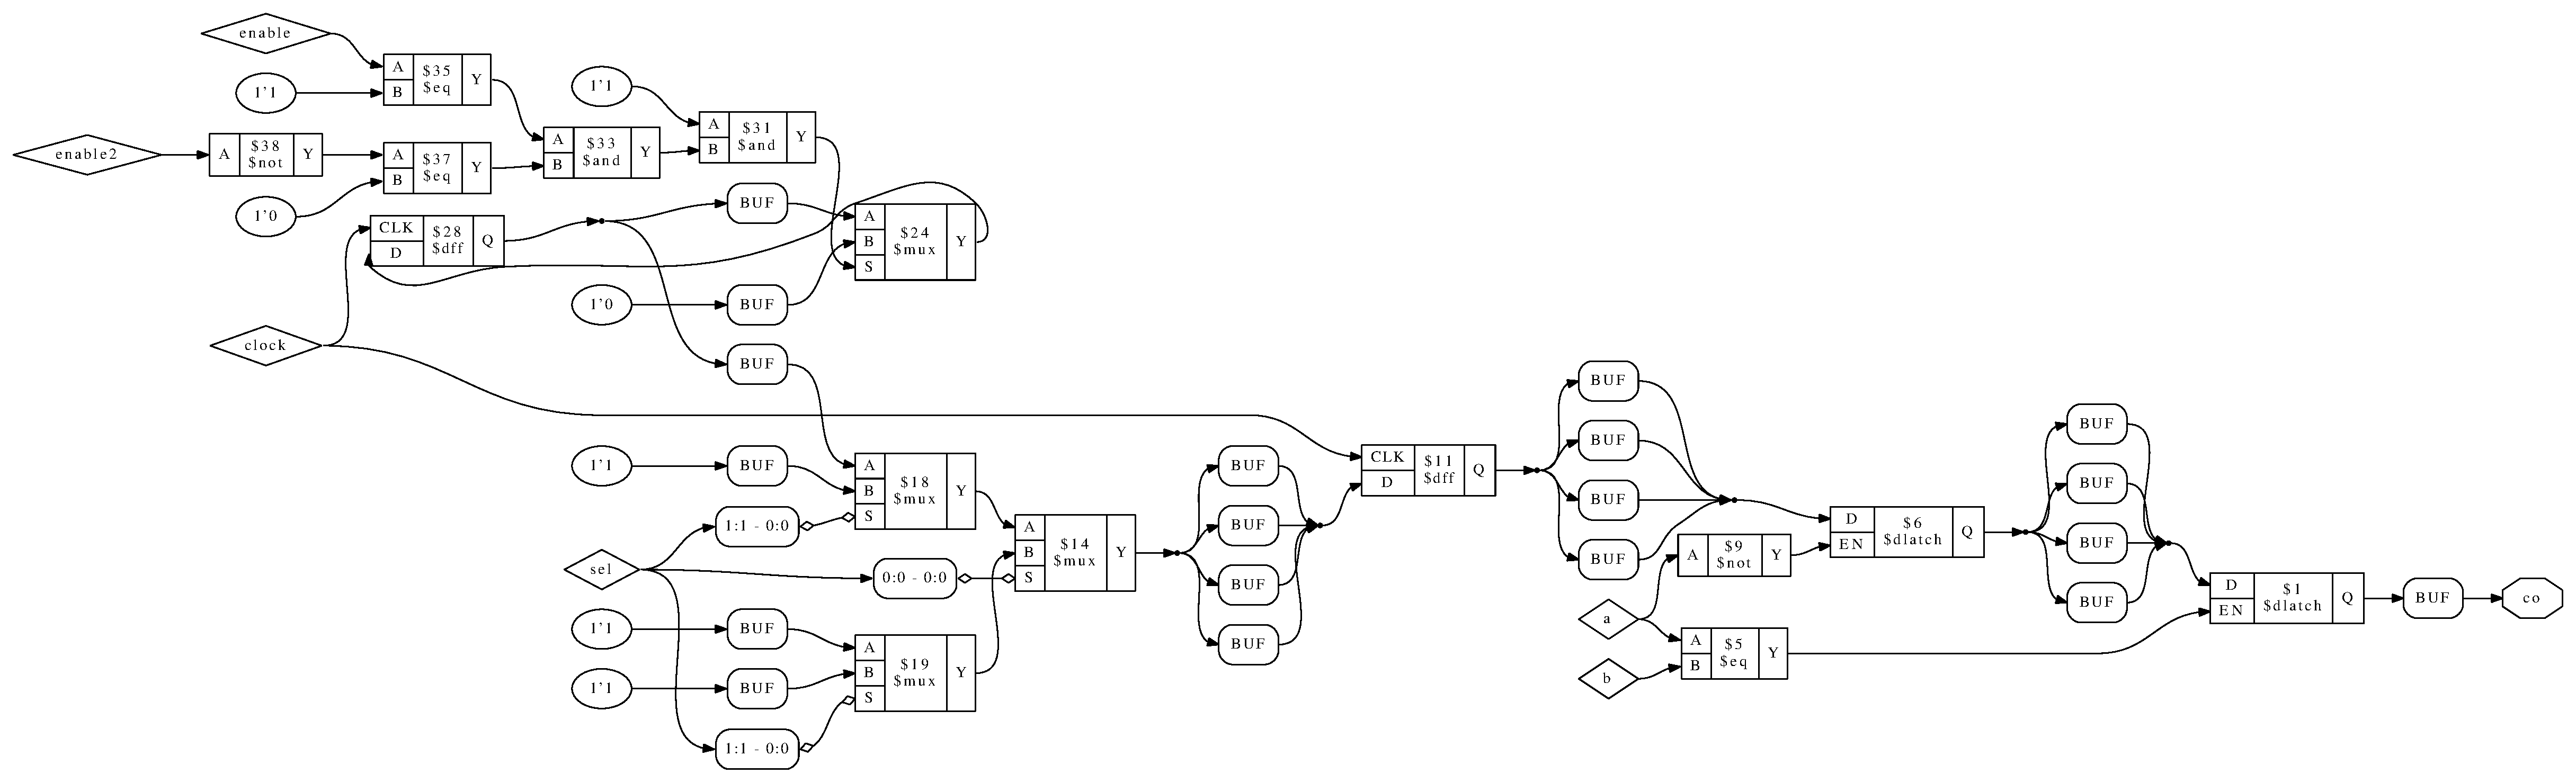
\includegraphics[width=1.2\textwidth]{synthesisShowcase/clusterfuck.eps}




\Large
    \textsf{by}

\vspace{0.5cm}

%\vspace*{\fill}

\LARGE
    \textsf{Florian Mayer}
    \vspace{1cm}

\vspace{1cm}

\flushleft
 \Large
\vspace*{\fill}

%-----------
\begin{tabbing}
    \textsf{Date of submission:} \= \textsf{15.09.2016} \kill
    \textsf{Date of submission:} \> \textsf{15.09.2016} \\
    \textsf{First corrector:} \> \textsf{Prof.\ Dr.\ Ludwig Frank}\\
    \textsf{Second corrector:} \> \textsf{Prof.\ Dr.\ Theodor Tempelmeier}
\end{tabbing}
%-----------

\end{titlepage}

\cleardoubleemptypage

{
\large
\thispagestyle{empty}
\vspace*{\fill}

\noindent
\textsc{Declaration of authorship}

\medskip

\noindent
I hereby declare that the thesis submitted is my own unaided work. All direct or indirect sources used are acknowledged as references.

I am aware that the thesis in digital form can be examined for the use of unauthorized aid and in order to determine whether the thesis as a whole or parts incorporated in it may be deemed as plagiarism. For the comparison of my work with existing sources I agree that it shall be entered in a database where it shall also remain after examination, to enable comparison with future theses submitted. Further rights of reproduction and usage, however, are not granted here.

This paper was not previously presented to another examination board and has not been published.

\bigskip

\noindent
Rosenheim, 15.09.2016

\vspace*{2cm}

\noindent
Florian Mayer
}

%%% Local Variables:
%%% mode: latex
%%% TeX-master: "d"
%%% End:

\chapter*{Kurzfassung}
\thispagestyle{empty}

Diese Arbeit beschreibt die Entwicklung des ersten open-source
VHDL-Frontends mit dem Namen Yodl. Yodl selbst benutzt das quelloffene
Synthesetoolkit Yosys als Basis.

Zunächst wird kurz der aktuelle Status der Entwicklung digitaler
Schaltungen reflektiert. Außerdem wird Yosys kurz beschrieben.
Danach beschreibt die Arbeit erst generelle,
compiler-spezifische Probleme, die gelöst werden müssen. Sodann geht
sie detailliert auf die VHDL-bezogenen Probleme ein und zeigt die
entwickelten Algorithmen und Design\-entscheidungen auf. Schließlich
liefert diese Masterarbeit einen Ausblick in die Zukunft von Yodl,
wobei hier
sowohl die momentanen Limitierungen der Implementierung als auch
Verbesserungen des Testsystems betrachtet werden.

Diese Abschlussarbeit dokumentiert und erklärt den Quellcode von
Yodl. Dieser liegt der Arbeit bei und ist gleichzeitig das wichtigste
Ergebnis.

Interessant ist sowohl der schriftliche als auch der Quellcodeteil
dieser Ausarbeitung für Hardwareentwickler, VHDL-Programmierer,
Yosys-Nutzer und Theoretiker aus dem Compilerbau und dem Gebiet der
formalen Sprachen. Insbesondere für Theoretiker ist der praktische
Aspekt dieser Arbeit relevant.

\bigskip

\noindent
Schlüsselworte: Compiler, Formale Sprachen, VHDL, Yosys, Hardwaresynthese
\chapter*{Abstract}
\thispagestyle{empty}
This work describes the development of the first open-source VHDL
frontend named Yodl. Yodl uses the synthesis toolkit Yosys as the
foundation.

First of all, the state-of-the-art of digital hardware design is
described. Furthermore, some details of the Yosys toolkit are
shown. After that, this work illustrates general, compiler-specific
problems any translation system faces during implementation. Then, the
thesis elaborates on the problems relevant to the processing of VHDL
code and shows the appropriate algorithms and design decisions the
project uses. Finally, this work provides a glance into the possible
future of Yodl where, among other things, current limitations and
improvements of the test system play an important role.

This thesis documents and explains the source code of Yodl which was
developed in the scope of this master thesis and also represents the
greatest achievement of it.

Both, the written part and the source code, might be of interest for
hardware developers, VHDL programmers, Yosys users, and theorists with
a background on compiler construction or formal languages. For
theoreticians, especially the practical aspects of this thesis are
likely to be relevant.

\bigskip

\noindent
Key words: Compiler, formal languages, VHDL, Yosys, hardware synthesis

\cleardoubleemptypage

\pagestyle{scrplain}
\pagenumbering{roman}
% ---------------------------------------------------
% D-TOC.TEX zur Verwendung mit TEXPART
% (an eigene Gegebenheiten anzupassen)
% ---------------------------------------------------
%
\tableofcontents
\clearpage
\listoffigures
\clearpage
\listoftables
\clearpage
\lstlistoflistings
\clearpage
\listofalgorithms
\cleardoublepage


\pagestyle{scrheadings}


\addtokomafont{caption}{\small}

\mainmatter

% TODO:
% Priozahl: Je höher desto unwichtiger!
% ----
% 2.2 Dann Grammarly
% TODO: add DFF to glossary
% TODO: Add STL to glossary
%%

\chapter{State-of-the-art of Hardwaredesign}
\label{ch:StateOfTheArt}

Today, almost every part of the work in digital hardware design is done
using sophisticated tools and integrated development
environments. This chapter will briefly elaborate on how digital
hardware is developed nowadays.

\section{VHDL}
\label{sec:VHDL}


The VHSIC Hardware Description Language (VHDL) is a language
originally intended for hardware simulation. Its history will not be
elaborated here because there already is comprehensive literature
about this topic \cite{VHDLHIST}.

VHDL quickly evolved from being just a hardware simulation tool
to a language that can also be compiled. Since VHDL describes
hardware, the target ``language'' is no language in the sense of x64 or
Motorola assembly, but rather a netlist (cyclic graph) of
cells connected through wires. Cells can be adders,
multipliers or subtraction units and are represented as vertices in
the netlist. Wires represent the interconnections between the
functional units in the netlist. The term signal vector or signal
chunk describes signals with \(n\)-bit width. A netlist can be coarsely
or finely grained, where a finely grained netlist is obliged to only
contain 1-bit input logic gates and 1-bit wide connections. This
limitation is not imposed on coarsely grained netlists. Those are even
allowed to contain abstractions for \(n\)-bit Multiplexers, etc.\
(cf. \cite{YOSYSRM} chapter 4.2).

To give an intuition of what hardware design with VHDL looks
like, listing \ref{fulladd} presents a hardware model of a 1-bit wide
full adder.

The identifiers \VH{a}, \VH{b}, \VH{carryIn}, \VH{carryOut} and
\VH{sum} are signals
of the top level entity of this model. All those \emph{top-level}
signals can have a type, in this case \VH{std_logic}, and a direction,
either \VH{in}, \VH{out} or \VH{inout}. The type \VH{std_logic}
declares all signals to be of 1-bit width.
\VH{Entity} declarations describe the interface of a hardware
module, whereas \VH{architecture} blocks define the netlist of the
previously declared entity.

In \VH{architecture} \VH{behv}, two statements are present. These are
called \emph{signal assignment statements}. The arrow is used to
connect two signals together and operators like \VH{xor} or \VH{and}
define hardware functionality. Adders would thus be described by the
operator \VH{+}.

\begin{lstlisting}[style=vhdl,caption={Simple full adder in
      vhdl},label=fulladd, float=tb]
entity adder is
   port(a        : in  std_logic;
        b        : in  std_logic;
        carryIn  : in  std_logic;
        carryOut : out std_logic;
        sum      : out std_logic);
end adder;

architecture behv of adder is
begin
   sum <= a xor b xor carryIn;
   carryOut <=    (a and b)
               or (b and carryIn)
               or (a and carryIn);
end behv;
\end{lstlisting}
%
Since the code in \ref{fulladd} is synthesizeable, a netlist can be
compiled from the source. For the model given above, the result is
shown in figure \ref{fig:netlistAdder}.
Note how the semantics of listing \ref{fulladd} and graph
\ref{fig:netlistAdder}
have not changed; illustration \ref{fig:netlistAdder} describes exactly
the same data flow as figure \ref{fulladd}. Only the representation of
the hardware description has changed.

In real life, however, hardware designs are much more complicated than
in listing \ref{fulladd}. Because of the incredible complex designs
arising in
modern hardware industry, VHDL became a viable tool, as it is obvious
that the construction of netlists by hand like figure
\ref{fig:netlistAdder},
does not scale well especially if more than one person is involved in a
design project.
%
\begin{figure}[tb]
\caption{Netlist example for a binary adder}
\centering
    \begin{dot2tex}[graphstyle={shorten >=1pt,shorten <=1pt},
    options={--autosize}]

    digraph G {
      node [shape="box"];
      a -> xor1;
      b -> xor1;
      xor1 -> xor2;
      carryIn -> xor2;
      xor2 -> sum;

      a -> and1;
      b -> and1;

      a -> and2;
      carryIn -> and2;

      b -> and3;
      carryIn -> and3;

      and1 -> or1;
      and2 -> or1;

      or1 -> or2;
      and3 -> or2;

      or2 -> carryOut;

      and1 [shape="circle", label="and"];
      and2 [shape="circle", label="and"];
      and3 [shape="circle", label="and"];

      or1 [shape="circle", label="or"];
      or2 [shape="circle", label="or"];

      xor1 [shape="circle", label="xor"];
      xor1 [shape="circle", label="xor"];
    }
    \end{dot2tex}
\label{fig:netlistAdder}
\end{figure}
\section{Yosys}
\label{sec:Yosys}

Yodl -- the tool described in this work -- is based on Yosys. Yosys is
an open-source logic
synthesis toolkit with various other features. It is actively
maintained by Clifford Wolf, who also did almost all of the
implementation work (cf. \cite{YOSYSRM}).

Like in so many other topics in science and engineering, different layers
of abstraction help to make hardware design automation
feasible. Figure \ref{fig:abstractions} shows such a layer
stack (cf. \cite{YOSYSRM} chapter 2.1). Note that
\ref{fig:abstractions} is not a comprehensive depiction of those layers.
%
\begin{figure}[t]
\caption{Abstraction hierarchy}
    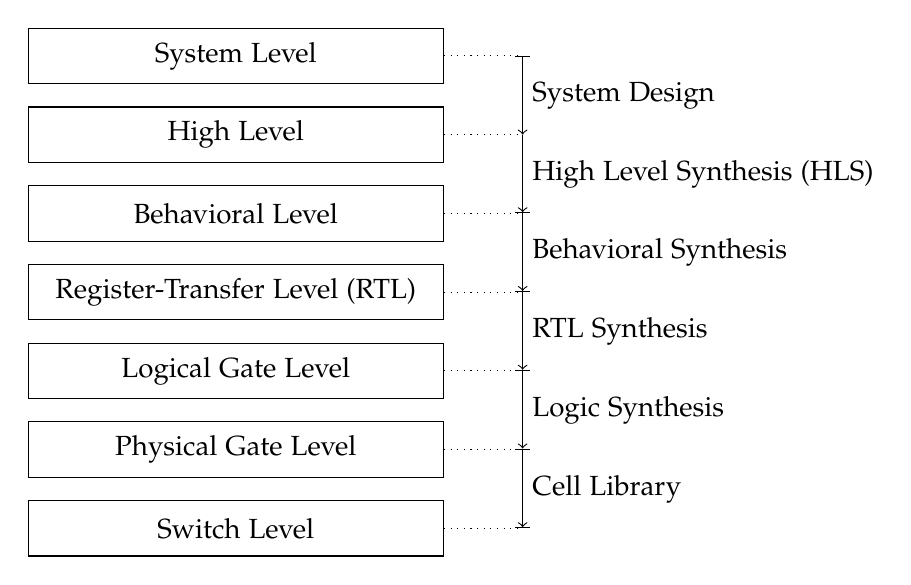
\begin{tikzpicture}
        \tikzstyle{lvl} = [draw, rectangle, minimum height=2em, minimum width=15em]
        \node[lvl] (sys) {System Level};
        \node[lvl] (hl) [below of=sys] {High Level};
        \node[lvl] (beh) [below of=hl] {Behavioral Level};
        \node[lvl] (rtl) [below of=beh] {Register-Transfer Level (RTL)};
        \node[lvl] (lg) [below of=rtl] {Logical Gate Level};
        \node[lvl] (pg) [below of=lg] {Physical Gate Level};
        \node[lvl] (sw) [below of=pg] {Switch Level};
        \draw[dotted] (sys.east)  -- ++(1,0) coordinate (sysx);
        \draw[dotted] (hl.east)  -- ++(1,0) coordinate (hlx);
        \draw[dotted] (beh.east) -- ++(1,0) coordinate (behx);
        \draw[dotted] (rtl.east) -- ++(1,0) coordinate (rtlx);
        \draw[dotted] (lg.east)  -- ++(1,0) coordinate (lgx);
        \draw[dotted] (pg.east)  -- ++(1,0) coordinate (pgx);
        \draw[dotted] (sw.east)  -- ++(1,0) coordinate (swx);

        \draw[|->] (sysx) -- node[right] {System Design} (hlx);
        \draw[->|] (hlx) -- node[right] {High Level Synthesis (HLS)} (behx);
        \draw[->|] (behx) -- node[right] {Behavioral Synthesis} (rtlx);
        \draw[->|] (rtlx) -- node[right] {RTL Synthesis} (lgx);
        \draw[->|] (lgx) -- node[right] {Logic Synthesis} (pgx);
        \draw[->|] (pgx) -- node[right] {Cell Library} (swx);
    \end{tikzpicture}
    \label{fig:abstractions}
\end{figure}
%
Yosys acts on the abstraction levels \emph{Behavioral Level},
\emph{RTL Synthesis} and \emph{Logic Synthesis}, but it does not
implement every algorithm for the transitions between these layers
itself. While \emph{Logic Synthesis} can be done entirely using
the own
logic synthesis algorithms of Yosys, the toolkit also provides an interface to
a logic synthesis toolchain called \emph{ABC} which is recommended to
be used (cf. \cite{YOSYSRM} chapter 2.1.5 page 16).
An in-depth introduction to either one of the depicted levels is
beyond the scope of this work. However, chapter 1 of \cite{MSEM}
provides an introduction to the topic.

A high-level overview of the architecture of Yosys is necessary,
especially for later chapters where Yosys is directly
interfaced. Figure \ref{fig:yosysArch} gives such a birds-eye view and
shows how the different components of the toolchain work
together. RTLIL and AST are data structures located in memory during the
execution of Yosys. RTLIL represents netlists, whereas AST depicts generic
abstract syntax trees. Yosys makes it possible to add the VHDL frontend
component at two places. First, the frontend could produce an abstract
syntax tree using the predefined AST format from Yosys, thus the
component would be placed above AST. Second, the
VHDL component could emit an RTLIL netlist serialized to normal ASCII
text. Said text would then be put into the ilang frontend that does
the deserialization. The AST frontend of Yosys is used to convert the
AST format into RTLIL netlists. Note that there are various ways to
output RTLIL structures. The Verilog backend, for example, generates
plain register transfer level Verilog code, whereas the Graphviz
backend serves as tool for netlist visualization. Finally, Yosys
provides optimizations that act only on RTLIL netlists. Chapter
\ref{sec:rtlilStruct} illustrates the format of those netlists. There
are, for instance, optimization passes that eliminate process objects
or similar high-level constructs from the netlists and replace them by
simple logic cells or wires.

\begin{figure}[tb]
\caption{Main Yosys components and data structures}
\centering
    \begin{dot2tex}[dot, tikz, options={--autosize}]

        digraph A {
          graph [splines=true, overlap=prism];
          nVerF [shape=box, label="Verilog frontend"];
          nVhdF2 [shape=box, label="VHDL frontend", style=dotted];
          nVhdF [shape=box, label="Yodl", color=red];
          nIlangF [shape=box, label="Ilang frontend"];
          nOtherF [shape=box, label="Other frontends"];

          nVerB [shape=box, label="Verilog backend"];
          nIlangB [shape=box, label="Ilang backend"];
          nOtherB [shape=box, label="Other backends"];
          nDotB [shape=box, label="Graphviz backend"];

          passes [shape=ellipse, label="Transformations"];

          nAstF [shape=box, label="AST frontend"];
          ast [label="AST", color=orange];
          rtlil [label="RTLIL", color=orange];


          nVerF:s -> ast:n;
          nVhdF2:s -> ast:n;
          nVhdF:s -> nIlangF:n;
          nIlangF:s -> rtlil:n;
          nOtherF:s -> rtlil;
          ast:s -> nAstF:n;

          {
            rank=same
            rtlil -> passes;
            passes -> rtlil;
          }

          nAstF:s -> rtlil:n;
          rtlil:s -> nIlangB:n;
          rtlil:s -> nVerB:n;
          rtlil:s -> nOtherB:n;
          rtlil:s -> nDotB;
        }
    \end{dot2tex}
    \label{fig:yosysArch}
\end{figure}

\section{Yodl}
\label{sec:Yodl}

Yodl is a standalone program that generates Ilang code. Ilang code, is
just another representation of RTLIL from figure \ref{fig:yosysArch}
and as such it is just a netlist. Yodl, in turn, uses VHDL files as
input in order to generate those netlists. So, consequently, Yodl
transforms VHDL code into RTLIL. The details regarding this
transformation will be explained in detail in chapter
\ref{ch:YodlImplDetails}. The same chapter also contains information
about the RTLIL.

Yodl is not a production ready synthesis system yet. The current
limitations are listed in chapter \ref{sec:currentLimits}. During the
development of Yodl, a subset of VHDL has been developed to hide some
complexities not regarded in this work. The subset is called SVHDL (S
for simple) and is specified briefly and informally in chapter
\ref{sec:svhdl}.

As stated in the abstract, a major achievement of this thesis is the
implementation of Yodl itself. The entire source code is available
on Github: \url{https://github.com/forflo/yodl}. File names referring
to sources in this repository are printed \texttt{using this font} and,
unless otherwise noted, are relative to
\url{https://github.com/forflo/yodl/tree/master/vhdlpp}.

\chapter{Yodl -- Subproblems}
\label{ch:YodlSubproblems}

Any compiler construction project can be split up into three distinct
subprojects: Lexis and Syntax, validity checks regarding the semantics
and code/hardware generation. The last step, hardware generation, is
also usually referred to as \emph{synthesis}. The first section of this
chapter shows the parsing and lexing problems caused by VHDL's
unorthodox grammar. Section two briefly describes the concept of
language
semantics and answers the question why Yodl can't provide proper
compile-time semantics checks. The last part of the problem,
synthesis, will not be elaborated here because chapter
\ref{ch:YodlImplDetails} contains detailed information about this topic.

\section{Lexis and Syntax}
\label{sec:LexisAndSyntax}

%TODO: AST into glossary
%      Sources for the term concrete syntax

In order to process a programming language of any kind, an abstract syntax
tree (AST) has to be constructed. A software component
called \emph{parser} usually does that. The parser takes tokens
produced by a tokenizer
(also called lexer) and incrementally builds said AST. In theory,
every programming language can be expressed using only one formal
grammar (concrete syntax).
However, this grammar would even have to include rules
describing how identifiers, numbers or even strings can be
constructed, making it very convoluted -- and as a consequence -- harder to
understand. Thus, a two-layer approach is used ever since the very
first compilers were built. The first layer solely contains the lexical
analysis. In it, every token (parentheses, identifiers, operator
symbols \ldots) is described by a corresponding regular
expression. The result of the first step is a sequence of tokens
which the parser uses for the second step.
This second step consists of a parsing algorithm that can match
context-free grammars (mostly of type LALR(1)). The vast set of %TODO footnote?
details bound to formal languages and, in consequence, parsing in
general, is beyond the scope of this document and will not be elaborated.

Since the rise of parser generators (such as YACC in the early 1970s)
very efficient parsers can be automatically generated from context
free grammars
encoded in BNF (Backus-Nauer Form). The majority of these code generators
put certain restrictions onto the grammars which they can
process. Grammars usually have to be in a well-defined subset of the
set of the context-free languages; LALR(1) is such a subset. In order
for a language to be an element of LALR(1), it must not contain any
shift/reduce or reduce/reduce conflicts. This property can be
mechanically checked using sophisticated mathematical algorithms
(cf. \cite{LRKNUTH}).

VHDL is a special case because its grammar neither is a member of LR(1)
-- a superclass of LALR(1) -- nor LALR(1). To proof this, a part of
VHDL's grammar is examined.


\begin{grammar}
<name> ::=
  <simple_name> \alt <operator_symbol>
\alt <character_literal> \alt <selected_name>
\alt <indexed_name> \alt <slice_name>
\alt <attribute_name>

<function_call> ::=
<name> [ `(' <association_list> `)' ]

<association_list> ::=
<association_element> \{ , <association_element> \}

<association_element> ::=
[ <formal_part> `=>' ] <actual_part>

<formal_part> ::=
  <name>
\alt <name> `(' <name> `)'

<actual_part> ::=
  <actual_designator>
\alt <name> `(' <actual_designator> `)'

<expression> ::= <name> \alt <number>

<actual_designator> ::=
[ `inertial' ] <expression>
\alt <name>
\alt `open'

<prefix> ::= <name> \alt <function_call>

<selected_name> ::= <prefix> `.' <suffix>

<attribute_name> ::= <prefix> `'' <attribute_designator> [ `(' <expression> `)' ]

<slice_name> ::= <prefix> `(' <discrete_range> `)'

<indexed_name> ::= <prefix> `(' <expression> \{ `,' <expression> \} `)'

<operator_symbol> ::= <string_literal>

<character_literal> ::= `'' <graphic_character> `''
\end{grammar}
%
Although this is only a very small subset of the VHDL grammar, it is
still hard to see the ambiguity. The following paragraph will present
a set of valid simplification steps, that produce subsets of the
grammar listed above.
The removal of any grammar rules and
non-terminal symbols does not create ambiguities but
only a new subset of the original language.
The idea behind this proof is, to keep deleting non-terminals and
grammar rules until it becomes obvious enough to trivially show the
existence of
a reduce/reduce or shift/reduce conflict. Since only a
strict subset of the grammar remains, the proof is sound.

The deletion of the following non-terminals, serves as start.
\begin{grammar}
<operator_symbol> ::= <string_literal>

<character_literal> ::= `'' <graphic_character> `''
\end{grammar}
%
Since ``slice_name'' can be expressed by the non-terminal
``indexed_name'' the following can also be deleted:
%
\begin{grammar}
<slice_name> ::= <prefix> `(' <discrete_range> `)'
\end{grammar}
%
Also, the rules
\begin{grammar}
<selected_name> ::= <prefix> `.' <suffix>

<attribute_name> ::= <prefix> `'' <attribute_designator> [ `(' <expression> `)' ]
\end{grammar}
get deleted.

Furthermore, simplification can be done by defining function calls to
be productions of
\begin{grammar}
<function_call> ::=
<name> [ `(' { <expression> } `)' ]
\end{grammar}
%
This produces a language subset, where only unary functions can be
called.

After these subsetting steps, only the following grammar remains.
Note that \emph{prefix} does not exist because it has been subsumed by
\emph{indexed_name}.
\begin{grammar}
<name> ::=
  <simple_name>
\alt <indexed_name>

<function_call> ::=
<name> [ `(' { <expression> } `)' ]

<expression> ::= <name> \alt <number>

<indexed_name> ::= <name> `(' <expression> \{ `,' <expression> \} `)'
\alt <function_call> `(' <expression> \{ `,' <expression> \} `)'
\end{grammar}
%
The reduce/reduce conflict indeed is obvious now.
It shows up clearly if one creates
two different production sequences that generate the same
sequence of tokens.
%
\begin{grammar}
<name> ::= <indexed_name> ::= <name> `(' <expression> `)' ::= `foo'
`(' 42 `)'

<name> ::= <indexed_name> ::= <function_call> ::= <name> `('
<expression> `)' ::= `foo' `(' 42 `)'
\end{grammar}
%
Reduce/reduce errors generally imply a bad language design. But as mentioned
before, VHDL is a special case. It simply might not be possible to create a
conflict free context-free grammar where function parameter lists and
array subscriptions both use the same parameter/expression grouping
symbol; namely ``('' and ``)''.

Fortunately, there is a way to resolve this ambiguity. Given the
following VHDL snippet \ref{vhdlAmbigSnippet}
%
\begin{lstlisting}[style=vhdl, caption={Example of a syntactically
      ambiguous VHDL snippet}, label=vhdlAmbigSnippet]
entity ent is
   port(A     : out  std_logic_vector(1 downto 0));
end ent;

architecture beh of ent is
   signal foo : std_logic_vector(1 downto 0);
begin
   A(1) <= foo(0);
   A(0) <= foo(1);
end beh;
\end{lstlisting}
%
The ambiguity can be resolved with the help of the context. In
particular the scoping information can be used to figure out whether a
name refers to a variable, a type, or a function.
In the above source code, this is easy. Since \VH{A} is declared to
be an output signal and \VH{foo} is a signal local (i.e. only
visible) inside the enclosing architecture and
because both signals are of type \VH{std_logic_vector}, it can be
inferred that \VH{A(1)} clearly describes an array subscription.

In order to generate an
unambiguous AST, this information needs to be processed by the
parser. To be specific, the parser needs to keep track of a scope
stack and all visible identifiers, which makes it a scope aware
parser. Because the implementation of such a context sensitive parser
would probably be enough to provide material for an entire
thesis, an existing VHDL parser will be reused for the purpose
presented in this master thesis (cf. \ref{ch:YodlImplDetails}).

\section{Compile-time checks}
\label{sec:Compile-time checks}

Compile-time checks are also commonly referred to as semantic
checks. In formal language theory, there generally are two kinds of
semantics that can be defined: The \emph{static} semantics and
\emph{dynamic} semantics. Both formalisms use the previously defined
abstract syntax to give a formal specification and assume only
syntactically correct programs as input.
Simply put, static semantics describe properties of a program that can
be verified during compile time. Hence the term \emph{static}. The
type system of a programming language belongs to this semantic
class. In the context of VHDL, for example, the correct usage of
packages or libraries must be verifiable during translation time too,
thus checks regarding those issues are part of a static semantic
specification (cf. introductory chapters of \cite{FERN2014} and
\cite{SCH97}).

The dynamic semantics of a program is either a rigid description of
its behavior during runtime (i.e. how does the program manipulate
data) or a specification of the end-product to the translation process
(i.e. a netlist).

Unfortunately, IEEE 1076-2008, \cite{IEEELRM},
does not give a formal set of rules using mature mathematical
frameworks for semantic specifications. Rather, it provides
a language description in English (which is a natural language and not
meant to be used as a rigid formal tool).

In 1995, however, the formal specification \cite{VHDLFORM}
was published which defines VHDL with different mathematical
tools. Since then, sadly there hasn't been made any update for this
work whatsoever, making it obsolete as the current standard outdates
this work by 13 years.

As a consequence, this work will not present any compile-time
consistency/semantic checks.

\chapter{Yodl -- Implementation details}
\label{ch:YodlImplDetails}

This chapter will elaborate on information around the actual
implementation of the VHDL frontend Yodl. The first chapter examines
the infrastructure that has been built. The following chapter
describes the various AST transformation passes. The
last chapter finally gives information about the netlist generator
algorithm and Yodl's current limitations.
%
\begin{lstlisting}

\end{lstlisting}
%
Before the first section of this chapter begins, the overall mode of
operation of Yodl must be clarified. As chapter \ref{sec:Yodl} briefly
states, Yodl transforms plain VHDL code into RTLIL netlists. In order
to accomplish this, Yodl first reads in the VHDL source and constructs
a tree structure representing the code. The scanner component
tokenizes the input code according to the language standard and passes
the tokens to the parser, which gradually constructs the parse tree
(AST) from the bottom up. Unnecessary information gets discarded during
scanning and parsing. For example, parentheses or other structuring
tokens need not be contained in the tree representation, because the
structure of the tree already provides the same information in a much
more usable manner. Chapter \ref{sec:LexisAndSyntax} regards some of
the more difficult problems in the scanning and parsing parts.

Once Yodl possesses an AST, it must be
semantically checked; though this step is currently
omitted. Thereafter, AST simplification happens. Compile-time
evaluable expressions get evaluated and replace their originals, loops
get unrolled, generate statement evaluation happens and syntax sugar
gets replaced by simpler, semantically equivalent language
primitives. The order of these simplification steps is not hard-wired
and can easily be adjusted. Also, they are elaborated in chapter
\ref{sec:astTrans}.

Finally, Yodl conducts the netlist
synthesis and emits the serialized netlist to an IO stream. Yodl
currently does not do anything besides AST simplification and netlist
generation because of the limitations listed at the end of this
chapter. Note that figure \ref{fig:yosysArch} puts Yodl in the greater
context of the Yosys toolchain and shows how frontend and backend are
intertwined. Furthermore, section \ref{sec:RTLILgeneration} documents
the creation of netlists.

\section{Infrastructure}
\label{sec:Infrastructure}

\subsection{Data model}
\label{sec:DataModel}

As \ref{sec:LexisAndSyntax} mentioned, Yodl reuses an existing parser
for VHDL. This parser comes from the project \emph{vhdlpp} \cite{VHDLPP}.
Vhdlpp already includes a lexer, a parser and suitable classes that
describe the abstract syntax tree.

The data model uses inheritance in order to resemble the nature of the
productions in the grammar. The principle used, can be explained best
using a simple expression grammar.
%
\begin{grammar}
<Exp>  ::= <Exp>  "+" <Exp1> \alt <Exp1>;

<Exp1> ::= <Exp1> "*" <Exp2> \alt <Exp2>;

<Exp2> ::= <Integer> \alt "(" <Exp> ")";
\end{grammar}
%
A set of data types can now be defined that might be used to build a
typed AST for this grammar. Listing \ref{lst:expGrammar} shows one
possible implementation. Using the data types from listing
\ref{lst:expGrammar}, the representation of the expression \(1+3*4+3\)
is as simple as code \ref{lst:expGrammarRep}.
%
\begin{lstlisting}[style=c++, caption={Class hierarchy for a simple
      expression grammar}, label={lst:expGrammar}]
class Exp { virtual ~Exp() = default; };

class EAdd : public Exp {
public:
  Exp *exp_1; Exp *exp_2;
  EAdd(Exp *p1, Exp *p2);
};

class EMul : public Exp {
public:
  Exp *exp_1; Exp *exp_2;
  EMul(Exp *p1, Exp *p2);
};

class EInt : public Exp {
public:
  Integer integer_;
  EInt(Integer p1);
};
\end{lstlisting}
%
\begin{lstlisting}[style=c++, caption={Representation of \((1+3)*(4+3)\)},
    label={lst:expGrammarRep}]
Exp *expression = new EMul(
    new EAdd(new EInt(1), new EInt(3)),
    new EAdd(new EInt(4), new EInt(3)));
\end{lstlisting}
%
Listing \ref{lst:expGrammar} contains one base class \CPP{Exp} and
three derived classes that inherit from it. Since the destructor
function of the base is marked \CPP{virtual} and \CPP{default}, the
inheritance tree is polymorphic and, consequently, the compiler
generates a V-Table for each child of \CPP{Exp}. Those V-Tables serve
two purposes. First of all, they enable virtual dispatch and Secondly,
V-Tables are needed for runtime type analysis of polymorphic objects.
After all, the cast operator of C++, \CPP{dynamic_cast}, can only do
downcasts on polymorphic objects. Type analysis enables
one to determine whether a pointer of type \CPP{Exp} points to
\CPP{EAdd} or any other specialization of that same base class. In
other words, a polymorphic inheritance relation that models a formal
grammar,
can be used to create typed abstract syntax trees, where the type
information of the respective nodes is implicitly available through the
V-Tables attached to every object and can be explicitly queried using
\CPP{dynamic_cast}. The details of queries of this nature are a
idiosyncracy of C++ and shall not be elaborated any further here.

The main purpose of the method illustrated in listing
\ref{lst:expGrammar} is therefore the creation of typed ASTs.

Listing \ref{lst:expGrammarRep} shows the creation of a typed
abstract syntax tree. Once created, the tree begins with an
\CPP{EMul} object as
root containing two pointers. Both point to a distinct \CPP{EAdd}
object which, in turn, also point to two \CPP{EInt} objects
respectively. \CPP{EInt(3)}, for example, can be reached using the
path \CPP{EMul::exp_1} \(\to\) \CPP{EAdd::exp_2}.

For reference, figure \ref{fig:classHier} shows the inheritance
relation between all
relevant classes of the data model of the AST that Yodl uses
internally for VHDL code. This model is
constructed using the same
principles, that the listings
\ref{lst:expGrammar} and \ref{lst:expGrammarRep} demonstrate.
That means, each actual node can be of a non-virtual class
type that is present in the illustrated inheritance tree.

\begin{figure}[p]
    \centering
    \caption{Class hierarchy of the AST's data model}
    \resizebox{\textwidth}{!}{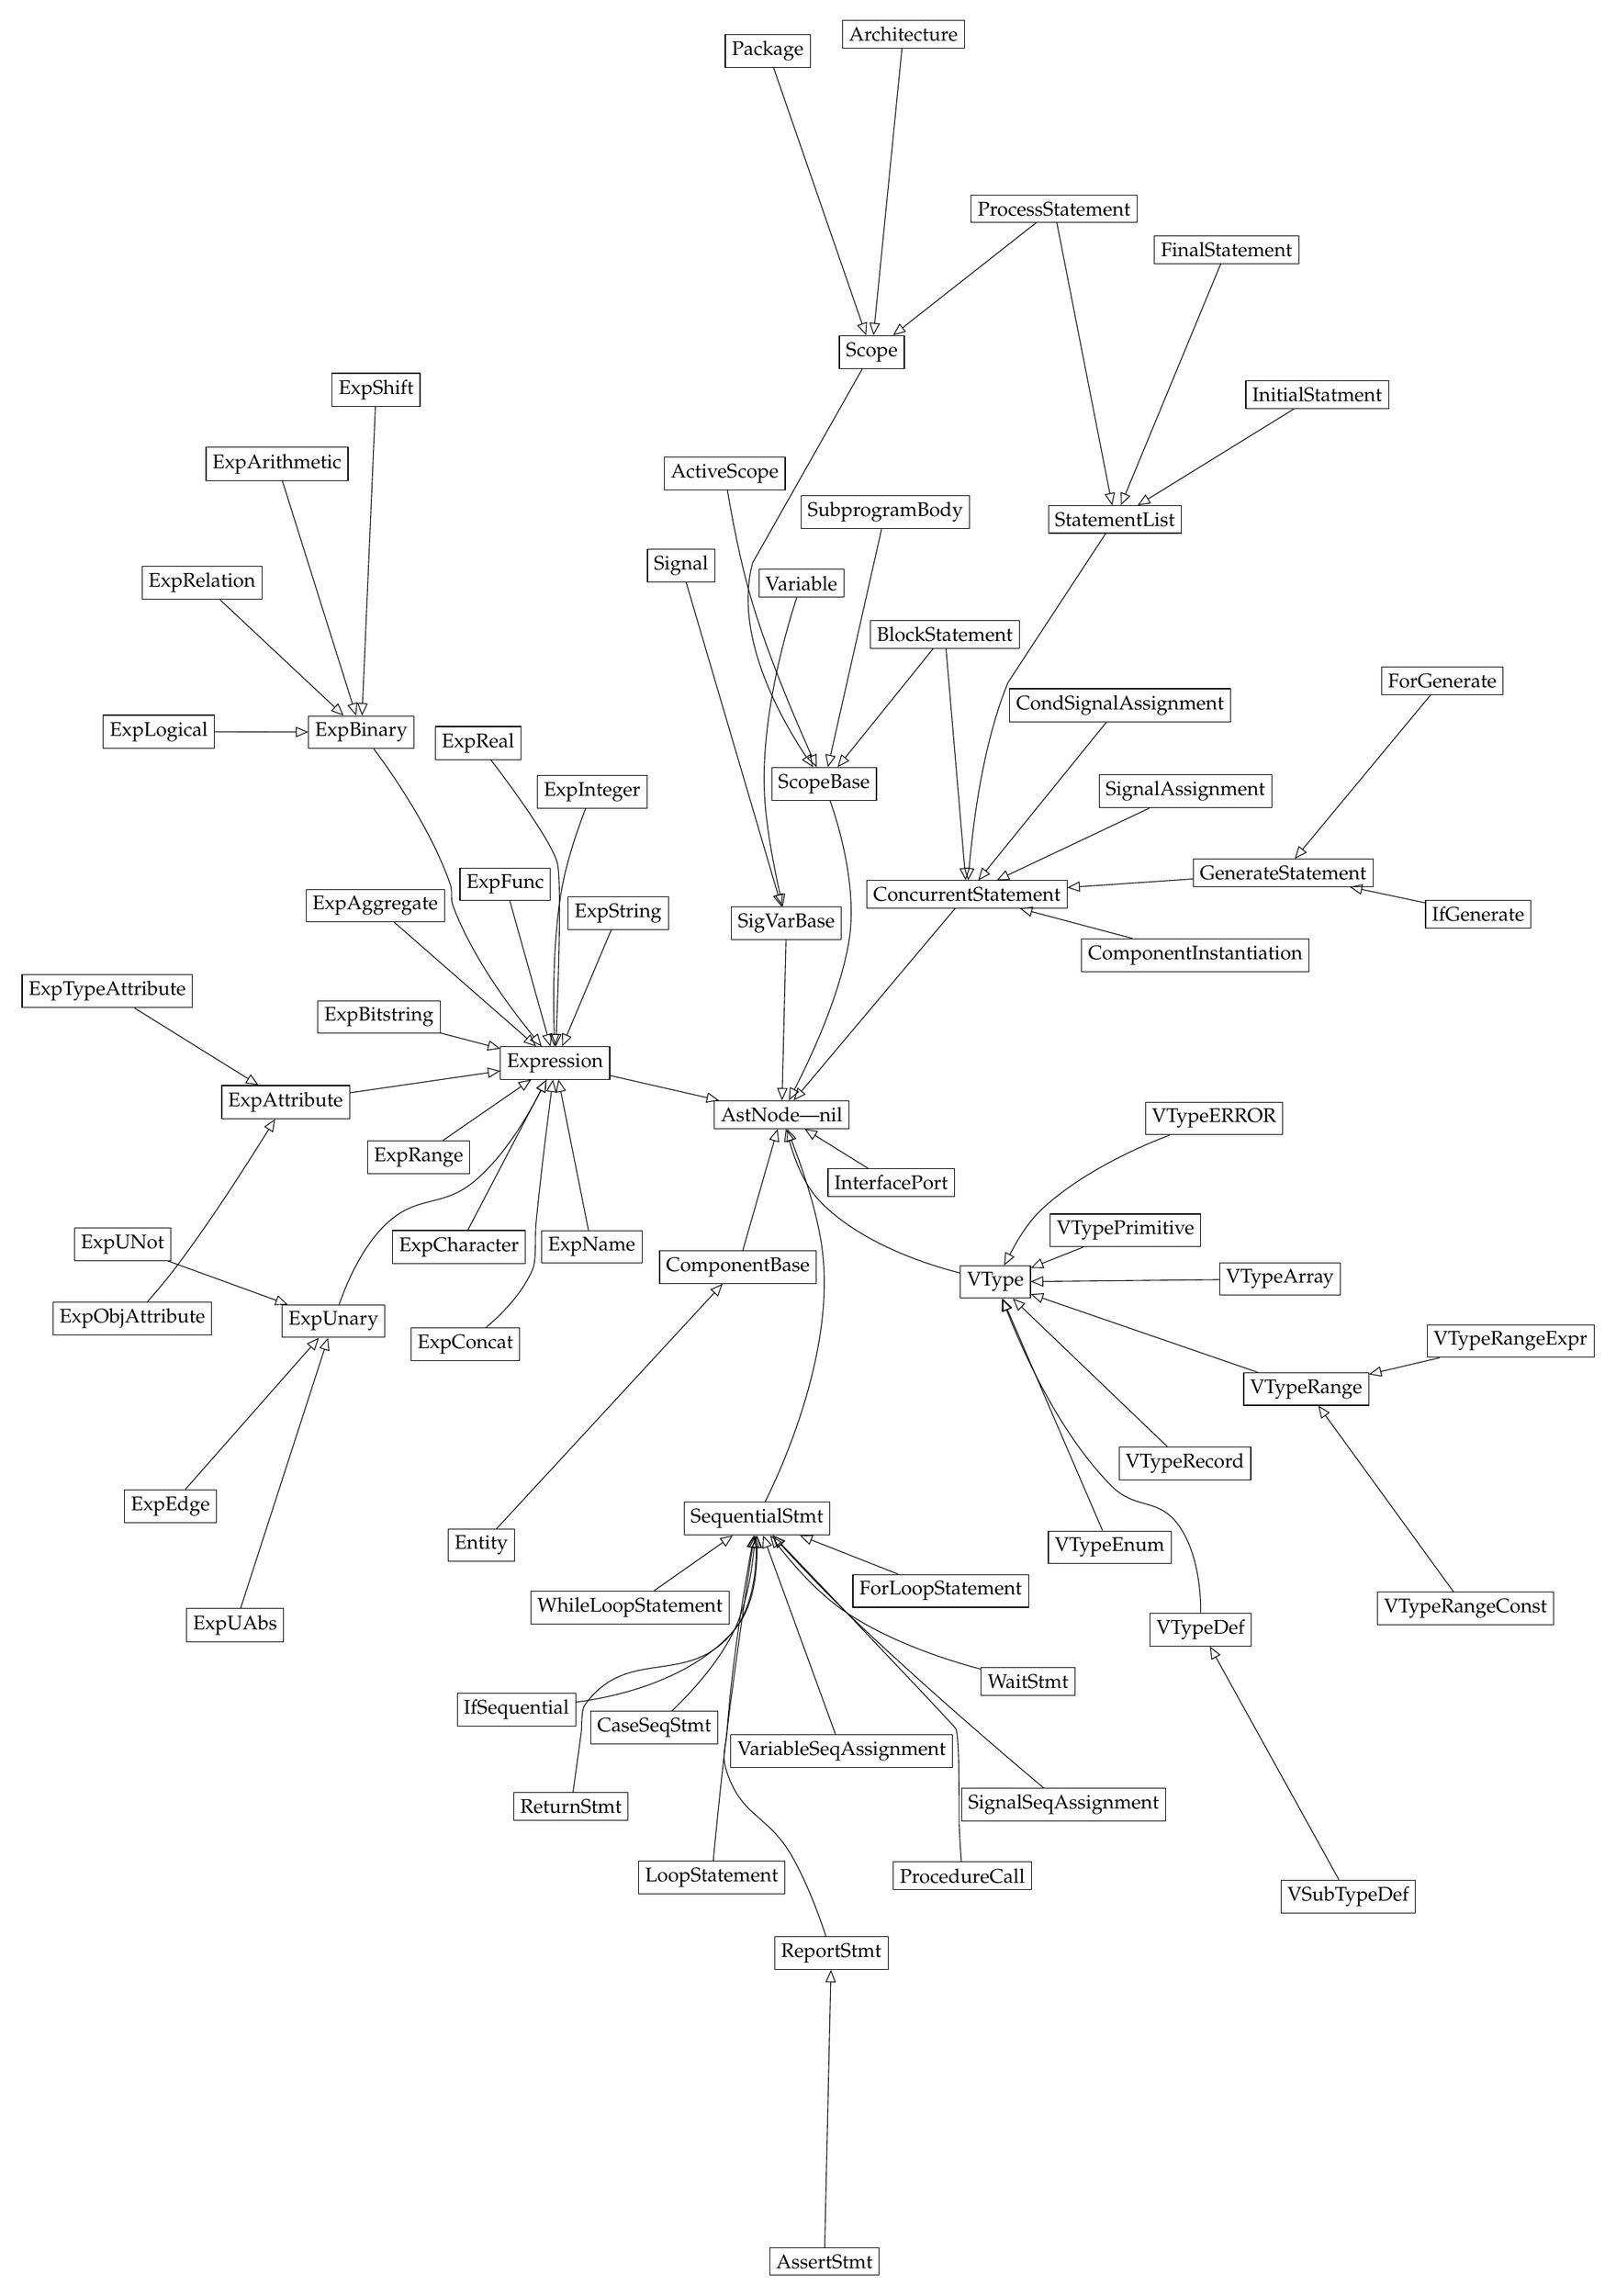
\begin{tikzpicture}%
\begin{scope}
  \pgfsetstrokecolor{black}
  \definecolor{strokecol}{rgb}{1.0,1.0,1.0};
  \pgfsetstrokecolor{strokecol}
  \definecolor{fillcol}{rgb}{1.0,1.0,1.0};
  \pgfsetfillcolor{fillcol}
  \filldraw (0.0bp,3.91bp) -- (0.0bp,1141.39bp) -- (795.34bp,1141.39bp) -- (795.34bp,3.91bp) -- cycle;
\end{scope}
  \node (ForLoopStatement) at (464.7bp,349.13bp) [draw,rectangle] {ForLoopStatement};
  \node (VTypePrimitive) at (558.04bp,531.01bp) [draw,rectangle] {VTypePrimitive};
  \node (GenerateStatement) at (637.58bp,711.35bp) [draw,rectangle] {GenerateStatement};
  \node (SignalSeqAssignment) at (526.75bp,241.3bp) [draw,rectangle] {SignalSeqAssignment};
  \node (ExpUNot) at (51.689bp,523.9bp) [draw,rectangle] {ExpUNot};
  \node (ExpBitstring) at (181.15bp,638.64bp) [draw,rectangle] {ExpBitstring};
  \node (ExpName) at (288.56bp,522.64bp) [draw,rectangle] {ExpName};
  \node (Statement) at (477.94bp,700.44bp) [draw,rectangle] {ConcurrentStatement};
  \node (VariableSeqAssignment) at (414.67bp,268.34bp) [draw,rectangle] {VariableSeqAssignment};
  \node (VTypeEnum) at (550.03bp,371.14bp) [draw,rectangle] {VTypeEnum};
  \node (Scope) at (429.94bp,974.03bp) [draw,rectangle] {Scope};
  \node (ProcessStatement) at (521.94bp,1046.3bp) [draw,rectangle] {ProcessStatement};
  \node (ExpAttribute) at (134.03bp,595.66bp) [draw,rectangle] {ExpAttribute};
  \node (ScopeBase) at (405.86bp,756.18bp) [draw,rectangle] {ScopeBase};
  \node (AstNode) at (384.43bp,589.32bp) [draw,rectangle] {AstNode|nil};
  \node (Signal) at (333.7bp,866.35bp) [draw,rectangle] {Signal};
  \node (VTypeRangeConst) at (729.64bp,340.33bp) [draw,rectangle] {VTypeRangeConst};
  \node (VTypeArray) at (636.02bp,506.43bp) [draw,rectangle] {VTypeArray};
  \node (ExpUAbs) at (108.55bp,331.86bp) [draw,rectangle] {ExpUAbs};
  \node (ExpArithmetic) at (129.7bp,917.55bp) [draw,rectangle] {ExpArithmetic};
  \node (WaitStmt) at (508.81bp,303.39bp) [draw,rectangle] {WaitStmt};
  \node (SignalAssignment) at (588.24bp,752.56bp) [draw,rectangle] {SignalAssignment};
  \node (ExpUnary) at (158.19bp,485.17bp) [draw,rectangle] {ExpUnary};
  \node (AssertStmt) at (405.98bp,10.906bp) [draw,rectangle] {AssertStmt};
  \node (FinalStatement) at (609.01bp,1025.6bp) [draw,rectangle] {FinalStatement};
  \node (ExpFunc) at (244.86bp,705.53bp) [draw,rectangle] {ExpFunc};
  \node (ExpRange) at (201.2bp,567.88bp) [draw,rectangle] {ExpRange};
  \node (IfGenerate) at (736.07bp,690.52bp) [draw,rectangle] {IfGenerate};
  \node (ExpShift) at (179.71bp,954.95bp) [draw,rectangle] {ExpShift};
  \node (VTypeDef) at (595.9bp,329.61bp) [draw,rectangle] {VTypeDef};
  \node (ExpBinary) at (172.24bp,782.27bp) [draw,rectangle] {ExpBinary};
  \node (InitialStatment) at (654.76bp,952.54bp) [draw,rectangle] {InitialStatment};
  \node (VTypeRecord) at (588.02bp,413.36bp) [draw,rectangle] {VTypeRecord};
  \node (Package) at (377.42bp,1125.9bp) [draw,rectangle] {Package};
  \node (ExpEdge) at (75.924bp,391.84bp) [draw,rectangle] {ExpEdge};
  \node (SigVarBase) at (386.82bp,685.88bp) [draw,rectangle] {SigVarBase};
  \node (ExpConcat) at (224.76bp,473.42bp) [draw,rectangle] {ExpConcat};
  \node (ExpReal) at (231.18bp,776.75bp) [draw,rectangle] {ExpReal};
  \node (ExpRelation) at (91.809bp,857.56bp) [draw,rectangle] {ExpRelation};
  \node (VTypeRange) at (649.22bp,450.94bp) [draw,rectangle] {VTypeRange};
  \node (ExpLogical) at (70.046bp,782.51bp) [draw,rectangle] {ExpLogical};
  \node (BlockStatement) at (466.77bp,831.69bp) [draw,rectangle] {BlockStatement};
  \node (ExpObjAttribute) at (56.659bp,486.5bp) [draw,rectangle] {ExpObjAttribute};
  \node (IfSequential) at (250.56bp,289.17bp) [draw,rectangle] {IfSequential};
  \node (Architecture) at (445.87bp,1134.4bp) [draw,rectangle] {Architecture};
  \node (StatementList) at (552.66bp,889.57bp) [draw,rectangle] {StatementList};
  \node (ForGenerate) at (717.95bp,808.18bp) [draw,rectangle] {ForGenerate};
  \node (Expression) at (270.07bp,615.4bp) [draw,rectangle] {Expression};
  \node (VTypeRangeExpr) at (752.34bp,475.12bp) [draw,rectangle] {VTypeRangeExpr};
  \node (VSubTypeDef) at (670.42bp,194.97bp) [draw,rectangle] {VSubTypeDef};
  \node (CondSignalAssignment) at (555.25bp,795.83bp) [draw,rectangle] {CondSignalAssignment};
  \node (ActiveScope) at (355.68bp,912.67bp) [draw,rectangle] {ActiveScope};
  \node (WhileLoopStatement) at (307.86bp,340.66bp) [draw,rectangle] {WhileLoopStatement};
  \node (VType) at (492.35bp,504.97bp) [draw,rectangle] {VType};
  \node (VTypeERROR) at (602.68bp,587.46bp) [draw,rectangle] {VTypeERROR};
  \node (ExpString) at (301.93bp,690.93bp) [draw,rectangle] {ExpString};
  \node (Variable) at (394.42bp,857.4bp) [draw,rectangle] {Variable};
  \node (ComponentInstantiation) at (593.25bp,669.77bp) [draw,rectangle] {ComponentInstantiation};
  \node (ComponentBase) at (362.37bp,512.42bp) [draw,rectangle] {ComponentBase};
  \node (ExpCharacter) at (221.54bp,522.59bp) [draw,rectangle] {ExpCharacter};
  \node (Entity) at (232.81bp,372.14bp) [draw,rectangle] {Entity};
  \node (LoopStatement) at (349.09bp,204.62bp) [draw,rectangle] {LoopStatement};
  \node (SequentialStmt) at (371.91bp,385.63bp) [draw,rectangle] {SequentialStmt};
  \node (CaseSeqStmt) at (320.11bp,280.14bp) [draw,rectangle] {CaseSeqStmt};
  \node (ProcedureCall) at (475.64bp,205.43bp) [draw,rectangle] {ProcedureCall};
  \node (ExpAggregate) at (179.27bp,694.76bp) [draw,rectangle] {ExpAggregate};
  \node (InterfacePort) at (439.72bp,555.02bp) [draw,rectangle] {InterfacePort};
  \node (ReturnStmt) at (278.08bp,240.48bp) [draw,rectangle] {ReturnStmt};
  \node (ExpInteger) at (288.76bp,752.17bp) [draw,rectangle] {ExpInteger};
  \node (SubprogramBody) at (436.79bp,893.27bp) [draw,rectangle] {SubprogramBody};
  \node (ReportStmt) at (409.49bp,166.36bp) [draw,rectangle] {ReportStmt};
  \node (ExpTypeAttribute) at (44.0bp,651.69bp) [draw,rectangle] {ExpTypeAttribute};
  \draw [-open triangle 45] (VTypeRecord) ..controls (563.54bp,436.8bp) and (528.74bp,470.12bp)  .. (VType);
  \draw [-open triangle 45] (ExpInteger) ..controls (281.68bp,734.04bp) and (275.79bp,717.2bp)  .. (273.23bp,702.13bp) .. controls (269.25bp,678.74bp) and (268.97bp,651.3bp)  .. (Expression);
  \draw [-open triangle 45] (Expression) ..controls (311.04bp,606.06bp) and (328.22bp,602.14bp)  .. (AstNode);
  \draw [-open triangle 45] (ExpName) ..controls (283.97bp,545.69bp) and (277.69bp,577.19bp)  .. (Expression);
  \draw [-open triangle 45] (ExpLogical) ..controls (109.57bp,782.42bp) and (122.8bp,782.39bp)  .. (ExpBinary);
  \draw [-open triangle 45] (VariableSeqAssignment) ..controls (404.9bp,295.15bp) and (387.8bp,342.05bp)  .. (SequentialStmt);
  \draw [-open triangle 45] (ComponentBase) ..controls (368.27bp,532.99bp) and (375.03bp,556.55bp)  .. (AstNode);
  \draw [-open triangle 45] (ExpUNot) ..controls (89.036bp,510.32bp) and (109.6bp,502.84bp)  .. (ExpUnary);
  \draw [-open triangle 45] (ExpObjAttribute) ..controls (68.392bp,499.64bp) and (74.154bp,506.41bp)  .. (78.889bp,512.7bp) .. controls (95.405bp,534.65bp) and (112.65bp,561.3bp)  .. (ExpAttribute);
  \draw [-open triangle 45] (VType) ..controls (454.14bp,514.63bp) and (423.8bp,525.5bp)  .. (404.52bp,544.82bp) .. controls (397.03bp,552.32bp) and (392.06bp,563.13bp)  .. (AstNode);
  \draw [-open triangle 45] (ExpArithmetic) ..controls (138.93bp,888.21bp) and (157.21bp,830.08bp)  .. (ExpBinary);
  \draw [-open triangle 45] (ExpRange) ..controls (222.91bp,582.87bp) and (237.61bp,593.0bp)  .. (Expression);
  \draw [-open triangle 45] (Signal) ..controls (344.17bp,830.76bp) and (370.2bp,742.34bp)  .. (SigVarBase);
  \draw [-open triangle 45] (ProcessStatement) ..controls (497.81bp,1027.4bp) and (467.79bp,1003.8bp)  .. (Scope);
  \draw [-open triangle 45] (ExpUAbs) ..controls (118.96bp,364.02bp) and (141.57bp,433.83bp)  .. (ExpUnary);
  \draw [-open triangle 45] (FinalStatement) ..controls (597.22bp,997.13bp) and (571.74bp,935.61bp)  .. (StatementList);
  \draw [-open triangle 45] (IfGenerate) ..controls (700.62bp,698.01bp) and (690.6bp,700.13bp)  .. (GenerateStatement);
  \draw [-open triangle 45] (SubprogramBody) ..controls (430.08bp,863.54bp) and (416.79bp,804.63bp)  .. (ScopeBase);
  \draw [-open triangle 45] (CaseSeqStmt) ..controls (338.36bp,297.43bp) and (352.77bp,313.06bp)  .. (360.56bp,329.46bp) .. controls (366.25bp,341.46bp) and (369.1bp,356.22bp)  .. (SequentialStmt);
  \draw [-open triangle 45] (VTypeArray) ..controls (579.97bp,505.86bp) and (545.4bp,505.51bp)  .. (VType);
  \draw [-open triangle 45] (WhileLoopStatement) ..controls (328.31bp,355.02bp) and (341.06bp,363.97bp)  .. (SequentialStmt);
  \draw [-open triangle 45] (ProcedureCall) ..controls (474.76bp,217.67bp) and (474.33bp,224.27bp)  .. (474.05bp,230.1bp) .. controls (473.78bp,235.59bp) and (474.49bp,274.47bp)  .. (472.37bp,279.54bp) .. controls (471.78bp,280.96bp) and (414.52bp,341.02bp)  .. (SequentialStmt);
  \draw [-open triangle 45] (GenerateStatement) ..controls (575.28bp,707.09bp) and (556.31bp,705.79bp)  .. (Statement);
  \draw [-open triangle 45] (Architecture) ..controls (442.78bp,1103.3bp) and (435.27bp,1027.6bp)  .. (Scope);
  \draw [-open triangle 45] (ExpFunc) ..controls (251.24bp,682.72bp) and (259.68bp,652.54bp)  .. (Expression);
  \draw [-open triangle 45] (ScopeBase) ..controls (413.93bp,733.34bp) and (423.08bp,701.38bp)  .. (418.02bp,674.68bp) .. controls (413.25bp,649.54bp) and (401.24bp,622.34bp)  .. (AstNode);
  \draw [-open triangle 45] (VTypeRange) ..controls (597.63bp,468.71bp) and (550.61bp,484.9bp)  .. (VType);
  \draw [-open triangle 45] (ForGenerate) ..controls (698.81bp,785.12bp) and (667.58bp,747.49bp)  .. (GenerateStatement);
  \draw [-open triangle 45] (ReportStmt) ..controls (403.67bp,184.44bp) and (397.3bp,202.02bp)  .. (389.29bp,215.82bp) .. controls (377.59bp,235.99bp) and (364.57bp,235.1bp)  .. (356.97bp,257.14bp) .. controls (353.73bp,266.56bp) and (356.28bp,269.61bp)  .. (356.97bp,279.54bp) .. controls (359.15bp,310.54bp) and (364.84bp,346.26bp)  .. (SequentialStmt);
  \draw [-open triangle 45] (SequentialStmt) ..controls (386.61bp,415.25bp) and (412.04bp,473.71bp)  .. (404.57bp,523.62bp) .. controls (402.0bp,540.76bp) and (395.86bp,559.62bp)  .. (AstNode);
  \draw [-open triangle 45] (VSubTypeDef) ..controls (654.15bp,224.36bp) and (621.67bp,283.05bp)  .. (VTypeDef);
  \draw [-open triangle 45] (ExpBitstring) ..controls (218.98bp,628.75bp) and (226.16bp,626.88bp)  .. (Expression);
  \draw [-open triangle 45] (ExpUnary) ..controls (164.58bp,503.9bp) and (172.36bp,522.19bp)  .. (184.34bp,533.79bp) .. controls (200.76bp,549.69bp) and (213.2bp,541.63bp)  .. (230.4bp,556.68bp) .. controls (243.7bp,568.32bp) and (254.56bp,585.38bp)  .. (Expression);
  \draw [-open triangle 45] (VTypeEnum) ..controls (537.15bp,401.02bp) and (512.35bp,458.56bp)  .. (VType);
  \draw [-open triangle 45] (ExpConcat) ..controls (243.07bp,488.53bp) and (253.63bp,499.34bp)  .. (258.74bp,511.39bp) .. controls (260.69bp,516.0bp) and (259.89bp,528.86bp)  .. (260.36bp,533.84bp) .. controls (262.44bp,555.54bp) and (265.5bp,580.41bp)  .. (Expression);
  \draw [-open triangle 45] (IfSequential) ..controls (305.41bp,296.2bp) and (340.42bp,306.01bp)  .. (360.56bp,329.46bp) .. controls (369.4bp,339.76bp) and (372.04bp,355.03bp)  .. (SequentialStmt);
  \draw [-open triangle 45] (AssertStmt) ..controls (406.66bp,40.936bp) and (408.31bp,113.73bp)  .. (ReportStmt);
  \draw [-open triangle 45] (ExpBinary) ..controls (188.61bp,760.38bp) and (207.63bp,732.63bp)  .. (216.97bp,705.96bp) .. controls (218.7bp,701.03bp) and (216.82bp,699.22bp)  .. (218.66bp,694.33bp) .. controls (227.63bp,670.54bp) and (244.67bp,646.53bp)  .. (Expression);
  \draw [-open triangle 45] (ActiveScope) ..controls (359.07bp,891.99bp) and (363.58bp,867.45bp)  .. (369.72bp,847.2bp) .. controls (377.65bp,821.09bp) and (389.84bp,791.94bp)  .. (ScopeBase);
  \draw [-open triangle 45] (ProcessStatement) ..controls (527.94bp,1015.7bp) and (542.66bp,940.58bp)  .. (StatementList);
  \draw [-open triangle 45] (ExpRelation) ..controls (113.65bp,837.12bp) and (139.22bp,813.18bp)  .. (ExpBinary);
  \draw [-open triangle 45] (Entity) ..controls (261.64bp,403.35bp) and (320.6bp,467.2bp)  .. (ComponentBase);
  \draw [-open triangle 45] (WaitStmt) ..controls (464.93bp,314.95bp) and (438.13bp,324.27bp)  .. (417.5bp,337.93bp) .. controls (404.64bp,346.44bp) and (392.71bp,359.19bp)  .. (SequentialStmt);
  \draw [-open triangle 45] (ExpTypeAttribute) ..controls (71.34bp,634.67bp) and (94.981bp,619.96bp)  .. (ExpAttribute);
  \draw [-open triangle 45] (BlockStatement) ..controls (451.28bp,812.49bp) and (431.79bp,788.33bp)  .. (ScopeBase);
  \draw [-open triangle 45] (BlockStatement) ..controls (469.07bp,804.6bp) and (473.98bp,746.96bp)  .. (Statement);
  \draw [-open triangle 45] (ExpString) ..controls (293.56bp,671.1bp) and (284.24bp,648.99bp)  .. (Expression);
  \draw [-open triangle 45] (ExpAggregate) ..controls (203.88bp,673.25bp) and (234.22bp,646.73bp)  .. (Expression);
  \draw [-open triangle 45] (Package) ..controls (388.43bp,1094.0bp) and (412.36bp,1024.9bp)  .. (Scope);
  \draw [-open triangle 45] (ExpShift) ..controls (178.21bp,920.24bp) and (174.65bp,838.06bp)  .. (ExpBinary);
  \draw [-open triangle 45] (StatementList) ..controls (534.69bp,862.23bp) and (498.76bp,807.55bp)  .. (498.55bp,807.03bp) .. controls (486.41bp,777.11bp) and (481.29bp,739.51bp)  .. (Statement);
  \draw [-open triangle 45] (LoopStatement) ..controls (351.19bp,226.79bp) and (354.0bp,255.4bp)  .. (356.97bp,279.54bp) .. controls (360.77bp,310.38bp) and (365.97bp,346.15bp)  .. (SequentialStmt);
  \draw [-open triangle 45] (ExpCharacter) ..controls (233.75bp,545.93bp) and (250.69bp,578.35bp)  .. (Expression);
  \draw [-open triangle 45] (SignalAssignment) ..controls (552.49bp,735.66bp) and (522.92bp,721.69bp)  .. (Statement);
  \draw [-open triangle 45] (Statement) ..controls (456.68bp,675.17bp) and (417.36bp,628.45bp)  .. (AstNode);
  \draw [-open triangle 45] (ExpReal) ..controls (247.74bp,755.08bp) and (267.66bp,727.99bp)  .. (271.06bp,716.73bp) .. controls (273.38bp,709.03bp) and (271.88bp,660.62bp)  .. (Expression);
  \draw [-open triangle 45] (VTypeRangeExpr) ..controls (709.41bp,465.05bp) and (700.09bp,462.87bp)  .. (VTypeRange);
  \draw [-open triangle 45] (Variable) ..controls (386.3bp,832.69bp) and (372.56bp,785.16bp)  .. (376.16bp,744.98bp) .. controls (377.39bp,731.13bp) and (380.24bp,715.67bp)  .. (SigVarBase);
  \draw [-open triangle 45] (InterfacePort) ..controls (421.37bp,566.4bp) and (412.4bp,571.97bp)  .. (AstNode);
  \draw [-open triangle 45] (VTypePrimitive) ..controls (532.21bp,520.77bp) and (526.28bp,518.42bp)  .. (VType);
  \draw [-open triangle 45] (VTypeRangeConst) ..controls (710.32bp,366.91bp) and (678.4bp,410.81bp)  .. (VTypeRange);
  \draw [-open triangle 45] (VTypeERROR) ..controls (561.5bp,571.93bp) and (535.07bp,559.34bp)  .. (516.34bp,542.21bp) .. controls (510.24bp,536.63bp) and (505.03bp,529.17bp)  .. (VType);
  \draw [-open triangle 45] (SignalSeqAssignment) ..controls (497.84bp,265.55bp) and (453.08bp,303.69bp)  .. (417.5bp,337.93bp) .. controls (406.77bp,348.25bp) and (395.19bp,360.38bp)  .. (SequentialStmt);
  \draw [-open triangle 45] (Scope) ..controls (411.03bp,940.62bp) and (369.75bp,867.69bp)  .. (369.72bp,867.6bp) .. controls (360.7bp,833.34bp) and (380.69bp,794.11bp)  .. (ScopeBase);
  \draw [-open triangle 45] (ComponentInstantiation) ..controls (548.06bp,681.79bp) and (530.01bp,686.59bp)  .. (Statement);
  \draw [-open triangle 45] (CondSignalAssignment) ..controls (535.68bp,771.68bp) and (506.65bp,735.85bp)  .. (Statement);
  \draw [-open triangle 45] (ReturnStmt) ..controls (280.17bp,255.21bp) and (281.87bp,267.42bp)  .. (283.26bp,277.97bp) .. controls (283.64bp,280.94bp) and (283.19bp,288.89bp)  .. (284.91bp,291.34bp) .. controls (306.59bp,322.12bp) and (337.72bp,299.53bp)  .. (360.56bp,329.46bp) .. controls (368.79bp,340.25bp) and (371.47bp,355.49bp)  .. (SequentialStmt);
  \draw [-open triangle 45] (ExpEdge) ..controls (96.919bp,415.65bp) and (126.67bp,449.4bp)  .. (ExpUnary);
  \draw [-open triangle 45] (SigVarBase) ..controls (386.23bp,661.95bp) and (385.37bp,627.43bp)  .. (AstNode);
  \draw [-open triangle 45] (InitialStatment) ..controls (625.97bp,934.79bp) and (593.99bp,915.06bp)  .. (StatementList);
  \draw [-open triangle 45] (ExpAttribute) ..controls (187.23bp,603.38bp) and (212.58bp,607.06bp)  .. (Expression);
  \draw [-open triangle 45] (VTypeDef) ..controls (596.03bp,349.07bp) and (594.37bp,368.99bp)  .. (584.73bp,382.34bp) .. controls (574.51bp,396.49bp) and (563.09bp,389.74bp)  .. (550.82bp,402.16bp) .. controls (525.89bp,427.39bp) and (507.98bp,465.38bp)  .. (VType);
  \draw [-open triangle 45] (ForLoopStatement) ..controls (431.73bp,362.1bp) and (415.77bp,368.38bp)  .. (SequentialStmt);
\end{tikzpicture}}%

    \label{fig:classHier}
\end{figure}

\subsection{Dot code generator}
The simple VHDL frontend prototype Yodl -- at the time of this writing
-- uses 5 different
transformation passes that operate on one big data structure; namely
the AST. One can see very clearly how important it is to be able to
visualize this data structure.

The Graphviz project is a very mature graph rendering
software. This software uses a declarative language to describe graphs
(and thus trees) and provides a large variety of tools that can
understand this formalism. Graph descriptions written in this Graphviz
language are also informally called \emph{dot}-graphs \cite{DOT}.
Graphviz was chosen for rendering because it
provides the means necessary to convert the AST itself into various
graphic formats. The remaining section explains how AST's get
converted into dot.

How should the visualized AST look like?
Given the VHDL snippet \ref{lst:dotGraph}
the fully rendered graph should look like figure \ref{fig:simpleAdder}.

\begin{lstlisting}[style=vhdl,caption={Sample snippet for dot graph
      generator demonstration},label={lst:dotGraph}]
architecture behv of adder is
   signal result : std_logic_vector(n downto 0);
begin
   -- the 3rd bit should be carry
   result <= ('0' & A) + ('0' & B);
   sum    <= result(n - 1 downto 0);
   carry  <= result(n);
end behv;
\end{lstlisting}

\begin{figure}[tb]
    \centering
    \resizebox{\textwidth}{!}{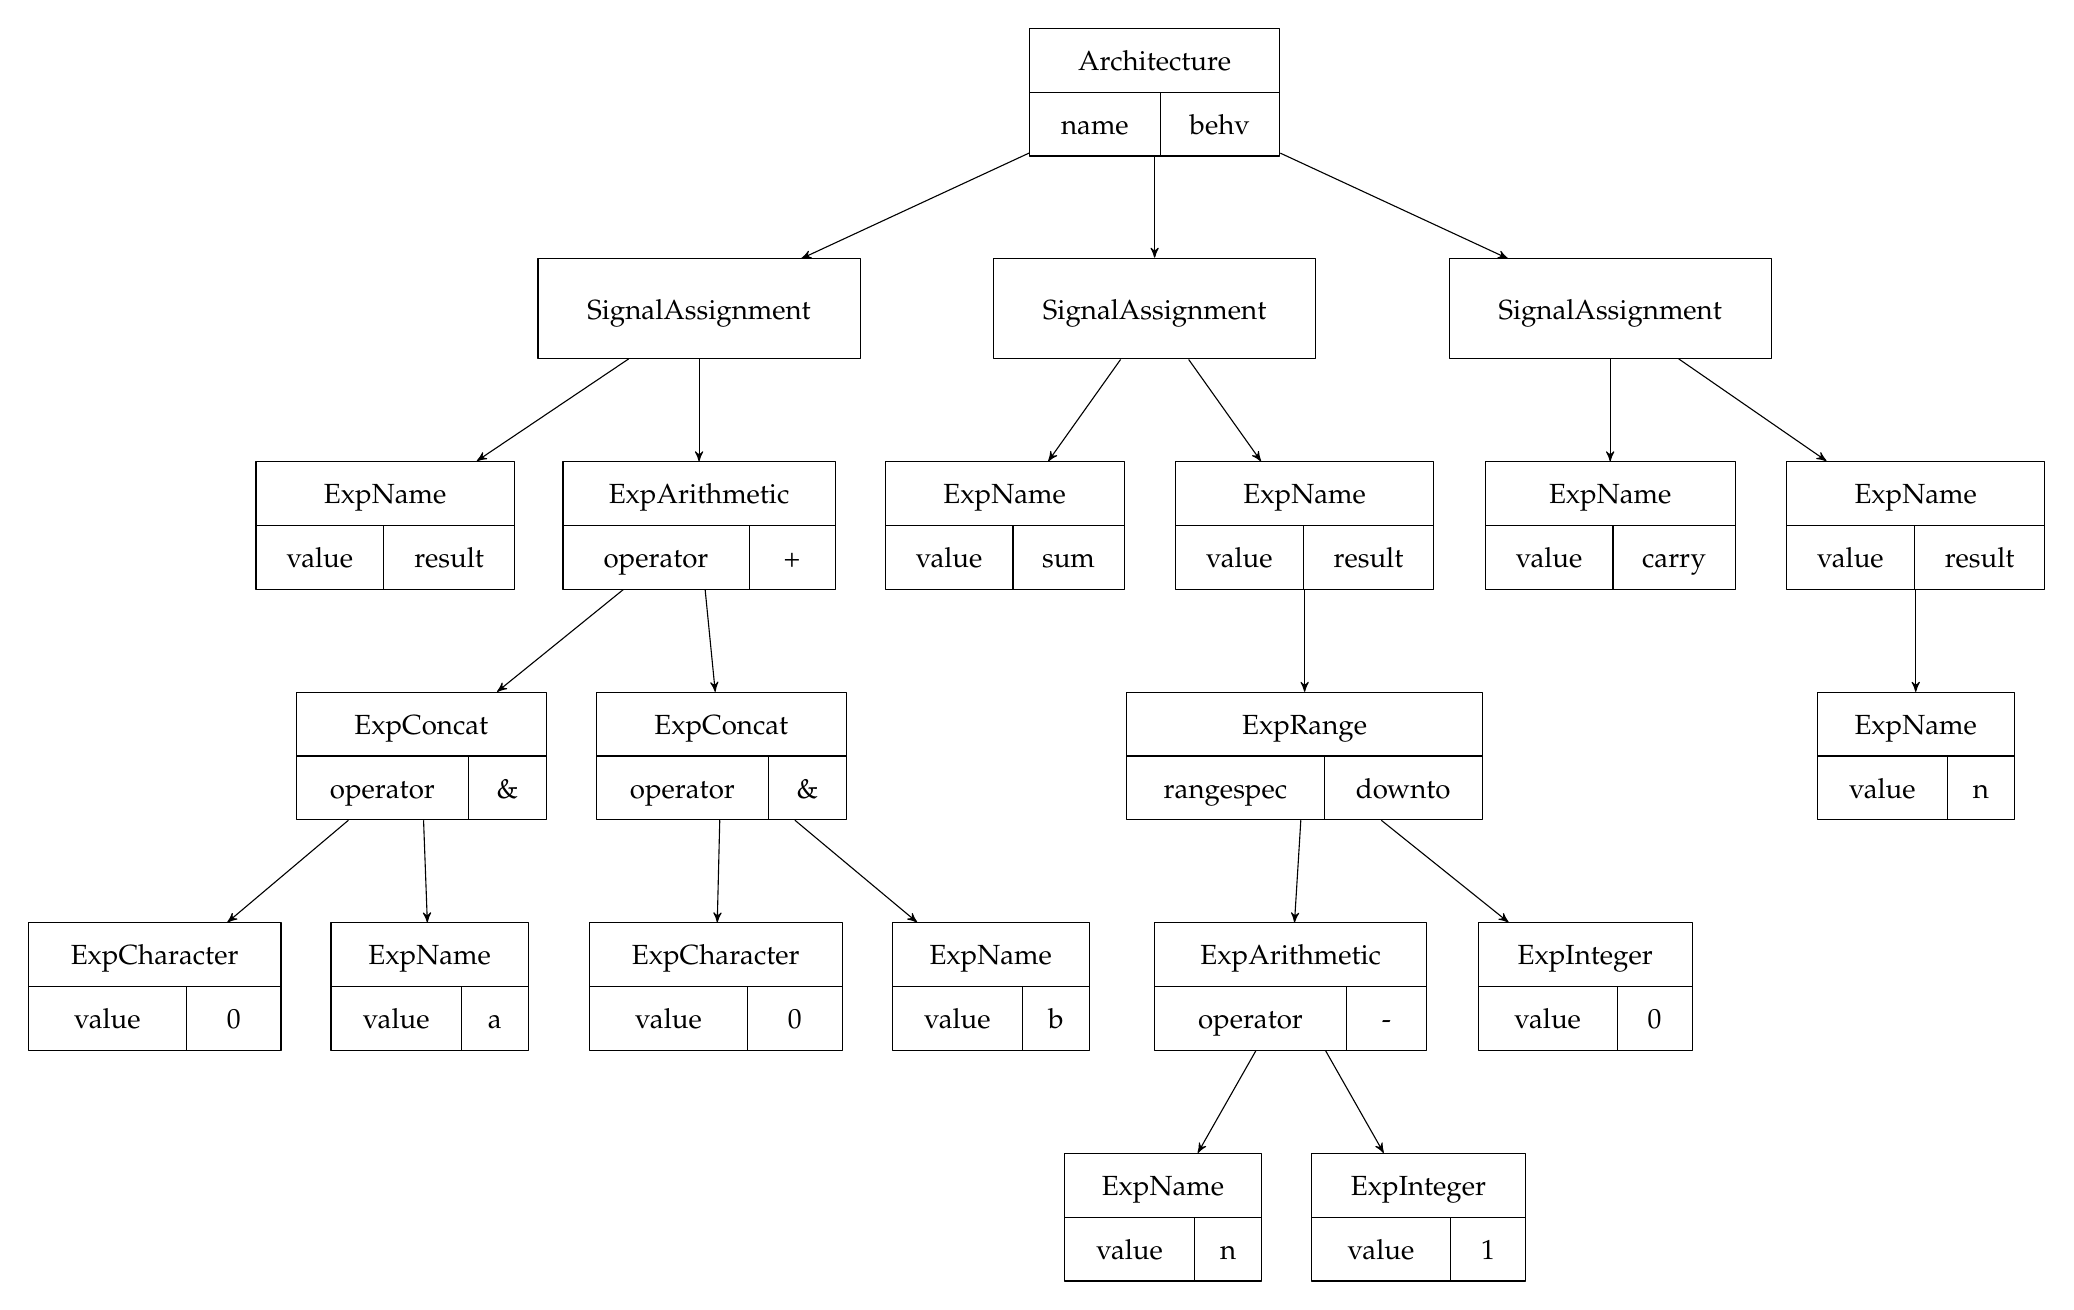
\begin{tikzpicture}[line join=bevel,anchor=base]%
\pgfsetcolor{black}
  % Edge: node_1_1 -> node_10_2
  \draw [-stealth'] (393.25bp,332.25bp) .. controls (387.28bp,323.85bp) and (379.92bp,313.5bp)  .. (367.2bp,295.59bp);
  % Edge: node_010_3 -> node_0101_4
  \draw [-stealth'] (142.32bp,166.37bp) .. controls (142.62bp,158.15bp) and (142.98bp,148.66bp)  .. (143.68bp,129.61bp);
  % Edge: node_2_1 -> node_20_2
  \draw [-stealth'] (569.5bp,332.25bp) .. controls (569.5bp,324.36bp) and (569.5bp,314.75bp)  .. (569.5bp,295.59bp);
  % Edge: node_0_1 -> node_00_2
  \draw [-stealth'] (216.14bp,332.44bp) .. controls (202.52bp,323.29bp) and (185.4bp,311.77bp)  .. (161.5bp,295.7bp);
  % Edge: node__0 -> node_1_1
  \draw [-stealth'] (405.5bp,405.11bp) .. controls (405.5bp,396.98bp) and (405.5bp,387.7bp)  .. (405.5bp,368.91bp);
  % Edge: node_1100_4 -> node_11001_5
  \draw [-stealth'] (467.07bp,83.366bp) .. controls (471.94bp,74.794bp) and (477.6bp,64.83bp)  .. (487.95bp,46.607bp);
  % Edge: node_01_2 -> node_011_3
  \draw [-stealth'] (243.69bp,249.37bp) .. controls (244.5bp,241.15bp) and (245.44bp,231.66bp)  .. (247.32bp,212.61bp);
  % Edge: node_110_3 -> node_1100_4
  \draw [-stealth'] (458.13bp,166.37bp) .. controls (457.63bp,158.15bp) and (457.04bp,148.66bp)  .. (455.86bp,129.61bp);
  % Edge: node_11_2 -> node_110_3
  \draw [-stealth'] (459.5bp,249.37bp) .. controls (459.5bp,241.15bp) and (459.5bp,231.66bp)  .. (459.5bp,212.61bp);
  % Edge: node_110_3 -> node_1101_4
  \draw [-stealth'] (487.1bp,166.37bp) .. controls (498.79bp,156.99bp) and (512.56bp,145.95bp)  .. (532.93bp,129.61bp);
  % Edge: node_2_1 -> node_21_2
  \draw [-stealth'] (594.19bp,332.44bp) .. controls (607.32bp,323.37bp) and (623.8bp,311.98bp)  .. (647.37bp,295.7bp);
  % Edge: node_1100_4 -> node_11000_5
  \draw [-stealth'] (441.93bp,83.366bp) .. controls (437.06bp,74.794bp) and (431.4bp,64.83bp)  .. (421.05bp,46.607bp);
  % Edge: node__0 -> node_0_1
  \draw [-stealth'] (360.25bp,406.53bp) .. controls (337.59bp,396.03bp) and (310.2bp,383.34bp)  .. (278.32bp,368.56bp);
  % Edge: node_01_2 -> node_010_3
  \draw [-stealth'] (214.17bp,249.37bp) .. controls (202.6bp,239.99bp) and (188.97bp,228.95bp)  .. (168.79bp,212.61bp);
  % Edge: node_011_3 -> node_0110_4
  \draw [-stealth'] (248.95bp,166.37bp) .. controls (248.75bp,158.15bp) and (248.52bp,148.66bp)  .. (248.05bp,129.61bp);
  % Edge: node_010_3 -> node_0100_4
  \draw [-stealth'] (115.27bp,166.37bp) .. controls (104.26bp,157.08bp) and (91.319bp,146.16bp)  .. (71.701bp,129.61bp);
  % Edge: node_1_1 -> node_11_2
  \draw [-stealth'] (417.75bp,332.25bp) .. controls (423.72bp,323.85bp) and (431.08bp,313.5bp)  .. (443.8bp,295.59bp);
  % Edge: node_21_2 -> node_210_3
  \draw [-stealth'] (679.5bp,249.37bp) .. controls (679.5bp,241.15bp) and (679.5bp,231.66bp)  .. (679.5bp,212.61bp);
  % Edge: node_011_3 -> node_0111_4
  \draw [-stealth'] (276.01bp,166.37bp) .. controls (287.13bp,157.08bp) and (300.2bp,146.16bp)  .. (320.03bp,129.61bp);
  % Edge: node_0_1 -> node_01_2
  \draw [-stealth'] (241.5bp,332.25bp) .. controls (241.5bp,324.36bp) and (241.5bp,314.75bp)  .. (241.5bp,295.59bp);
  % Edge: node__0 -> node_2_1
  \draw [-stealth'] (450.75bp,406.53bp) .. controls (473.41bp,396.03bp) and (500.8bp,383.34bp)  .. (532.68bp,368.56bp);
  % Node: node_0100_4
\begin{scope}
  \definecolor{strokecol}{rgb}{0.0,0.0,0.0};
  \pgfsetstrokecolor{strokecol}
  \draw (0.0bp,83.5bp) -- (0.0bp,129.5bp) -- (91.0bp,129.5bp) -- (91.0bp,83.5bp) -- cycle;
  \draw (0.0bp,106.5bp) -- (91.0bp,106.5bp);
  \draw (57.0bp,83.5bp) -- (57.0bp,106.5bp);
  \draw (45.5bp,114.3bp) node {ExpCharacter};
  \draw (28.5bp,91.3bp) node {value};
  \draw (74.0bp,91.3bp) node {0};
\end{scope}
  % Node: node_110_3
\begin{scope}
  \definecolor{strokecol}{rgb}{0.0,0.0,0.0};
  \pgfsetstrokecolor{strokecol}
  \draw (395.5bp,166.5bp) -- (395.5bp,212.5bp) -- (523.5bp,212.5bp) -- (523.5bp,166.5bp) -- cycle;
  \draw (395.5bp,189.5bp) -- (523.5bp,189.5bp);
  \draw (466.5bp,166.5bp) -- (466.5bp,189.5bp);
  \draw (459.5bp,197.3bp) node {ExpRange};
  \draw (431.0bp,174.3bp) node {rangespec};
  \draw (495.0bp,174.3bp) node {downto};
\end{scope}
  % Node: node_0101_4
\begin{scope}
  \definecolor{strokecol}{rgb}{0.0,0.0,0.0};
  \pgfsetstrokecolor{strokecol}
  \draw (109.0bp,83.5bp) -- (109.0bp,129.5bp) -- (180.0bp,129.5bp) -- (180.0bp,83.5bp) -- cycle;
  \draw (109.0bp,106.5bp) -- (180.0bp,106.5bp);
  \draw (156.0bp,83.5bp) -- (156.0bp,106.5bp);
  \draw (144.5bp,114.3bp) node {ExpName};
  \draw (132.5bp,91.3bp) node {value};
  \draw (168.0bp,91.3bp) node {a};
\end{scope}
  % Node: node_01_2
\begin{scope}
  \definecolor{strokecol}{rgb}{0.0,0.0,0.0};
  \pgfsetstrokecolor{strokecol}
  \draw (192.5bp,249.5bp) -- (192.5bp,295.5bp) -- (290.5bp,295.5bp) -- (290.5bp,249.5bp) -- cycle;
  \draw (192.5bp,272.5bp) -- (290.5bp,272.5bp);
  \draw (259.5bp,249.5bp) -- (259.5bp,272.5bp);
  \draw (241.5bp,280.3bp) node {ExpArithmetic};
  \draw (226.0bp,257.3bp) node {operator};
  \draw (275.0bp,257.3bp) node {+};
\end{scope}
  % Node: node_1101_4
\begin{scope}
  \definecolor{strokecol}{rgb}{0.0,0.0,0.0};
  \pgfsetstrokecolor{strokecol}
  \draw (522.0bp,83.5bp) -- (522.0bp,129.5bp) -- (599.0bp,129.5bp) -- (599.0bp,83.5bp) -- cycle;
  \draw (522.0bp,106.5bp) -- (599.0bp,106.5bp);
  \draw (572.0bp,83.5bp) -- (572.0bp,106.5bp);
  \draw (560.5bp,114.3bp) node {ExpInteger};
  \draw (547.0bp,91.3bp) node {value};
  \draw (585.5bp,91.3bp) node {0};
\end{scope}
  % Node: node_11001_5
\begin{scope}
  \definecolor{strokecol}{rgb}{0.0,0.0,0.0};
  \pgfsetstrokecolor{strokecol}
  \draw (462.0bp,0.5bp) -- (462.0bp,46.5bp) -- (539.0bp,46.5bp) -- (539.0bp,0.5bp) -- cycle;
  \draw (462.0bp,23.5bp) -- (539.0bp,23.5bp);
  \draw (512.0bp,0.5bp) -- (512.0bp,23.5bp);
  \draw (500.5bp,31.3bp) node {ExpInteger};
  \draw (487.0bp,8.3bp) node {value};
  \draw (525.5bp,8.3bp) node {1};
\end{scope}
  % Node: node_21_2
\begin{scope}
  \definecolor{strokecol}{rgb}{0.0,0.0,0.0};
  \pgfsetstrokecolor{strokecol}
  \draw (633.0bp,249.5bp) -- (633.0bp,295.5bp) -- (726.0bp,295.5bp) -- (726.0bp,249.5bp) -- cycle;
  \draw (633.0bp,272.5bp) -- (726.0bp,272.5bp);
  \draw (679.0bp,249.5bp) -- (679.0bp,272.5bp);
  \draw (679.5bp,280.3bp) node {ExpName};
  \draw (656.0bp,257.3bp) node {value};
  \draw (702.5bp,257.3bp) node {result};
\end{scope}
  % Node: node_11000_5
\begin{scope}
  \definecolor{strokecol}{rgb}{0.0,0.0,0.0};
  \pgfsetstrokecolor{strokecol}
  \draw (373.0bp,0.5bp) -- (373.0bp,46.5bp) -- (444.0bp,46.5bp) -- (444.0bp,0.5bp) -- cycle;
  \draw (373.0bp,23.5bp) -- (444.0bp,23.5bp);
  \draw (420.0bp,0.5bp) -- (420.0bp,23.5bp);
  \draw (408.5bp,31.3bp) node {ExpName};
  \draw (396.5bp,8.3bp) node {value};
  \draw (432.0bp,8.3bp) node {n};
\end{scope}
  % Node: node_20_2
\begin{scope}
  \definecolor{strokecol}{rgb}{0.0,0.0,0.0};
  \pgfsetstrokecolor{strokecol}
  \draw (524.5bp,249.5bp) -- (524.5bp,295.5bp) -- (614.5bp,295.5bp) -- (614.5bp,249.5bp) -- cycle;
  \draw (524.5bp,272.5bp) -- (614.5bp,272.5bp);
  \draw (570.5bp,249.5bp) -- (570.5bp,272.5bp);
  \draw (569.5bp,280.3bp) node {ExpName};
  \draw (547.5bp,257.3bp) node {value};
  \draw (592.5bp,257.3bp) node {carry};
\end{scope}
  % Node: node_2_1
\begin{scope}
  \definecolor{strokecol}{rgb}{0.0,0.0,0.0};
  \pgfsetstrokecolor{strokecol}
  \draw (511.5bp,332.5bp) -- (511.5bp,368.5bp) -- (627.5bp,368.5bp) -- (627.5bp,332.5bp) -- cycle;
  \draw (569.5bp,346.8bp) node {SignalAssignment};
\end{scope}
  % Node: node__0
\begin{scope}
  \definecolor{strokecol}{rgb}{0.0,0.0,0.0};
  \pgfsetstrokecolor{strokecol}
  \draw (360.5bp,405.5bp) -- (360.5bp,451.5bp) -- (450.5bp,451.5bp) -- (450.5bp,405.5bp) -- cycle;
  \draw (360.5bp,428.5bp) -- (450.5bp,428.5bp);
  \draw (407.5bp,405.5bp) -- (407.5bp,428.5bp);
  \draw (405.5bp,436.3bp) node {Architecture};
  \draw (384.0bp,413.3bp) node {name};
  \draw (429.0bp,413.3bp) node {behv};
\end{scope}
  % Node: node_10_2
\begin{scope}
  \definecolor{strokecol}{rgb}{0.0,0.0,0.0};
  \pgfsetstrokecolor{strokecol}
  \draw (308.5bp,249.5bp) -- (308.5bp,295.5bp) -- (394.5bp,295.5bp) -- (394.5bp,249.5bp) -- cycle;
  \draw (308.5bp,272.5bp) -- (394.5bp,272.5bp);
  \draw (354.5bp,249.5bp) -- (354.5bp,272.5bp);
  \draw (351.5bp,280.3bp) node {ExpName};
  \draw (331.5bp,257.3bp) node {value};
  \draw (374.5bp,257.3bp) node {sum};
\end{scope}
  % Node: node_11_2
\begin{scope}
  \definecolor{strokecol}{rgb}{0.0,0.0,0.0};
  \pgfsetstrokecolor{strokecol}
  \draw (413.0bp,249.5bp) -- (413.0bp,295.5bp) -- (506.0bp,295.5bp) -- (506.0bp,249.5bp) -- cycle;
  \draw (413.0bp,272.5bp) -- (506.0bp,272.5bp);
  \draw (459.0bp,249.5bp) -- (459.0bp,272.5bp);
  \draw (459.5bp,280.3bp) node {ExpName};
  \draw (436.0bp,257.3bp) node {value};
  \draw (482.5bp,257.3bp) node {result};
\end{scope}
  % Node: node_0111_4
\begin{scope}
  \definecolor{strokecol}{rgb}{0.0,0.0,0.0};
  \pgfsetstrokecolor{strokecol}
  \draw (311.0bp,83.5bp) -- (311.0bp,129.5bp) -- (382.0bp,129.5bp) -- (382.0bp,83.5bp) -- cycle;
  \draw (311.0bp,106.5bp) -- (382.0bp,106.5bp);
  \draw (358.0bp,83.5bp) -- (358.0bp,106.5bp);
  \draw (346.5bp,114.3bp) node {ExpName};
  \draw (334.5bp,91.3bp) node {value};
  \draw (370.0bp,91.3bp) node {b};
\end{scope}
  % Node: node_00_2
\begin{scope}
  \definecolor{strokecol}{rgb}{0.0,0.0,0.0};
  \pgfsetstrokecolor{strokecol}
  \draw (82.0bp,249.5bp) -- (82.0bp,295.5bp) -- (175.0bp,295.5bp) -- (175.0bp,249.5bp) -- cycle;
  \draw (82.0bp,272.5bp) -- (175.0bp,272.5bp);
  \draw (128.0bp,249.5bp) -- (128.0bp,272.5bp);
  \draw (128.5bp,280.3bp) node {ExpName};
  \draw (105.0bp,257.3bp) node {value};
  \draw (151.5bp,257.3bp) node {result};
\end{scope}
  % Node: node_1100_4
\begin{scope}
  \definecolor{strokecol}{rgb}{0.0,0.0,0.0};
  \pgfsetstrokecolor{strokecol}
  \draw (405.5bp,83.5bp) -- (405.5bp,129.5bp) -- (503.5bp,129.5bp) -- (503.5bp,83.5bp) -- cycle;
  \draw (405.5bp,106.5bp) -- (503.5bp,106.5bp);
  \draw (474.5bp,83.5bp) -- (474.5bp,106.5bp);
  \draw (454.5bp,114.3bp) node {ExpArithmetic};
  \draw (440.0bp,91.3bp) node {operator};
  \draw (489.0bp,91.3bp) node {-};
\end{scope}
  % Node: node_210_3
\begin{scope}
  \definecolor{strokecol}{rgb}{0.0,0.0,0.0};
  \pgfsetstrokecolor{strokecol}
  \draw (644.0bp,166.5bp) -- (644.0bp,212.5bp) -- (715.0bp,212.5bp) -- (715.0bp,166.5bp) -- cycle;
  \draw (644.0bp,189.5bp) -- (715.0bp,189.5bp);
  \draw (691.0bp,166.5bp) -- (691.0bp,189.5bp);
  \draw (679.5bp,197.3bp) node {ExpName};
  \draw (667.5bp,174.3bp) node {value};
  \draw (703.0bp,174.3bp) node {n};
\end{scope}
  % Node: node_010_3
\begin{scope}
  \definecolor{strokecol}{rgb}{0.0,0.0,0.0};
  \pgfsetstrokecolor{strokecol}
  \draw (96.5bp,166.5bp) -- (96.5bp,212.5bp) -- (186.5bp,212.5bp) -- (186.5bp,166.5bp) -- cycle;
  \draw (96.5bp,189.5bp) -- (186.5bp,189.5bp);
  \draw (158.5bp,166.5bp) -- (158.5bp,189.5bp);
  \draw (141.5bp,197.3bp) node {ExpConcat};
  \draw (127.5bp,174.3bp) node {operator};
  \draw (172.5bp,174.3bp) node {\&};
\end{scope}
  % Node: node_0110_4
\begin{scope}
  \definecolor{strokecol}{rgb}{0.0,0.0,0.0};
  \pgfsetstrokecolor{strokecol}
  \draw (202.0bp,83.5bp) -- (202.0bp,129.5bp) -- (293.0bp,129.5bp) -- (293.0bp,83.5bp) -- cycle;
  \draw (202.0bp,106.5bp) -- (293.0bp,106.5bp);
  \draw (259.0bp,83.5bp) -- (259.0bp,106.5bp);
  \draw (247.5bp,114.3bp) node {ExpCharacter};
  \draw (230.5bp,91.3bp) node {value};
  \draw (276.0bp,91.3bp) node {0};
\end{scope}
  % Node: node_1_1
\begin{scope}
  \definecolor{strokecol}{rgb}{0.0,0.0,0.0};
  \pgfsetstrokecolor{strokecol}
  \draw (347.5bp,332.5bp) -- (347.5bp,368.5bp) -- (463.5bp,368.5bp) -- (463.5bp,332.5bp) -- cycle;
  \draw (405.5bp,346.8bp) node {SignalAssignment};
\end{scope}
  % Node: node_011_3
\begin{scope}
  \definecolor{strokecol}{rgb}{0.0,0.0,0.0};
  \pgfsetstrokecolor{strokecol}
  \draw (204.5bp,166.5bp) -- (204.5bp,212.5bp) -- (294.5bp,212.5bp) -- (294.5bp,166.5bp) -- cycle;
  \draw (204.5bp,189.5bp) -- (294.5bp,189.5bp);
  \draw (266.5bp,166.5bp) -- (266.5bp,189.5bp);
  \draw (249.5bp,197.3bp) node {ExpConcat};
  \draw (235.5bp,174.3bp) node {operator};
  \draw (280.5bp,174.3bp) node {\&};
\end{scope}
  % Node: node_0_1
\begin{scope}
  \definecolor{strokecol}{rgb}{0.0,0.0,0.0};
  \pgfsetstrokecolor{strokecol}
  \draw (183.5bp,332.5bp) -- (183.5bp,368.5bp) -- (299.5bp,368.5bp) -- (299.5bp,332.5bp) -- cycle;
  \draw (241.5bp,346.8bp) node {SignalAssignment};
\end{scope}
\end{tikzpicture}}%

    \caption{An example graph generated by Yodl}
    \label{fig:simpleAdder}
\end{figure}

\noindent The implementation splits the problem into three major parts:
\begin{enumerate}
    \item Extraction of the relevant information from the AST into an
    intermediate format
    \item Modification of the resulting data for better processing
    \item Traversal and code generation
\end{enumerate}

\subsubsection{Extraction of information from the AST}
After parsing has
finished, the complete information from the original VHDL source code
lies in the AST. This data structure is built from objects
representing expressions, signal assignments or control
structures. The current data model, for reference, defines an
ExpArithmetic object like the following:
%
\begin{lstlisting}[style=c++]
class Expression { /* Abstract base class for expressions */ };

class ExpBinary : public Expression {
public:
    ExpBinary(Expression *op1, Expression *op2);
    /* Intentionally left out */

public:
    Expression *operand1_;
    Expression *operand2_;
};

class ExpArithmetic : public ExpBinary {
public:
    enum fun_t {PLUS, MINUS, MULT, DIV, MOD, REM, POW, xCONCAT};
    ExpArithmetic(ExpArithmetic::fun_t op, Expression *op1, Expression *op2);
    /* Intentionally left out */

public:
    fun_t fun_;
}
\end{lstlisting}
%
This depiction is heavily simplified and does not comprehensively
represent all details of ExpArithmetic objects. Objects that represent
whole \VH{Architectures} are obviously even more complicated. The
class definition of an \VH{Architecture} object contains the name of
the architecture, a linked list of concurrent statements and all
possible declarations that can occur in the architecture header.

In order to extract the mentioned information from the AST, each node
(= object) has to be visited. In OOP, there generally are two possible
solutions for this kind of traversal. On the one hand, every node
object of the AST could implement a virtual method that outputs the
desired information in a special data structure. On the other hand,
the AST could completely be traversed from outside. However, the
second option clearly imposes the public member access upon all member
variables of the objects. Within the scope of this work, the first
solution has been implemented and shall now be elaborated.

As mentioned before, the first step produces data in some kind of
intermediate format. Since the AST itself is an n-ary tree, the output
ought to be a tree as well. For this purpose, the class
\emph{SimpleTree} has been introduced. Its class declaration shall be
given in the following listing.
%
\begin{lstlisting}[style=c++]
class SimpleTree {
public:
    SimpleTree(const std::map<string, string> s) : root(s) { };
    SimpleTree(const map<string, string> s,
               std::vector<SimpleTree<std::map<string,string>>*> own)
        : root(s), forest(own) { };
    /* further ctor and dtor declarations intentionally left out */
public:
    std::map<string, string> root;
    std::vector<SimpleTree<std::map<string, string>>*> forest;
};
\end{lstlisting}
%
Note, that the original class uses C++-Templates but, due to the great
negative influence of templates on the readability, an instantiated
version of the class was printed. As the code shows, the data type
used for this instantiation is \CPP{std::map<string, string>}.

In order to visualize the runtime structure of a \CPP{SimpleTree}
tree, an example is given in figure \ref{fig:simpletree}.
%
\begin{figure}[tb]
    \centering
    \caption{Runtime structure of a SimpleTree oject}
    \resizebox{\textwidth}{!}{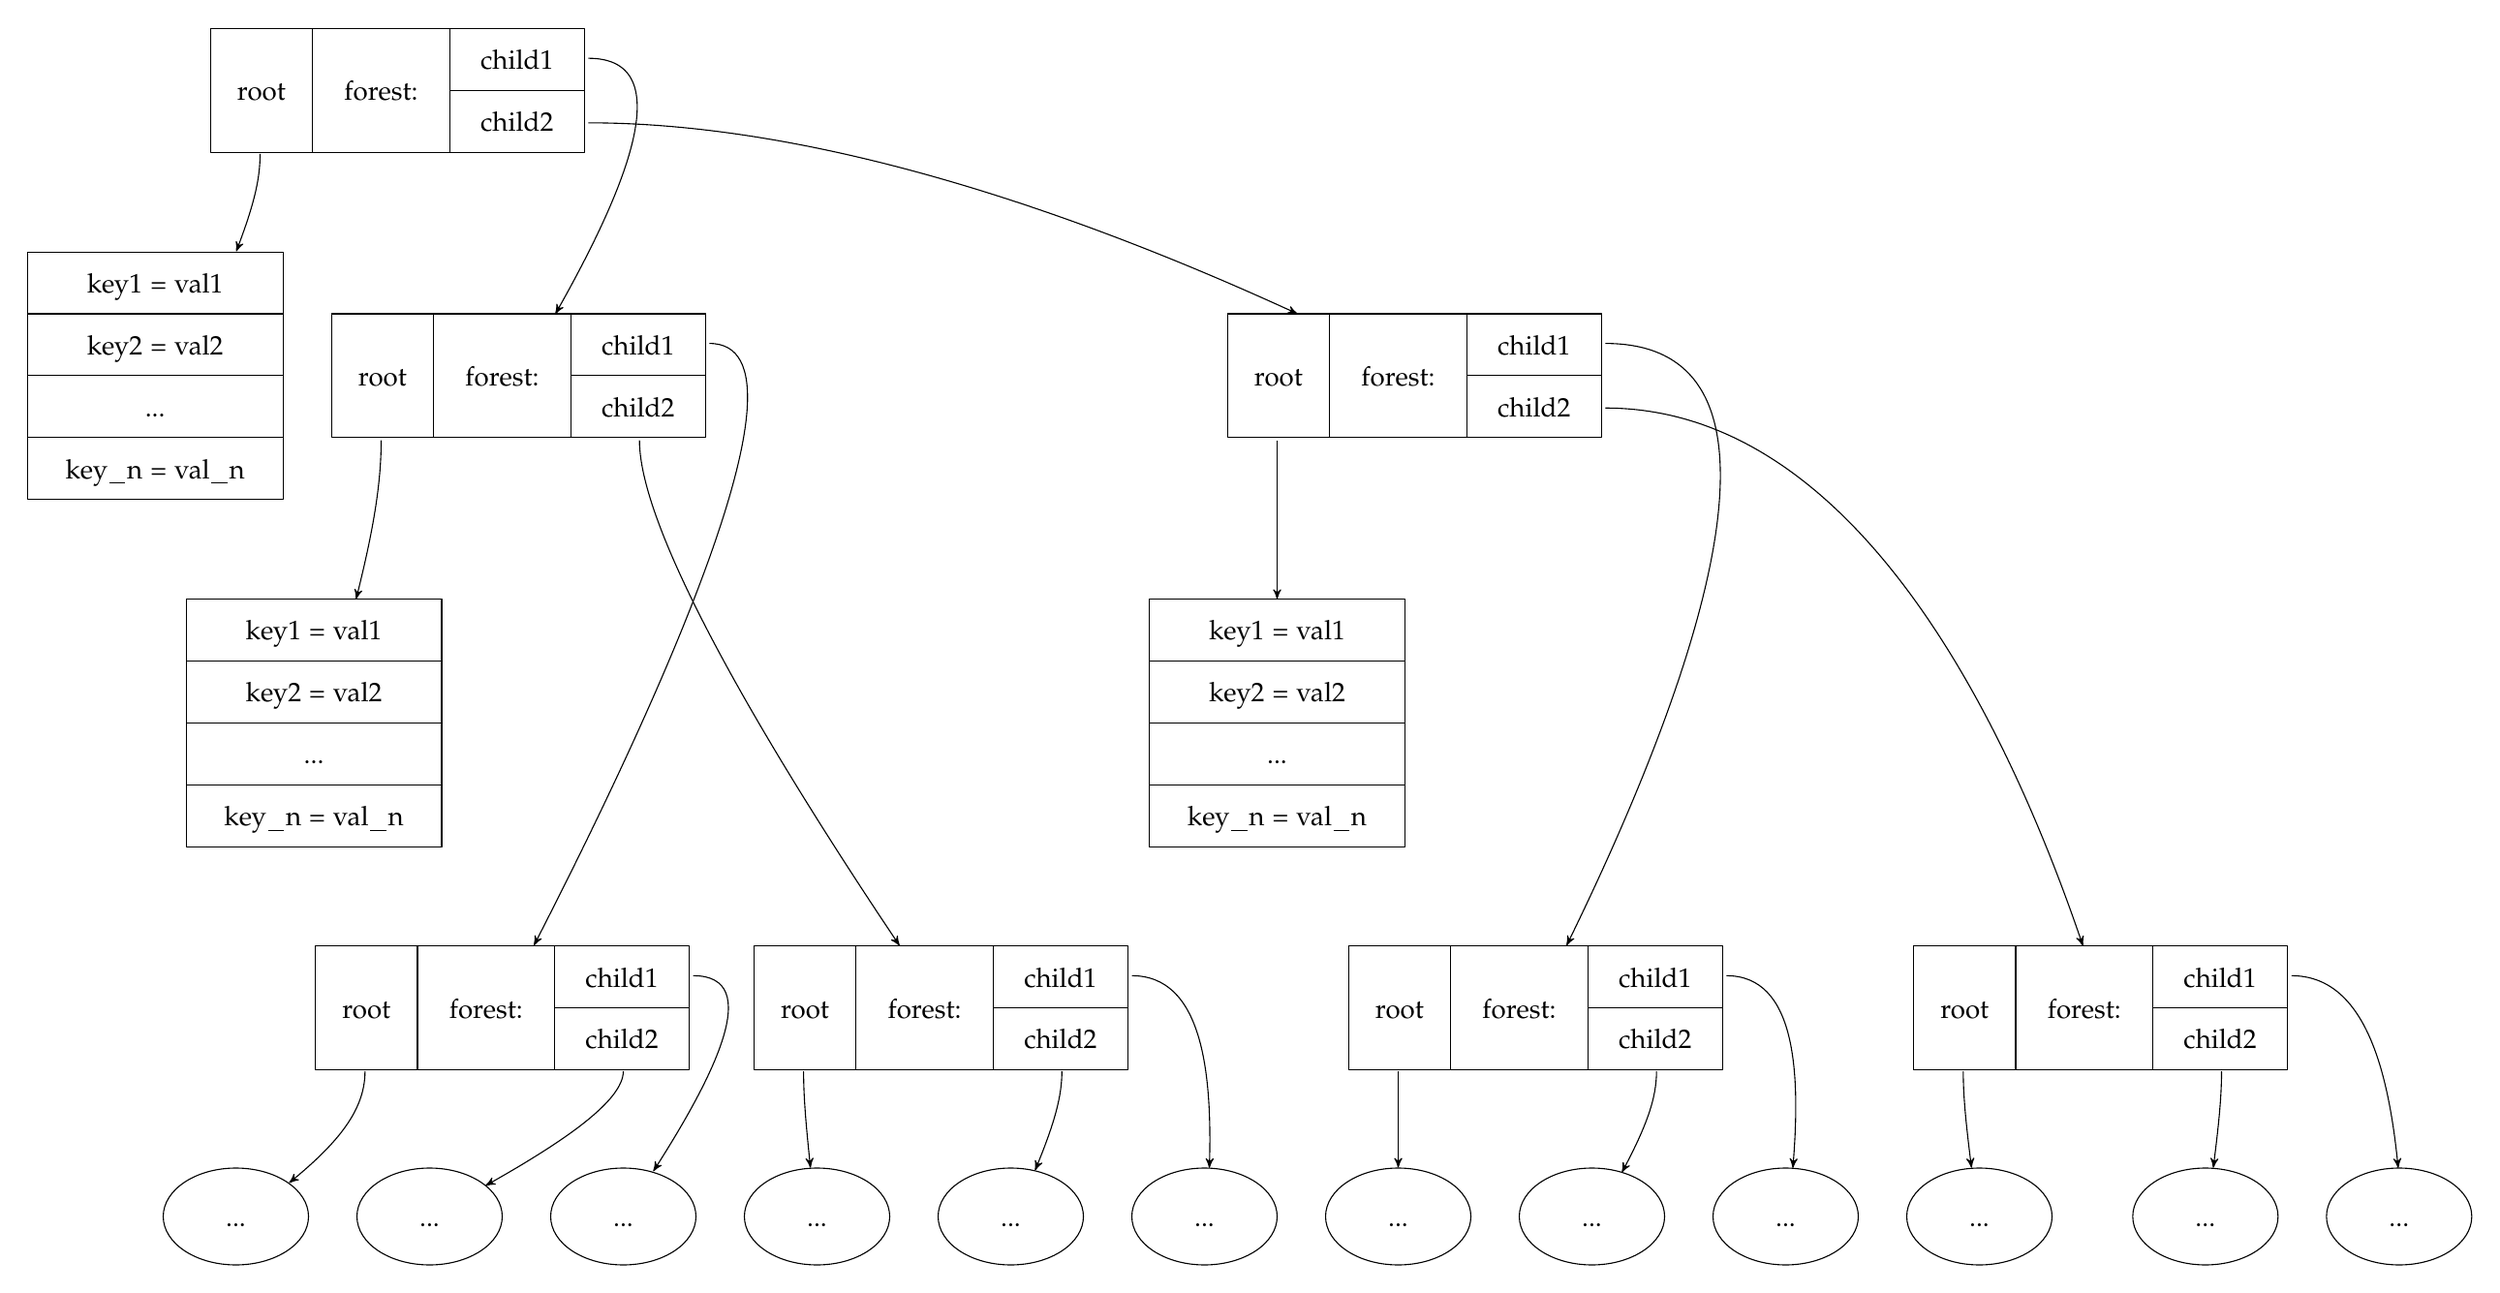
\begin{tikzpicture}[line join=bevel,anchor=base]%
\begin{scope}
  \pgfsetstrokecolor{black}
  \definecolor{strokecol}{rgb}{1.0,1.0,1.0};
  \pgfsetstrokecolor{strokecol}
  \definecolor{fillcol}{rgb}{1.0,1.0,1.0};
  \pgfsetfillcolor{fillcol}
  \filldraw (0.0bp,0.0bp) -- (0.0bp,460.0bp) -- (908.5bp,460.0bp) -- (908.5bp,0.0bp) -- cycle;
\end{scope}
\begin{scope}
  \pgfsetstrokecolor{black}
  \definecolor{strokecol}{rgb}{1.0,1.0,1.0};
  \pgfsetstrokecolor{strokecol}
  \definecolor{fillcol}{rgb}{1.0,1.0,1.0};
  \pgfsetfillcolor{fillcol}
  \filldraw (0.0bp,0.0bp) -- (0.0bp,460.0bp) -- (908.5bp,460.0bp) -- (908.5bp,0.0bp) -- cycle;
\end{scope}
  \pgfsetcolor{black}
  % Edge: child22 -> dots4
  \draw [-stealth'] (719.5bp,72.0bp) .. controls (719.5bp,63.536bp) and (720.26bp,54.359bp)  .. (722.57bp,36.13bp);
  % Edge: child12 -> dots2
  \draw [-stealth'] (288.5bp,72.0bp) .. controls (288.5bp,63.646bp) and (289.12bp,54.584bp)  .. (291.06bp,36.147bp);
  % Edge: child21 -> dots3
  \draw [-stealth'] (509.5bp,72.0bp) .. controls (509.5bp,63.683bp) and (509.5bp,54.631bp)  .. (509.5bp,36.186bp);
  % Edge: child2 -> mapChild2
  \draw [-stealth'] (464.5bp,306.5bp) .. controls (464.5bp,290.65bp) and (464.5bp,273.45bp)  .. (464.5bp,247.55bp);
  % Edge: child22 -> dotsn8
  \draw [-stealth'] (815.5bp,72.0bp) .. controls (815.5bp,63.536bp) and (814.74bp,54.359bp)  .. (812.43bp,36.13bp);
  % Edge: child21 -> dotsn6
  \draw [-stealth'] (605.5bp,72.0bp) .. controls (605.5bp,62.06bp) and (601.95bp,51.931bp)  .. (592.66bp,34.416bp);
  % Edge: child11 -> dots1
  \draw [-stealth'] (125.5bp,72.0bp) .. controls (125.5bp,57.854bp) and (115.99bp,45.8bp)  .. (97.301bp,30.487bp);
  % Edge: child1 -> child11
  \draw [-stealth'] (253.5bp,342.5bp) .. controls (297.97bp,342.5bp) and (227.0bp,194.26bp)  .. (188.29bp,118.76bp);
  % Edge: root -> mapRoot
  \draw [-stealth'] (86.5bp,413.0bp) .. controls (86.5bp,403.9bp) and (84.497bp,394.74bp)  .. (77.65bp,376.73bp);
  % Edge: root -> child1
  \draw [-stealth'] (208.5bp,448.5bp) .. controls (243.84bp,448.5bp) and (220.85bp,397.01bp)  .. (196.27bp,353.51bp);
  % Edge: child22 -> dotsn7
  \draw [-stealth'] (841.5bp,107.5bp) .. controls (868.77bp,107.5bp) and (877.55bp,72.183bp)  .. (881.15bp,36.064bp);
  % Edge: child12 -> dotsn3
  \draw [-stealth'] (410.5bp,107.5bp) .. controls (436.48bp,107.5bp) and (440.41bp,72.183bp)  .. (439.31bp,36.064bp);
  % Edge: root -> child2
  \draw [-stealth'] (208.5bp,424.5bp) .. controls (301.01bp,424.5bp) and (402.72bp,385.34bp)  .. (472.02bp,353.54bp);
  % Edge: child11 -> dotsn2
  \draw [-stealth'] (221.5bp,72.0bp) .. controls (221.5bp,60.895bp) and (199.01bp,45.647bp)  .. (170.33bp,29.476bp);
  % Edge: child2 -> child22
  \draw [-stealth'] (586.5bp,318.5bp) .. controls (684.18bp,318.5bp) and (739.86bp,189.51bp)  .. (763.99bp,118.6bp);
  % Edge: child21 -> dotsn5
  \draw [-stealth'] (631.5bp,107.5bp) .. controls (657.1bp,107.5bp) and (659.14bp,72.183bp)  .. (656.17bp,36.064bp);
  % Edge: child12 -> dotsn4
  \draw [-stealth'] (384.5bp,72.0bp) .. controls (384.5bp,62.726bp) and (381.89bp,53.047bp)  .. (374.55bp,35.177bp);
  % Edge: child1 -> mapChild1
  \draw [-stealth'] (131.5bp,306.5bp) .. controls (131.5bp,290.35bp) and (128.62bp,273.18bp)  .. (122.19bp,247.5bp);
  % Edge: child1 -> child12
  \draw [-stealth'] (227.5bp,306.5bp) .. controls (227.5bp,268.28bp) and (285.98bp,175.64bp)  .. (324.16bp,118.68bp);
  % Edge: child11 -> dotsn1
  \draw [-stealth'] (247.5bp,107.5bp) .. controls (274.29bp,107.5bp) and (254.97bp,69.713bp)  .. (232.67bp,34.822bp);
  % Edge: child2 -> child21
  \draw [-stealth'] (586.5bp,342.5bp) .. controls (671.85bp,342.5bp) and (609.02bp,194.26bp)  .. (572.1bp,118.76bp);
  % Node: child1
\begin{scope}
  \definecolor{strokecol}{rgb}{0.0,0.0,0.0};
  \pgfsetstrokecolor{strokecol}
  \draw (113.0bp,307.5bp) -- (113.0bp,353.5bp) -- (252.0bp,353.5bp) -- (252.0bp,307.5bp) -- cycle;
  \draw (151.0bp,307.5bp) -- (151.0bp,353.5bp);
  \draw (202.0bp,307.5bp) -- (202.0bp,353.5bp);
  \draw (202.0bp,330.5bp) -- (252.0bp,330.5bp);
  \draw (132.0bp,326.8bp) node {root};
  \draw (176.5bp,326.8bp) node {forest:};
  \draw (227.0bp,338.3bp) node {child1};
  \draw (227.0bp,315.3bp) node {child2};
\end{scope}
  % Node: mapChild1
\begin{scope}
  \definecolor{strokecol}{rgb}{0.0,0.0,0.0};
  \pgfsetstrokecolor{strokecol}
  \draw (59.0bp,155.5bp) -- (59.0bp,247.5bp) -- (154.0bp,247.5bp) -- (154.0bp,155.5bp) -- cycle;
  \draw (59.0bp,224.5bp) -- (154.0bp,224.5bp);
  \draw (59.0bp,201.5bp) -- (154.0bp,201.5bp);
  \draw (59.0bp,178.5bp) -- (154.0bp,178.5bp);
  \draw (106.5bp,232.3bp) node {key1 = val1};
  \draw (106.5bp,209.3bp) node {key2 = val2};
  \draw (106.5bp,186.3bp) node {...};
  \draw (106.5bp,163.3bp) node {key_n = val_n};
\end{scope}
  % Node: mapChild2
\begin{scope}
  \definecolor{strokecol}{rgb}{0.0,0.0,0.0};
  \pgfsetstrokecolor{strokecol}
  \draw (417.0bp,155.5bp) -- (417.0bp,247.5bp) -- (512.0bp,247.5bp) -- (512.0bp,155.5bp) -- cycle;
  \draw (417.0bp,224.5bp) -- (512.0bp,224.5bp);
  \draw (417.0bp,201.5bp) -- (512.0bp,201.5bp);
  \draw (417.0bp,178.5bp) -- (512.0bp,178.5bp);
  \draw (464.5bp,232.3bp) node {key1 = val1};
  \draw (464.5bp,209.3bp) node {key2 = val2};
  \draw (464.5bp,186.3bp) node {...};
  \draw (464.5bp,163.3bp) node {key_n = val_n};
\end{scope}
  % Node: child11
\begin{scope}
  \definecolor{strokecol}{rgb}{0.0,0.0,0.0};
  \pgfsetstrokecolor{strokecol}
  \draw (107.0bp,72.5bp) -- (107.0bp,118.5bp) -- (246.0bp,118.5bp) -- (246.0bp,72.5bp) -- cycle;
  \draw (145.0bp,72.5bp) -- (145.0bp,118.5bp);
  \draw (196.0bp,72.5bp) -- (196.0bp,118.5bp);
  \draw (196.0bp,95.5bp) -- (246.0bp,95.5bp);
  \draw (126.0bp,91.8bp) node {root};
  \draw (170.5bp,91.8bp) node {forest:};
  \draw (221.0bp,103.3bp) node {child1};
  \draw (221.0bp,80.3bp) node {child2};
\end{scope}
  % Node: child12
\begin{scope}
  \definecolor{strokecol}{rgb}{0.0,0.0,0.0};
  \pgfsetstrokecolor{strokecol}
  \draw (270.0bp,72.5bp) -- (270.0bp,118.5bp) -- (409.0bp,118.5bp) -- (409.0bp,72.5bp) -- cycle;
  \draw (308.0bp,72.5bp) -- (308.0bp,118.5bp);
  \draw (359.0bp,72.5bp) -- (359.0bp,118.5bp);
  \draw (359.0bp,95.5bp) -- (409.0bp,95.5bp);
  \draw (289.0bp,91.8bp) node {root};
  \draw (333.5bp,91.8bp) node {forest:};
  \draw (384.0bp,103.3bp) node {child1};
  \draw (384.0bp,80.3bp) node {child2};
\end{scope}
  % Node: child2
\begin{scope}
  \definecolor{strokecol}{rgb}{0.0,0.0,0.0};
  \pgfsetstrokecolor{strokecol}
  \draw (446.0bp,307.5bp) -- (446.0bp,353.5bp) -- (585.0bp,353.5bp) -- (585.0bp,307.5bp) -- cycle;
  \draw (484.0bp,307.5bp) -- (484.0bp,353.5bp);
  \draw (535.0bp,307.5bp) -- (535.0bp,353.5bp);
  \draw (535.0bp,330.5bp) -- (585.0bp,330.5bp);
  \draw (465.0bp,326.8bp) node {root};
  \draw (509.5bp,326.8bp) node {forest:};
  \draw (560.0bp,338.3bp) node {child1};
  \draw (560.0bp,315.3bp) node {child2};
\end{scope}
  % Node: dotsn1
\begin{scope}
  \definecolor{strokecol}{rgb}{0.0,0.0,0.0};
  \pgfsetstrokecolor{strokecol}
  \draw (221.5bp,18.0bp) ellipse (27.0bp and 18.0bp);
  \draw (221.5bp,14.3bp) node {...};
\end{scope}
  % Node: dotsn2
\begin{scope}
  \definecolor{strokecol}{rgb}{0.0,0.0,0.0};
  \pgfsetstrokecolor{strokecol}
  \draw (149.5bp,18.0bp) ellipse (27.0bp and 18.0bp);
  \draw (149.5bp,14.3bp) node {...};
\end{scope}
  % Node: dotsn3
\begin{scope}
  \definecolor{strokecol}{rgb}{0.0,0.0,0.0};
  \pgfsetstrokecolor{strokecol}
  \draw (437.5bp,18.0bp) ellipse (27.0bp and 18.0bp);
  \draw (437.5bp,14.3bp) node {...};
\end{scope}
  % Node: dotsn4
\begin{scope}
  \definecolor{strokecol}{rgb}{0.0,0.0,0.0};
  \pgfsetstrokecolor{strokecol}
  \draw (365.5bp,18.0bp) ellipse (27.0bp and 18.0bp);
  \draw (365.5bp,14.3bp) node {...};
\end{scope}
  % Node: dotsn5
\begin{scope}
  \definecolor{strokecol}{rgb}{0.0,0.0,0.0};
  \pgfsetstrokecolor{strokecol}
  \draw (653.5bp,18.0bp) ellipse (27.0bp and 18.0bp);
  \draw (653.5bp,14.3bp) node {...};
\end{scope}
  % Node: dotsn6
\begin{scope}
  \definecolor{strokecol}{rgb}{0.0,0.0,0.0};
  \pgfsetstrokecolor{strokecol}
  \draw (581.5bp,18.0bp) ellipse (27.0bp and 18.0bp);
  \draw (581.5bp,14.3bp) node {...};
\end{scope}
  % Node: dotsn7
\begin{scope}
  \definecolor{strokecol}{rgb}{0.0,0.0,0.0};
  \pgfsetstrokecolor{strokecol}
  \draw (881.5bp,18.0bp) ellipse (27.0bp and 18.0bp);
  \draw (881.5bp,14.3bp) node {...};
\end{scope}
  % Node: dotsn8
\begin{scope}
  \definecolor{strokecol}{rgb}{0.0,0.0,0.0};
  \pgfsetstrokecolor{strokecol}
  \draw (809.5bp,18.0bp) ellipse (27.0bp and 18.0bp);
  \draw (809.5bp,14.3bp) node {...};
\end{scope}
  % Node: dots3
\begin{scope}
  \definecolor{strokecol}{rgb}{0.0,0.0,0.0};
  \pgfsetstrokecolor{strokecol}
  \draw (509.5bp,18.0bp) ellipse (27.0bp and 18.0bp);
  \draw (509.5bp,14.3bp) node {...};
\end{scope}
  % Node: mapRoot
\begin{scope}
  \definecolor{strokecol}{rgb}{0.0,0.0,0.0};
  \pgfsetstrokecolor{strokecol}
  \draw (0.0bp,284.5bp) -- (0.0bp,376.5bp) -- (95.0bp,376.5bp) -- (95.0bp,284.5bp) -- cycle;
  \draw (0.0bp,353.5bp) -- (95.0bp,353.5bp);
  \draw (0.0bp,330.5bp) -- (95.0bp,330.5bp);
  \draw (0.0bp,307.5bp) -- (95.0bp,307.5bp);
  \draw (47.5bp,361.3bp) node {key1 = val1};
  \draw (47.5bp,338.3bp) node {key2 = val2};
  \draw (47.5bp,315.3bp) node {...};
  \draw (47.5bp,292.3bp) node {key_n = val_n};
\end{scope}
  % Node: dots1
\begin{scope}
  \definecolor{strokecol}{rgb}{0.0,0.0,0.0};
  \pgfsetstrokecolor{strokecol}
  \draw (77.5bp,18.0bp) ellipse (27.0bp and 18.0bp);
  \draw (77.5bp,14.3bp) node {...};
\end{scope}
  % Node: child22
\begin{scope}
  \definecolor{strokecol}{rgb}{0.0,0.0,0.0};
  \pgfsetstrokecolor{strokecol}
  \draw (701.0bp,72.5bp) -- (701.0bp,118.5bp) -- (840.0bp,118.5bp) -- (840.0bp,72.5bp) -- cycle;
  \draw (739.0bp,72.5bp) -- (739.0bp,118.5bp);
  \draw (790.0bp,72.5bp) -- (790.0bp,118.5bp);
  \draw (790.0bp,95.5bp) -- (840.0bp,95.5bp);
  \draw (720.0bp,91.8bp) node {root};
  \draw (764.5bp,91.8bp) node {forest:};
  \draw (815.0bp,103.3bp) node {child1};
  \draw (815.0bp,80.3bp) node {child2};
\end{scope}
  % Node: child21
\begin{scope}
  \definecolor{strokecol}{rgb}{0.0,0.0,0.0};
  \pgfsetstrokecolor{strokecol}
  \draw (491.0bp,72.5bp) -- (491.0bp,118.5bp) -- (630.0bp,118.5bp) -- (630.0bp,72.5bp) -- cycle;
  \draw (529.0bp,72.5bp) -- (529.0bp,118.5bp);
  \draw (580.0bp,72.5bp) -- (580.0bp,118.5bp);
  \draw (580.0bp,95.5bp) -- (630.0bp,95.5bp);
  \draw (510.0bp,91.8bp) node {root};
  \draw (554.5bp,91.8bp) node {forest:};
  \draw (605.0bp,103.3bp) node {child1};
  \draw (605.0bp,80.3bp) node {child2};
\end{scope}
  % Node: dots2
\begin{scope}
  \definecolor{strokecol}{rgb}{0.0,0.0,0.0};
  \pgfsetstrokecolor{strokecol}
  \draw (293.5bp,18.0bp) ellipse (27.0bp and 18.0bp);
  \draw (293.5bp,14.3bp) node {...};
\end{scope}
  % Node: root
\begin{scope}
  \definecolor{strokecol}{rgb}{0.0,0.0,0.0};
  \pgfsetstrokecolor{strokecol}
  \draw (68.0bp,413.5bp) -- (68.0bp,459.5bp) -- (207.0bp,459.5bp) -- (207.0bp,413.5bp) -- cycle;
  \draw (106.0bp,413.5bp) -- (106.0bp,459.5bp);
  \draw (157.0bp,413.5bp) -- (157.0bp,459.5bp);
  \draw (157.0bp,436.5bp) -- (207.0bp,436.5bp);
  \draw (87.0bp,432.8bp) node {root};
  \draw (131.5bp,432.8bp) node {forest:};
  \draw (182.0bp,444.3bp) node {child1};
  \draw (182.0bp,421.3bp) node {child2};
\end{scope}
  % Node: dots4
\begin{scope}
  \definecolor{strokecol}{rgb}{0.0,0.0,0.0};
  \pgfsetstrokecolor{strokecol}
  \draw (725.5bp,18.0bp) ellipse (27.0bp and 18.0bp);
  \draw (725.5bp,14.3bp) node {...};
\end{scope}
\end{tikzpicture}}%

    \label{fig:simpletree}
\end{figure}
%
Now one can take a look at how the mentioned methods inside the AST nodes
are implemented. The scheme is as follows: Every AST object inherits
the virtual method with the signature
%
\begin{lstlisting}[style=c++]
SimpleTree<map<string, string>> *emit_strinfo_tree(void) const;
\end{lstlisting}
%
Every non-abstract object must provide for a specific implementation
that transforms each actual object, \CPP{this}, and each of it's
successors into a pointer to \CPP{SimpleTree<map<string, string>>}.

For AST nodes that cannot have childs, this implementation is very
simple, because it just consists of a statement like
%
\begin{lstlisting}[style=c++]
return new SimpleTree<map<string, string>>(
    map<string, string>{
        {"node-type", "ExpInteger"},
        /* intentionally left out */,
        {"value", (dynamic_cast<stringstream&>(
                       stringstream{} << value_)).str()}});
\end{lstlisting}
%
The C++ statement above produces a
\CPP{SimpleTree}
with an empty set of successor SimpleTrees and a \CPP{map} containing
the type of the object (here ExpInteger), its pointer and its value;
where every value is expressed as a string.

For elements inside the AST, the same implementation looks a bit more
complicated:
\begin{lstlisting}[style=c++]
SimpleTree<map<string, string>> *ExpRelation::emit_strinfo_tree() const {
    auto result = new SimpleTree<map<string, string>>(
        /* intentionally left out. Analogous to above snipped */);

    result->forest = {
        operand1_->emit_strinfo_tree(),
        operand2_->emit_strinfo_tree()};

    return result;
}
\end{lstlisting}
%
Because every \CPP{ExpRelation} object represents a relational
operator in the AST, it must also contain two pointers to the
operands. In addition, every operand pointer has to be able to point
to arbitrary Expressions; hence both \CPP{operand1_} and
\CPP{operand2_} are of type \CPP{* Expression};
%TODO: Source source

%TODO: Ab hier wieder grammaryl
\subsubsection{Modification of the resulting data for better processing}
Before the final dot code generation can start, the tree containing
the relevant information needs to be modified because of the way the
dot language works. In dot, every node must have its own unique
identifier, because nodes are implicitly created if a new unknown id
appears in the source code. Listing \ref{lst:dotGraphDot} illustrates
this and also shows how
the occurring nodes will be labeled in the rendered picture.

The fact that every node's id has to be unique is problematic, because
an AST for the expression \(1+2*3+4\) contains 4 \CPP{ExpInteger} and 3
\CPP{ExpArithmetic} objects. As figure \ref{fig:simpleAdder} shows, we
want to appear those operator objects in the rendered graph labeled
with their type (i.e. \CPP{ExpArithmetic} and \CPP{ExpInteger}). Thus,
it's simply not possible to use the type of the node (in the
SimpleTree) as node id in the dot code. For that reason, the
intermediate tree needs to be augmented with pre-calculated node id's.

The algorithm for this task, however, is not relevant here, but can be
viewed in file \texttt{generate_graph.cc} at line 77.

\begin{lstlisting}[style=c, caption={A sample graph in dot},
    label={lst:dotGraphDot}]
digraph c {
  // two nodes are created: nodeB and nodeA
  nodeA -> nodeB; // nodeB is labeled "nodeB" in rendered graph,
  nodeA [label="foo"]; //whereas "nodeA" is labeled "foo"
}
\end{lstlisting}

\subsubsection{Traversal and code generation}
The dot language permits the separation of the node declarations and
the specification of their interconnections. Hence, the first
traversal only emits all nodes to be connected, whereas the
second pass generates the code necessary for the connections between
those nodes.
The code excerpts from file \texttt{generate_graph.cc},
listings \ref{lst:emitEdges} and \ref{lst:emitVert}, illustrate the
traversal. Note, that the two functions have been heavily simplified
for reasons of clarity.
%
\begin{lstlisting}[style=c++, caption={Simplified version of
      emit_vertices}, label={lst:emitVert}]
void emit_vertices(ostream &out,
                   SimpleTree<map<string, string>> *ast,
                   int depth){
    out << ast->root[NODEID]  << " [label=\""
        << ast->root["label"] << "\"]";

    // recurse into all child trees:
    for (auto &i : ast->forest)
        emit_vertices(out, i, ++depth);
}
\end{lstlisting}
%
\begin{lstlisting}[style=c++, caption={Simplified version of
      emit_edges}, label={lst:emitEdges}]
void emit_edges(ostream &out,
                SimpleTree<map<string, string>> * ast){
    for (auto &i : ast->forest){
        out << ast->root[NODEID] << " -> "
            << i->root[NODEID]   << ";\n";
        // recurse into all child trees
        emit_edges(out, i);
    }
}
\end{lstlisting}
%
The code in \ref{lst:emitVert} will run first and emits all node
identifiers. Remember, that each \CPP{SimpleTree} node possesses a map,
\CPP{ast->root}, containing all relevant attributes. The same goes for
listing \ref{lst:emitEdges}.

\subsection{Cloning}

Some transformation steps expand certain parts of the AST rather than
shrinking it. For instance, loop expansion or generate expansion
eliminate looping structures at compile time and replace the affected
parts of the AST by parameterized copies of the statements enclosed by
the said control blocks.

For this reason, every part of the syntax tree must be deep
copyable. The difference between deep and shallow cloning is shown in
figure \ref{fig:cloneIllustration}.

The graphic \ref{fig:cloneIllustration} shows that a shallow copy of
object \C{0x0002} only
adds one new object to the memory. If the complete subtree beginning
at \C{0x0002} gets freed, the user of the AST can not execute the
destructor of the shallowly cloned object, since it contains already
invalidated pointers to non-existing objects.
Every AST nodes' destructors are recursive. That means
that every object, held by the node that the destructor has been called at,
gets destructed too. The cloned instance of
\CPP{ExpLogical} instead is a full clone, which means that the
previously described freeing problem does not need to be considered
during its further usage. As a consequence, the code that modifies the
AST gets significantly easier to understand.

\begin{figure}[tb]
    \centering
    \caption{Difference between shallow and deep cloning}
    \resizebox{\textwidth}{!}{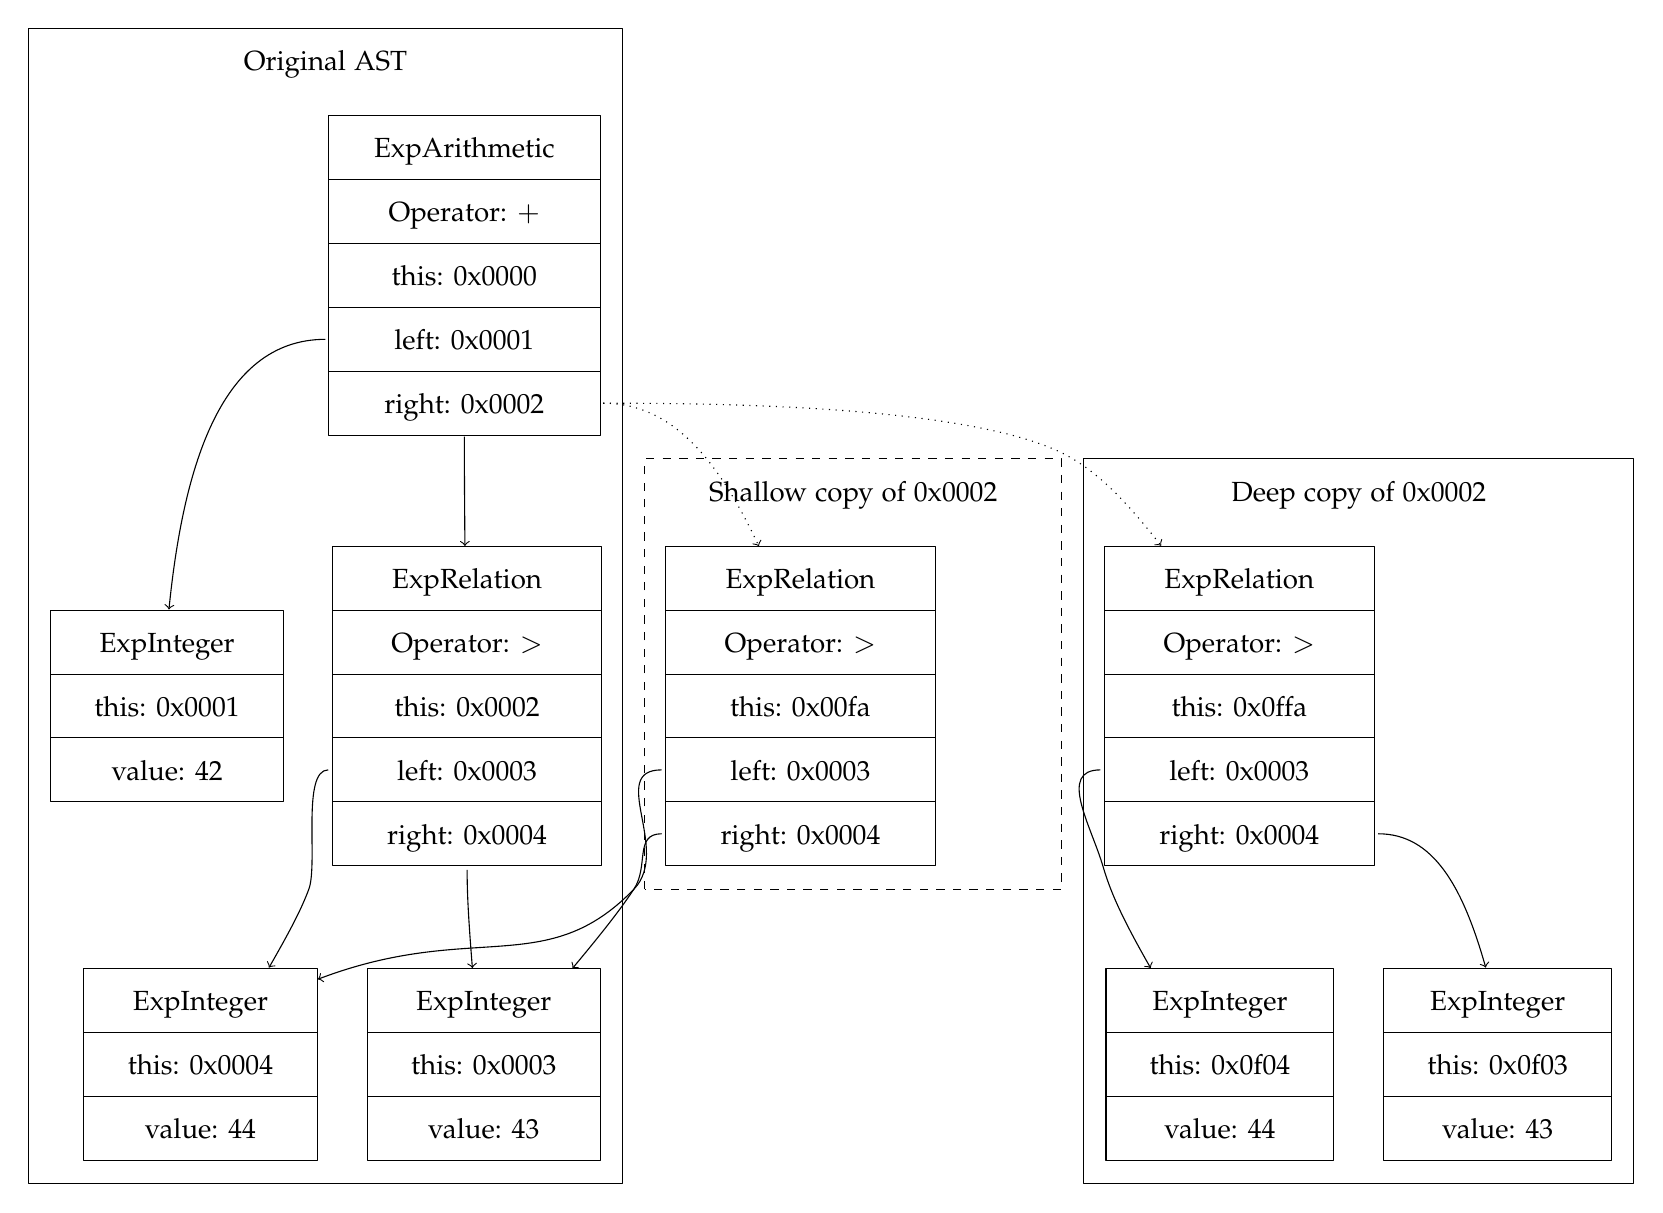
\begin{tikzpicture}[line join=bevel,anchor=base]%
\begin{scope}
  \pgfsetstrokecolor{black}
  \definecolor{strokecol}{rgb}{0.0,0.0,0.0};
  \pgfsetstrokecolor{strokecol}
  \draw (8.0bp,8.0bp) -- (8.0bp,424.0bp) -- (222.0bp,424.0bp) -- (222.0bp,8.0bp) -- cycle;
  \draw (115.0bp,408.8bp) node {Original AST};
\end{scope}
\begin{scope}
  \pgfsetstrokecolor{black}
  \pgfsetdash{{3pt}{3pt}}{0pt}
  \definecolor{strokecol}{rgb}{0.0,0.0,0.0};
  \pgfsetstrokecolor{strokecol}
  \draw [dashed] (230.0bp,114.0bp) -- (230.0bp,269.0bp) -- (380.0bp,269.0bp) -- (380.0bp,114.0bp) -- cycle;
  \draw (305.0bp,253.8bp) node {Shallow copy of 0x0002};
\end{scope}
\begin{scope}
  \pgfsetstrokecolor{black}
  \definecolor{strokecol}{rgb}{0.0,0.0,0.0};
  \pgfsetstrokecolor{strokecol}
  \draw (388.0bp,8.0bp) -- (388.0bp,269.0bp) -- (586.0bp,269.0bp) -- (586.0bp,8.0bp) -- cycle;
  \draw (487.0bp,253.8bp) node {Deep copy of 0x0002};
\end{scope}
  \pgfsetcolor{black}
  % Edge: c_c1 -> right
  \draw [->] (236.0bp,134.0bp) .. controls (226.06bp,134.0bp) and (231.53bp,122.26bp)  .. (226.0bp,114.0bp) .. controls (221.32bp,107.01bp) and (215.93bp,99.952bp)  .. (203.9bp,85.513bp);
  % Edge: a -> c_c1
  \draw [->,dotted] (215.0bp,289.0bp) .. controls (239.45bp,289.0bp) and (255.96bp,269.43bp)  .. (271.03bp,237.53bp);
  % Edge: a -> c_c2
  \draw [->,dotted] (215.0bp,289.0bp) .. controls (252.82bp,289.0bp) and (351.66bp,288.61bp)  .. (384.0bp,269.0bp) .. controls (393.78bp,263.07bp) and (402.34bp,254.86bp)  .. (415.85bp,237.71bp);
  % Edge: c_c2 -> right_c1
  \draw [->] (494.0bp,134.0bp) .. controls (513.66bp,134.0bp) and (524.35bp,115.28bp)  .. (532.7bp,85.826bp);
  % Edge: c -> left
  \draw [->] (116.0bp,157.0bp) .. controls (106.32bp,157.0bp) and (112.42bp,123.06bp)  .. (109.0bp,114.0bp) .. controls (106.55bp,107.53bp) and (103.38bp,101.0bp)  .. (94.651bp,85.8bp);
  % Edge: c_c2 -> left_c1
  \draw [->] (394.0bp,157.0bp) .. controls (378.44bp,157.0bp) and (390.63bp,136.94bp)  .. (395.0bp,122.0bp) .. controls (397.75bp,112.61bp) and (402.06bp,103.2bp)  .. (412.1bp,85.612bp);
  % Edge: c -> right
  \draw [->] (166.0bp,121.0bp) .. controls (166.0bp,112.79bp) and (166.43bp,104.06bp)  .. (167.9bp,85.641bp);
  % Edge: a -> b
  \draw [->] (115.0bp,312.0bp) .. controls (76.232bp,312.0bp) and (63.556bp,263.16bp)  .. (58.652bp,214.74bp);
  % Edge: c_c1 -> left
  \draw [->] (236.0bp,157.0bp) .. controls (216.38bp,157.0bp) and (239.65bp,128.1bp)  .. (226.0bp,114.0bp) .. controls (194.44bp,81.405bp) and (168.35bp,102.89bp)  .. (112.26bp,81.636bp);
  % Edge: a -> c
  \draw [->] (165.0bp,277.0bp) .. controls (165.0bp,267.54bp) and (165.05bp,257.55bp)  .. (165.21bp,237.6bp);
  % Node: a
\begin{scope}
  \definecolor{strokecol}{rgb}{0.0,0.0,0.0};
  \pgfsetstrokecolor{strokecol}
  \draw (116.0bp,277.5bp) -- (116.0bp,392.5bp) -- (214.0bp,392.5bp) -- (214.0bp,277.5bp) -- cycle;
  \draw (116.0bp,369.5bp) -- (214.0bp,369.5bp);
  \draw (116.0bp,346.5bp) -- (214.0bp,346.5bp);
  \draw (116.0bp,323.5bp) -- (214.0bp,323.5bp);
  \draw (116.0bp,300.5bp) -- (214.0bp,300.5bp);
  \draw (165.0bp,377.3bp) node {ExpArithmetic};
  \draw (165.0bp,354.3bp) node {Operator: \(+\)};
  \draw (165.0bp,331.3bp) node {this: 0x0000};
  \draw (165.0bp,308.3bp) node {left: 0x0001};
  \draw (165.0bp,285.3bp) node {right: 0x0002};
\end{scope}
  % Node: c
\begin{scope}
  \definecolor{strokecol}{rgb}{0.0,0.0,0.0};
  \pgfsetstrokecolor{strokecol}
  \draw (117.5bp,122.5bp) -- (117.5bp,237.5bp) -- (214.5bp,237.5bp) -- (214.5bp,122.5bp) -- cycle;
  \draw (117.5bp,214.5bp) -- (214.5bp,214.5bp);
  \draw (117.5bp,191.5bp) -- (214.5bp,191.5bp);
  \draw (117.5bp,168.5bp) -- (214.5bp,168.5bp);
  \draw (117.5bp,145.5bp) -- (214.5bp,145.5bp);
  \draw (166.0bp,222.3bp) node {ExpRelation};
  \draw (166.0bp,199.3bp) node {Operator: \(>\)};
  \draw (166.0bp,176.3bp) node {this: 0x0002};
  \draw (166.0bp,153.3bp) node {left: 0x0003};
  \draw (166.0bp,130.3bp) node {right: 0x0004};
\end{scope}
  % Node: b
\begin{scope}
  \definecolor{strokecol}{rgb}{0.0,0.0,0.0};
  \pgfsetstrokecolor{strokecol}
  \draw (16.0bp,145.5bp) -- (16.0bp,214.5bp) -- (100.0bp,214.5bp) -- (100.0bp,145.5bp) -- cycle;
  \draw (16.0bp,191.5bp) -- (100.0bp,191.5bp);
  \draw (16.0bp,168.5bp) -- (100.0bp,168.5bp);
  \draw (58.0bp,199.3bp) node {ExpInteger};
  \draw (58.0bp,176.3bp) node {this: 0x0001};
  \draw (58.0bp,153.3bp) node {value: 42};
\end{scope}
  % Node: left_c1
\begin{scope}
  \definecolor{strokecol}{rgb}{0.0,0.0,0.0};
  \pgfsetstrokecolor{strokecol}
  \draw (396.0bp,16.5bp) -- (396.0bp,85.5bp) -- (478.0bp,85.5bp) -- (478.0bp,16.5bp) -- cycle;
  \draw (396.0bp,62.5bp) -- (478.0bp,62.5bp);
  \draw (396.0bp,39.5bp) -- (478.0bp,39.5bp);
  \draw (437.0bp,70.3bp) node {ExpInteger};
  \draw (437.0bp,47.3bp) node {this: 0x0f04};
  \draw (437.0bp,24.3bp) node {value: 44};
\end{scope}
  % Node: right
\begin{scope}
  \definecolor{strokecol}{rgb}{0.0,0.0,0.0};
  \pgfsetstrokecolor{strokecol}
  \draw (130.0bp,16.5bp) -- (130.0bp,85.5bp) -- (214.0bp,85.5bp) -- (214.0bp,16.5bp) -- cycle;
  \draw (130.0bp,62.5bp) -- (214.0bp,62.5bp);
  \draw (130.0bp,39.5bp) -- (214.0bp,39.5bp);
  \draw (172.0bp,70.3bp) node {ExpInteger};
  \draw (172.0bp,47.3bp) node {this: 0x0003};
  \draw (172.0bp,24.3bp) node {value: 43};
\end{scope}
  % Node: c_c2
\begin{scope}
  \definecolor{strokecol}{rgb}{0.0,0.0,0.0};
  \pgfsetstrokecolor{strokecol}
  \draw (395.5bp,122.5bp) -- (395.5bp,237.5bp) -- (492.5bp,237.5bp) -- (492.5bp,122.5bp) -- cycle;
  \draw (395.5bp,214.5bp) -- (492.5bp,214.5bp);
  \draw (395.5bp,191.5bp) -- (492.5bp,191.5bp);
  \draw (395.5bp,168.5bp) -- (492.5bp,168.5bp);
  \draw (395.5bp,145.5bp) -- (492.5bp,145.5bp);
  \draw (444.0bp,222.3bp) node {ExpRelation};
  \draw (444.0bp,199.3bp) node {Operator: \(>\)};
  \draw (444.0bp,176.3bp) node {this: 0x0ffa};
  \draw (444.0bp,153.3bp) node {left: 0x0003};
  \draw (444.0bp,130.3bp) node {right: 0x0004};
\end{scope}
  % Node: c_c1
\begin{scope}
  \definecolor{strokecol}{rgb}{0.0,0.0,0.0};
  \pgfsetstrokecolor{strokecol}
  \draw (237.5bp,122.5bp) -- (237.5bp,237.5bp) -- (334.5bp,237.5bp) -- (334.5bp,122.5bp) -- cycle;
  \draw (237.5bp,214.5bp) -- (334.5bp,214.5bp);
  \draw (237.5bp,191.5bp) -- (334.5bp,191.5bp);
  \draw (237.5bp,168.5bp) -- (334.5bp,168.5bp);
  \draw (237.5bp,145.5bp) -- (334.5bp,145.5bp);
  \draw (286.0bp,222.3bp) node {ExpRelation};
  \draw (286.0bp,199.3bp) node {Operator: \(>\)};
  \draw (286.0bp,176.3bp) node {this: 0x00fa};
  \draw (286.0bp,153.3bp) node {left: 0x0003};
  \draw (286.0bp,130.3bp) node {right: 0x0004};
\end{scope}
  % Node: right_c1
\begin{scope}
  \definecolor{strokecol}{rgb}{0.0,0.0,0.0};
  \pgfsetstrokecolor{strokecol}
  \draw (496.0bp,16.5bp) -- (496.0bp,85.5bp) -- (578.0bp,85.5bp) -- (578.0bp,16.5bp) -- cycle;
  \draw (496.0bp,62.5bp) -- (578.0bp,62.5bp);
  \draw (496.0bp,39.5bp) -- (578.0bp,39.5bp);
  \draw (537.0bp,70.3bp) node {ExpInteger};
  \draw (537.0bp,47.3bp) node {this: 0x0f03};
  \draw (537.0bp,24.3bp) node {value: 43};
\end{scope}
  % Node: left
\begin{scope}
  \definecolor{strokecol}{rgb}{0.0,0.0,0.0};
  \pgfsetstrokecolor{strokecol}
  \draw (28.0bp,16.5bp) -- (28.0bp,85.5bp) -- (112.0bp,85.5bp) -- (112.0bp,16.5bp) -- cycle;
  \draw (28.0bp,62.5bp) -- (112.0bp,62.5bp);
  \draw (28.0bp,39.5bp) -- (112.0bp,39.5bp);
  \draw (70.0bp,70.3bp) node {ExpInteger};
  \draw (70.0bp,47.3bp) node {this: 0x0004};
  \draw (70.0bp,24.3bp) node {value: 44};
\end{scope}
\end{tikzpicture}}%

    \label{fig:cloneIllustration}
\end{figure}

% TODO: 3) constant folding für simple expressions
\subsection{Generic traverser}
\subsubsection{Traversal and evaluation}
Due to the recursive nature of an AST, its traversal plays a key role
in every compiler development. Arithmetic
expressions, for instance, could be modeled by
\ref{lst:classHierArith} (see also section \ref{sec:DataModel}).
%
\begin{lstlisting}[style=c++,caption={class hierarchy for integer
      arithmetic expression},label={lst:classHierArith}]
struct Exp { virtual ~Exp() {} };
struct Value  : Exp {
    int value; Value (int v) : value(v) {}
};

struct Plus   : Exp {
    Exp* left; Exp* right;
    Plus  (Exp* l, Exp* r) : left(l), right(r) {}
};

struct Minus  : Exp {
    Exp* left; Exp* right;
    Minus (Exp* l, Exp* r) : left(l), right(r) {}
};

struct Times  : Exp {
    Exp* left; Exp* right;
    Times (Exp* l, Exp* r) : left(l), right(r) {}
};

struct Divide : Exp {
    Exp* left; Exp* right;
    Divide(Exp* l, Exp* r) : left(l), right(r) {}
};
\end{lstlisting}
%
\begin{lstlisting}[style=c++,caption={Instance of a syntax
      tree},label={lst:classHierArithInst}]
Times *exp = new Minus(
  new Plus(
    new Times(new Value(2), new Value(3)),
    new Times(new Value(4), new Value(5))),
  new Divide(new Value(12), new Value(3))
);
\end{lstlisting}
%
Using the classes from listing \ref{lst:classHierArith}, the
arithmetic Expression \(2 \cdot 3 + 4 \cdot 5 - (12 / 3)\) may be
represented by listing \ref{lst:classHierArithInst}, which is exactly
how the parser itself constructs a syntax tree during its reduction
phase!

There are two main approaches how arithmetic expressions like
\ref{lst:classHierArithInst} could be evaluated. Because of the
importance of these techniques, both will be elaborated in detail
further below. The two evaluation methods are:
%
\begin{enumerate}
    \item \label{enum:evalFirst} OOP-like evaluation using member function traversal
    \item \label{enum:evalSec} Functional-style evaluation using an external traverser
\end{enumerate}
%
Evaluation with \ref{enum:evalFirst} requires additional member
functions in each of the classes of \ref{lst:classHierArith} (see
snippet \ref{lst:classHierArithEval}).
%
\begin{lstlisting}[style=c++,caption={Eval functions for expression
      AST},label={lst:classHierArithEval}]
// additional function in struct Exp:
    virtual int evaluate() = 0;

/* Further function declarations in structs Plus, Minus
   Divide, Times and Value intentionally left out */
int Plus::evaluate()  { return left->evaluate()+right->evaluate(); }
int Minus::evaluate() { return left->evaluate()-right->evaluate(); }
int Times::evaluate() { return left->evaluate()*right->evaluate(); }
int Divide::evaluate(){ return left->evaluate()/right->evaluate(); }
int Value::evaluate() { return this->value;                        }
\end{lstlisting}
%
With the new \CPP{eval} member function, the evaluation of the
arithmetic expression from \ref{lst:classHierArithInst}
becomes as easy as \CPP{exp->evaluate()}!
However, this evaluation method comes with two major drawbacks. First
of all, the evaluate function must redundantly be declared and
implemented for each leaf class of the AST hierarchy. In addition, listing
\ref{lst:classHierArithEval} shows that also the implementation only
differs in the respective arithmetic operation (\(+,\ -,\ \cdot\)
and \(/\)). Secondly, due to
the first point, the technique doesn't scale well. In more complex
AST's with more complex evaluation semantics, the complete traversal
process -- which is specified by the evaluation functions -- is spread
over each implementation file of every participating AST
class. That in turn, makes changes difficult to manage and bugs hard
to find, which is why Yodl makes no use of this traversal scheme.

Note: The vhdlpp transpiler from the IcarusVerilog project uses
exactly the same
scheme in order to transpile the VHDL AST into an semantically
equivalent Verilog source code (cf. \cite{VHDLPPREPO} file
\texttt{expression_emit.cc}).

However, there is another way of doing traversals over syntax
trees. Method \ref{enum:evalSec} (see enumeration from above) is a
technique
frequently found in a functional programming context. It uses so
called evaluation/traverser functions in order to extract meaning
(aka. semantics) from a given syntax tree. In classical denotational
semantics
an evaluation function is simply a side effect free function that maps
an AST onto a
mathematical object that represents the value of the evaluated (or
executed) abstract syntax tree (cf. \cite{SCH97}, in particular
2.2.2). A main characteristic of these
functions is that they use \emph{pattern matching} (cf. \cite{SCH97}
figure 4.2 for mathematical pattern matching)
%TODO: Glossary
in order to determine the type of the current node. Based on this type
information, the traverser function determines the fitting traversal
for the current AST node. C++, unfortunately, does not natively support
pattern matching as a language primitive. However, there are at least
two popular libraries -- Mach7 and SimpleMatch -- that implement such
functionality (cf. \cite{MACH7}, \cite{SIMPLEMATCH}). Both make
heavy use of template meta programming and are thus not easy to
understand and explain. For this reason the inner workings won't be
elaborated here. Also, no introduction to pattern matching will be
provided here, because of its wide adoption in the field of computer
science. Nevertheless, materials on that concept can be found in
\cite{LYAH} (chapter 4.1, ``Pattern matching'').

For listing \ref{lst:classHierArith}, a traverser (and
evaluator) can be built using
pattern matching with Mach7 and looks like snippet \ref{lst:travWithMach7}.
%
\begin{lstlisting}[style=c++,caption={Traverser with Mach7 pattern
      matching},label={lst:travWithMach7}]
int eval(Exp *expression){
    using namespace mch;
    using namespace std;
    var<int> i;
    var<Exp *> l, r;
    Match(expression){
        Case(C<Value>(i)){ return i; }
        Case(C<Plus>(l,r)){ return eval(l) + eval(r); }
        Case(C<Minus>(l,r)){ return eval(l) - eval(r); }
        Case(C<Times>(l,r)){ return eval(l) * eval(r); }
        Case(C<Divide>(l,r)){ return eval(l) / eval(r); }
        Otherwise(){ std::cout << "error!" << endl; }
    } EndMatch;
}
\end{lstlisting}
%
A natural language description of the source line
\begin{lstlisting}[style=c++]
    Case(C<Plus>(l,r)){ return eval(l) + eval(r); }
\end{lstlisting}
reads as follows: ``If the variable \CPP{expression} has the dynamic type
\emph{Plus}, then variable l and r will be bound to
\CPP{dynamic_cast<Plus>} \CPP{(expression)->left}
and \CPP{dynamic_cast<Plus>(expression)->left} respectively. If the
variable does not possess the type Plus, the succeeding line will be executed''.

For reasons of clarity, the mandatory binding template specializations
have been omitted. Without these specializations The \CPP{C<>}
template can not figure out what values it can bind to the
appropriate instances of \CPP{var<Exp *>}. %TODO: Reference of Mach7 example

\subsubsection{Generic traverser}
Especially for AST transformations, it is necessary to find each
node for whom a certain predicate holds true. A common example is loop
unrolling, which is described in \ref{sec:LoopExpansion}. Loop
expansion clearly makes only sense if it's applied on nodes of type
\CPP{ForLoopStatement}. For a compiler writer, the need following
algorithm \ref{alg:genericTraverser} arises.
%
\begin{algorithm}
    \caption{Abstract description of a generic traverser's behaviour}
    \begin{algorithmic}[0]
        \State \(rootNode \gets parseVHDL().getRoot()\)
        \State \(predicate \gets (\lambda type . \lambda node . node : type\))
        \\
        \Function{traverse}{node: AstNode *, predicate : (x -> bool), functor : (AstNode *
          -> void)}
        \If {\(predicate(node) = true\)}
        \State \(functor(node)\)
        \EndIf

        \For {\(\forall i \in node.childs\)}
        \If {\(predicate(i) = true\)}
        \State \(functor(i)\)
        \EndIf
        \State \Call{traverse}{i, predicate, functor}
        \EndFor
        \EndFunction
    \end{algorithmic}
    \label{alg:genericTraverser}
\end{algorithm}
%
\(Predicate\) is a higher-order function that takes one type and maps
it onto a new function that checks whether it's input matches this
type. A predicate could be constructed, for instance, using the expression
\[
    predicate\ ForLoopStatement = \lambda node . node : ForLoopStatements
\]
where ``:'' means ``has type of''. For a given node \(node\)
this anonymous function simply checks if \(node\) has the runtime type
of class \CPP{ForLoopStatement}.

The semantics of the traverse function from above shall be given in
natural language too: ``For any input node \(n\), the function \emph{traverse}
first tests if the predicate holds for \(n\). If it does, the function
\(functor\), given as parameter to \emph{traverse}, gets
executed. This function usually transforms the node in some
way. After that, \emph{traverse} iterates over all child nodes \(i\)
of node \(n\) and repeats the previous procedure for each \(i\).''

The class \CPP{GenericTraverser} implements this algorithm for the
complete class hierarchy depicted in \ref{fig:classHier} and can be
found in \texttt{generic_traverser.h}.
%
\begin{lstlisting}[style=c++,caption={Interface definition of the
      GenericTraverser class},label={lst:genericTraverserDecl}]
class GenericTraverser {
public:
    enum recur_t { RECUR, NONRECUR };
    GenericTraverser(
        std::function<bool (const AstNode*)> p,
        std::function<int (AstNode *,
                const std::vector<AstNode *> &)> v,
                recur_t r)
        /* Initializer List : */
        : isMutating(true) , isNary(true)
        , predicate(p) , mutatingNaryVisitorU(v)
        , recurSpec(r)
        { }

        /* The rest of the class internals
           intentionally omitted. */
};
\end{lstlisting}
%
Listing \ref{lst:genericTraverserDecl} shows a simplified version of
GenericTraverser's class declaration. The first constructor parameter
\CPP{p} resembles a so called type predicate, \CPP{v} is the
\emph{visitor} function and finally \CPP{r} is used to specify
additional behaviour of the traverser algorithm. The usage of an
generic traverser is shown by listing \ref{lst:genericTraverserUsage}.
%
\begin{lstlisting}[style=c++,caption={Example usage of an
      GenericTraverser object},label={lst:genericTraverserUsage}]
AstNode *ast = /* parsing intentionally omitted */;

StatefulLambda<int> cnt(
    0, [](const AstNode *, int &env) -> int { env++; return 0; });

GenericTraverser counter(
    makeNaryTypePredicate<ProcessStatement, WaitStmt>(),
    [&cnt](const AstNode *n) -> int { return cnt(n); },
    GenericTraverser::RECUR);

counter(ast);
std::cout << "Number of process and wait statements:"
          << counter.environment << std::endl;
\end{lstlisting}
%
Listing \ref{lst:genericTraverserUsage} uses a generic traverser
in order to count all AST nodes with a dynamic type of either
\CPP{ProcessStatement} or \CPP{WaitStmt}. It uses two currently
unknown infrastructure components:
%
\begin{enumerate}
    \item A type predicate generator
    \item and a stateful lambda.
\end{enumerate}
%
Chapter \ref{sec:typePredicates} describes both, hence a comprehensively
explanation is not included in this section. Put simply, a stateful
lambda is a C++ object with an overloaded call operator that possesses
an internal state that the functor modifies.
In the context of \ref{lst:genericTraverserUsage}, if \CPP{cnt}'s call
operator gets executed, it increments its internal state which is
a single integer number. In comparison to algorithm \ref{alg:genericTraverser}
the stateful lambda \CPP{cnt} is equal to the parameter \emph{functor}
of the \emph{traverser} function.
%
\begin{figure}[tb]
    \centering
    \caption{Generic traverser runtime behaviour}
    \resizebox{\textwidth}{!}{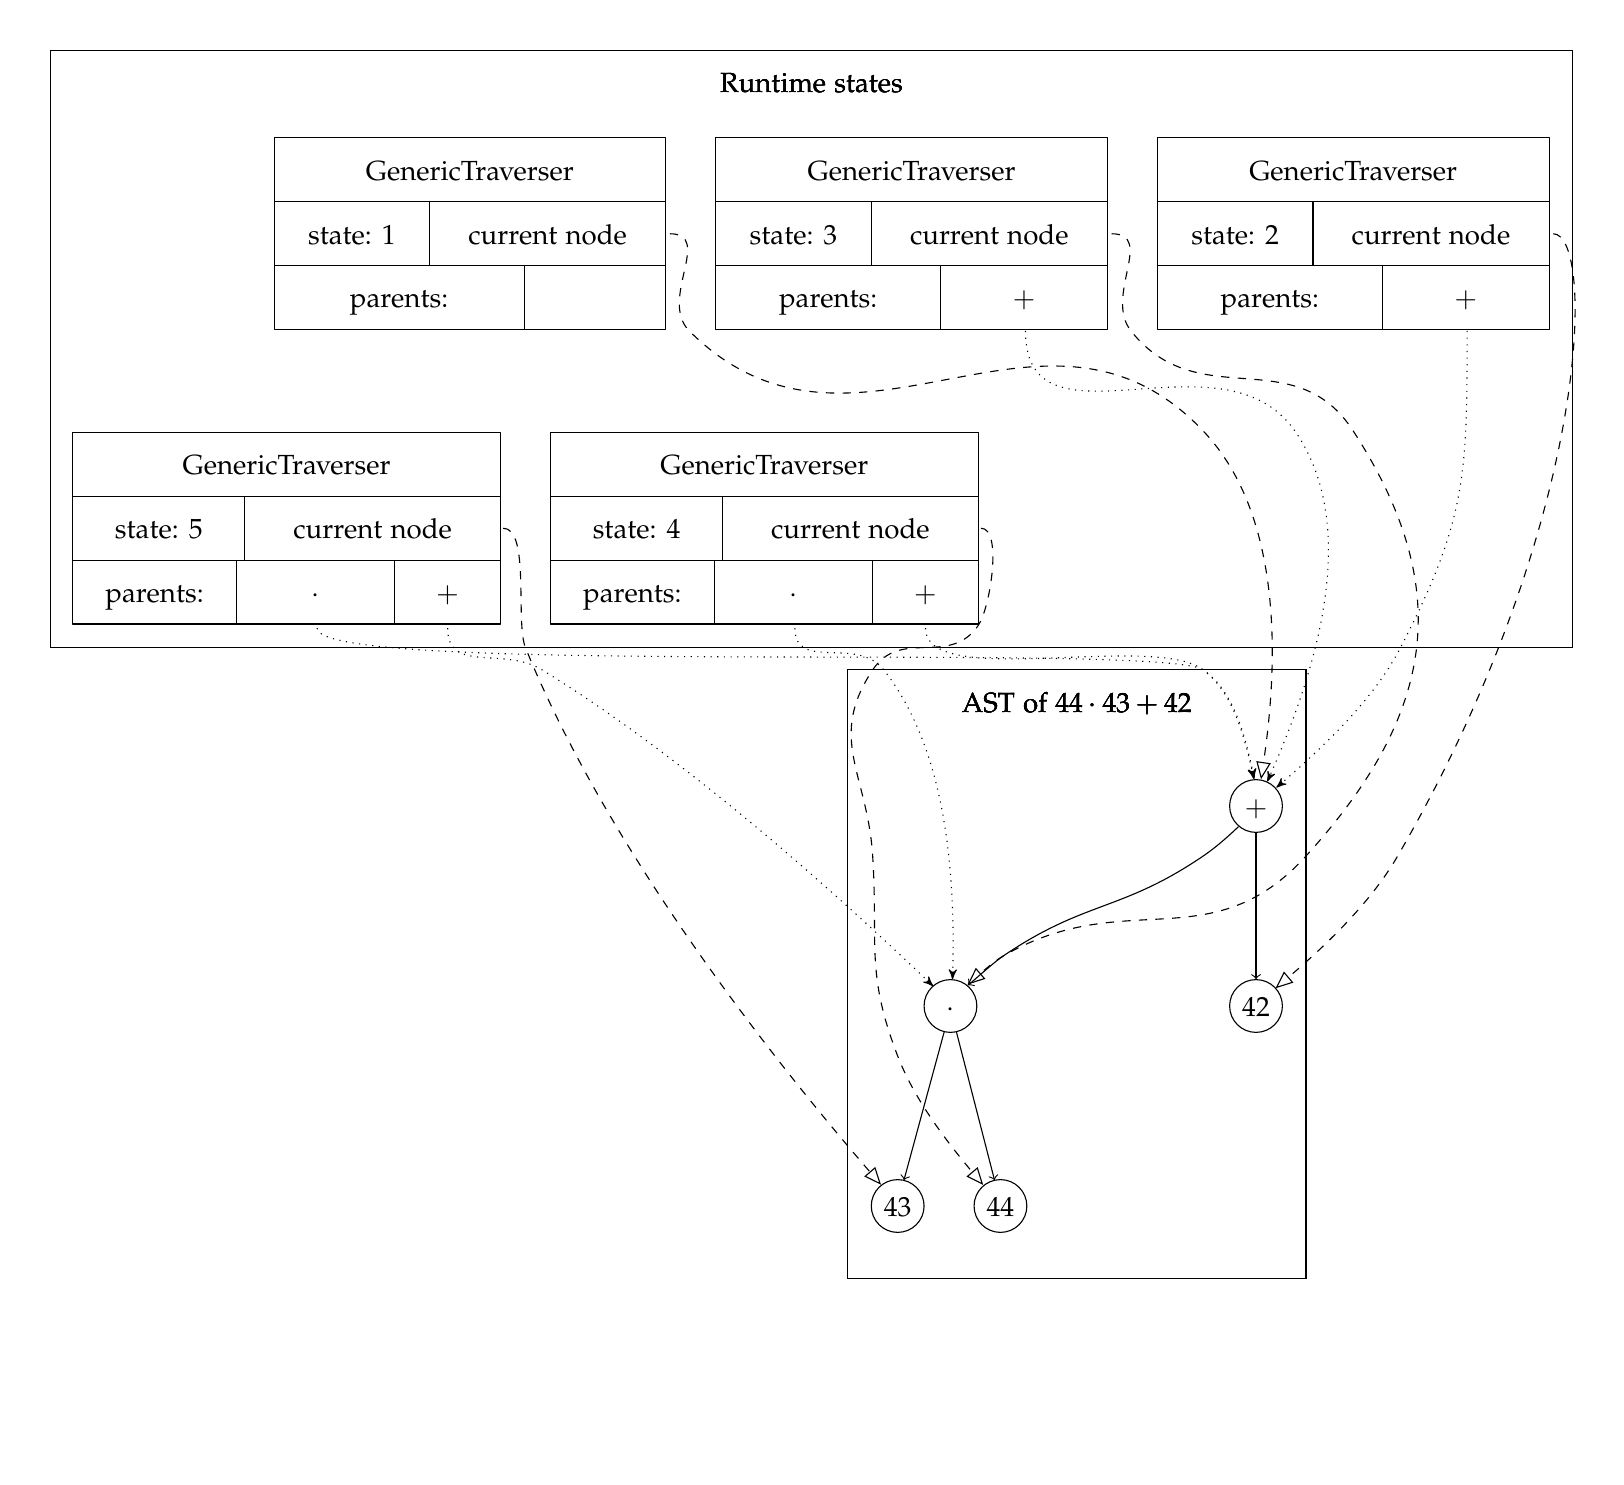
\begin{tikzpicture}[line join=bevel,anchor=base]%
\begin{scope}
  \pgfsetstrokecolor{black}
  \definecolor{strokecol}{rgb}{1.0,1.0,1.0};
  \pgfsetstrokecolor{strokecol}
  \definecolor{fillcol}{rgb}{1.0,1.0,1.0};
  \pgfsetfillcolor{fillcol}
  \filldraw (0.0bp,0.0bp) -- (0.0bp,514.0bp) -- (564.0bp,514.0bp) -- (564.0bp,0.0bp) -- cycle;
\end{scope}
\begin{scope}
  \pgfsetstrokecolor{black}
  \definecolor{strokecol}{rgb}{0.0,0.0,0.0};
  \pgfsetstrokecolor{strokecol}
  \draw (8.0bp,291.0bp) -- (8.0bp,506.0bp) -- (556.0bp,506.0bp) -- (556.0bp,291.0bp) -- cycle;
  \draw (282.0bp,490.8bp) node {Runtime states};
\end{scope}
\begin{scope}
  \pgfsetstrokecolor{black}
  \definecolor{strokecol}{rgb}{0.0,0.0,0.0};
  \pgfsetstrokecolor{strokecol}
  \draw (8.0bp,291.0bp) -- (8.0bp,506.0bp) -- (556.0bp,506.0bp) -- (556.0bp,291.0bp) -- cycle;
  \draw (282.0bp,490.8bp) node {Runtime states};
\end{scope}
\begin{scope}
  \pgfsetstrokecolor{black}
  \definecolor{strokecol}{rgb}{0.0,0.0,0.0};
  \pgfsetstrokecolor{strokecol}
  \draw (8.0bp,291.0bp) -- (8.0bp,506.0bp) -- (556.0bp,506.0bp) -- (556.0bp,291.0bp) -- cycle;
  \draw (282.0bp,490.8bp) node {Runtime states};
\end{scope}
\begin{scope}
  \pgfsetstrokecolor{black}
  \definecolor{strokecol}{rgb}{0.0,0.0,0.0};
  \pgfsetstrokecolor{strokecol}
  \draw (295.0bp,64.0bp) -- (295.0bp,283.0bp) -- (460.0bp,283.0bp) -- (460.0bp,64.0bp) -- cycle;
  \draw (377.5bp,267.8bp) node {AST of $44 \cdot 43 + 42$};
\end{scope}
\begin{scope}
  \pgfsetstrokecolor{black}
  \definecolor{strokecol}{rgb}{0.0,0.0,0.0};
  \pgfsetstrokecolor{strokecol}
  \draw (295.0bp,64.0bp) -- (295.0bp,283.0bp) -- (460.0bp,283.0bp) -- (460.0bp,64.0bp) -- cycle;
  \draw (377.5bp,267.8bp) node {AST of $44 \cdot 43 + 42$};
\end{scope}
\begin{scope}
  \pgfsetstrokecolor{black}
  \definecolor{strokecol}{rgb}{0.0,0.0,0.0};
  \pgfsetstrokecolor{strokecol}
  \draw (295.0bp,64.0bp) -- (295.0bp,283.0bp) -- (460.0bp,283.0bp) -- (460.0bp,64.0bp) -- cycle;
  \draw (377.5bp,267.8bp) node {AST of $44 \cdot 43 + 42$};
\end{scope}
\begin{scope}
  \pgfsetstrokecolor{black}
  \definecolor{strokecol}{rgb}{0.0,0.0,0.0};
  \pgfsetstrokecolor{strokecol}
  \draw (295.0bp,64.0bp) -- (295.0bp,283.0bp) -- (460.0bp,283.0bp) -- (460.0bp,64.0bp) -- cycle;
  \draw (377.5bp,267.8bp) node {AST of $44 \cdot 43 + 42$};
\end{scope}
  \pgfsetcolor{black}
  % Edge: c -> left
  \draw [->] (334.14bp,152.7bp) .. controls (336.87bp,142.06bp) and (341.68bp,123.35bp)  .. (347.87bp,99.294bp);
  % Edge: traverser_2 -> b
  \draw [-open triangle 45,dashed] (549.0bp,440.0bp) .. controls (564.03bp,440.0bp) and (563.47bp,337.75bp)  .. (493.0bp,216.0bp) .. controls (483.62bp,199.8bp) and (468.26bp,184.77bp)  .. (449.04bp,168.39bp);
  % Edge: traverser_5 -> c
  \draw [-stealth',dotted] (151.0bp,298.0bp) .. controls (151.0bp,281.48bp) and (170.92bp,291.63bp)  .. (185.0bp,283.0bp) .. controls (238.26bp,250.34bp) and (293.28bp,200.22bp)  .. (325.74bp,169.18bp);
  % Edge: traverser_5 -> right
  \draw [-open triangle 45,dashed] (171.0bp,334.0bp) .. controls (180.72bp,334.0bp) and (175.33bp,300.0bp)  .. (179.0bp,291.0bp) .. controls (210.16bp,214.56bp) and (273.0bp,137.03bp)  .. (307.0bp,97.663bp);
  % Edge: traverser_1 -> a
  \draw [-open triangle 45,dashed] (231.0bp,440.0bp) .. controls (246.86bp,440.0bp) and (226.75bp,416.19bp)  .. (238.0bp,405.0bp) .. controls (297.38bp,345.92bp) and (365.31bp,429.73bp)  .. (423.0bp,369.0bp) .. controls (452.72bp,337.72bp) and (449.58bp,282.37bp)  .. (443.8bp,243.63bp);
  % Edge: traverser_2 -> a
  \draw [-stealth',dotted] (518.0bp,405.0bp) .. controls (518.0bp,353.22bp) and (517.81bp,336.98bp)  .. (494.0bp,291.0bp) .. controls (484.96bp,273.56bp) and (468.99bp,257.56bp)  .. (449.36bp,240.65bp);
  % Edge: traverser_5 -> a
  \draw [-stealth',dotted] (104.0bp,298.0bp) .. controls (104.0bp,280.26bp) and (408.49bp,293.21bp)  .. (423.0bp,283.0bp) .. controls (432.46bp,276.34bp) and (437.22bp,264.18bp)  .. (441.33bp,243.86bp);
  % Edge: traverser_3 -> a
  \draw [-stealth',dotted] (359.0bp,405.0bp) .. controls (359.0bp,359.02bp) and (429.74bp,406.75bp)  .. (456.0bp,369.0bp) .. controls (480.64bp,333.57bp) and (462.49bp,279.6bp)  .. (446.07bp,242.83bp);
  % Edge: c -> right
  \draw [->] (329.75bp,152.7bp) .. controls (326.86bp,142.06bp) and (321.78bp,123.35bp)  .. (315.25bp,99.294bp);
  % Edge: traverser_4 -> a
  \draw [-stealth',dotted] (323.0bp,298.0bp) .. controls (323.0bp,275.53bp) and (405.14bp,296.64bp)  .. (423.0bp,283.0bp) .. controls (432.1bp,276.05bp) and (436.85bp,264.08bp)  .. (441.22bp,243.71bp);
  % Edge: traverser_4 -> left
  \draw [-open triangle 45,dashed] (343.0bp,334.0bp) .. controls (350.78bp,334.0bp) and (346.4bp,305.42bp)  .. (342.0bp,299.0bp) .. controls (331.65bp,283.88bp) and (314.14bp,298.27bp)  .. (304.0bp,283.0bp) .. controls (287.53bp,258.19bp) and (302.15bp,245.72bp)  .. (304.0bp,216.0bp) .. controls (306.0bp,183.81bp) and (301.43bp,174.1bp)  .. (313.0bp,144.0bp) .. controls (318.54bp,129.58bp) and (328.82bp,115.34bp)  .. (343.78bp,97.57bp);
  % Edge: a -> b
  \draw [->] (442.0bp,224.42bp) .. controls (442.0bp,213.92bp) and (442.0bp,195.85bp)  .. (442.0bp,171.65bp);
  % Edge: traverser_4 -> c
  \draw [-stealth',dotted] (276.0bp,298.0bp) .. controls (276.0bp,282.29bp) and (298.31bp,295.36bp)  .. (308.0bp,283.0bp) .. controls (331.19bp,253.42bp) and (333.79bp,207.42bp)  .. (332.74bp,171.62bp);
  % Edge: a -> c
  \draw [->] (435.68bp,226.56bp) .. controls (432.14bp,223.17bp) and (427.54bp,219.08bp)  .. (423.0bp,216.0bp) .. controls (393.41bp,195.89bp) and (380.59bp,200.11bp)  .. (351.0bp,180.0bp) .. controls (349.3bp,178.84bp) and (347.59bp,177.55bp)  .. (338.32bp,169.44bp);
  % Edge: traverser_3 -> c
  \draw [-open triangle 45,dashed] (390.0bp,440.0bp) .. controls (405.86bp,440.0bp) and (387.12bp,417.41bp)  .. (397.0bp,405.0bp) .. controls (421.29bp,374.5bp) and (455.83bp,401.74bp)  .. (477.0bp,369.0bp) .. controls (514.15bp,311.55bp) and (506.0bp,266.65bp)  .. (460.0bp,216.0bp) .. controls (425.7bp,178.23bp) and (395.16bp,205.55bp)  .. (351.0bp,180.0bp) .. controls (349.22bp,178.97bp) and (347.46bp,177.75bp)  .. (338.16bp,169.71bp);
  % Node: a
\begin{scope}
  \definecolor{strokecol}{rgb}{0.0,0.0,0.0};
  \pgfsetstrokecolor{strokecol}
  \draw (442.0bp,234.0bp) ellipse (9.5bp and 9.5bp);
  \draw (442.0bp,230.3bp) node {$+$};
\end{scope}
  % Node: c
\begin{scope}
  \definecolor{strokecol}{rgb}{0.0,0.0,0.0};
  \pgfsetstrokecolor{strokecol}
  \draw (332.0bp,162.0bp) ellipse (9.5bp and 9.5bp);
  \draw (332.0bp,158.3bp) node {$\cdot$};
\end{scope}
  % Node: b
\begin{scope}
  \definecolor{strokecol}{rgb}{0.0,0.0,0.0};
  \pgfsetstrokecolor{strokecol}
  \draw (442.0bp,162.0bp) ellipse (9.5bp and 9.5bp);
  \draw (442.0bp,158.3bp) node {$42$};
\end{scope}
  % Node: traverser_2
\begin{scope}
  \definecolor{strokecol}{rgb}{0.0,0.0,0.0};
  \pgfsetstrokecolor{strokecol}
  \draw (406.5bp,405.5bp) -- (406.5bp,474.5bp) -- (547.5bp,474.5bp) -- (547.5bp,405.5bp) -- cycle;
  \draw (406.5bp,451.5bp) -- (547.5bp,451.5bp);
  \draw (462.5bp,428.5bp) -- (462.5bp,451.5bp);
  \draw (406.5bp,428.5bp) -- (547.5bp,428.5bp);
  \draw (487.5bp,405.5bp) -- (487.5bp,428.5bp);
  \draw (477.0bp,459.3bp) node {GenericTraverser};
  \draw (434.5bp,436.3bp) node {state: 2};
  \draw (505.0bp,436.3bp) node {current node};
  \draw (447.0bp,413.3bp) node {parents:};
  \draw (517.5bp,413.3bp) node {$+$};
\end{scope}
  % Node: traverser_3
\begin{scope}
  \definecolor{strokecol}{rgb}{0.0,0.0,0.0};
  \pgfsetstrokecolor{strokecol}
  \draw (247.5bp,405.5bp) -- (247.5bp,474.5bp) -- (388.5bp,474.5bp) -- (388.5bp,405.5bp) -- cycle;
  \draw (247.5bp,451.5bp) -- (388.5bp,451.5bp);
  \draw (303.5bp,428.5bp) -- (303.5bp,451.5bp);
  \draw (247.5bp,428.5bp) -- (388.5bp,428.5bp);
  \draw (328.5bp,405.5bp) -- (328.5bp,428.5bp);
  \draw (318.0bp,459.3bp) node {GenericTraverser};
  \draw (275.5bp,436.3bp) node {state: 3};
  \draw (346.0bp,436.3bp) node {current node};
  \draw (288.0bp,413.3bp) node {parents:};
  \draw (358.5bp,413.3bp) node {$+$};
\end{scope}
  % Node: traverser_1
\begin{scope}
  \definecolor{strokecol}{rgb}{0.0,0.0,0.0};
  \pgfsetstrokecolor{strokecol}
  \draw (88.5bp,405.5bp) -- (88.5bp,474.5bp) -- (229.5bp,474.5bp) -- (229.5bp,405.5bp) -- cycle;
  \draw (88.5bp,451.5bp) -- (229.5bp,451.5bp);
  \draw (144.5bp,428.5bp) -- (144.5bp,451.5bp);
  \draw (88.5bp,428.5bp) -- (229.5bp,428.5bp);
  \draw (178.5bp,405.5bp) -- (178.5bp,428.5bp);
  \draw (159.0bp,459.3bp) node {GenericTraverser};
  \draw (116.5bp,436.3bp) node {state: 1};
  \draw (187.0bp,436.3bp) node {current node};
  \draw (133.5bp,413.3bp) node {parents:};
  \draw (204.0bp,413.3bp) node {};
\end{scope}
  % Node: traverser_4
\begin{scope}
  \definecolor{strokecol}{rgb}{0.0,0.0,0.0};
  \pgfsetstrokecolor{strokecol}
  \draw (188.0bp,299.5bp) -- (188.0bp,368.5bp) -- (342.0bp,368.5bp) -- (342.0bp,299.5bp) -- cycle;
  \draw (188.0bp,345.5bp) -- (342.0bp,345.5bp);
  \draw (250.0bp,322.5bp) -- (250.0bp,345.5bp);
  \draw (188.0bp,322.5bp) -- (342.0bp,322.5bp);
  \draw (247.0bp,299.5bp) -- (247.0bp,322.5bp);
  \draw (304.0bp,299.5bp) -- (304.0bp,322.5bp);
  \draw (265.0bp,353.3bp) node {GenericTraverser};
  \draw (219.0bp,330.3bp) node {state: 4};
  \draw (296.0bp,330.3bp) node {current node};
  \draw (217.5bp,307.3bp) node {parents:};
  \draw (275.5bp,307.3bp) node {$\cdot$};
  \draw (323.0bp,307.3bp) node {$+$};
\end{scope}
  % Node: traverser_5
\begin{scope}
  \definecolor{strokecol}{rgb}{0.0,0.0,0.0};
  \pgfsetstrokecolor{strokecol}
  \draw (16.0bp,299.5bp) -- (16.0bp,368.5bp) -- (170.0bp,368.5bp) -- (170.0bp,299.5bp) -- cycle;
  \draw (16.0bp,345.5bp) -- (170.0bp,345.5bp);
  \draw (78.0bp,322.5bp) -- (78.0bp,345.5bp);
  \draw (16.0bp,322.5bp) -- (170.0bp,322.5bp);
  \draw (75.0bp,299.5bp) -- (75.0bp,322.5bp);
  \draw (132.0bp,299.5bp) -- (132.0bp,322.5bp);
  \draw (93.0bp,353.3bp) node {GenericTraverser};
  \draw (47.0bp,330.3bp) node {state: 5};
  \draw (124.0bp,330.3bp) node {current node};
  \draw (45.5bp,307.3bp) node {parents:};
  \draw (103.5bp,307.3bp) node {$\cdot$};
  \draw (151.0bp,307.3bp) node {$+$};
\end{scope}
  % Node: right
\begin{scope}
  \definecolor{strokecol}{rgb}{0.0,0.0,0.0};
  \pgfsetstrokecolor{strokecol}
  \draw (313.0bp,90.0bp) ellipse (9.5bp and 9.5bp);
  \draw (313.0bp,86.3bp) node {$43$};
\end{scope}
  % Node: left
\begin{scope}
  \definecolor{strokecol}{rgb}{0.0,0.0,0.0};
  \pgfsetstrokecolor{strokecol}
  \draw (350.0bp,90.0bp) ellipse (9.5bp and 9.5bp);
  \draw (350.0bp,86.3bp) node {$44$};
\end{scope}
\end{tikzpicture}}%

    \label{fig:genTravRuntime}
\end{figure}
%
During the recursive, pre-order traversal, a generic traverser keeps
track of the current node and all of the nodes ancestors. Figure
\ref{fig:genTravRuntime} shows that if the traverser visits the leaf
node with value \(43\), the parent vector contains the node \(\cdot\)
as first and node \(+\) as second parent. If, at this state, the
requirements of the specified predicate would be met, the visitor
%
\begin{lstlisting}[style=c++]
std::function<int (AstNode *n,
        const std::vector<AstNode *> &)> v,
        recur_t r)
\end{lstlisting}
%
would be called with \(n = current\ node\) and \(v = [\cdot, +]\).

Internally a generic traverser object manages parent nodes with the
help of a stack. Each time it descents further down the abstract
syntax tree, it pushes the newly visited node onto the stack and
removes it again if the node itself or every child has been visited.

\subsection{Type predicates and stateful lambdas}
\label{sec:typePredicates}

This section presents two minor abstractions that have been proven to
be useful for Yodl's implementation. Stateful lambdas are located in
\texttt{stateful_lambda.h} and type predicates are defined in
\texttt{predicate_generators.h} and
\texttt{predicate_generators.cc}.

\subsubsection{Stateful lambdas}
\label{sec:statefulLambdas}
The generic traverser object uses the constructor shown in
\ref{lst:genericTraverserDecl} in order to specify visitor and
predicate functions for
traversal.
This constructor needs a C++ functional with the type
\begin{lstlisting}[style=c++]
std::function<bool (const AstNode*)> p
\end{lstlisting}

In principle, there are two ways to construct an object of that
type. On the one hand, C++-11's lambda syntax can be used as follows:
\begin{lstlisting}[style=c++]
[](AstNode *n) -> int { /* ... */ };
\end{lstlisting}
On the other hand, the usual and much more verbose way would be to
construct a normal C++ functor. In this context, a functor is an object
that overloads its call operator appropriately. Let the following
code be given as an example:
%
\begin{lstlisting}[style=c++]
class FunctorTemp {
    FunctorTemp() = default;

    int operator()(/* parameters */){ /* ... */ }
private:
    /* internal state variables here */
};
\end{lstlisting}
%
For functors without a persistent internal state, both sources are
exactly equivalent. However, lambdas created using the special notation
can not contain any private or
public member variables (aka. internal state), because there simply is
no special syntax for it. At first there seems to be no other way as to
stick to the lengthy functor class declaration, but stateful lambdas
provide a better solution for simple cases.

The class definition (\ref{lst:classStatefulLambda}) for
\CPP{StatefulLambda} illustrates how such an
improvement can be implemented.
Simply put, a \CPP{StatefulLambda} object encapsulates data together
with a C++ functor and provides a custom overload for the call
operator. That means it can be called like any other
function. However, instead of just executing the functor with the
parameter passed to \CPP{operator()}, it passes along a reference to
the internal state \CPP{environment} (see listing
\ref{lst:classStatefulLambda}).

Using this new abstraction a functor that counts nodes with particular
types can be build easily. Listing \ref{lst:genericTraverserUsage}
demonstrates a proper definition of a stateful lambda.

Note, because of clarity reasons, listing
\ref{lst:classStatefulLambda} does not contain all implementation
details.
%
\begin{lstlisting}[style=c++,caption={An interface for stateful
      lambdas},label={lst:classStatefulLambda}]
template<typename T> class StatefulLambda {
public:
    StatefulLambda(T e, std::function<int (AstNode *, T &)> l)
        : environment(e)
        , lambda(l) { }

    // environment gets default initialized in this constructor
    StatefulLambda(std::function<int (AstNode *, T &)> l)
        : lambda(l) { }

    int operator()(AstNode *node){
        return mutatingLambda(node, environment);
    }

    void reset(){
        environment = T();
    }

    T environment;
private:
    std::function<int (AstNode *, T &value)> lambda;
};
\end{lstlisting}
\subsubsection{Type predicates}
\label{sec:typePred}

In order to check whether a given visitor should be applied to a
current node during traversal, a generic traverser first executes a
previously specified predicate. As mentioned before, if this predicate
holds true, the visitor is executed, otherwise it is not.

While visitor functions can either have one or two parameters
every predicate must match the visitor signature established in
code \ref{lst:genericTraverserDecl}:
\begin{lstlisting}[style=c++]
std::function<bool (const AstNode*)>
\end{lstlisting}

Section \ref{sec:statefulLambdas} already showed the two main ways to
construct these callable objects. However, for type predicates,
template meta programming provides the means for an even shorter
function constructor. Listing \ref{lst:predicateGen} illustrates the
usage of a predicate constructor. It produces a predicate that maps a
pointer or a reference to an object to either true or false depending
on whether the dynamic type of the object occurs in the parameter list
of the \CPP{makeNaryTypePredicate} template.
%
\begin{lstlisting}[style=c++,caption={N-ary predicate
      generator},label={lst:predicateGen}]
makeNaryTypePredicate<ProcessStatement, IfSequential>();
\end{lstlisting}
%
Every C++11 compatible compiler can handle the meta function (listing
\ref{lst:predicateGen}) and
expands it in the fashion shown in listing \ref{lst:evalPredGen}. The
original unexpanded C++ meta code won't be printed here. However, this
source code can be examined in \texttt{predicate_generators.cc}.

Listing \ref{lst:evalPredGen} shows that the expansion results in an
cascaded if-else structure with appropriate Mach7 pattern matches. The
matches perform the necessary type checks and return either true if the
type matches the specified type or false if this isn't the case. The
complexity for the generated function is \(O(n)\), with \(n\) being
the number of template parameters of the \CPP{makeNaryTypePredicate}
template function. In the above case (listing \ref{lst:predicateGen}),
\(n = 2\), because only two type parameters -- \CPP{ProcessStatement}
and \CPP{IfSequential} -- have been used in order to instantiate the
function. The reason for the linear time complexity is the
progressively cascading if block illustrated by code
\ref{lst:evalPredGen}. Here, each additional type parameter used for
instantiation accounts for an additional nested type test block.
%
\begin{lstlisting}[style=c++,caption={Compile time evaluation of
      makeNaryTypePredicate},label={lst:evalPredGen}]
struct makeNaryTypePredicate {
  bool operator()(const AstNode *n){
    if (helper(n)) {
      return true;
    } else {
      /* anonymous class because of the template recursion */
      struct anon_inner {
        bool operator()(const AstNode *n){
          Match(n){
            CaseInT(mch::C<IfSequential>()){
              return true;
            }
          } EndMatch;
          return false;
        }
      };

      return anon_inner()(n);
    }
  }

  private:
  bool helper(const AstNode *n){
    Match(n){
      CaseInT(mch::C<ProcessStatement>()){
        return true;
      }
    } EndMatch;
    return false;
  }
};
\end{lstlisting}
\subsection{Localizing parser data structures}

Yodl uses vhdlpp's AST data model as well as its parser
implementation. Vhdlpp uses many global variables and data
structures for parsing VHDL (cf. \cite{VHDLPPREPO} revision 5dd2e6a, file
\texttt{entity.cc line 27}, \texttt{std_types.cc line 24, 26},
\ldots). In vhdlpp itself, this
does not pose a problem, because the whole program was built with the
intention to parse any given source file only once. As a consequence,
vhdlpp only produces one AST for each run and exits after it finished its
work. Yodl, however, uses smoke tests for verification
purposes. Thus, the need for disposable abstract syntax trees
arises. Of course, each of these trees could be build by hand, but
especially for larger structures this is a tedious and error prone
task. For that reason, a new class \CPP{ParserContext} has been
introduced and incorporates each of the previous global
structures. By means of this new data structure, unit tests can build
their own throw-away parser for the use of test AST construction.

The file \texttt{parse_context.h} serves as reference for this
refactoring effort.

\subsection{Testing}
\label{sec:autoTests}
Compilers are incredibly complex and complicated pieces of
software and thus notoriously difficult to test. There are a few
well known approaches for compiler validation. The first of which
is the so called regression test system\ldots

\subsubsection{Recression tests}
\label{sec:autoTestsReg}
The data base system \emph{SQLite}
for instance, uses such a validation framework (cf. \cite{SQLITE}).
In order to test sqlite's SQL interpreter, a TCL script
randomly generates SQL statements and evaluates them using the
interpreter and a predefined data base scheme. The script itself
manually calculates the result set and compares it with the output of
the SQL interpreter. If both result are exactly equal, the test
iteration was successful.

\emph{Vloghammer} uses a similar concept in order to validate Yosys'
Verilog
frontend. Akin to SQLite's regression tester, it randomly generates
syntactically and semantically correct Verilog code snippets,
synthesizes them with Yosys and checks the netlist
(cf. \cite{VLOGHAMMER}).

Such regression testing suites are incredibly useful, but also
difficult to implement. Hence, this work won't present an
implementation of this kind of automated test frameworks.

\subsubsection{Formal verification}
The second major compiler validation method uses formal tools. Such
validations are very hard to do, because every component of the
subjected translator must \emph{mathematically} be proven to work
according the the formal specification of the language. That's of
course only possible if there exists a formal description of the
language's semantics.

There indeed is such a specification, but only for an older version of
VHDL, which practically renders the formal verification method
unfeasible for VHDL-2008 (cf. \cite{VHDLFORM}).

\subsubsection{Smoke tests}

So called smoke tests, are much simpler to implement and --
if used correctly -- can limit the amount of bugs drastically. Tests
of this class are usually hand-coded by the compiler writer.

Yodl comes with a set of standard unit tests. At first, the header
only library \texttt{catch.h} has been used as unit testing
framework. Later, a switch to Cpputest was made (cf. \cite{CATCH},
\cite{CPPUTEST}). All tests are located in the files
\texttt{unit_tests_main.cc} and
\texttt{unit_tests_part1.cc}. Currently there are about \(1076\) lines
of test code.

\section{AST transformations}
\label{sec:astTrans}
All subsections in this chapter describe the various modifications
Yodl performs directly on the AST. Each transformation produces an
output AST as result. Although they don't directly generate netlists
or RTL descriptions, AST transformations like, for example, generate
expansion (in \ref{sec:GenerateExpansion}), must be performed in order
to simplify the AST. Even though netlists could be produced from a raw
unsimplified AST in theory, this would be, in practice, completely
unfeasible, because of the drastically higher code complexity.

\subsection{Loop expansion}
\label{sec:LoopExpansion}


All looping control structures must be statically unrolled. VHDL
describes hardware, that means there is no program counter that might
be utilized to implement sequential semantics. Furthermore, since VHDL
2008 (cf. \cite{IEEELRM})
does not impose any restrictions with regards to the nesting depth of
loops, unrolling is no trivial transformation. VHDL-2008 even allows
for the usage of \VH{next} and \VH{exit} statements inside of loop
bodies. This is a problem, because loops containing these control
statements are expected to behave like loops implemented in an
imperative and sequential programming language like C. But like
mentioned before, bare netlists don't contain primitive operations
like conditional branching (as provided by any assembly language).

VHDL's synthesis standard from 2004 (cf. \cite{IEEESYNTH})
explicitly forbids the use of \VH{while}-loops. However, in principle,
while loops containing arbitrary control expression, \emph{can} be
synthesized (cf. \cite{VHDLSYNTHESE}, in particular chapter
3.2.3.2). The high-level synthesis toolkit Legup
demonstrates this, because it allows for the synthesis from ANSI C
(including while loops) to behavioural-less\footnote{= Verilog without
 looping, always blocks, etc \ldots} Verilog. Legup accomplishes this by
creating finite state automata from the behavioural control structure
(cf. \cite{MSEM}, chapter 2.4.3).
The algorithms behind these transformations are very complicated and
not subject to further examination, at least in this
work. Nonetheless, \C{while} loops in C programs may contain the same two
troubling statements as VHDL models; \VH{next} \(\widehat{=}\) \C{continue}  and \VH{exit}
\(\widehat{=}\) \C{break}. That shows, that Legup's RTL synthesis algorithms are
at general enough to deal with loops containing an arbitrary number of
jumping statements.

\subsubsection{Prevention of complexity}
A very simple AST transformation method for general loop
unrolling is given in algorithm \ref{alg:loopPrePro}.

Here, the algorithm transforms every for loop containing an \VH{exit}
or \VH{next} statement into an equivalent while loop. As a
consequence, the \VH{for} loop unroller doesn't need to care about those
jump statements anymore, because after the illustrated AST
modification, there won't be any complicated for loops inside the
syntax tree anymore.

While this work presents an working for loop unroller, it does not
contain anything with regards to while loop synthesis. Like mentioned
above, VHDL 2004 does not allow for those loops to be written in
synthesizeable VHDL anyway.
%
\begin{algorithm}
    \caption{A generic loop pre-processing algorithm}
    \label{alg:loopPrePro}
    \begin{algorithmic}[0]
        \For{\(\forall i \in AST_{original}:
          isForloop(i) \land \neg containsForLoop(i)\)}
        \If{\(containsNext(i) \lor containsExit(i)\)}
        \State convertToWhile(i)
        \Else
        \State unroll(i)
        \EndIf
        \EndFor
    \end{algorithmic}
\end{algorithm}
%
\subsubsection{Special cases}

In certain cases, it is, however, possible to statically unroll a
given \VH{for} loop
even \emph{if} it contains \VH{next} or \VH{exit} clauses. First, the
appearance of next sequential statements shall be illuminated.
The first case, listing \ref{lst:firstCase}, is
probably the most obvious. Here, the next statement is executed inside
a simple if branch whose condition only depends on the loop index
variable -- that means that it is statically evaluable.
%
\begin{lstlisting}[style=vhdl,caption={First special
      case},label={lst:firstCase}]
for i in (0 to 2) loop
    if (i = 0) then
        next;
    end if;

    foo <= "001" + i;
end loop;

-- unrolls to
-------------
-- i = 0;
-- i = 1;
foo <= "001" + 1;
-- i = 2;
foo <= "001" + 2;
\end{lstlisting}
%
The second special case is almost as obvious as the first one, but
only of theoretical interest, because of its lack of usefulness. In
the case shown in \ref{lst:secondCase}, \VH{next} statements only occur at the first
level
below the for loop. As an example, consider the following snippet:
%
\begin{lstlisting}[style=vhdl,caption={Second special
      case},label={lst:secondCase}]
for i in (0 to 2) loop
    foo <= "001" + i;

    next;
    unreachedStmt1;
    unreachedStmt2;
    -- etc...
end loop;
\end{lstlisting}
%
Another interesting situation is depicted in the following listing
\ref{lst:thirdCase}.
Can this code be statically unrolled? That depends
on the properties that \VH{<expression>} possesses. First of all, it
has to be statically evaluable or else it's not possible to determine
the appropriate branch at compile time. Second of all, the if
condition must not
be modified by the statements \(ahead_1 \to ahead_n\). The reason
for the second constraint is given later. Under assumption of code
\ref{lst:thirdCase}, the source codes
\ref{lst:unrollingSchemeA} and \ref{lst:unrollingSchemeB} illustrate
the unrolling scheme.
%
\begin{lstlisting}[style=vhdl,caption={Third special case},label={lst:thirdCase}]
for i in (0 to 2) loop
    if (<expression>) then
        ahead_1;
        ahead_2;
        -- ...
        ahead_n;

        next;
    end if;

    <statement>;
end loop;
\end{lstlisting}


\noindent\begin{minipage}{0.45\textwidth}
\begin{lstlisting}[style=vhdl,caption={Unrolling
      Scheme -- First transformation},label={lst:unrollingSchemeA}]
for i in (0 to 2) loop
    if (<expression>) then
        ahead_1;
        ahead_2;
        -- ...
        ahead_n;
    end if;

    if (<expression>) then
        next;
    end if;

    <statements>;
end loop;























--
\end{lstlisting}
\end{minipage}\hfill
\begin{minipage}{0.45\textwidth}
\begin{lstlisting}[style=vhdl,caption={Unrolling
      Scheme -- Second transformation},label={lst:unrollingSchemeB}]
    --------
    -- i = 0
    if (<expression>) then
        ahead_1; ahead_2;
        -- ...
        ahead_n;
    end if;

    if (<expression>) then
        next;
    end if;

    <statements>;
    --------
    -- i = 1
    if (<expression>) then
        ahead_1; ahead_2;
        -- ...
        ahead_n;
    end if;

    if (<expression>) then
        next;
    end if;

    <statements>;
    -- i = 1
    if (<expression>) then
        ahead_1; ahead_2;
        -- ...
        ahead_n;
    end if;

    if (<expression>) then
        next;
    end if;

    <statements>;
\end{lstlisting}
\end{minipage}

\noindent{}For reasons regarding generality, the expansion step at the
end was not completely printed. Since it was stated that \VH{<expression>}
must be
statically evaluable, this evaluation needs to actually
happen. However, this is omitted here.

\subsection{Generate expansion}
\label{sec:GenerateExpansion}

VHDL contains two distinct syntactic domains where statements can
occur. The first one is the so called \emph{concurrent} and the
second one is the \emph{sequential} domain. Concurrent statements
can only occur in the statement part of an architecture body, whereas
sequential statements must be part of \VH{process} blocks. Note that
\VH{process} blocks itself are concurrent statements, at least from an
syntactic point of view (cf. \cite{IEEELRM}, Annex C -- Syntax summary).

So called generate statements belong to the syntactic class of
concurrent statements. These represent a kind of language
aware macro system, because with their help, code can be generated.
In this context, \emph{language aware} means that macros are expanded
on AST level rather than plain source code (text).

\subsubsection{How generate expansion works}
\begin{lstlisting}[style=vhdl,caption={A nested generate
      statement},label={lst:generateStmt}]
architecture behaviour of ForLoop is
   signal result : std_logic_vector(n downto 0);
begin
   gen : for i in 1 to 2 generate
      nested : for j in 1 to 1 + (i - 1) generate
         sum <= i + j + k;
      end generate nested;
   end generate gen;
end architecture;
\end{lstlisting}
%
Listing \ref{lst:generateStmt} gives a short example of a common
generate statement and the code from \ref{lst:generateStmtUnroll}
illustrates what those statements expand to.
%
\begin{lstlisting}[style=vhdl,caption={Generate statement unrolling},label={lst:generateStmtUnroll}]
architecture behaviour of ForLoop is
   signal result : std_logic_vector(n downto 0);
begin
   gen : block is
      constant i : natural := 1;
   begin
      nested : block is
         constant j : natural := 1;
      begin
         sum <= i + j + k;
      end block;
   end block gen;

   gen : begin block is
      constant i : natural := 2;
   begin
      nested : block is
         constant j : natural := 1;
      begin
         sum <= i + j + k;
      end block nested;

      nested : block is
         constant j : natural := 2;
      begin
         sum <= i + j + k;
      end block nested;
   end begin;
end architecture;
\end{lstlisting}
%
The above example shows, that more than one \VH{block} is labeled with
the same identifier. This is no error! VHDL-2008 explicitly requests
this kind of behavior during generate elaboration (cf. \cite{IEEELRM},
chapter 14.5.3 -- Generate statements).
Unelaborated generate statements can
themselves contain arbitrary declarations. These declarations will be
put into the respective declaration part of the expanded \VH{block}.
Note, that only \VH{block} or \VH{process} statements are able to create
new scopes inside of architecture statement parts.

\subsubsection{Presentation of an own generate expansion algorithm}

%TODO: rutscht zu weit weg aktuell. LAYOUT!
\begin{algorithm}
    \caption{Generate expansion algorithm}
    \label{alg:genExpansion}
    \begin{algorithmic}[1]
        \State \(rootNode \gets parseVHDL().getRoot()\)
        \State \(currentScope \gets nil\)
        \State \(currentEntity \gets nil\)
        \State \(statementAccumulator \gets nil\)
        \\
        \Function{modify}{statements : \&list<Statement*>}
        \State \(tmpStmts \gets nil\)
        \While {\(containsGenerateStmt(statements)\)}
        \For {\(\forall i \in statements\)}
        \If {\(i = NULL\)}
        \State \Return NotOK
        \EndIf

        \If {\(isGenerateStatement(i)\)}
        \State \Call{expandGenerate}{i}
        \State \(tmpStmts \gets statementAccumulator\)
        \State \(statementAccumulator \gets nil\)
        \Else
        \State \(tmpStmt \gets i\)
        \EndIf
        \EndFor

        \State \(statements \gets tmpStmts\)
        \State \(tmpStmts \gets nil\)
        \EndWhile

        \State \Return OK
        \EndFunction
        \\
        \Function{traverser}{n}
        \If {\(n : ScopeBase\)}
        \State \(currentScope \gets n\)
        \If {\(n : Architecture\)}
        \State \Return \Call{modify}{dynamic_cast<Architecture*>(n)->statements}
        \EndIf
        \If {\(n : BlockStatement\)}
        \State \Return \Call{modify}{dynamic_cast<BlockStatement*>(n)->concurrent_stmts_}
        \EndIf
        \ElsIf {\(n : Entity\)}
        \State \(currentEntity \gets n\)
        \EndIf
        \\
        \For{\(\forall i \in n.childs(): pointerNotNull(i)\)}
        \State \Call{traverser}{i}
        \EndFor
        \State
        \State \Return OK
        \EndFunction
    \end{algorithmic}
\end{algorithm}

With the use of the \CPP{GenericTraverser} class, it's very easy to
implement this algorithm. A generic traverser is used to model the
function \emph{traverser} shown above (see algorithm
\ref{alg:genExpansion}, line 27). In order to realize the logic
described by \emph{modify} (algorithm \ref{alg:genExpansion}, line 6),
a custom
C++ functor is needed. Recall
that a functor is just a C++ object with functional semantics. That
means it has some internal state -- as every other object -- and
can be called like an ordinary function; which means, that the object's
call operator must be overloaded. \CPP{GenerateExpander} is a class
that meets these requirements. Since the expander's implementation very much
follows the illustrated algorithm, it shall not be elaborated here any
further. The curious reader might consult the files
\texttt{generate_expander.cc} and \texttt{generate_expander.h} for
further implementation details.

Note that algorithm \ref{alg:genExpansion} contains an undefined
function in line 14. This function tries to evaluate the expression of
the generate statement. This expression can either be an arbitrary
condition or a simple range. In both cases, however, the function must
be able to evaluate the expression statically. If that's not possible,
an error will be reported and no expansion takes place. For an \VH{if}
generate statement, \emph{EXPANDGENERATE} simply encapsulates the
statements below the generate statement in a newly created block, but
only if the generate condition holds true. If the function, on the
other hand,
encounters a \VH{for} generate statement, the statement list of the
generate block will be replicated for each item in the specified
expression. After that, every statement list is placed in accordingly
created \VH{block}s analogously to the \VH{if} generate expansion.

\subsection{Elsif elimination}
\label{sec:ElsifElimination}

RTLIL generation is difficult, because the problem -- the algorithm
that generates RTLIL -- can not easily be broken up into sub
problems. The method, of course, can be split into different functions
that do their respective part of traversing over the syntax tree, but
% SEMANTIC that?
those functions still have their logical place in just one
class. The
more complicated the input gets, the more
complicated the RTLIL generator itself will be.
Hence, it makes sense to keep the input AST as simple as
possible. \VH{Elsif} elimination is one way to accomplish this.

\subsubsection{Example elimination}
VHDL provides special syntactic sugar inside of branch statements.
The general syntax for \VH{if}-\VH{else} clauses is given below (cf. \cite{IEEELRM}):
%
\begin{grammar}
<if_statement> ::= <if_part> <elsif_part> <else_part> `;'

<if_part> ::= [ <label> `:' ] `if' <expression> `then' <sequence_of_statements>

<elsif_part> ::= { `elsif' <expression> `then' <sequence_of_statements> }

<else_part> ::= [ `else' <sequence_of_statements> ] `end' `if' [ <label> ]
\end{grammar}
%
This (simplified) grammar allows for the source code
\ref{lst:ifWithElseif}.
%
\begin{lstlisting}[style=vhdl,caption={Original if statement with
      elsif},label={lst:ifWithElseif}]
if (s = "00") then
   op <= "0";
elsif (s = "01") then
   op <= "1";
else
   of <= "0";
end if;
\end{lstlisting}
%
Every \VH{elsif} clause can be mechanically
desugared into a nested branch statement only consisting of a \VH{if}
and (an optional) \VH{else} clause. For the previous code example
\ref{lst:ifWithElseif},
the listing \ref{lst:ifDesugared} demonstrates the process.
%
\begin{lstlisting}[style=vhdl,caption={Desugared if
      statement},label={lst:ifDesugared}]
if (s = "00") then
   op <= "0";
else
   if (s = "01") then
      op <= "1";
   else
      op <= "0";
   end if;
end if;
\end{lstlisting}
%
\subsubsection{Elimination Algorithm}
\begin{algorithm}
    \caption{A simple \VH{elsif} elimination algorithm}
    \label{alg:elsifElimination}
    \begin{algorithmic}[1]
        \For {\(\forall n \in AST_{original}\)}
        \If {n : IfSequential}
        \State \Call{eliminateElsif}{n :! IfSequential * }
        \EndIf
        \EndFor
        \\
        \Function{eliminateElsif}{ifStmt : IfSequential*>}
        \State elsifCarry : list<SequentialStmt *> \(\gets\) ifStmt->elsePart
        \State tmpResult : IfSequential

        \For {\(\forall i \in reverse(ifStmt->elsifList)\)}
        \State tmpResult \(\gets\) new IfSequential(i->condition,
        i->ifPart, nil, elsifCarry)
        \State elsifCarry \(\gets\) makeList(tmpResult)
        \EndFor

        \State ifStmt.elsifPart \(\gets\) nil
        \State ifStmt.elsePart \(\gets\) elsifCarry
        \\
        \State \Return OK
        \EndFunction
    \end{algorithmic}
\end{algorithm}
\noindent{}The algorithm \ref{alg:elsifElimination} shows type checks using the
operator \(:\). On the right-hand side, the name of the type is given,
whereas the left-hand side consists of a variable
identifier. Similarly, the \(:!\) operator denotes a dynamic type
conversion, which is also known as dynamic cast in C++. In assignment
contexts, where the assignment operator \(\gets\) is used, the
operator \(:\) shows the declared type of the variable subjected to
the assignment.

The implementation of algorithm \ref{alg:elsifElimination} can be
found in \texttt{elsif_eliminator.cc} and
\texttt{elsif_eliminator.h}. It is very short and concise with only 38
lines of code.
%
\subsection{If statement elimination}
\label{sec:ifStatementElimination}

Every if-else clause can be algorithmically transformed into an
equivalent case-when clause.
This is useful for the same reason described in section
\ref{sec:ElsifElimination}.
The listing \ref{lst:ifDesugared} transforms very easily into listing
\ref{lst:caseWhen}.
%
\begin{lstlisting}[style=vhdl,caption={Generated case when
      statement},label={lst:caseWhen}]
case (s = "00") is
   when TRUE  => op <= "0";
   when FALSE =>
      case (s = "01") is
         when TRUE  => op <= "1";
         when FALSE => op <= "0";
      end case;
end case;
\end{lstlisting}
%
The transition from if-else into case-when clauses can only be
performed
\begin{itemize}
    \item if the original expression from the \VH{if} statement does not
    contain any clock edge specification (cf. \cite{IEEESYNTH}, 6.1.2)
    \item and if the statement lists for the if and  else code path
    both contain exhaustive signal assignments (i.e. every signal from
    both paths gets at least one assignment).
\end{itemize}
%
If the above requirements are met, the transformation produces a
semantically equivalent AST, because of the following reasons:
\begin{itemize}
    \item The conditions, inside of a \VH{case} head, can be
    any syntactically valid expressions, as long as its evaluation
    results in something of a scalar\footnote{actually only std_logic
      or std_ulogic are allowed} or 1-dimensional array type. If
    it evaluates to an array type, the elements of the array must all
    have a scalar type (cf. \cite{IEEELRM}, 10.9). Since an \VH{if}
    statement condition must evaluate to either true or false, the
    first requirement holds (cf. \cite{IEEELRM}, 10.8), because true
    maps onto \VH{'1'} and false to \VH{'0'}.
    \item The conditions inside of the case alternative delimiters
    (\VH{when <exp> =>}) must be
    either scalar or of one dimensional array type, where the base
    type of that array has to scalar (cf. \cite{IEEELRM} 10.9). Since
    \VH{TRUE} and \VH{FALSE} are
    enumeration literals, they are scalar.
    \item Neither \VH{if} nor \VH{case} statements impose any
    restrictions onto the enclosed sequential statements.
\end{itemize}
%
The first sentence of this section states that the main reason for
this transformation is to make the AST simple enough to enable a less
complex AST \(to\) RTLIL transformation algorithm. This is still
valid, because of the fact that such a algorithm, effectively eliminates
a whole class of statements without changing the semantics of the AST.
There, however, is another reason why this kind of transformation is
useful. The RTL intermediate language of Yosys supports n-ary case
statements natively. Hence, the AST \(to\) RTLIL translator only has
to map each \VH{case} branch onto the according branch structure
inside the RTLIL data structure. The current netlist translator,
developed in the scope of this work, however, only produces simple
cells and makes no use of RTLIL's higher abstractions.

The files \texttt{ifelse_case_converter.cc} and
\texttt{ifelse_case_converter.h} specify and implement the shown
conversion method from \ref{alg:elsifElimination}.

\subsection{Process lifting}
\label{sec:Process lifting}

In VHDL, there are six different kinds of signal assignment statements
which are allowed in a statement list of an architecture or a
process.
%
\begin{itemize}
    \item Concurrent signal assignment statements
    \begin{enumerate}
        \item Simple concurrent signal assignment
        \item Conditional concurrent signal assignment
        \item Selected concurrent signal assignment
    \end{enumerate}

    \item Sequential signal assignment statements
    \begin{enumerate}
        \item Simple sequential signal assignment
        \item Conditional sequential signal assignment
        \item Selected sequential signal assignment
    \end{enumerate}
\end{itemize}
%
It is possible -- and required by the standard (cf. \cite{IEEELRM},
11.4) --
to convert all concurrent signal assignment statements to semantically
equivalent sequential assignments. In the context of this work, this
procedure is called \emph{process lifting}, because of the fact that a
ordinary concurrent statement gets lifted into an sequential
context; which is, of course, only present inside an \VH{process} block.

First, let there be some examples for the three kinds of concurrent
assignments. The listings \ref{lst:exampleSCSA}, \ref{lst:exampleCCSA}
and \ref{lst:exampleECSA} also contain a syntactic overview.
%
\begin{lstlisting}[style=vhdl,caption={Simple concurrent signal
      assignment},label={lst:exampleSCSA}]
-- BNF grammar:
---------------
-- Simple_Concurrent_Signal_Assignment ::=
--     Target "<=" [ "guarded" ] [ Delay_Mechanism ] Waveform ";";
-- Waveform ::= Expression | "null" | ...;
-- Rule for Delay_Mechanism intentionally ommitted

sigVector <= "01001001";
\end{lstlisting}
%
\begin{lstlisting}[style=vhdl,caption={Conditional concurrent signal
      assignment}, label={lst:exampleCCSA}]
-- BNF grammar:
---------------
-- Concurrent_Conditional_Signal_Assignment ::=
--     Target "<=" [ "guarded" ] [ Delay_Mechanism ] Conditional_Waveforms ";";
-- Target ::= Name | Aggregate;
-- Conditional_Waveforms ::= Waveform "when" Condition
--                           { "else" Waveform "when" Condition } [ "else" Waveform; ]

sigVector <= "1111" when (input = '0')
                 else "1000" when (input = '1')
                 else "0000";
\end{lstlisting}
%
\begin{lstlisting}[style=vhdl,caption={Selected concurrent signal
      assignment}, label={lst:exampleECSA}]
-- BNF grammar:
---------------
-- Concurrent_Selected_Signal_Assignment ::=
--     "with" Expression "select" Target "<="
--     [ Delay_Mechanism ]  { Waveform "when" [Choice] "," } ";" ;

with tmpInteger select sigVector <=
    "0001" when 0 | 1 | 42,
    "0010" when others;

\end{lstlisting}
%
The general scheme for appropriate encapsulation is simple on first
sight, but as soon as more details show up, it gets a lot more
complicated. In order to enclose one of the shown statements in a
process block, one simply has to create such a block using a snippet
like \ref{lst:exampleProcEnc}.
%
\begin{lstlisting}[style=vhdl,caption={Process encapsulation},
    label={lst:exampleProcEnc}]
sampleProc : process(tmpInteger) is
begin
    with tmpInteger select sigVector <=
        "0001" when 0 | 1 | 42,
        "0010" when others;
end process sampleProc;
\end{lstlisting}
%
What needs to be put in the sensitivity list, though? \cite{IEEELRM},
chapter 10.2,
provides an algorithm that has to be used to fill the sensitivity
list. Note, that it makes no semantic difference whether this
list of signals is written right after the \VH{process} keyword
enclosed in parentheses, or only as the arguments of an additional
\VH{wait} statement at the end of the process's sequence of
statements (cf. \cite{IEEELRM}, 10.2).

Because of the huge complexity, this work only implements a simplified
version of the official algorithm which can be found inside the files
\texttt{signal_extractor.cc} and \texttt{signal_extractor.h}. The
actual process lifting methods are encapsulated in the class
\CPP{CsaLifter} which is located in \texttt{csa_lifter.cc} and
\texttt{csa_lifter.h} respectively. The exact implementation details
are of no relevance for this work and have only been presented for
completeness.

\section{RTLIL generation}
\label{sec:RTLILgeneration}

The RTLIL generation is a process that transforms a (simplified) VHDL
abstract syntax tree into an functionally equivalent netlist. Netlists
have briefly been described in chapter \ref{sec:VHDL}.

The first subsection below will introduce the RTLIL netlist format
used by
Yosys' synthesis backend, the second specifies a set of requirements
of the input syntax tree and the third describes the netlist generator
algorithm itself.

\subsection{Yosys's RTLIL data structures}
\label{sec:rtlilStruct}

The term RTLIL stands for \emph{Register Transfer Logic Intermediate
Language}. However, it is not solely a formal language for netlists,
but also a set of C++ classes specifying an internal representation
that is easily interfaceable from within C++ programs. Figure
\ref{fig:classDiagRtlil} shows the most
important classes, their members and their relationship with each
other.

Any given RTLIL data structure can be serialized to \emph{ilang}, which
is the textual form of RTLIL. Of course, any valid ilang file can
also be deserialized again and be stored as common C++ data.

The class \CPP{Design} represents the core of any netlist. A
\CPP{Design} object is roughly equivalent to a VHDL top-level entity,
because it subsumes all participating submodules and provides for the
according interconnections between them. Every design can contain
arbitrarily many modules, whose purpose it is to hold wires, cells,
memories and processes as well as to connect them together. Modules
represent connections via the \CPP{connections} member which is simply
a list of \CPP{SigSig} objects. SigSig objects are 2-tuples that
associate one signal with another. Signals are modelled via the
\CPP{SigSpec} class. It must be noted, that every \CPP{Wire} object
can be converted to a \CPP{SigSpec} object, but not vice versa.

The enumeration \CPP{State} models every possible value a connection
between two cells in the netlist might hold. The last value,
\CPP{marker} is only used internally by some optimization passes.

Right at the end of the member list of \CPP{Module} there are still
two entries. The first map associates identifiers with \CPP{Memory}
objects which are used to model block RAM resources and the second
contains \CPP{Process} objects. Verilog and VHDL both offer sequential
(behavioural) hardware description. In both languages behavioural
modelling is only possible inside of \V{always} or \VH{process} blocks
respectively. RTLIL's \CPP{Process} objects try to emulate a part of
those semantics.

Memory and process objects are not relevant, which is
the reason for the ellipses in figure \ref{fig:classDiagRtlil}.
%
\begin{figure}[tb]
    \centering
    \caption{Important classes and their relationship}
    \input{graphs/classDiagRtlil.dot.tex}
    \label{fig:classDiagRtlil}
\end{figure}
%
As figure \ref{fig:yosysArch} from section \ref{sec:Yosys} shows,
there exists a backend that converts netlists into equivalent dot
graphs. This is very important for debugging purposes. The picture
\ref{fig:rtlilShow} contains a graph describing the netlist for the
full adder mentioned in section listing \ref{fulladd}.
%
\begin{figure}[tb]
    \centering
    \caption{Netlist for listing \ref{fulladd} generated by Yosys}
    \resizebox{\textwidth}{!}{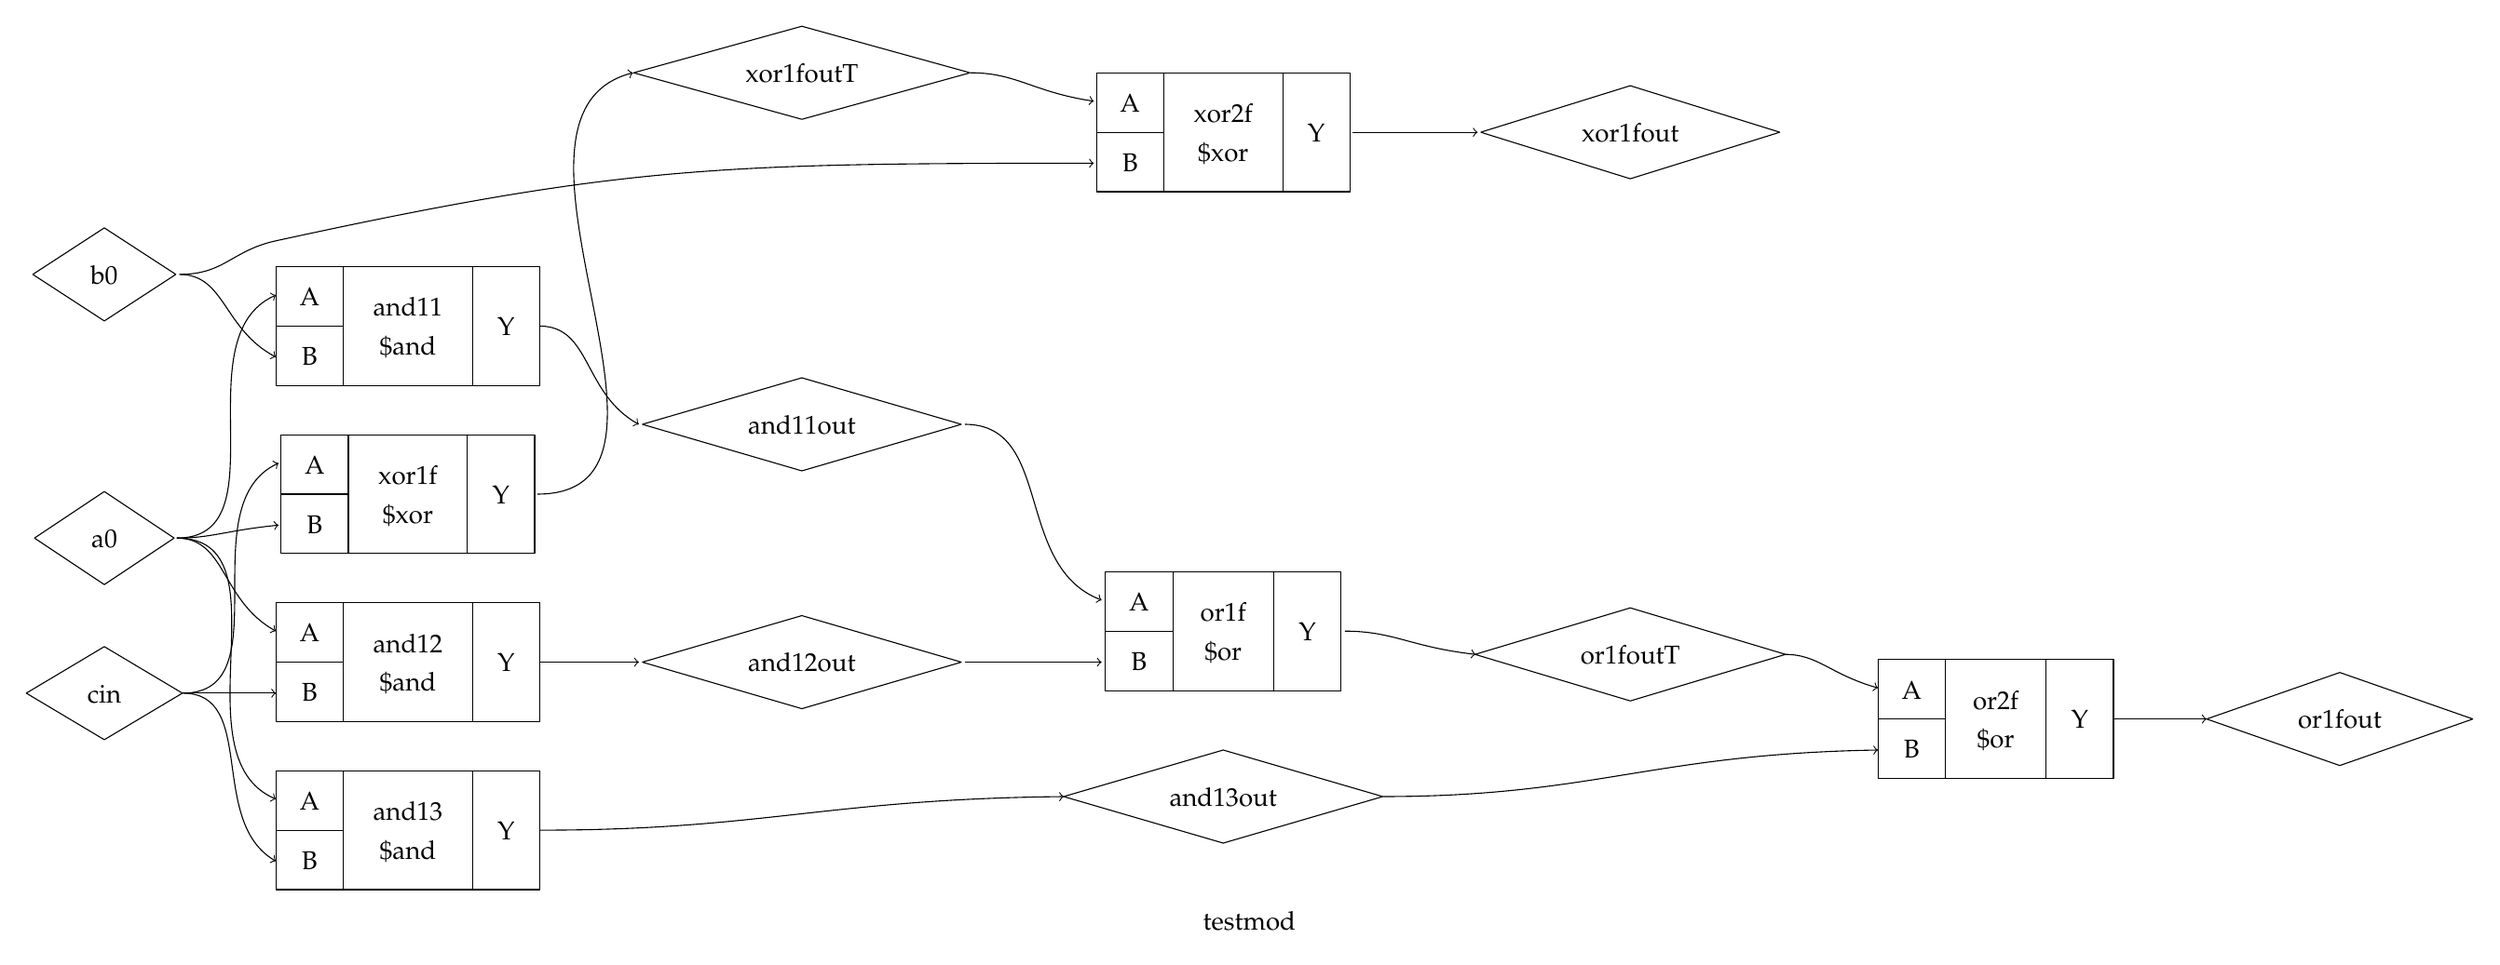
\begin{tikzpicture}[line join=bevel,anchor=base]%
\begin{scope}
  \definecolor{strokecol}{rgb}{0.0,0.0,0.0};
  \pgfsetstrokecolor{strokecol}
  \draw (472.89bp,7.8bp) node {testmod};
\end{scope}
  \pgfsetcolor{black}
  % Edge: n12 -> c23
  \draw [->] (679.84bp,114.5bp) .. controls (692.87bp,114.5bp) and (697.08bp,106.88bp)  .. (715.84bp,101.5bp);
  % Edge: c17 -> n7
  \draw [->] (197.66bp,176.5bp) .. controls (268.18bp,176.5bp) and (171.23bp,323.37bp)  .. (234.66bp,339.5bp);
  % Edge: c22 -> n12
  \draw [->] (509.77bp,123.5bp) .. controls (528.68bp,123.5bp) and (535.3bp,117.33bp)  .. (560.35bp,114.5bp);
  % Edge: n5 -> c19
  \draw [->] (59.332bp,261.5bp) .. controls (77.088bp,261.5bp) and (76.209bp,240.38bp)  .. (96.664bp,229.5bp);
  % Edge: c21 -> n11
  \draw [->] (198.66bp,46.5bp) .. controls (285.42bp,46.5bp) and (309.21bp,58.529bp)  .. (401.18bp,59.5bp);
  % Edge: n5 -> c18
  \draw [->] (59.332bp,261.5bp) .. controls (76.901bp,261.5bp) and (79.499bp,270.75bp)  .. (96.664bp,274.5bp) .. controls (231.18bp,303.85bp) and (269.77bp,304.49bp)  .. (412.77bp,304.5bp);
  % Edge: c18 -> n8
  \draw [->] (512.77bp,316.5bp) .. controls (530.39bp,316.5bp) and (537.17bp,316.5bp)  .. (561.1bp,316.5bp);
  % Edge: n7 -> c18
  \draw [->] (365.18bp,339.5bp) .. controls (382.99bp,339.5bp) and (389.0bp,332.1bp)  .. (412.77bp,328.5bp);
  % Edge: n3 -> c19
  \draw [->] (58.332bp,159.5bp) .. controls (99.397bp,159.5bp) and (60.09bp,237.37bp)  .. (96.664bp,253.5bp);
  % Edge: n11 -> c23
  \draw [->] (524.35bp,59.5bp) .. controls (606.33bp,59.5bp) and (628.57bp,76.054bp)  .. (715.84bp,77.5bp);
  % Edge: c19 -> n9
  \draw [->] (198.66bp,241.5bp) .. controls (218.51bp,241.5bp) and (215.29bp,215.44bp)  .. (236.92bp,203.5bp);
  % Edge: c23 -> n13
  \draw [->] (806.84bp,89.5bp) .. controls (818.84bp,89.5bp) and (824.09bp,89.5bp)  .. (842.84bp,89.5bp);
  % Edge: n10 -> c22
  \draw [->] (362.92bp,111.5bp) .. controls (382.56bp,111.5bp) and (389.88bp,111.5bp)  .. (415.77bp,111.5bp);
  % Edge: n9 -> c22
  \draw [->] (362.92bp,203.5bp) .. controls (397.31bp,203.5bp) and (381.67bp,148.61bp)  .. (415.77bp,135.5bp);
  % Edge: c20 -> n10
  \draw [->] (198.66bp,111.5bp) .. controls (211.68bp,111.5bp) and (217.23bp,111.5bp)  .. (236.92bp,111.5bp);
  % Edge: n1 -> c20
  \draw [->] (60.664bp,99.5bp) .. controls (72.664bp,99.5bp) and (77.914bp,99.5bp)  .. (96.664bp,99.5bp);
  % Edge: n3 -> c20
  \draw [->] (58.332bp,159.5bp) .. controls (77.504bp,159.5bp) and (75.289bp,135.28bp)  .. (96.664bp,123.5bp);
  % Edge: n1 -> c21
  \draw [->] (60.664bp,99.5bp) .. controls (89.56bp,99.5bp) and (70.167bp,49.734bp)  .. (96.664bp,34.5bp);
  % Edge: n3 -> c17
  \draw [->] (58.332bp,159.5bp) .. controls (71.961bp,159.5bp) and (77.495bp,162.49bp)  .. (97.664bp,164.5bp);
  % Edge: n3 -> c21
  \draw [->] (58.332bp,159.5bp) .. controls (102.22bp,159.5bp) and (57.787bp,75.113bp)  .. (96.664bp,58.5bp);
  % Edge: n1 -> c17
  \draw [->] (60.664bp,99.5bp) .. controls (99.486bp,99.5bp) and (63.149bp,172.59bp)  .. (97.664bp,188.5bp);
  % Node: c22
\begin{scope}
  \definecolor{strokecol}{rgb}{0.0,0.0,0.0};
  \pgfsetstrokecolor{strokecol}
  \draw (417.27bp,100.5bp) -- (417.27bp,146.5bp) -- (508.27bp,146.5bp) -- (508.27bp,100.5bp) -- cycle;
  \draw (417.27bp,123.5bp) -- (443.27bp,123.5bp);
  \draw (443.27bp,100.5bp) -- (443.27bp,146.5bp);
  \draw (482.27bp,100.5bp) -- (482.27bp,146.5bp);
  \draw (430.27bp,131.3bp) node {A};
  \draw (430.27bp,108.3bp) node {B};
  \draw (462.77bp,127.3bp) node {or1f};
  \draw (462.77bp,112.3bp) node {\$or};
  \draw (495.27bp,119.8bp) node {Y};
\end{scope}
  % Node: c23
\begin{scope}
  \definecolor{strokecol}{rgb}{0.0,0.0,0.0};
  \pgfsetstrokecolor{strokecol}
  \draw (715.84bp,66.5bp) -- (715.84bp,112.5bp) -- (806.84bp,112.5bp) -- (806.84bp,66.5bp) -- cycle;
  \draw (715.84bp,89.5bp) -- (741.84bp,89.5bp);
  \draw (741.84bp,66.5bp) -- (741.84bp,112.5bp);
  \draw (780.84bp,66.5bp) -- (780.84bp,112.5bp);
  \draw (728.84bp,97.3bp) node {A};
  \draw (728.84bp,74.3bp) node {B};
  \draw (761.34bp,93.3bp) node {or2f};
  \draw (761.34bp,78.3bp) node {\$or};
  \draw (793.84bp,85.8bp) node {Y};
\end{scope}
  % Node: c20
\begin{scope}
  \definecolor{strokecol}{rgb}{0.0,0.0,0.0};
  \pgfsetstrokecolor{strokecol}
  \draw (96.66bp,88.5bp) -- (96.66bp,134.5bp) -- (198.66bp,134.5bp) -- (198.66bp,88.5bp) -- cycle;
  \draw (96.66bp,111.5bp) -- (122.66bp,111.5bp);
  \draw (122.66bp,88.5bp) -- (122.66bp,134.5bp);
  \draw (172.66bp,88.5bp) -- (172.66bp,134.5bp);
  \draw (109.66bp,119.3bp) node {A};
  \draw (109.66bp,96.3bp) node {B};
  \draw (147.66bp,115.3bp) node {and12};
  \draw (147.66bp,100.3bp) node {\$and};
  \draw (185.66bp,107.8bp) node {Y};
\end{scope}
  % Node: c21
\begin{scope}
  \definecolor{strokecol}{rgb}{0.0,0.0,0.0};
  \pgfsetstrokecolor{strokecol}
  \draw (96.66bp,23.5bp) -- (96.66bp,69.5bp) -- (198.66bp,69.5bp) -- (198.66bp,23.5bp) -- cycle;
  \draw (96.66bp,46.5bp) -- (122.66bp,46.5bp);
  \draw (122.66bp,23.5bp) -- (122.66bp,69.5bp);
  \draw (172.66bp,23.5bp) -- (172.66bp,69.5bp);
  \draw (109.66bp,54.3bp) node {A};
  \draw (109.66bp,31.3bp) node {B};
  \draw (147.66bp,50.3bp) node {and13};
  \draw (147.66bp,35.3bp) node {\$and};
  \draw (185.66bp,42.8bp) node {Y};
\end{scope}
  % Node: n11
\begin{scope}
  \definecolor{strokecol}{rgb}{0.0,0.0,0.0};
  \pgfsetstrokecolor{strokecol}
  \draw (462.77bp,77.5bp) -- (401.1bp,59.5bp) -- (462.77bp,41.5bp) -- (524.44bp,59.5bp) -- cycle;
  \draw (462.77bp,55.8bp) node {and13out};
\end{scope}
  % Node: n13
\begin{scope}
  \definecolor{strokecol}{rgb}{0.0,0.0,0.0};
  \pgfsetstrokecolor{strokecol}
  \draw (894.32bp,107.5bp) -- (842.87bp,89.5bp) -- (894.32bp,71.5bp) -- (945.76bp,89.5bp) -- cycle;
  \draw (894.32bp,85.8bp) node {or1fout};
\end{scope}
  % Node: n12
\begin{scope}
  \definecolor{strokecol}{rgb}{0.0,0.0,0.0};
  \pgfsetstrokecolor{strokecol}
  \draw (620.1bp,132.5bp) -- (560.11bp,114.5bp) -- (620.1bp,96.5bp) -- (680.09bp,114.5bp) -- cycle;
  \draw (620.1bp,110.8bp) node {or1foutT};
\end{scope}
  % Node: n10
\begin{scope}
  \definecolor{strokecol}{rgb}{0.0,0.0,0.0};
  \pgfsetstrokecolor{strokecol}
  \draw (299.92bp,129.5bp) -- (238.26bp,111.5bp) -- (299.92bp,93.5bp) -- (361.59bp,111.5bp) -- cycle;
  \draw (299.92bp,107.8bp) node {and12out};
\end{scope}
  % Node: n8
\begin{scope}
  \definecolor{strokecol}{rgb}{0.0,0.0,0.0};
  \pgfsetstrokecolor{strokecol}
  \draw (620.1bp,334.5bp) -- (562.28bp,316.5bp) -- (620.1bp,298.5bp) -- (677.91bp,316.5bp) -- cycle;
  \draw (620.1bp,312.8bp) node {xor1fout};
\end{scope}
  % Node: n9
\begin{scope}
  \definecolor{strokecol}{rgb}{0.0,0.0,0.0};
  \pgfsetstrokecolor{strokecol}
  \draw (299.92bp,221.5bp) -- (238.26bp,203.5bp) -- (299.92bp,185.5bp) -- (361.59bp,203.5bp) -- cycle;
  \draw (299.92bp,199.8bp) node {and11out};
\end{scope}
  % Node: c19
\begin{scope}
  \definecolor{strokecol}{rgb}{0.0,0.0,0.0};
  \pgfsetstrokecolor{strokecol}
  \draw (96.66bp,218.5bp) -- (96.66bp,264.5bp) -- (198.66bp,264.5bp) -- (198.66bp,218.5bp) -- cycle;
  \draw (96.66bp,241.5bp) -- (122.66bp,241.5bp);
  \draw (122.66bp,218.5bp) -- (122.66bp,264.5bp);
  \draw (172.66bp,218.5bp) -- (172.66bp,264.5bp);
  \draw (109.66bp,249.3bp) node {A};
  \draw (109.66bp,226.3bp) node {B};
  \draw (147.66bp,245.3bp) node {and11};
  \draw (147.66bp,230.3bp) node {\$and};
  \draw (185.66bp,237.8bp) node {Y};
\end{scope}
  % Node: c18
\begin{scope}
  \definecolor{strokecol}{rgb}{0.0,0.0,0.0};
  \pgfsetstrokecolor{strokecol}
  \draw (413.77bp,293.5bp) -- (413.77bp,339.5bp) -- (511.77bp,339.5bp) -- (511.77bp,293.5bp) -- cycle;
  \draw (413.77bp,316.5bp) -- (439.77bp,316.5bp);
  \draw (439.77bp,293.5bp) -- (439.77bp,339.5bp);
  \draw (485.77bp,293.5bp) -- (485.77bp,339.5bp);
  \draw (426.77bp,324.3bp) node {A};
  \draw (426.77bp,301.3bp) node {B};
  \draw (462.77bp,320.3bp) node {xor2f};
  \draw (462.77bp,305.3bp) node {\$xor};
  \draw (498.77bp,312.8bp) node {Y};
\end{scope}
  % Node: n1
\begin{scope}
  \definecolor{strokecol}{rgb}{0.0,0.0,0.0};
  \pgfsetstrokecolor{strokecol}
  \draw (30.33bp,117.5bp) -- (0.17bp,99.5bp) -- (30.33bp,81.5bp) -- (60.5bp,99.5bp) -- cycle;
  \draw (30.33bp,95.8bp) node {cin};
\end{scope}
  % Node: n3
\begin{scope}
  \definecolor{strokecol}{rgb}{0.0,0.0,0.0};
  \pgfsetstrokecolor{strokecol}
  \draw (30.33bp,177.5bp) -- (3.33bp,159.5bp) -- (30.33bp,141.5bp) -- (57.33bp,159.5bp) -- cycle;
  \draw (30.33bp,155.8bp) node {a0};
\end{scope}
  % Node: c17
\begin{scope}
  \definecolor{strokecol}{rgb}{0.0,0.0,0.0};
  \pgfsetstrokecolor{strokecol}
  \draw (98.66bp,153.5bp) -- (98.66bp,199.5bp) -- (196.66bp,199.5bp) -- (196.66bp,153.5bp) -- cycle;
  \draw (98.66bp,176.5bp) -- (124.66bp,176.5bp);
  \draw (124.66bp,153.5bp) -- (124.66bp,199.5bp);
  \draw (170.66bp,153.5bp) -- (170.66bp,199.5bp);
  \draw (111.66bp,184.3bp) node {A};
  \draw (111.66bp,161.3bp) node {B};
  \draw (147.66bp,180.3bp) node {xor1f};
  \draw (147.66bp,165.3bp) node {\$xor};
  \draw (183.66bp,172.8bp) node {Y};
\end{scope}
  % Node: n5
\begin{scope}
  \definecolor{strokecol}{rgb}{0.0,0.0,0.0};
  \pgfsetstrokecolor{strokecol}
  \draw (30.33bp,279.5bp) -- (2.68bp,261.5bp) -- (30.33bp,243.5bp) -- (57.98bp,261.5bp) -- cycle;
  \draw (30.33bp,257.8bp) node {b0};
\end{scope}
  % Node: n7
\begin{scope}
  \definecolor{strokecol}{rgb}{0.0,0.0,0.0};
  \pgfsetstrokecolor{strokecol}
  \draw (299.92bp,357.5bp) -- (234.9bp,339.5bp) -- (299.92bp,321.5bp) -- (364.95bp,339.5bp) -- cycle;
  \draw (299.92bp,335.8bp) node {xor1foutT};
\end{scope}
\end{tikzpicture}}%

    \label{fig:rtlilShow}
\end{figure}
%
\subsection{Introduction of SVHDL}
\label{sec:svhdl}

The step from abstract syntax trees to netlists is complex enough by
itself. Because of that, it's only reasonable to keep the input AST as
simple as possible. An AST \(A\) is said to be simpler as \(B\) if
%
\begin{align*}
  & \mid t_A \mid < \mid t_B \mid,\ with \\
  & t_A = setOfTypes(A) \\
  & t_B = setOfTypes(B)
\end{align*}
%
The function \(setOfTypes\) maps each syntax tree onto a set of
all appearing types the nodes have. An intuitive example:
Let there be two different
production trees, one for \(1+2 \cdot 3\) (\(A\)) and one for \(1+2+2+2\)
(\(B\)). Now \(t_A = \{\mathbb{N}, +, \cdot\}\) and \(t_B =
\{\mathbb{N},+\}\) and furthermore \(\mid t_B \mid < \mid t_A \mid = 2
< 3\). Thus, \(B\) is simpler as \(A\).

Syntax trees are unseparable bound to their associated
context free grammars. The more different rules a grammar contains the
more different types the equivalent class hierarchy of the object
oriented AST incorporates\footnote{This fact won't be proven here}. As
a consequence a simpler AST can be specified not only by restrictions
on its actual data structure, but also by restrictions on the context free
grammar that generates this abstract tree.

The following BNF code presents the restrictions imposed on (parts of)
the original grammar resembling the so called simple VHDL (SVHDL).
%
\begin{grammar}
<sequential_statement> ::=
    <wait_statement> \alt
    <simple_signal_assignment_statement> \alt
    <simple_variable_assignment_statement> \alt
    <case_statement>

<concurrent_statement> ::=
    <block_statement> \alt
    <process_statement> \alt
    <component_instantiation_statement>
\end{grammar}
%
Originally, sequential statements could also be constructed from
following statements:
%
\begin{itemize}
    \item conditional_signal_assignment
    \item selected_signal_assignment
    \item conditional_variable_assignment
    \item selected_variable_assignment
    \item if_statement
    \item loop_statement
    \item next_statement
    \item exit_statement
    \item procedure_call_statement
    \item return_statement
\end{itemize}
%
Likewise, the concurrent statements rule hat following right-hand
sides:
%
\begin{itemize}
    \item concurrent_procedure_call_statement
    \item concurrent_assertion_statement
    \item concurrent_signal_assignment_statement
    \item generate_statement
\end{itemize}
%
Generate and for loop unrolling eliminates \emph{if_statement} and
\emph{generate_statement} as well as \emph{next_statement} and
\emph{exit_statement}. Procedure inlining is not part of this work,
but would remove \emph{return_statement} and
\emph{procedure_call_statement}. The standard for VHDL-2008 shows how
\emph{conditional_variable_assignment},
\emph{conditional_signal_assignment},
\emph{selected_variable_assignment} and
\emph{selected_signal_assignment} can be transformed in syntax trees
only consisting of \emph{if_statement},
\emph{simple_variable_assignment_statement},
\emph{simple_signal_assignment_statement} and
\emph{case_statement} (cf. \cite{IEEELRM}, 11.6). Chapter
\ref{sec:ifStatementElimination}
describes an algorithm with whom it is possible to eliminate
\emph{if_statement}. Finally,
\emph{concurrent_procedure_call_statement},
\emph{concurrent_assertion_statement} and
\emph{concurrent_signal_assignment_statement} can be wrapped in
\VH{process} statements and thus be transformed into
\emph{sequential_statement} and \emph{process_statement}.

The above elaboration only imposes syntactical restrictions onto
VHDL. In order to also specify semantical constraints, one has to use
precise mathematical tools, which would easily exceed the scope of
this thesis. Consequently, those restrictions will not be given here
neither formally nor informally.

\subsection{Synthesis semantics}

In standard \cite{IEEESYNTH}, a typical semantic specification begins
with a listing.
Given the snippet \ref{asyncReset}, the standard would describe what hardware
must synthesized. It does not specify what algorithm has to be used
for this task, as this is not the scope of such a specification.
%
\begin{lstlisting}[style=vhdl,caption={A typical IEEE 1076.6 code
      snippet},label={asyncReset}]
AsyncReset: process: (clock, reset)
begin
    if( reset = '1' ) then
        -- async assignment
        Q <= '0';
    elsif( rising_edge(clk) and reset = '0' ) then
        -- sync assignment
        Q <= D;
    end if;
end process;
\end{lstlisting}
%
The VHDL code in \ref{asyncReset} is expected to model a single clock
edge sensitive flip-flop with an asynchronous reset behavior.
The main characteristic of such a discrete component is fitting for
the code \ref{asyncReset}. If reset goes to value \(1\) the flip-flop
overwrites its current content with \(0\), otherwise the output \(Q\)
gets set only on occurrences of clock edges (cf. \cite{DIGITALTECHNIK},
11.4 -- D-Flipflops).

The remainder of this section is concerned with two things: The first
subsection will briefly and informally give a definition for the
semantics of certain structures and the second subsection will
show concrete synthesis results using Yodl.

\subsubsection{Semantics of simple assignments}

Given the assumption that an appropriate \VH{entity} declaration has
already been declared, the code
%
\begin{lstlisting}[style=vhdl]
simpleAssign: process(clock, reset)
begin
    foo <= "00011000";
end process;
\end{lstlisting}
%
shows a legal signal assignment statements. Note that the
enclosing \VH{architecture} has been omitted for reasons regarding
simplicity.

Let \VH{foo} have the array type \VH{std_logic_vector(downto)} with 8
members. Since the base type of such an array is equal to
\VH{std_logic}, the assignment of a string literal becomes
possible. In this case, the said string can only contain characters
representing the state that a single \VH{std_logic} value can have
(cf. \cite{IEEELRM}, 10.5).

The most important possible values of \VH{std_logic} are \VH{'0'},
\VH{'1'}, \VH{'z'} and \VH{'-'}, where \VH{'z'} describes a
high-impedance on the associated wire and \VH{'-'} simply means that
the value does not matter and can be anything. \VH{'-'} signals are
not relevant in this work (see figure \ref{fig:classDiagRtlil}).

Consequently, \VH{foo <= "00011000"} describes that the wires,
\VH{foo(7)} down to \VH{foo(0)}, shall be driven by the respective
signal values from the string literal. Hence, only \VH{foo(4)} and
\VH{foo(3)} are driven with the value \VH{'1'}.

\subsubsection{Semantics of variable assignments}

Since, VHDL was originally intended as a language for circuit
simulation rather than description, there are a few but important
differences between simulation semantics and synthesis
semantics. VHDL's reference manual, which describes mainly the
simulation semantics, states that all signal assignments encapsulated
inside an \VH{process} shall be accumulated until the very end of the
process' statement list. If this last statement has been executed,
only then every deferred signal assignment shall be executed at once.
Why this semantics was chosen, will not be elaborated any further
here. It should be clear, that only by using signal assignments
of processes, one can not easily model sequential behavior, because
of the previously described semantics. Hence, VHDL's designers
introduced the concept of \emph{variables}.

Unlike signal assignments, variable assignments show immediate
effect. In other words, if a variable gets updated inside a process
using an variable assignment statement, every subsequent usage of the
same variable identifier will refer to the right-hand side of the
latest assignment.

Listing \ref{lst:sigVar} shows how \VH{signals} and \VH{variables} have to
be declared and how values can be assigned to them.
%
\begin{lstlisting}[style=vhdl,caption={Declaration of variables and
      signals},label={lst:sigVar}]
fooP: process(clock, reset) is
    signal fooS : std_logic_vector(7 downto 0) := "00100111";
    variable fooV : std_logic_vector(7 downto 0) := "00100111";
begin
    -- assignment of a signal
    fooS <= "11111111";
    -- assignment of a variable
    fooV := "11111111";
end process;
\end{lstlisting}
%
Synthesis semantics and simulation semantics for variable assignments
are the same. However, this is not the case for signal
assignments. Due to the lack of time, variable assignments were not
implemented in the synthesis algorithm. Consequently, further
elaboration is not relevant here. There is, nevertheless, the
paragraph 3.3.1.4 in
book \cite{VHDLSYNTHESE} regarding variable assignment synthesis.

\subsubsection{Semantics of Case blocks}
\label{sec:semOfCase}

Case statements in VHDL are constructed as illustrated in code
\ref{lst:firstCaseStmt}.
The standard demands case expressions to be either of a scalar type
or of one-dimensional array type where the array type's base type must
be scalar. The \VH{when} clauses, following the \VH{case} keyword, must
be
exhaustive. In other words, for each possible value of the case
expression there must be one and only one matching choice. If not all
choices can reasonably be given -- for example if the width of the case
expression exceeds 5 bits -- a special VHDL keyword must be used:
\VH{others} (cf. \cite{IEEELRM}, 10.9).
%
\begin{lstlisting}[style=vhdl,caption={A typical IEEE 1076.6 code
      snippet},label={lst:firstCaseStmt}]
architecture b of e is
    signal fnord : std_logic_vector(1 downto 0);
    signal oddParity : std_logic;
begin
    AsyncReset: process(clock, reset, fnord)
    begin
        case fnord is
        -- fnord is called case expression
            when "00" => oddParity <= '1';
            -- when "00" is called a choice
            when "01" => oddParity <= '0';
            when "10" => oddParity <= '0';
            when "11" => oddParity <= '0';
        end case;
    end process;
end architecture b;
\end{lstlisting}
%
In VHDL all choices have to be matched in parallel
(cf. \cite{VHDLSYNTHESE}, 3.2.2). This behavior can
be achieved by synthesizing a \(n\)-muxer for each bit of each signal that
is assigned in all code paths below the initial case expression, where
\(n\) equals the number of bits of the case expression.

This transformation is very expensive as a case expression with just
8-bits leads to a synthesis of an 8-bit muxer for each assigned bit
wide signal. A \(n\)-bit muxer can be constructed using \(2^n-1\) 1-bit multiplexers.
An informal proof for this shall be given below:

Let \(mux\) be a function defined as
%
\begin{equation}
  \label{eq:muxer}
\text{mux}(\text{selector}, \text{sig}_0, \text{sig}_1) =
\begin{cases}
    \text{sig}_0 & \text{if } \text{selector} = 0 \\
    \text{sig}_1 & \text{if } \text{selector} = 1
\end{cases}
\end{equation}
%
The function \(mux\) can also be defined using boolean logic. Equation
\ref{eq:muxerBool} shows one possibility and table \ref{t:propcalc}
defines both functions in terms of a truth table.
%
\begin{equation}
    \label{eq:muxerBool}
    \text{mux}_{bool}(\text{selector}, \text{sig}_0, \text{sig}_1) =
    (\text{sig}_0 \land \overline{\text{selector}})
    \lor (\text{sig}_1 \land \text{selector}))
\end{equation}
%
\begin{table}[b]
\centering
\caption[Truthtable]{Truthtable for the equations
  \ref{eq:muxer} and \ref{eq:muxerBool}}
% generated by sagemath's latex function
%%
\begin{tabular}{llll}\(sig_0\) & \(selector\) & \(sig_1\) &
                                                            \(mux(selector,
                                                            sig_0, sig_1)\)\\\hline False & False & False & False \\False & False & True & False \\False & True & False & False \\False & True & True & True \\True & False & False & True \\True & False & True & True \\True & True & False & False \\True & True & True & True\end{tabular}

\label{t:propcalc}
\end{table}
%
Now, a n-ary muxer function can be defined recursively using equation
\ref{eq:muxerNary}.
A 3-muxer for example, must be able to cope with \(2^3\) different
input ports and can be created by using \(k = 2\). The
3-bit selector is thus sufficient to select any of the given
signals. Each recursion step, \((k-1)\), produces one muxer and binds the
outputs of further two multiplexers onto its input. For \(mux_k\)
there are \(k+1\) steps in the recursion. Each step adds twice as much
multiplexers to the circuit as the step before, accounting for an
overall count of \(2^{k+1}-1\) multiplexers for
\(mux_k\)\footnote{Figure \ref{fig:netlistCaseStmt} shows a netlist
  for a 3-bit multiplexer}.

\begin{equation}
    \label{eq:muxerNary}
    \begin{aligned}
        mux_0(a, b, c) &=  mux(a, b, c) \\
        mux_k(s_k, iZ_{2^k-1}, iZ_{2^k-2}, \ldots, iZ_{0}) &=
        mux(s_{k-1}, \\
        &\qquad mux_{k-1}(s_{k-1}, iZ_{2^k-1}, iZ_{2^k-2}, \ldots,
        iZ_{2^{k-1}}), \\
        &\qquad mux_{k-1}(s_{k-1}, iZ_{2^{k-1}-1}, \ldots, iZ_{0}))
  \end{aligned}
\end{equation}

\subsubsection{Semantics of if statements}

In normal programming languages, if statements are a way to model
branches in the execution path of the program. Depending on the
evaluation of a condition, either the \emph{true} path or the
\emph{false} path will be chosen. In VHDL's synthesis semantics,
however, if statements are used to describe memories.
Given the example code \ref{lst:condAssign},
%
\begin{lstlisting}[style=vhdl,caption={Simple conditional assignment},
   label={lst:condAssign}]
if (clock = '1' and clock'event) then
    A <= B;
end if;
\end{lstlisting}
%
\VH{A <= B} appears as though it's only executed if the condition is
true. This is simply not the case here. A connection between node
\VH{A} and \VH{B} in the netlist is made either way, but it's the type
of connection that matters. Instead of a simple wire going from \VH{B}
to \VH{A}, a memory element with a certain conditional \emph{runtime}
behavior has to be utilized in between in order to achieve the
modeled sequential behavior (cf. \cite{IEEESYNTH}, 6.1).

As the figure \ref{fig:netlistMotSync} shows very clearly, an edge
sensitive flip-flop is
the synthesis result of listing \ref{lst:motSync}'s synthesis. This is the
consequence of the controlling \VH{if} condition at the top of listing
\ref{lst:motSync}. The semantics here are that \VH{A} will only get
assigned the current value of \VH{B}, if and only if a rising edge on
\VH{clock} is detected.

Level sensitive storage elements like, for instance, D-Latches, can also
be synthesized. Consider for example the snippet \ref{lst:dLatch}.
%
\begin{lstlisting}[style=vhdl, caption={Simple D-Latch being
      utilized}, label={lst:dLatch}]
if (foo + 3 < bar - 15) then
    A <= B;
end if;
\end{lstlisting}
%
Neither \VH{foo} nor \VH{bar} are declared to be clock signals but are
just ordinary wires transmitting data. However, the assignment (in
hardware) shall only be apparent on \VH{A} if and only if the
condition evaluates to true. So how does one get this behaviour in a
unchangeable circuit. Like above, it comes down to discrete elements
that can remember data (cf. \cite{IEEESYNTH}, 6.2). In the synthesis
result of code \ref{lst:dLatch}, the assignment is not done through a
DFF. Instead a D-Latch sits between the signals \VH{A} and
\VH{B}. As clock input for the latch serves the netlist for the if
expression \VH{foo + 3 < bar - 15} (cf. section
\ref{sec:SimpleLatchedAssign}).

The only difference between listings \ref{lst:dLatch} and
\ref{lst:condAssign} is the missing clock edge specification in
listing \ref{lst:dLatch}. The following paragraph will inform about
the nature of clock edges and explains the term synchronous condition.

\paragraph{Clock edge specification}
According to \cite{IEEESYNTH} 6.1.2
there are 10 ways how a clock edge can be described in VHDL. These are
shown in code \ref{lst:clockEdge}.
%
\begin{lstlisting}[style=vhdl,caption={Clock edge specification syntax
    in VHDL},label={lst:clockEdge}]
-- rising clock edge modelling
clock = '1'      and clock'event
clock = '1'      and not clock'stable
clock'event      and clock = '1'
not clock'stable and clock = '1'
rising_edge(clock)

-- falling clock edge modelling
clock = '0'      and clock'event
clock = '0'      and not clock'stable
clock'event      and clock = '0'
not clock'stable and clock = '0'
falling_edge(clock)
\end{lstlisting}
%
\VH{falling_edge(clock)} and \VH{rising_edge(clock)}, in particular, are
more than just procedure calls abbreviating the above mentioned long
versions of clock edge specificators. This is a detail of VHDL and not
relevant here.

\paragraph{A Synchronous condition} is a condition (i.e. expression)
that contains a clock edge specification and is true only if the clock
edge specification evaluates true. This connection can be made formal
by the following boolean predicate \ref{eq:syncCond}.
%
\begin{equation}\label{eq:syncCond}
    \begin{aligned}
        \text{syncCond}(c) & = \text{typeOfBool}(c) \land \\
        &\qquad \text{containsClockEdge}(c) \\
        &\qquad (c = \text{true} \to \text{clockEdge}(c) = \text{true})
    \end{aligned}
\end{equation}
%
As an example consider the VHDL expression:
%
\begin{lstlisting}[style=vhdl]
en = '1' and (clock = '1' and clock'event)
\end{lstlisting}
%
Now, the according boolean formula for \(c\) can be extracted and used
in the previously defined predicate.
%
\begin{equation}
    \begin{aligned}
        \text{let } c :&= (\text{en} = \text{true} \land \text{clock})
        \implies \text{clockEdge}(c) = \text{clock} \\
        \text{syncCond}(c) &= \text{typeOfBool}(c) \\
        &\qquad \land \text{containsClockEdge}(c) \\
        &\qquad \land ((\text{en} = \text{true} \land \text{clock}) =
        \text{true} \to \text{clock} = 1)
    \end{aligned}
\end{equation}
%
Hence, a synchronized condition must be of type boolean, it must contain
at least one clock edge and finally, the expression
\[
    ((\text{en} = \text{true} \land \text{clock}) = \text{true} \to
    \text{clock} = 1)
\]
%
must evaluate true for each possible binding of \(en\) and
\(clock\). In this case there are exactly \(2^2\) possible bindings.

\subsection{Transformation algorithm -- Synthesis examples}
\label{sec:SynthExamples}

This chapter presents an own synthesis algorithm. Because of Yodl being
the first open-source synthesis tool for VHDL -- at least at the time of
this writing -- this was necessary, because every other available tool
is closed-source and the IEEE standard \cite{IEEESYNTH} does not
specify how the
synthesis should be done, but rather explains \emph{what} should be
synthesizeable and what hardware representation shall be used for synthesis.

The transformation component, which ultimately generates a RTLIL
netlist from a VHDL AST, is named \CPP{NetlistGenerator}. This
synthesis component lies entirely in one class providing the
public API summarized in listing \ref{lst:netlistGenAPI}.
%
\begin{lstlisting}[style=c++, caption={Public API of
      NetlistGenerator}, label={lst:netlistGenAPI}]
class NetlistGenerator {
public:
    NetlistGenerator(Yosys::RTLIL::Module *r) : result(r) {};
    int operator()(Entity *);

    Yosys::RTLIL::Module *result;
private:
    /* intentionally left out */
};
\end{lstlisting}
%
Code \ref{lst:netlistGenAPI} shows the signature of the overloaded
call operator. If a netlist generator object gets called with a valid
pointer to an entity object, the entire entity will be traversed and
the generated netlist will be located in \CPP{result}. The rest of
this chapter shortly explains how the synthesis is done in particular.
Note that every netlist presented here is the unmodified result of
Yodl itself.

\subsubsection{Synthesis of Entity objects}
An \VH{entity} object holds a list of port declarations. Those are
used in order to describe what inputs or outputs the architecture can
manipulate. Because of Yodl's reuse of vhdlpp's codebase,
it is restrained to only one architecture for each given entity
(cf. file \texttt{entity_elaborate.cc}, line 50). For
that reason the netlist generator component does not need to take care
about more than one architecture.

The said entity ports are synthesized to RTLIL wire objects
(cf. section \ref{sec:rtlilStruct}). Currently
only ports of type \VH{std_logic} or \VH{std_logic_vector} can be
synthesized. Every other type raises an error message.

\subsubsection{Synthesis of Block and Process statements}
In the current prototype, declarations in block or process statements
won't be
taken care of. The synthesizer only traverses the
concurrent/sequential statements inside a block or process.

\subsubsection{Synthesis of sequential statements}
Section \ref{sec:svhdl} introduces SVHDL which basically represents a
strongly simplified format for VHDL AST's. According to this
(informal) specification (see grammar in section \ref{sec:svhdl}), a
sequential statement can only be a wait statement, a simple signal
assignment statement a simple variable assignment statement or a case
statement. This work is only concerned with simple signal assignment
statements, case statements and if statements. Wait statements are not
mandatory, as they mostly serve for purposes regarding checks for
semantic correctness of the source program. Hence, they won't be
considered in synthesis.

The following part of this section will show a few motivating examples
of what the current synthesizer is capable of. Every example will
show a listing, a netlists produced by the synthesis
algorithm for the source and a corresponding explanation.

\subsubsection{A simple synchronized assignment}
\leavevmode\begin{lstlisting}[style=vhdl, caption={Code for a synchronized bit
      assignment}, label={lst:motSync}]
-- libraries and entity decl deliberately omitted
-- A and clock are both of type std_logic
architecture behv of adder is
   function rising_edge(c : in std_logic) return std_logic;
begin
   process(A) is
   begin
      if rising_edge(clock) then
         A <= '0';
      end if;
   end process;
end behv;
\end{lstlisting}
%
As can be seen in the \VH{process} part of listing \ref{lst:motSync},
the signal \VH{A} shall only be driven if and only if a rising edge in
signal \VH{clock} occurs. If there is no rising edge, the current
value needs to be stored. This can be achieved through the usage of a
simple edge sensitive flip-flop\footnote{See chapter 11.4 in
  \cite{DIGITALTECHNIK}} also known as D-flip-flop (DFF for
short). Yodl transforms listing \ref{lst:motSync} into the netlist
shown in figure \ref{fig:netlistMotSync}. The netlist also shows, how
the signals are connected to represent the semantics from the
listing.
The values in the elliptical shapes represent constant values, whereas
strings contained in diamond shapes are used to denote driving
signals. The netlist format identifies all driven signals with an
octagonal border. Moreover, the cells (aka. functional building
blocks) are easy to spot, because of their \$-naming scheme. A muxer
cell, for example, is always labeled by the string \emph{\$-mux}. ``BUF''
nodes are not
relevant, because they don't add any logic to the netlist and thus
shall be neglected.

\begin{figure}[p]
    \centering
    \caption{Netlist for listing \ref{lst:motSync}}
    \resizebox{\textwidth}{!}{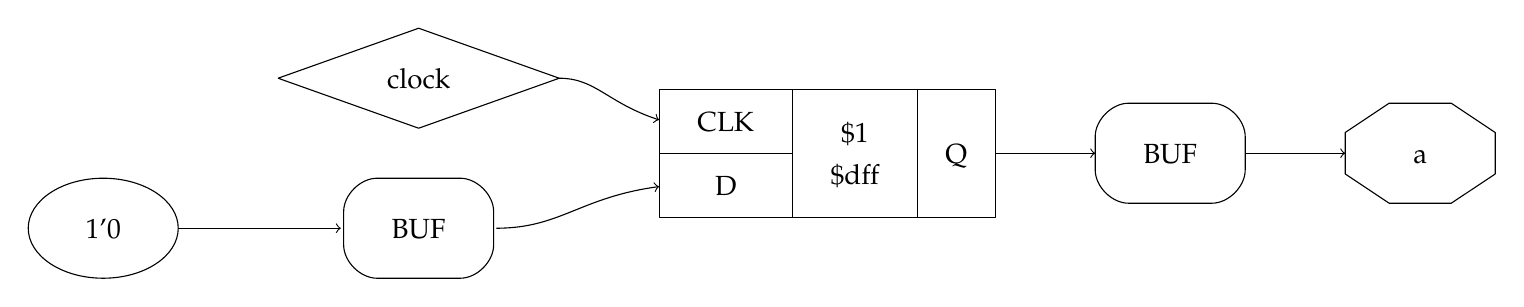
\begin{tikzpicture}[line join=bevel,anchor=base]%
\pgfsetcolor{black}
  % Edge: c8 -> x2
  \draw [->] (348.11bp,45.0bp) .. controls (360.11bp,45.0bp) and (365.36bp,45.0bp)  .. (384.11bp,45.0bp);
  % Edge: v0 -> x1
  \draw [->] (54.0bp,18.0bp) .. controls (76.161bp,18.0bp) and (84.168bp,18.0bp)  .. (112.55bp,18.0bp);
  % Edge: x2 -> n4
  \draw [->] (438.11bp,45.0bp) .. controls (450.11bp,45.0bp) and (455.36bp,45.0bp)  .. (474.11bp,45.0bp);
  % Edge: n3 -> c8
  \draw [->] (191.11bp,72.0bp) .. controls (204.38bp,72.0bp) and (208.27bp,63.207bp)  .. (227.11bp,57.0bp);
  % Edge: x1 -> c8
  \draw [->] (168.55bp,18.0bp) .. controls (191.64bp,18.0bp) and (198.45bp,29.078bp)  .. (227.11bp,33.0bp);
  % Node: x1
\begin{scope}
  \definecolor{strokecol}{rgb}{0.0,0.0,0.0};
  \pgfsetstrokecolor{strokecol}
  \draw (155.55bp,36.0bp) .. controls (155.55bp,36.0bp) and (125.55bp,36.0bp)  .. (125.55bp,36.0bp) .. controls (119.55bp,36.0bp) and (113.55bp,30.0bp)  .. (113.55bp,24.0bp) .. controls (113.55bp,24.0bp) and (113.55bp,12.0bp)  .. (113.55bp,12.0bp) .. controls (113.55bp,6.0bp) and (119.55bp,0.0bp)  .. (125.55bp,0.0bp) .. controls (125.55bp,0.0bp) and (155.55bp,0.0bp)  .. (155.55bp,0.0bp) .. controls (161.55bp,0.0bp) and (167.55bp,6.0bp)  .. (167.55bp,12.0bp) .. controls (167.55bp,12.0bp) and (167.55bp,24.0bp)  .. (167.55bp,24.0bp) .. controls (167.55bp,30.0bp) and (161.55bp,36.0bp)  .. (155.55bp,36.0bp);
  \draw (140.55bp,14.3bp) node {BUF};
\end{scope}
  % Node: v0
\begin{scope}
  \definecolor{strokecol}{rgb}{0.0,0.0,0.0};
  \pgfsetstrokecolor{strokecol}
  \draw (27.0bp,18.0bp) ellipse (27.0bp and 18.0bp);
  \draw (27.0bp,14.3bp) node {1'0};
\end{scope}
  % Node: c8
\begin{scope}
  \definecolor{strokecol}{rgb}{0.0,0.0,0.0};
  \pgfsetstrokecolor{strokecol}
  \draw (227.11bp,22.0bp) -- (227.11bp,68.0bp) -- (348.11bp,68.0bp) -- (348.11bp,22.0bp) -- cycle;
  \draw (227.11bp,45.0bp) -- (275.11bp,45.0bp);
  \draw (275.11bp,22.0bp) -- (275.11bp,68.0bp);
  \draw (320.11bp,22.0bp) -- (320.11bp,68.0bp);
  \draw (251.11bp,52.8bp) node {CLK};
  \draw (251.11bp,29.8bp) node {D};
  \draw (297.61bp,48.8bp) node {\$1};
  \draw (297.61bp,33.8bp) node {\$dff};
  \draw (334.11bp,41.3bp) node {Q};
\end{scope}
  % Node: x2
\begin{scope}
  \definecolor{strokecol}{rgb}{0.0,0.0,0.0};
  \pgfsetstrokecolor{strokecol}
  \draw (426.11bp,63.0bp) .. controls (426.11bp,63.0bp) and (396.11bp,63.0bp)  .. (396.11bp,63.0bp) .. controls (390.11bp,63.0bp) and (384.11bp,57.0bp)  .. (384.11bp,51.0bp) .. controls (384.11bp,51.0bp) and (384.11bp,39.0bp)  .. (384.11bp,39.0bp) .. controls (384.11bp,33.0bp) and (390.11bp,27.0bp)  .. (396.11bp,27.0bp) .. controls (396.11bp,27.0bp) and (426.11bp,27.0bp)  .. (426.11bp,27.0bp) .. controls (432.11bp,27.0bp) and (438.11bp,33.0bp)  .. (438.11bp,39.0bp) .. controls (438.11bp,39.0bp) and (438.11bp,51.0bp)  .. (438.11bp,51.0bp) .. controls (438.11bp,57.0bp) and (432.11bp,63.0bp)  .. (426.11bp,63.0bp);
  \draw (411.11bp,41.3bp) node {BUF};
\end{scope}
  % Node: n3
\begin{scope}
  \definecolor{strokecol}{rgb}{0.0,0.0,0.0};
  \pgfsetstrokecolor{strokecol}
  \draw (140.55bp,90.0bp) -- (89.95bp,72.0bp) -- (140.55bp,54.0bp) -- (191.16bp,72.0bp) -- cycle;
  \draw (140.55bp,68.3bp) node {clock};
\end{scope}
  % Node: n4
\begin{scope}
  \definecolor{strokecol}{rgb}{0.0,0.0,0.0};
  \pgfsetstrokecolor{strokecol}
  \draw (528.11bp,37.54bp) -- (528.11bp,52.46bp) -- (512.29bp,63.0bp) -- (489.92bp,63.0bp) -- (474.11bp,52.46bp) -- (474.11bp,37.54bp) -- (489.92bp,27.0bp) -- (512.29bp,27.0bp) -- cycle;
  \draw (501.11bp,41.3bp) node {a};
\end{scope}
\end{tikzpicture}}%

    \label{fig:netlistMotSync}
\end{figure}

\subsubsection{Nested synchronized assignment}
\leavevmode\begin{lstlisting}[style=vhdl, caption={Code for a nested synchronized
      bit assignment}, label={lst:motSyncNest}]
-- [...]
-- A and clock are both of type std_logic
architecture behv of adder is
   function rising_edge(c : in std_logic) return std_logic;
begin
   process(A) is
   begin
      if rising_edge(clock) then
         if rising_edge(clock) then
            A <= '0';
         end if;
      end if;
   end process;
end behv;
\end{lstlisting}
%
Listing \ref{lst:motSyncNest} contains an assignment that gets
doubly synchronized by the two enclosing if statements. Commercial
tools would probably report a warning or, in some contexts, an
error. Yodl, however, does not complain as standard \cite{IEEESYNTH}
does not explicitly forbids this kind of synthesis behavior
(cf. chapter 6.1). The
netlist in figure \ref{fig:netlistMotSyncNest} clearly shows the
result of such a nesting. As opposed to circuit
\ref{fig:netlistMotSync}, the nested version needs one additional
clock cycle for \VH{'0'} to appear on output \VH{A}.

\begin{figure}[p]
    \centering
    \caption{Netlist for the listing \ref{lst:motSyncNest}}
    \resizebox{\textwidth}{!}{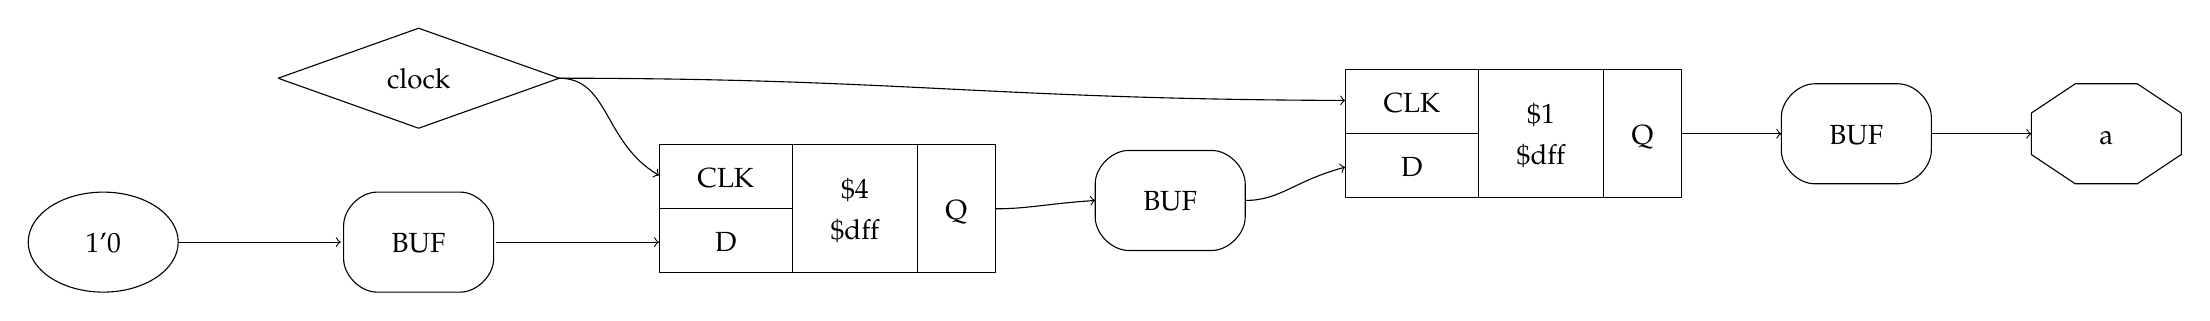
\begin{tikzpicture}[line join=bevel,anchor=base]%
\pgfsetcolor{black}
  % Edge: x3 -> n6
  \draw [->] (685.11bp,57.0bp) .. controls (697.11bp,57.0bp) and (702.36bp,57.0bp)  .. (721.11bp,57.0bp);
  % Edge: x1 -> c10
  \draw [->] (168.55bp,18.0bp) .. controls (190.71bp,18.0bp) and (198.72bp,18.0bp)  .. (227.11bp,18.0bp);
  % Edge: c10 -> x2
  \draw [->] (348.11bp,30.0bp) .. controls (360.15bp,30.0bp) and (365.35bp,31.688bp)  .. (384.11bp,33.0bp);
  % Edge: x2 -> c11
  \draw [->] (438.11bp,33.0bp) .. controls (450.89bp,33.0bp) and (455.29bp,39.891bp)  .. (474.11bp,45.0bp);
  % Edge: v0 -> x1
  \draw [->] (54.0bp,18.0bp) .. controls (76.161bp,18.0bp) and (84.168bp,18.0bp)  .. (112.55bp,18.0bp);
  % Edge: n5 -> c11
  \draw [->] (191.11bp,77.0bp) .. controls (313.49bp,77.0bp) and (346.49bp,69.432bp)  .. (474.11bp,69.0bp);
  % Edge: c11 -> x3
  \draw [->] (595.11bp,57.0bp) .. controls (607.11bp,57.0bp) and (612.36bp,57.0bp)  .. (631.11bp,57.0bp);
  % Edge: n5 -> c10
  \draw [->] (191.11bp,77.0bp) .. controls (209.24bp,77.0bp) and (206.94bp,53.895bp)  .. (227.11bp,42.0bp);
  % Node: x1
\begin{scope}
  \definecolor{strokecol}{rgb}{0.0,0.0,0.0};
  \pgfsetstrokecolor{strokecol}
  \draw (155.55bp,36.0bp) .. controls (155.55bp,36.0bp) and (125.55bp,36.0bp)  .. (125.55bp,36.0bp) .. controls (119.55bp,36.0bp) and (113.55bp,30.0bp)  .. (113.55bp,24.0bp) .. controls (113.55bp,24.0bp) and (113.55bp,12.0bp)  .. (113.55bp,12.0bp) .. controls (113.55bp,6.0bp) and (119.55bp,0.0bp)  .. (125.55bp,0.0bp) .. controls (125.55bp,0.0bp) and (155.55bp,0.0bp)  .. (155.55bp,0.0bp) .. controls (161.55bp,0.0bp) and (167.55bp,6.0bp)  .. (167.55bp,12.0bp) .. controls (167.55bp,12.0bp) and (167.55bp,24.0bp)  .. (167.55bp,24.0bp) .. controls (167.55bp,30.0bp) and (161.55bp,36.0bp)  .. (155.55bp,36.0bp);
  \draw (140.55bp,14.3bp) node {BUF};
\end{scope}
  % Node: v0
\begin{scope}
  \definecolor{strokecol}{rgb}{0.0,0.0,0.0};
  \pgfsetstrokecolor{strokecol}
  \draw (27.0bp,18.0bp) ellipse (27.0bp and 18.0bp);
  \draw (27.0bp,14.3bp) node {1'0};
\end{scope}
  % Node: x2
\begin{scope}
  \definecolor{strokecol}{rgb}{0.0,0.0,0.0};
  \pgfsetstrokecolor{strokecol}
  \draw (426.11bp,51.0bp) .. controls (426.11bp,51.0bp) and (396.11bp,51.0bp)  .. (396.11bp,51.0bp) .. controls (390.11bp,51.0bp) and (384.11bp,45.0bp)  .. (384.11bp,39.0bp) .. controls (384.11bp,39.0bp) and (384.11bp,27.0bp)  .. (384.11bp,27.0bp) .. controls (384.11bp,21.0bp) and (390.11bp,15.0bp)  .. (396.11bp,15.0bp) .. controls (396.11bp,15.0bp) and (426.11bp,15.0bp)  .. (426.11bp,15.0bp) .. controls (432.11bp,15.0bp) and (438.11bp,21.0bp)  .. (438.11bp,27.0bp) .. controls (438.11bp,27.0bp) and (438.11bp,39.0bp)  .. (438.11bp,39.0bp) .. controls (438.11bp,45.0bp) and (432.11bp,51.0bp)  .. (426.11bp,51.0bp);
  \draw (411.11bp,29.3bp) node {BUF};
\end{scope}
  % Node: x3
\begin{scope}
  \definecolor{strokecol}{rgb}{0.0,0.0,0.0};
  \pgfsetstrokecolor{strokecol}
  \draw (673.11bp,75.0bp) .. controls (673.11bp,75.0bp) and (643.11bp,75.0bp)  .. (643.11bp,75.0bp) .. controls (637.11bp,75.0bp) and (631.11bp,69.0bp)  .. (631.11bp,63.0bp) .. controls (631.11bp,63.0bp) and (631.11bp,51.0bp)  .. (631.11bp,51.0bp) .. controls (631.11bp,45.0bp) and (637.11bp,39.0bp)  .. (643.11bp,39.0bp) .. controls (643.11bp,39.0bp) and (673.11bp,39.0bp)  .. (673.11bp,39.0bp) .. controls (679.11bp,39.0bp) and (685.11bp,45.0bp)  .. (685.11bp,51.0bp) .. controls (685.11bp,51.0bp) and (685.11bp,63.0bp)  .. (685.11bp,63.0bp) .. controls (685.11bp,69.0bp) and (679.11bp,75.0bp)  .. (673.11bp,75.0bp);
  \draw (658.11bp,53.3bp) node {BUF};
\end{scope}
  % Node: c11
\begin{scope}
  \definecolor{strokecol}{rgb}{0.0,0.0,0.0};
  \pgfsetstrokecolor{strokecol}
  \draw (474.11bp,34.0bp) -- (474.11bp,80.0bp) -- (595.11bp,80.0bp) -- (595.11bp,34.0bp) -- cycle;
  \draw (474.11bp,57.0bp) -- (522.11bp,57.0bp);
  \draw (522.11bp,34.0bp) -- (522.11bp,80.0bp);
  \draw (567.11bp,34.0bp) -- (567.11bp,80.0bp);
  \draw (498.11bp,64.8bp) node {CLK};
  \draw (498.11bp,41.8bp) node {D};
  \draw (544.61bp,60.8bp) node {\$1};
  \draw (544.61bp,45.8bp) node {\$dff};
  \draw (581.11bp,53.3bp) node {Q};
\end{scope}
  % Node: c10
\begin{scope}
  \definecolor{strokecol}{rgb}{0.0,0.0,0.0};
  \pgfsetstrokecolor{strokecol}
  \draw (227.11bp,7.0bp) -- (227.11bp,53.0bp) -- (348.11bp,53.0bp) -- (348.11bp,7.0bp) -- cycle;
  \draw (227.11bp,30.0bp) -- (275.11bp,30.0bp);
  \draw (275.11bp,7.0bp) -- (275.11bp,53.0bp);
  \draw (320.11bp,7.0bp) -- (320.11bp,53.0bp);
  \draw (251.11bp,37.8bp) node {CLK};
  \draw (251.11bp,14.8bp) node {D};
  \draw (297.61bp,33.8bp) node {\$4};
  \draw (297.61bp,18.8bp) node {\$dff};
  \draw (334.11bp,26.3bp) node {Q};
\end{scope}
  % Node: n5
\begin{scope}
  \definecolor{strokecol}{rgb}{0.0,0.0,0.0};
  \pgfsetstrokecolor{strokecol}
  \draw (140.55bp,95.0bp) -- (89.95bp,77.0bp) -- (140.55bp,59.0bp) -- (191.16bp,77.0bp) -- cycle;
  \draw (140.55bp,73.3bp) node {clock};
\end{scope}
  % Node: n6
\begin{scope}
  \definecolor{strokecol}{rgb}{0.0,0.0,0.0};
  \pgfsetstrokecolor{strokecol}
  \draw (775.11bp,49.54bp) -- (775.11bp,64.46bp) -- (759.29bp,75.0bp) -- (736.92bp,75.0bp) -- (721.11bp,64.46bp) -- (721.11bp,49.54bp) -- (736.92bp,39.0bp) -- (759.29bp,39.0bp) -- cycle;
  \draw (748.11bp,53.3bp) node {a};
\end{scope}
\end{tikzpicture}}%

    \label{fig:netlistMotSyncNest}
\end{figure}

\subsubsection{Simple latched assignment}
\label{sec:SimpleLatchedAssign}
\leavevmode\begin{lstlisting}[style=vhdl, caption={Code for a simple latched bit
      assignment}, label={lst:motLatch}]
-- same libraries as above
-- A, B and C are of type std_logic
architecture behv of adder is
   function rising_edge(c : in std_logic) return boolean;
begin
   process(A) is
   begin
      if A = B then
         C <= '1';
      end if;
   end process;
end behv;
\end{lstlisting}
%
Level sensitive flip-flops are commonly called \emph{latch}. DFF's
only sample values at clock edge, whereas latches maintain a constant
connection between their inputs and outputs if the signal value is
either zero or one (cf. \cite{DIGITALTECHNIK}, 11.3). For instance,
suppose a latch is low-level
active. This latch would only interconnect its input and output only
if the enable input equals zero. DFF's also possess input pins like
\emph{enable}, but in this case those inputs are commonly called
\emph{clock}, because of the emphasis on clock edge synchronicity.

Listing \ref{lst:motLatch} contains a single if statement with an
ordinary condition on top of it. It does not have an else-path. As a
consequence, a register-like hardware cell must be used to handle the
case when the condition \VH{A = B} does not apply. If it does, \VH{C}
will be driven with the constant value of \VH{1}. Otherwise, the
previous value (in this case always \VH{1}) will be stored. Note how
\ref{fig:netlistMotLatch} connects the netlist for the condition
directly with the \emph{EN} input of the latch.

In digital circuits, particularly in synchronous circuits, the usage
of latches is mostly unwanted as latches can't generally be used for
feedback assignments like: \VH{A <= A + 1;}
However, this is a topic far beyond the scope of this work. References
for further reading are 3.6.2, 3.6.1 and, most importantly 3.4 from
\cite{VHDLSYNTHESE}.

\begin{figure}[p]
    \centering
    \caption{Netlist for listing \ref{lst:motLatch}}
    \resizebox{\textwidth}{!}{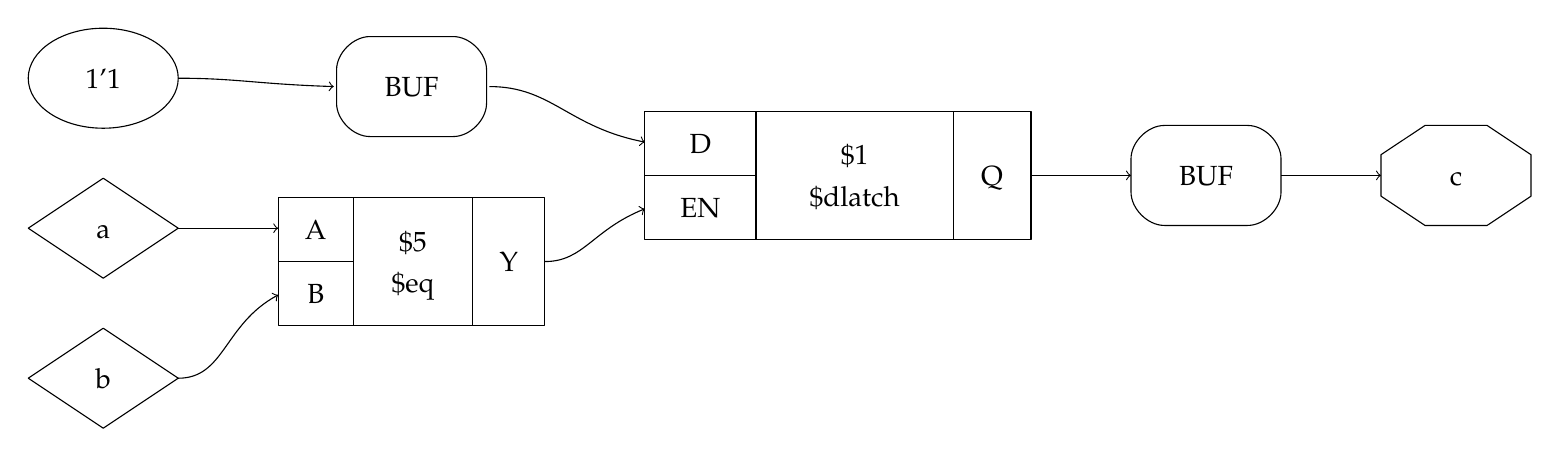
\begin{tikzpicture}[line join=bevel,anchor=base]%
\pgfsetcolor{black}
  % Edge: n6 -> c10
  \draw [->] (54.0bp,72.0bp) .. controls (66.0bp,72.0bp) and (71.25bp,72.0bp)  .. (90.0bp,72.0bp);
  % Edge: x2 -> n4
  \draw [->] (451.0bp,91.0bp) .. controls (463.0bp,91.0bp) and (468.25bp,91.0bp)  .. (487.0bp,91.0bp);
  % Edge: v0 -> x1
  \draw [->] (54.0bp,126.0bp) .. controls (75.03bp,126.0bp) and (82.695bp,123.86bp)  .. (110.0bp,123.0bp);
  % Edge: c14 -> x2
  \draw [->] (361.0bp,91.0bp) .. controls (373.0bp,91.0bp) and (378.25bp,91.0bp)  .. (397.0bp,91.0bp);
  % Edge: x1 -> c14
  \draw [->] (166.0bp,123.0bp) .. controls (188.51bp,123.0bp) and (194.13bp,108.5bp)  .. (222.0bp,103.0bp);
  % Edge: c10 -> c14
  \draw [->] (186.0bp,60.0bp) .. controls (199.99bp,60.0bp) and (203.05bp,71.366bp)  .. (222.0bp,79.0bp);
  % Edge: n5 -> c10
  \draw [->] (54.0bp,18.0bp) .. controls (70.759bp,18.0bp) and (70.371bp,37.426bp)  .. (90.0bp,48.0bp);
  % Node: x1
\begin{scope}
  \definecolor{strokecol}{rgb}{0.0,0.0,0.0};
  \pgfsetstrokecolor{strokecol}
  \draw (153.0bp,141.0bp) .. controls (153.0bp,141.0bp) and (123.0bp,141.0bp)  .. (123.0bp,141.0bp) .. controls (117.0bp,141.0bp) and (111.0bp,135.0bp)  .. (111.0bp,129.0bp) .. controls (111.0bp,129.0bp) and (111.0bp,117.0bp)  .. (111.0bp,117.0bp) .. controls (111.0bp,111.0bp) and (117.0bp,105.0bp)  .. (123.0bp,105.0bp) .. controls (123.0bp,105.0bp) and (153.0bp,105.0bp)  .. (153.0bp,105.0bp) .. controls (159.0bp,105.0bp) and (165.0bp,111.0bp)  .. (165.0bp,117.0bp) .. controls (165.0bp,117.0bp) and (165.0bp,129.0bp)  .. (165.0bp,129.0bp) .. controls (165.0bp,135.0bp) and (159.0bp,141.0bp)  .. (153.0bp,141.0bp);
  \draw (138.0bp,119.3bp) node {BUF};
\end{scope}
  % Node: v0
\begin{scope}
  \definecolor{strokecol}{rgb}{0.0,0.0,0.0};
  \pgfsetstrokecolor{strokecol}
  \draw (27.0bp,126.0bp) ellipse (27.0bp and 18.0bp);
  \draw (27.0bp,122.3bp) node {1'1};
\end{scope}
  % Node: x2
\begin{scope}
  \definecolor{strokecol}{rgb}{0.0,0.0,0.0};
  \pgfsetstrokecolor{strokecol}
  \draw (439.0bp,109.0bp) .. controls (439.0bp,109.0bp) and (409.0bp,109.0bp)  .. (409.0bp,109.0bp) .. controls (403.0bp,109.0bp) and (397.0bp,103.0bp)  .. (397.0bp,97.0bp) .. controls (397.0bp,97.0bp) and (397.0bp,85.0bp)  .. (397.0bp,85.0bp) .. controls (397.0bp,79.0bp) and (403.0bp,73.0bp)  .. (409.0bp,73.0bp) .. controls (409.0bp,73.0bp) and (439.0bp,73.0bp)  .. (439.0bp,73.0bp) .. controls (445.0bp,73.0bp) and (451.0bp,79.0bp)  .. (451.0bp,85.0bp) .. controls (451.0bp,85.0bp) and (451.0bp,97.0bp)  .. (451.0bp,97.0bp) .. controls (451.0bp,103.0bp) and (445.0bp,109.0bp)  .. (439.0bp,109.0bp);
  \draw (424.0bp,87.3bp) node {BUF};
\end{scope}
  % Node: c10
\begin{scope}
  \definecolor{strokecol}{rgb}{0.0,0.0,0.0};
  \pgfsetstrokecolor{strokecol}
  \draw (90.0bp,37.0bp) -- (90.0bp,83.0bp) -- (186.0bp,83.0bp) -- (186.0bp,37.0bp) -- cycle;
  \draw (90.0bp,60.0bp) -- (117.0bp,60.0bp);
  \draw (117.0bp,37.0bp) -- (117.0bp,83.0bp);
  \draw (160.0bp,37.0bp) -- (160.0bp,83.0bp);
  \draw (103.5bp,67.8bp) node {A};
  \draw (103.5bp,44.8bp) node {B};
  \draw (138.5bp,63.8bp) node {\$5};
  \draw (138.5bp,48.8bp) node {\$eq};
  \draw (173.0bp,56.3bp) node {Y};
\end{scope}
  % Node: n4
\begin{scope}
  \definecolor{strokecol}{rgb}{0.0,0.0,0.0};
  \pgfsetstrokecolor{strokecol}
  \draw (541.0bp,83.54bp) -- (541.0bp,98.46bp) -- (525.18bp,109.0bp) -- (502.82bp,109.0bp) -- (487.0bp,98.46bp) -- (487.0bp,83.54bp) -- (502.82bp,73.0bp) -- (525.18bp,73.0bp) -- cycle;
  \draw (514.0bp,87.3bp) node {c};
\end{scope}
  % Node: n5
\begin{scope}
  \definecolor{strokecol}{rgb}{0.0,0.0,0.0};
  \pgfsetstrokecolor{strokecol}
  \draw (27.0bp,36.0bp) -- (0.0bp,18.0bp) -- (27.0bp,0.0bp) -- (54.0bp,18.0bp) -- cycle;
  \draw (27.0bp,14.3bp) node {b};
\end{scope}
  % Node: n6
\begin{scope}
  \definecolor{strokecol}{rgb}{0.0,0.0,0.0};
  \pgfsetstrokecolor{strokecol}
  \draw (27.0bp,90.0bp) -- (0.0bp,72.0bp) -- (27.0bp,54.0bp) -- (54.0bp,72.0bp) -- cycle;
  \draw (27.0bp,68.3bp) node {a};
\end{scope}
  % Node: c14
\begin{scope}
  \definecolor{strokecol}{rgb}{0.0,0.0,0.0};
  \pgfsetstrokecolor{strokecol}
  \draw (222.0bp,68.0bp) -- (222.0bp,114.0bp) -- (361.0bp,114.0bp) -- (361.0bp,68.0bp) -- cycle;
  \draw (222.0bp,91.0bp) -- (262.0bp,91.0bp);
  \draw (262.0bp,68.0bp) -- (262.0bp,114.0bp);
  \draw (333.0bp,68.0bp) -- (333.0bp,114.0bp);
  \draw (242.0bp,98.8bp) node {D};
  \draw (242.0bp,75.8bp) node {EN};
  \draw (297.5bp,94.8bp) node {\$1};
  \draw (297.5bp,79.8bp) node {\$dlatch};
  \draw (347.0bp,87.3bp) node {Q};
\end{scope}
\end{tikzpicture}}%

    \label{fig:netlistMotLatch}
\end{figure}

\subsubsection{Nested, latched assignment}
\leavevmode\begin{lstlisting}[style=vhdl, caption={Code for a nested latched bit
      assignment}, label={lst:motLatchNest}]
-- [...]
-- same preamble as above
   process(A) is
   begin
      if A = B then
         if not A then
             C <= '1';
         end if;
      end if;
   end process;
end behv;
\end{lstlisting}
%
Analogous to the snippet in listing \ref{lst:motSyncNest}, latches can
be cascaded too. The relationship between the netlists
\ref{fig:netlistMotLatchNest} and
\ref{fig:netlistMotLatch} exactly correspond to
\ref{fig:netlistMotSync} and
\ref{fig:netlistMotSyncNest}. Consequently, a description of if would
be redundant.

\begin{figure}[p]
    \centering
    \caption{Netlist for listing \ref{lst:motLatchNest}}
    \resizebox{\textwidth}{!}{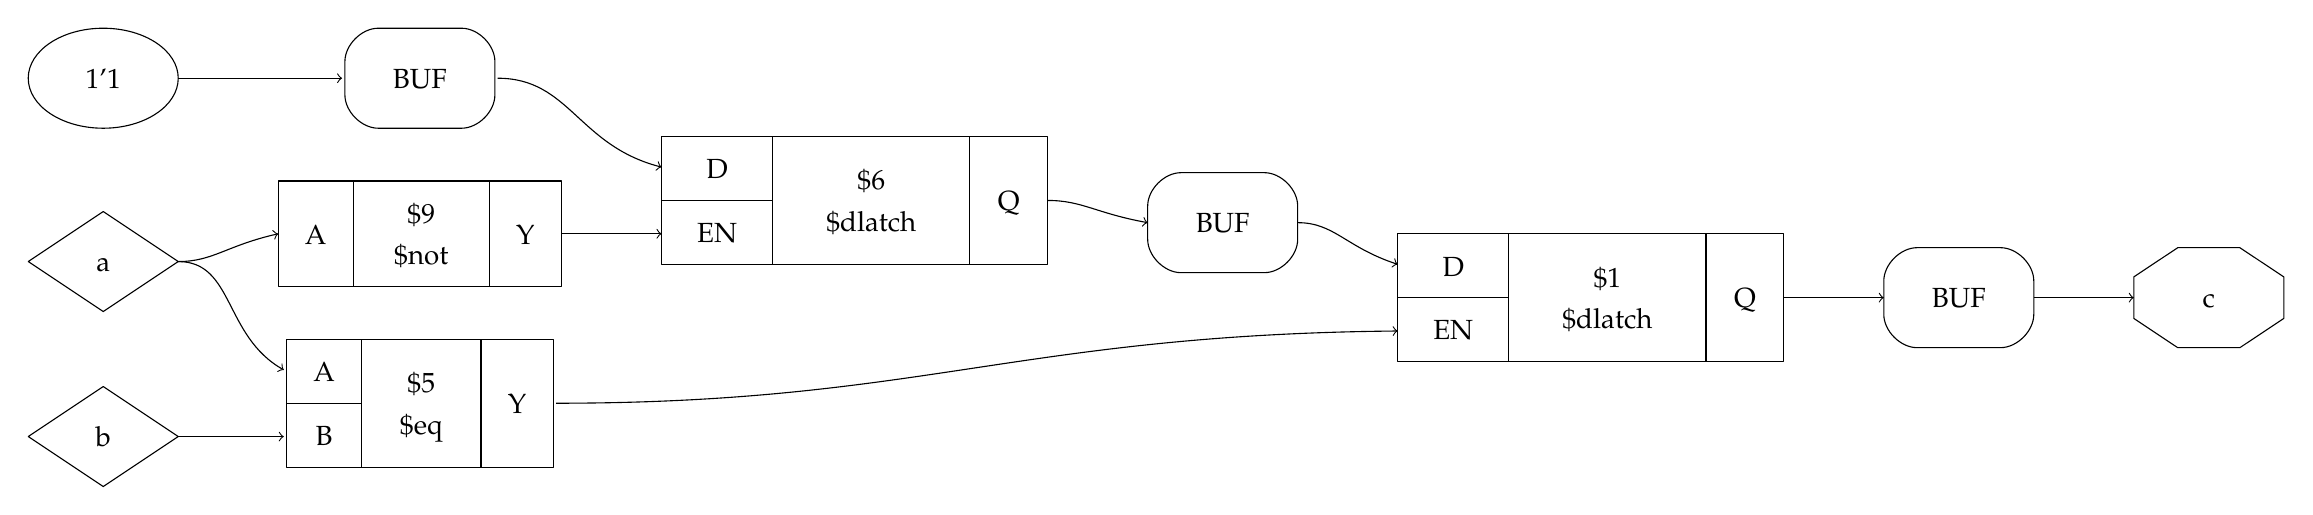
\begin{tikzpicture}[line join=bevel,anchor=base]%
\pgfsetcolor{black}
  % Edge: c12 -> c16
  \draw [->] (192.0bp,91.0bp) .. controls (204.0bp,91.0bp) and (209.25bp,91.0bp)  .. (228.0bp,91.0bp);
  % Edge: c18 -> c19
  \draw [->] (190.0bp,30.0bp) .. controls (321.73bp,30.0bp) and (356.11bp,54.696bp)  .. (493.0bp,56.0bp);
  % Edge: n9 -> c18
  \draw [->] (54.0bp,81.0bp) .. controls (74.041bp,81.0bp) and (70.353bp,54.254bp)  .. (92.0bp,42.0bp);
  % Edge: x2 -> c19
  \draw [->] (457.0bp,95.0bp) .. controls (470.27bp,95.0bp) and (474.16bp,86.207bp)  .. (493.0bp,80.0bp);
  % Edge: c19 -> x3
  \draw [->] (632.0bp,68.0bp) .. controls (644.0bp,68.0bp) and (649.25bp,68.0bp)  .. (668.0bp,68.0bp);
  % Edge: x3 -> n7
  \draw [->] (722.0bp,68.0bp) .. controls (734.0bp,68.0bp) and (739.25bp,68.0bp)  .. (758.0bp,68.0bp);
  % Edge: v0 -> x1
  \draw [->] (54.0bp,147.0bp) .. controls (76.535bp,147.0bp) and (84.545bp,147.0bp)  .. (113.0bp,147.0bp);
  % Edge: n9 -> c12
  \draw [->] (54.0bp,81.0bp) .. controls (66.584bp,81.0bp) and (71.233bp,86.743bp)  .. (90.0bp,91.0bp);
  % Edge: c16 -> x2
  \draw [->] (367.0bp,103.0bp) .. controls (379.42bp,103.0bp) and (384.28bp,98.406bp)  .. (403.0bp,95.0bp);
  % Edge: n8 -> c18
  \draw [->] (54.0bp,18.0bp) .. controls (66.931bp,18.0bp) and (72.436bp,18.0bp)  .. (92.0bp,18.0bp);
  % Edge: x1 -> c16
  \draw [->] (169.0bp,147.0bp) .. controls (194.99bp,147.0bp) and (197.83bp,122.72bp)  .. (228.0bp,115.0bp);
  % Node: v0
\begin{scope}
  \definecolor{strokecol}{rgb}{0.0,0.0,0.0};
  \pgfsetstrokecolor{strokecol}
  \draw (27.0bp,147.0bp) ellipse (27.0bp and 18.0bp);
  \draw (27.0bp,143.3bp) node {1'1};
\end{scope}
  % Node: n8
\begin{scope}
  \definecolor{strokecol}{rgb}{0.0,0.0,0.0};
  \pgfsetstrokecolor{strokecol}
  \draw (27.0bp,36.0bp) -- (0.0bp,18.0bp) -- (27.0bp,0.0bp) -- (54.0bp,18.0bp) -- cycle;
  \draw (27.0bp,14.3bp) node {b};
\end{scope}
  % Node: n9
\begin{scope}
  \definecolor{strokecol}{rgb}{0.0,0.0,0.0};
  \pgfsetstrokecolor{strokecol}
  \draw (27.0bp,99.0bp) -- (0.0bp,81.0bp) -- (27.0bp,63.0bp) -- (54.0bp,81.0bp) -- cycle;
  \draw (27.0bp,77.3bp) node {a};
\end{scope}
  % Node: c19
\begin{scope}
  \definecolor{strokecol}{rgb}{0.0,0.0,0.0};
  \pgfsetstrokecolor{strokecol}
  \draw (493.0bp,45.0bp) -- (493.0bp,91.0bp) -- (632.0bp,91.0bp) -- (632.0bp,45.0bp) -- cycle;
  \draw (493.0bp,68.0bp) -- (533.0bp,68.0bp);
  \draw (533.0bp,45.0bp) -- (533.0bp,91.0bp);
  \draw (604.0bp,45.0bp) -- (604.0bp,91.0bp);
  \draw (513.0bp,75.8bp) node {D};
  \draw (513.0bp,52.8bp) node {EN};
  \draw (568.5bp,71.8bp) node {\$1};
  \draw (568.5bp,56.8bp) node {\$dlatch};
  \draw (618.0bp,64.3bp) node {Q};
\end{scope}
  % Node: c18
\begin{scope}
  \definecolor{strokecol}{rgb}{0.0,0.0,0.0};
  \pgfsetstrokecolor{strokecol}
  \draw (93.0bp,7.0bp) -- (93.0bp,53.0bp) -- (189.0bp,53.0bp) -- (189.0bp,7.0bp) -- cycle;
  \draw (93.0bp,30.0bp) -- (120.0bp,30.0bp);
  \draw (120.0bp,7.0bp) -- (120.0bp,53.0bp);
  \draw (163.0bp,7.0bp) -- (163.0bp,53.0bp);
  \draw (106.5bp,37.8bp) node {A};
  \draw (106.5bp,14.8bp) node {B};
  \draw (141.5bp,33.8bp) node {\$5};
  \draw (141.5bp,18.8bp) node {\$eq};
  \draw (176.0bp,26.3bp) node {Y};
\end{scope}
  % Node: x3
\begin{scope}
  \definecolor{strokecol}{rgb}{0.0,0.0,0.0};
  \pgfsetstrokecolor{strokecol}
  \draw (710.0bp,86.0bp) .. controls (710.0bp,86.0bp) and (680.0bp,86.0bp)  .. (680.0bp,86.0bp) .. controls (674.0bp,86.0bp) and (668.0bp,80.0bp)  .. (668.0bp,74.0bp) .. controls (668.0bp,74.0bp) and (668.0bp,62.0bp)  .. (668.0bp,62.0bp) .. controls (668.0bp,56.0bp) and (674.0bp,50.0bp)  .. (680.0bp,50.0bp) .. controls (680.0bp,50.0bp) and (710.0bp,50.0bp)  .. (710.0bp,50.0bp) .. controls (716.0bp,50.0bp) and (722.0bp,56.0bp)  .. (722.0bp,62.0bp) .. controls (722.0bp,62.0bp) and (722.0bp,74.0bp)  .. (722.0bp,74.0bp) .. controls (722.0bp,80.0bp) and (716.0bp,86.0bp)  .. (710.0bp,86.0bp);
  \draw (695.0bp,64.3bp) node {BUF};
\end{scope}
  % Node: x2
\begin{scope}
  \definecolor{strokecol}{rgb}{0.0,0.0,0.0};
  \pgfsetstrokecolor{strokecol}
  \draw (445.0bp,113.0bp) .. controls (445.0bp,113.0bp) and (415.0bp,113.0bp)  .. (415.0bp,113.0bp) .. controls (409.0bp,113.0bp) and (403.0bp,107.0bp)  .. (403.0bp,101.0bp) .. controls (403.0bp,101.0bp) and (403.0bp,89.0bp)  .. (403.0bp,89.0bp) .. controls (403.0bp,83.0bp) and (409.0bp,77.0bp)  .. (415.0bp,77.0bp) .. controls (415.0bp,77.0bp) and (445.0bp,77.0bp)  .. (445.0bp,77.0bp) .. controls (451.0bp,77.0bp) and (457.0bp,83.0bp)  .. (457.0bp,89.0bp) .. controls (457.0bp,89.0bp) and (457.0bp,101.0bp)  .. (457.0bp,101.0bp) .. controls (457.0bp,107.0bp) and (451.0bp,113.0bp)  .. (445.0bp,113.0bp);
  \draw (430.0bp,91.3bp) node {BUF};
\end{scope}
  % Node: c12
\begin{scope}
  \definecolor{strokecol}{rgb}{0.0,0.0,0.0};
  \pgfsetstrokecolor{strokecol}
  \draw (90.0bp,72.0bp) -- (90.0bp,110.0bp) -- (192.0bp,110.0bp) -- (192.0bp,72.0bp) -- cycle;
  \draw (117.0bp,72.0bp) -- (117.0bp,110.0bp);
  \draw (166.0bp,72.0bp) -- (166.0bp,110.0bp);
  \draw (103.5bp,87.3bp) node {A};
  \draw (141.5bp,94.8bp) node {\$9};
  \draw (141.5bp,79.8bp) node {\$not};
  \draw (179.0bp,87.3bp) node {Y};
\end{scope}
  % Node: x1
\begin{scope}
  \definecolor{strokecol}{rgb}{0.0,0.0,0.0};
  \pgfsetstrokecolor{strokecol}
  \draw (156.0bp,165.0bp) .. controls (156.0bp,165.0bp) and (126.0bp,165.0bp)  .. (126.0bp,165.0bp) .. controls (120.0bp,165.0bp) and (114.0bp,159.0bp)  .. (114.0bp,153.0bp) .. controls (114.0bp,153.0bp) and (114.0bp,141.0bp)  .. (114.0bp,141.0bp) .. controls (114.0bp,135.0bp) and (120.0bp,129.0bp)  .. (126.0bp,129.0bp) .. controls (126.0bp,129.0bp) and (156.0bp,129.0bp)  .. (156.0bp,129.0bp) .. controls (162.0bp,129.0bp) and (168.0bp,135.0bp)  .. (168.0bp,141.0bp) .. controls (168.0bp,141.0bp) and (168.0bp,153.0bp)  .. (168.0bp,153.0bp) .. controls (168.0bp,159.0bp) and (162.0bp,165.0bp)  .. (156.0bp,165.0bp);
  \draw (141.0bp,143.3bp) node {BUF};
\end{scope}
  % Node: c16
\begin{scope}
  \definecolor{strokecol}{rgb}{0.0,0.0,0.0};
  \pgfsetstrokecolor{strokecol}
  \draw (228.0bp,80.0bp) -- (228.0bp,126.0bp) -- (367.0bp,126.0bp) -- (367.0bp,80.0bp) -- cycle;
  \draw (228.0bp,103.0bp) -- (268.0bp,103.0bp);
  \draw (268.0bp,80.0bp) -- (268.0bp,126.0bp);
  \draw (339.0bp,80.0bp) -- (339.0bp,126.0bp);
  \draw (248.0bp,110.8bp) node {D};
  \draw (248.0bp,87.8bp) node {EN};
  \draw (303.5bp,106.8bp) node {\$6};
  \draw (303.5bp,91.8bp) node {\$dlatch};
  \draw (353.0bp,99.3bp) node {Q};
\end{scope}
  % Node: n7
\begin{scope}
  \definecolor{strokecol}{rgb}{0.0,0.0,0.0};
  \pgfsetstrokecolor{strokecol}
  \draw (812.0bp,60.54bp) -- (812.0bp,75.46bp) -- (796.18bp,86.0bp) -- (773.82bp,86.0bp) -- (758.0bp,75.46bp) -- (758.0bp,60.54bp) -- (773.82bp,50.0bp) -- (796.18bp,50.0bp) -- cycle;
  \draw (785.0bp,64.3bp) node {c};
\end{scope}
\end{tikzpicture}}%

    \label{fig:netlistMotLatchNest}
\end{figure}

\subsubsection{Simple case statement}
\leavevmode\begin{lstlisting}[style=vhdl, caption={Code for a simple case
      statement}, label={lst:caseStmt}]
-- same libraries as before
-- A is a std_logic and baz a std_logic_vector(2 downto 0)
architecture behv of caseT is
begin
   process(A) is
   begin
      case baz is
         when "000" => A <= '0';
         when "001" => A <= '1';
         when "010" => A <= '1';
         when "011" => A <= '1';
         when "100" => A <= '0';
         when "101" => A <= '1';
         when "110" => A <= '1';
         when "111" => A <= '1';
      end case;
   end process;
end behv;
\end{lstlisting}
%
VHDL's case statement's are particularly interesting for synthesis
because all test from all choices must be performed parallel in
hardware. Listing \ref{lst:caseStmt} shows a simple example of a
case statement being used to model a 3-muxer. The fact that,
for instance, \VH{A <= '0'}, could be replaced by an arbitrary
sequence of sequential statements shall be neglected for now.

The code from \ref{lst:caseStmt} can be interpreted as: ``if \VH{baz} equals
the signal vector containing \VH{000}, \VH{A} shall be driven by
\VH{'0'} \ldots''. The netlist \ref{fig:netlistCaseStmt} presents an
implementation of this behaviour. Note that \$-mux cells are
equivalent to the abstract multiplexers from section
\ref{sec:semOfCase}. Figure \ref{fig:netlistCaseStmt} shows that each
muxer has three inputs and a single output. Analogous to the the muxer semantics
from \ref{sec:semOfCase}, \VH{A} gets selected if \VH{S} equals
zero, otherwise \VH{B}.

Note that nodes with rounded corners connecting the various muxer
selectors with the signal \VH{baz} show which bit is being connected
by the respective edge. For example \VH{2:2 - 0:0} means that the
slice \VH{2:2} (just one bit) is connected to the zeroth bit on the
other side.

\begin{figure}[p]
    \centering
    \caption{Netlist for listing \ref{lst:caseStmt}}
    \resizebox{\textwidth}{!}{\begin{tikzpicture}[line join=bevel,anchor=base]%
\pgfsetcolor{black}
  % Edge: c26 -> c28
  \draw [->] (476.37bp,269.0bp) .. controls (532.34bp,269.0bp) and (462.93bp,382.31bp)  .. (512.37bp,399.0bp);
  % Edge: v18 -> x19
  \draw [->] (65.685bp,182.0bp) .. controls (86.38bp,182.0bp) and (93.979bp,182.0bp)  .. (120.87bp,182.0bp);
  % Edge: n16 -> x6
  \draw [->] (75.371bp,376.0bp) .. controls (208.57bp,376.0bp) and (244.4bp,376.0bp)  .. (382.87bp,376.0bp);
  % Edge: x13 -> c24
  \draw [->] (176.87bp,570.0bp) .. controls (199.8bp,570.0bp) and (197.15bp,540.99bp)  .. (222.37bp,530.0bp);
  % Edge: x5 -> c27
  \draw [open diamond-open diamond] (315.87bp,427.0bp) .. controls (338.24bp,427.9bp) and (344.91bp,429.09bp)  .. (367.37bp,430.0bp);
  % Edge: x19 -> c23
  \draw [->] (176.87bp,182.0bp) .. controls (211.9bp,182.0bp) and (189.24bp,242.54bp)  .. (222.37bp,257.0bp);
  % Edge: c23 -> c26
  \draw [->] (331.37bp,257.0bp) .. controls (349.5bp,257.0bp) and (347.2bp,280.11bp)  .. (367.37bp,292.0bp);
  % Edge: c25 -> c27
  \draw [->] (331.37bp,664.0bp) .. controls (412.62bp,664.0bp) and (293.91bp,492.51bp)  .. (367.37bp,476.0bp);
  % Edge: n16 -> x3
  \draw [->] (75.371bp,376.0bp) .. controls (127.35bp,376.0bp) and (65.473bp,591.22bp)  .. (111.37bp,625.0bp);
  % Edge: x9 -> n17
  \draw [->] (711.37bp,399.0bp) .. controls (723.37bp,399.0bp) and (728.62bp,399.0bp)  .. (747.37bp,399.0bp);
  % Edge: v22 -> x23
  \draw [->] (65.685bp,18.0bp) .. controls (86.38bp,18.0bp) and (93.979bp,18.0bp)  .. (120.87bp,18.0bp);
  % Edge: v12 -> x13
  \draw [->] (65.685bp,570.0bp) .. controls (86.38bp,570.0bp) and (93.979bp,570.0bp)  .. (120.87bp,570.0bp);
  % Edge: c24 -> c27
  \draw [->] (331.37bp,507.0bp) .. controls (355.93bp,507.0bp) and (343.85bp,467.84bp)  .. (367.37bp,453.0bp);
  % Edge: x1 -> c23
  \draw [open diamond-open diamond] (186.37bp,237.0bp) .. controls (202.67bp,235.82bp) and (206.1bp,235.18bp)  .. (222.37bp,234.0bp);
  % Edge: c27 -> c28
  \draw [->] (476.37bp,453.0bp) .. controls (493.36bp,453.0bp) and (492.65bp,432.93bp)  .. (512.37bp,422.0bp);
  % Edge: x17 -> c25
  \draw [->] (176.87bp,680.0bp) .. controls (194.46bp,680.0bp) and (199.38bp,669.23bp)  .. (222.37bp,664.0bp);
  % Edge: x2 -> c24
  \draw [open diamond-open diamond] (186.37bp,461.0bp) .. controls (202.94bp,469.23bp) and (205.85bp,475.84bp)  .. (222.37bp,484.0bp);
  % Edge: x3 -> c25
  \draw [open diamond-open diamond] (186.37bp,625.0bp) .. controls (202.73bp,631.01bp) and (206.01bp,634.99bp)  .. (222.37bp,641.0bp);
  % Edge: n16 -> x0
  \draw [->] (75.371bp,376.0bp) .. controls (139.47bp,376.0bp) and (53.959bp,105.23bp)  .. (111.37bp,73.0bp);
  % Edge: v20 -> x21
  \draw [->] (65.685bp,516.0bp) .. controls (86.38bp,516.0bp) and (93.979bp,516.0bp)  .. (120.87bp,516.0bp);
  % Edge: n16 -> x4
  \draw [->] (75.371bp,376.0bp) .. controls (92.538bp,376.0bp) and (95.038bp,367.29bp)  .. (111.37bp,362.0bp) .. controls (163.3bp,345.19bp) and (178.02bp,330.84bp)  .. (237.87bp,329.0bp);
  % Edge: n16 -> x2
  \draw [->] (75.371bp,376.0bp) .. controls (112.23bp,376.0bp) and (78.801bp,444.61bp)  .. (111.37bp,461.0bp);
  % Edge: c22 -> c26
  \draw [->] (331.37bp,101.0bp) .. controls (403.85bp,101.0bp) and (302.37bp,252.37bp)  .. (367.37bp,269.0bp);
  % Edge: n16 -> x1
  \draw [->] (75.371bp,376.0bp) .. controls (135.32bp,376.0bp) and (58.081bp,253.32bp)  .. (111.37bp,237.0bp);
  % Edge: x8 -> c25
  \draw [->] (176.87bp,734.0bp) .. controls (201.86bp,734.0bp) and (196.03bp,699.29bp)  .. (222.37bp,687.0bp);
  % Edge: v10 -> x11
  \draw [->] (65.685bp,292.0bp) .. controls (86.38bp,292.0bp) and (93.979bp,292.0bp)  .. (120.87bp,292.0bp);
  % Edge: n16 -> x5
  \draw [->] (75.371bp,376.0bp) .. controls (92.538bp,376.0bp) and (95.117bp,384.47bp)  .. (111.37bp,390.0bp) .. controls (163.47bp,407.71bp) and (177.63bp,424.8bp)  .. (237.87bp,427.0bp);
  % Edge: x23 -> c22
  \draw [->] (176.87bp,18.0bp) .. controls (215.0bp,18.0bp) and (186.84bp,86.167bp)  .. (222.37bp,101.0bp);
  % Edge: x15 -> c22
  \draw [->] (176.87bp,128.0bp) .. controls (193.36bp,128.0bp) and (199.69bp,125.36bp)  .. (222.37bp,124.0bp);
  % Edge: c28 -> x9
  \draw [->] (621.37bp,399.0bp) .. controls (633.37bp,399.0bp) and (638.62bp,399.0bp)  .. (657.37bp,399.0bp);
  % Edge: x6 -> c28
  \draw [open diamond-open diamond] (460.87bp,376.0bp) .. controls (483.23bp,376.0bp) and (489.92bp,376.0bp)  .. (512.37bp,376.0bp);
  % Edge: x21 -> c24
  \draw [->] (176.87bp,516.0bp) .. controls (193.62bp,516.0bp) and (199.58bp,510.06bp)  .. (222.37bp,507.0bp);
  % Edge: v16 -> x17
  \draw [->] (65.685bp,680.0bp) .. controls (86.38bp,680.0bp) and (93.979bp,680.0bp)  .. (120.87bp,680.0bp);
  % Edge: v14 -> x15
  \draw [->] (65.685bp,128.0bp) .. controls (86.38bp,128.0bp) and (93.979bp,128.0bp)  .. (120.87bp,128.0bp);
  % Edge: x0 -> c22
  \draw [open diamond-open diamond] (186.37bp,73.0bp) .. controls (202.62bp,74.938bp) and (206.13bp,76.066bp)  .. (222.37bp,78.0bp);
  % Edge: x4 -> c26
  \draw [open diamond-open diamond] (315.87bp,329.0bp) .. controls (349.23bp,313.11bp) and (333.98bp,261.53bp)  .. (367.37bp,246.0bp);
  % Edge: v7 -> x8
  \draw [->] (65.685bp,734.0bp) .. controls (86.38bp,734.0bp) and (93.979bp,734.0bp)  .. (120.87bp,734.0bp);
  % Edge: x11 -> c23
  \draw [->] (176.87bp,292.0bp) .. controls (193.86bp,292.0bp) and (199.47bp,284.08bp)  .. (222.37bp,280.0bp);
  % Node: v18
\begin{scope}
  \definecolor{strokecol}{rgb}{0.0,0.0,0.0};
  \pgfsetstrokecolor{strokecol}
  \draw (37.69bp,182.0bp) ellipse (27.0bp and 18.0bp);
  \draw (37.69bp,178.3bp) node {1'1};
\end{scope}
  % Node: n16
\begin{scope}
  \definecolor{strokecol}{rgb}{0.0,0.0,0.0};
  \pgfsetstrokecolor{strokecol}
  \draw (37.69bp,394.0bp) -- (-0.19bp,376.0bp) -- (37.69bp,358.0bp) -- (75.56bp,376.0bp) -- cycle;
  \draw (37.69bp,372.3bp) node {baz};
\end{scope}
  % Node: n17
\begin{scope}
  \definecolor{strokecol}{rgb}{0.0,0.0,0.0};
  \pgfsetstrokecolor{strokecol}
  \draw (801.37bp,391.54bp) -- (801.37bp,406.46bp) -- (785.55bp,417.0bp) -- (763.19bp,417.0bp) -- (747.37bp,406.46bp) -- (747.37bp,391.54bp) -- (763.19bp,381.0bp) -- (785.55bp,381.0bp) -- cycle;
  \draw (774.37bp,395.3bp) node {a};
\end{scope}
  % Node: v12
\begin{scope}
  \definecolor{strokecol}{rgb}{0.0,0.0,0.0};
  \pgfsetstrokecolor{strokecol}
  \draw (37.69bp,570.0bp) ellipse (27.0bp and 18.0bp);
  \draw (37.69bp,566.3bp) node {1'1};
\end{scope}
  % Node: v10
\begin{scope}
  \definecolor{strokecol}{rgb}{0.0,0.0,0.0};
  \pgfsetstrokecolor{strokecol}
  \draw (37.69bp,292.0bp) ellipse (27.0bp and 18.0bp);
  \draw (37.69bp,288.3bp) node {1'1};
\end{scope}
  % Node: v16
\begin{scope}
  \definecolor{strokecol}{rgb}{0.0,0.0,0.0};
  \pgfsetstrokecolor{strokecol}
  \draw (37.69bp,680.0bp) ellipse (27.0bp and 18.0bp);
  \draw (37.69bp,676.3bp) node {1'0};
\end{scope}
  % Node: v14
\begin{scope}
  \definecolor{strokecol}{rgb}{0.0,0.0,0.0};
  \pgfsetstrokecolor{strokecol}
  \draw (37.69bp,128.0bp) ellipse (27.0bp and 18.0bp);
  \draw (37.69bp,124.3bp) node {1'1};
\end{scope}
  % Node: x21
\begin{scope}
  \definecolor{strokecol}{rgb}{0.0,0.0,0.0};
  \pgfsetstrokecolor{strokecol}
  \draw (163.87bp,534.0bp) .. controls (163.87bp,534.0bp) and (133.87bp,534.0bp)  .. (133.87bp,534.0bp) .. controls (127.87bp,534.0bp) and (121.87bp,528.0bp)  .. (121.87bp,522.0bp) .. controls (121.87bp,522.0bp) and (121.87bp,510.0bp)  .. (121.87bp,510.0bp) .. controls (121.87bp,504.0bp) and (127.87bp,498.0bp)  .. (133.87bp,498.0bp) .. controls (133.87bp,498.0bp) and (163.87bp,498.0bp)  .. (163.87bp,498.0bp) .. controls (169.87bp,498.0bp) and (175.87bp,504.0bp)  .. (175.87bp,510.0bp) .. controls (175.87bp,510.0bp) and (175.87bp,522.0bp)  .. (175.87bp,522.0bp) .. controls (175.87bp,528.0bp) and (169.87bp,534.0bp)  .. (163.87bp,534.0bp);
  \draw (148.87bp,512.3bp) node {BUF};
\end{scope}
  % Node: x23
\begin{scope}
  \definecolor{strokecol}{rgb}{0.0,0.0,0.0};
  \pgfsetstrokecolor{strokecol}
  \draw (163.87bp,36.0bp) .. controls (163.87bp,36.0bp) and (133.87bp,36.0bp)  .. (133.87bp,36.0bp) .. controls (127.87bp,36.0bp) and (121.87bp,30.0bp)  .. (121.87bp,24.0bp) .. controls (121.87bp,24.0bp) and (121.87bp,12.0bp)  .. (121.87bp,12.0bp) .. controls (121.87bp,6.0bp) and (127.87bp,0.0bp)  .. (133.87bp,0.0bp) .. controls (133.87bp,0.0bp) and (163.87bp,0.0bp)  .. (163.87bp,0.0bp) .. controls (169.87bp,0.0bp) and (175.87bp,6.0bp)  .. (175.87bp,12.0bp) .. controls (175.87bp,12.0bp) and (175.87bp,24.0bp)  .. (175.87bp,24.0bp) .. controls (175.87bp,30.0bp) and (169.87bp,36.0bp)  .. (163.87bp,36.0bp);
  \draw (148.87bp,14.3bp) node {BUF};
\end{scope}
  % Node: v22
\begin{scope}
  \definecolor{strokecol}{rgb}{0.0,0.0,0.0};
  \pgfsetstrokecolor{strokecol}
  \draw (37.69bp,18.0bp) ellipse (27.0bp and 18.0bp);
  \draw (37.69bp,14.3bp) node {1'1};
\end{scope}
  % Node: v20
\begin{scope}
  \definecolor{strokecol}{rgb}{0.0,0.0,0.0};
  \pgfsetstrokecolor{strokecol}
  \draw (37.69bp,516.0bp) ellipse (27.0bp and 18.0bp);
  \draw (37.69bp,512.3bp) node {1'1};
\end{scope}
  % Node: x8
\begin{scope}
  \definecolor{strokecol}{rgb}{0.0,0.0,0.0};
  \pgfsetstrokecolor{strokecol}
  \draw (163.87bp,752.0bp) .. controls (163.87bp,752.0bp) and (133.87bp,752.0bp)  .. (133.87bp,752.0bp) .. controls (127.87bp,752.0bp) and (121.87bp,746.0bp)  .. (121.87bp,740.0bp) .. controls (121.87bp,740.0bp) and (121.87bp,728.0bp)  .. (121.87bp,728.0bp) .. controls (121.87bp,722.0bp) and (127.87bp,716.0bp)  .. (133.87bp,716.0bp) .. controls (133.87bp,716.0bp) and (163.87bp,716.0bp)  .. (163.87bp,716.0bp) .. controls (169.87bp,716.0bp) and (175.87bp,722.0bp)  .. (175.87bp,728.0bp) .. controls (175.87bp,728.0bp) and (175.87bp,740.0bp)  .. (175.87bp,740.0bp) .. controls (175.87bp,746.0bp) and (169.87bp,752.0bp)  .. (163.87bp,752.0bp);
  \draw (148.87bp,730.3bp) node {BUF};
\end{scope}
  % Node: x9
\begin{scope}
  \definecolor{strokecol}{rgb}{0.0,0.0,0.0};
  \pgfsetstrokecolor{strokecol}
  \draw (699.37bp,417.0bp) .. controls (699.37bp,417.0bp) and (669.37bp,417.0bp)  .. (669.37bp,417.0bp) .. controls (663.37bp,417.0bp) and (657.37bp,411.0bp)  .. (657.37bp,405.0bp) .. controls (657.37bp,405.0bp) and (657.37bp,393.0bp)  .. (657.37bp,393.0bp) .. controls (657.37bp,387.0bp) and (663.37bp,381.0bp)  .. (669.37bp,381.0bp) .. controls (669.37bp,381.0bp) and (699.37bp,381.0bp)  .. (699.37bp,381.0bp) .. controls (705.37bp,381.0bp) and (711.37bp,387.0bp)  .. (711.37bp,393.0bp) .. controls (711.37bp,393.0bp) and (711.37bp,405.0bp)  .. (711.37bp,405.0bp) .. controls (711.37bp,411.0bp) and (705.37bp,417.0bp)  .. (699.37bp,417.0bp);
  \draw (684.37bp,395.3bp) node {BUF};
\end{scope}
  % Node: v7
\begin{scope}
  \definecolor{strokecol}{rgb}{0.0,0.0,0.0};
  \pgfsetstrokecolor{strokecol}
  \draw (37.69bp,734.0bp) ellipse (27.0bp and 18.0bp);
  \draw (37.69bp,730.3bp) node {1'0};
\end{scope}
  % Node: x2
\begin{scope}
  \definecolor{strokecol}{rgb}{0.0,0.0,0.0};
  \pgfsetstrokecolor{strokecol}
  \draw (123.37bp,443.0bp) .. controls (123.37bp,443.0bp) and (174.37bp,443.0bp)  .. (174.37bp,443.0bp) .. controls (180.37bp,443.0bp) and (186.37bp,449.0bp)  .. (186.37bp,455.0bp) .. controls (186.37bp,455.0bp) and (186.37bp,467.0bp)  .. (186.37bp,467.0bp) .. controls (186.37bp,473.0bp) and (180.37bp,479.0bp)  .. (174.37bp,479.0bp) .. controls (174.37bp,479.0bp) and (123.37bp,479.0bp)  .. (123.37bp,479.0bp) .. controls (117.37bp,479.0bp) and (111.37bp,473.0bp)  .. (111.37bp,467.0bp) .. controls (111.37bp,467.0bp) and (111.37bp,455.0bp)  .. (111.37bp,455.0bp) .. controls (111.37bp,449.0bp) and (117.37bp,443.0bp)  .. (123.37bp,443.0bp);
  \draw (148.87bp,457.3bp) node {2:2 - 0:0};
\end{scope}
  % Node: x3
\begin{scope}
  \definecolor{strokecol}{rgb}{0.0,0.0,0.0};
  \pgfsetstrokecolor{strokecol}
  \draw (123.37bp,607.0bp) .. controls (123.37bp,607.0bp) and (174.37bp,607.0bp)  .. (174.37bp,607.0bp) .. controls (180.37bp,607.0bp) and (186.37bp,613.0bp)  .. (186.37bp,619.0bp) .. controls (186.37bp,619.0bp) and (186.37bp,631.0bp)  .. (186.37bp,631.0bp) .. controls (186.37bp,637.0bp) and (180.37bp,643.0bp)  .. (174.37bp,643.0bp) .. controls (174.37bp,643.0bp) and (123.37bp,643.0bp)  .. (123.37bp,643.0bp) .. controls (117.37bp,643.0bp) and (111.37bp,637.0bp)  .. (111.37bp,631.0bp) .. controls (111.37bp,631.0bp) and (111.37bp,619.0bp)  .. (111.37bp,619.0bp) .. controls (111.37bp,613.0bp) and (117.37bp,607.0bp)  .. (123.37bp,607.0bp);
  \draw (148.87bp,621.3bp) node {2:2 - 0:0};
\end{scope}
  % Node: x0
\begin{scope}
  \definecolor{strokecol}{rgb}{0.0,0.0,0.0};
  \pgfsetstrokecolor{strokecol}
  \draw (123.37bp,55.0bp) .. controls (123.37bp,55.0bp) and (174.37bp,55.0bp)  .. (174.37bp,55.0bp) .. controls (180.37bp,55.0bp) and (186.37bp,61.0bp)  .. (186.37bp,67.0bp) .. controls (186.37bp,67.0bp) and (186.37bp,79.0bp)  .. (186.37bp,79.0bp) .. controls (186.37bp,85.0bp) and (180.37bp,91.0bp)  .. (174.37bp,91.0bp) .. controls (174.37bp,91.0bp) and (123.37bp,91.0bp)  .. (123.37bp,91.0bp) .. controls (117.37bp,91.0bp) and (111.37bp,85.0bp)  .. (111.37bp,79.0bp) .. controls (111.37bp,79.0bp) and (111.37bp,67.0bp)  .. (111.37bp,67.0bp) .. controls (111.37bp,61.0bp) and (117.37bp,55.0bp)  .. (123.37bp,55.0bp);
  \draw (148.87bp,69.3bp) node {2:2 - 0:0};
\end{scope}
  % Node: x1
\begin{scope}
  \definecolor{strokecol}{rgb}{0.0,0.0,0.0};
  \pgfsetstrokecolor{strokecol}
  \draw (123.37bp,219.0bp) .. controls (123.37bp,219.0bp) and (174.37bp,219.0bp)  .. (174.37bp,219.0bp) .. controls (180.37bp,219.0bp) and (186.37bp,225.0bp)  .. (186.37bp,231.0bp) .. controls (186.37bp,231.0bp) and (186.37bp,243.0bp)  .. (186.37bp,243.0bp) .. controls (186.37bp,249.0bp) and (180.37bp,255.0bp)  .. (174.37bp,255.0bp) .. controls (174.37bp,255.0bp) and (123.37bp,255.0bp)  .. (123.37bp,255.0bp) .. controls (117.37bp,255.0bp) and (111.37bp,249.0bp)  .. (111.37bp,243.0bp) .. controls (111.37bp,243.0bp) and (111.37bp,231.0bp)  .. (111.37bp,231.0bp) .. controls (111.37bp,225.0bp) and (117.37bp,219.0bp)  .. (123.37bp,219.0bp);
  \draw (148.87bp,233.3bp) node {2:2 - 0:0};
\end{scope}
  % Node: x6
\begin{scope}
  \definecolor{strokecol}{rgb}{0.0,0.0,0.0};
  \pgfsetstrokecolor{strokecol}
  \draw (396.37bp,358.0bp) .. controls (396.37bp,358.0bp) and (447.37bp,358.0bp)  .. (447.37bp,358.0bp) .. controls (453.37bp,358.0bp) and (459.37bp,364.0bp)  .. (459.37bp,370.0bp) .. controls (459.37bp,370.0bp) and (459.37bp,382.0bp)  .. (459.37bp,382.0bp) .. controls (459.37bp,388.0bp) and (453.37bp,394.0bp)  .. (447.37bp,394.0bp) .. controls (447.37bp,394.0bp) and (396.37bp,394.0bp)  .. (396.37bp,394.0bp) .. controls (390.37bp,394.0bp) and (384.37bp,388.0bp)  .. (384.37bp,382.0bp) .. controls (384.37bp,382.0bp) and (384.37bp,370.0bp)  .. (384.37bp,370.0bp) .. controls (384.37bp,364.0bp) and (390.37bp,358.0bp)  .. (396.37bp,358.0bp);
  \draw (421.87bp,372.3bp) node {0:0 - 0:0};
\end{scope}
  % Node: x4
\begin{scope}
  \definecolor{strokecol}{rgb}{0.0,0.0,0.0};
  \pgfsetstrokecolor{strokecol}
  \draw (251.37bp,311.0bp) .. controls (251.37bp,311.0bp) and (302.37bp,311.0bp)  .. (302.37bp,311.0bp) .. controls (308.37bp,311.0bp) and (314.37bp,317.0bp)  .. (314.37bp,323.0bp) .. controls (314.37bp,323.0bp) and (314.37bp,335.0bp)  .. (314.37bp,335.0bp) .. controls (314.37bp,341.0bp) and (308.37bp,347.0bp)  .. (302.37bp,347.0bp) .. controls (302.37bp,347.0bp) and (251.37bp,347.0bp)  .. (251.37bp,347.0bp) .. controls (245.37bp,347.0bp) and (239.37bp,341.0bp)  .. (239.37bp,335.0bp) .. controls (239.37bp,335.0bp) and (239.37bp,323.0bp)  .. (239.37bp,323.0bp) .. controls (239.37bp,317.0bp) and (245.37bp,311.0bp)  .. (251.37bp,311.0bp);
  \draw (276.87bp,325.3bp) node {1:1 - 0:0};
\end{scope}
  % Node: x5
\begin{scope}
  \definecolor{strokecol}{rgb}{0.0,0.0,0.0};
  \pgfsetstrokecolor{strokecol}
  \draw (251.37bp,409.0bp) .. controls (251.37bp,409.0bp) and (302.37bp,409.0bp)  .. (302.37bp,409.0bp) .. controls (308.37bp,409.0bp) and (314.37bp,415.0bp)  .. (314.37bp,421.0bp) .. controls (314.37bp,421.0bp) and (314.37bp,433.0bp)  .. (314.37bp,433.0bp) .. controls (314.37bp,439.0bp) and (308.37bp,445.0bp)  .. (302.37bp,445.0bp) .. controls (302.37bp,445.0bp) and (251.37bp,445.0bp)  .. (251.37bp,445.0bp) .. controls (245.37bp,445.0bp) and (239.37bp,439.0bp)  .. (239.37bp,433.0bp) .. controls (239.37bp,433.0bp) and (239.37bp,421.0bp)  .. (239.37bp,421.0bp) .. controls (239.37bp,415.0bp) and (245.37bp,409.0bp)  .. (251.37bp,409.0bp);
  \draw (276.87bp,423.3bp) node {1:1 - 0:0};
\end{scope}
  % Node: c22
\begin{scope}
  \definecolor{strokecol}{rgb}{0.0,0.0,0.0};
  \pgfsetstrokecolor{strokecol}
  \draw (222.37bp,66.5bp) -- (222.37bp,135.5bp) -- (331.37bp,135.5bp) -- (331.37bp,66.5bp) -- cycle;
  \draw (222.37bp,112.5bp) -- (249.37bp,112.5bp);
  \draw (222.37bp,89.5bp) -- (249.37bp,89.5bp);
  \draw (249.37bp,66.5bp) -- (249.37bp,135.5bp);
  \draw (305.37bp,66.5bp) -- (305.37bp,135.5bp);
  \draw (235.87bp,120.3bp) node {A};
  \draw (235.87bp,97.3bp) node {B};
  \draw (235.87bp,74.3bp) node {S};
  \draw (277.37bp,104.8bp) node {\$18};
  \draw (277.37bp,89.8bp) node {\$mux};
  \draw (318.37bp,97.3bp) node {Y};
\end{scope}
  % Node: c23
\begin{scope}
  \definecolor{strokecol}{rgb}{0.0,0.0,0.0};
  \pgfsetstrokecolor{strokecol}
  \draw (222.37bp,222.5bp) -- (222.37bp,291.5bp) -- (331.37bp,291.5bp) -- (331.37bp,222.5bp) -- cycle;
  \draw (222.37bp,268.5bp) -- (249.37bp,268.5bp);
  \draw (222.37bp,245.5bp) -- (249.37bp,245.5bp);
  \draw (249.37bp,222.5bp) -- (249.37bp,291.5bp);
  \draw (305.37bp,222.5bp) -- (305.37bp,291.5bp);
  \draw (235.87bp,276.3bp) node {A};
  \draw (235.87bp,253.3bp) node {B};
  \draw (235.87bp,230.3bp) node {S};
  \draw (277.37bp,260.8bp) node {\$17};
  \draw (277.37bp,245.8bp) node {\$mux};
  \draw (318.37bp,253.3bp) node {Y};
\end{scope}
  % Node: c26
\begin{scope}
  \definecolor{strokecol}{rgb}{0.0,0.0,0.0};
  \pgfsetstrokecolor{strokecol}
  \draw (367.37bp,234.5bp) -- (367.37bp,303.5bp) -- (476.37bp,303.5bp) -- (476.37bp,234.5bp) -- cycle;
  \draw (367.37bp,280.5bp) -- (394.37bp,280.5bp);
  \draw (367.37bp,257.5bp) -- (394.37bp,257.5bp);
  \draw (394.37bp,234.5bp) -- (394.37bp,303.5bp);
  \draw (450.37bp,234.5bp) -- (450.37bp,303.5bp);
  \draw (380.87bp,288.3bp) node {A};
  \draw (380.87bp,265.3bp) node {B};
  \draw (380.87bp,242.3bp) node {S};
  \draw (422.37bp,272.8bp) node {\$6};
  \draw (422.37bp,257.8bp) node {\$mux};
  \draw (463.37bp,265.3bp) node {Y};
\end{scope}
  % Node: c27
\begin{scope}
  \definecolor{strokecol}{rgb}{0.0,0.0,0.0};
  \pgfsetstrokecolor{strokecol}
  \draw (367.37bp,418.5bp) -- (367.37bp,487.5bp) -- (476.37bp,487.5bp) -- (476.37bp,418.5bp) -- cycle;
  \draw (367.37bp,464.5bp) -- (394.37bp,464.5bp);
  \draw (367.37bp,441.5bp) -- (394.37bp,441.5bp);
  \draw (394.37bp,418.5bp) -- (394.37bp,487.5bp);
  \draw (450.37bp,418.5bp) -- (450.37bp,487.5bp);
  \draw (380.87bp,472.3bp) node {A};
  \draw (380.87bp,449.3bp) node {B};
  \draw (380.87bp,426.3bp) node {S};
  \draw (422.37bp,456.8bp) node {\$5};
  \draw (422.37bp,441.8bp) node {\$mux};
  \draw (463.37bp,449.3bp) node {Y};
\end{scope}
  % Node: c24
\begin{scope}
  \definecolor{strokecol}{rgb}{0.0,0.0,0.0};
  \pgfsetstrokecolor{strokecol}
  \draw (222.37bp,472.5bp) -- (222.37bp,541.5bp) -- (331.37bp,541.5bp) -- (331.37bp,472.5bp) -- cycle;
  \draw (222.37bp,518.5bp) -- (249.37bp,518.5bp);
  \draw (222.37bp,495.5bp) -- (249.37bp,495.5bp);
  \draw (249.37bp,472.5bp) -- (249.37bp,541.5bp);
  \draw (305.37bp,472.5bp) -- (305.37bp,541.5bp);
  \draw (235.87bp,526.3bp) node {A};
  \draw (235.87bp,503.3bp) node {B};
  \draw (235.87bp,480.3bp) node {S};
  \draw (277.37bp,510.8bp) node {\$10};
  \draw (277.37bp,495.8bp) node {\$mux};
  \draw (318.37bp,503.3bp) node {Y};
\end{scope}
  % Node: c25
\begin{scope}
  \definecolor{strokecol}{rgb}{0.0,0.0,0.0};
  \pgfsetstrokecolor{strokecol}
  \draw (222.37bp,629.5bp) -- (222.37bp,698.5bp) -- (331.37bp,698.5bp) -- (331.37bp,629.5bp) -- cycle;
  \draw (222.37bp,675.5bp) -- (249.37bp,675.5bp);
  \draw (222.37bp,652.5bp) -- (249.37bp,652.5bp);
  \draw (249.37bp,629.5bp) -- (249.37bp,698.5bp);
  \draw (305.37bp,629.5bp) -- (305.37bp,698.5bp);
  \draw (235.87bp,683.3bp) node {A};
  \draw (235.87bp,660.3bp) node {B};
  \draw (235.87bp,637.3bp) node {S};
  \draw (277.37bp,667.8bp) node {\$9};
  \draw (277.37bp,652.8bp) node {\$mux};
  \draw (318.37bp,660.3bp) node {Y};
\end{scope}
  % Node: c28
\begin{scope}
  \definecolor{strokecol}{rgb}{0.0,0.0,0.0};
  \pgfsetstrokecolor{strokecol}
  \draw (512.37bp,364.5bp) -- (512.37bp,433.5bp) -- (621.37bp,433.5bp) -- (621.37bp,364.5bp) -- cycle;
  \draw (512.37bp,410.5bp) -- (539.37bp,410.5bp);
  \draw (512.37bp,387.5bp) -- (539.37bp,387.5bp);
  \draw (539.37bp,364.5bp) -- (539.37bp,433.5bp);
  \draw (595.37bp,364.5bp) -- (595.37bp,433.5bp);
  \draw (525.87bp,418.3bp) node {A};
  \draw (525.87bp,395.3bp) node {B};
  \draw (525.87bp,372.3bp) node {S};
  \draw (567.37bp,402.8bp) node {\$1};
  \draw (567.37bp,387.8bp) node {\$mux};
  \draw (608.37bp,395.3bp) node {Y};
\end{scope}
  % Node: x19
\begin{scope}
  \definecolor{strokecol}{rgb}{0.0,0.0,0.0};
  \pgfsetstrokecolor{strokecol}
  \draw (163.87bp,200.0bp) .. controls (163.87bp,200.0bp) and (133.87bp,200.0bp)  .. (133.87bp,200.0bp) .. controls (127.87bp,200.0bp) and (121.87bp,194.0bp)  .. (121.87bp,188.0bp) .. controls (121.87bp,188.0bp) and (121.87bp,176.0bp)  .. (121.87bp,176.0bp) .. controls (121.87bp,170.0bp) and (127.87bp,164.0bp)  .. (133.87bp,164.0bp) .. controls (133.87bp,164.0bp) and (163.87bp,164.0bp)  .. (163.87bp,164.0bp) .. controls (169.87bp,164.0bp) and (175.87bp,170.0bp)  .. (175.87bp,176.0bp) .. controls (175.87bp,176.0bp) and (175.87bp,188.0bp)  .. (175.87bp,188.0bp) .. controls (175.87bp,194.0bp) and (169.87bp,200.0bp)  .. (163.87bp,200.0bp);
  \draw (148.87bp,178.3bp) node {BUF};
\end{scope}
  % Node: x11
\begin{scope}
  \definecolor{strokecol}{rgb}{0.0,0.0,0.0};
  \pgfsetstrokecolor{strokecol}
  \draw (163.87bp,310.0bp) .. controls (163.87bp,310.0bp) and (133.87bp,310.0bp)  .. (133.87bp,310.0bp) .. controls (127.87bp,310.0bp) and (121.87bp,304.0bp)  .. (121.87bp,298.0bp) .. controls (121.87bp,298.0bp) and (121.87bp,286.0bp)  .. (121.87bp,286.0bp) .. controls (121.87bp,280.0bp) and (127.87bp,274.0bp)  .. (133.87bp,274.0bp) .. controls (133.87bp,274.0bp) and (163.87bp,274.0bp)  .. (163.87bp,274.0bp) .. controls (169.87bp,274.0bp) and (175.87bp,280.0bp)  .. (175.87bp,286.0bp) .. controls (175.87bp,286.0bp) and (175.87bp,298.0bp)  .. (175.87bp,298.0bp) .. controls (175.87bp,304.0bp) and (169.87bp,310.0bp)  .. (163.87bp,310.0bp);
  \draw (148.87bp,288.3bp) node {BUF};
\end{scope}
  % Node: x13
\begin{scope}
  \definecolor{strokecol}{rgb}{0.0,0.0,0.0};
  \pgfsetstrokecolor{strokecol}
  \draw (163.87bp,588.0bp) .. controls (163.87bp,588.0bp) and (133.87bp,588.0bp)  .. (133.87bp,588.0bp) .. controls (127.87bp,588.0bp) and (121.87bp,582.0bp)  .. (121.87bp,576.0bp) .. controls (121.87bp,576.0bp) and (121.87bp,564.0bp)  .. (121.87bp,564.0bp) .. controls (121.87bp,558.0bp) and (127.87bp,552.0bp)  .. (133.87bp,552.0bp) .. controls (133.87bp,552.0bp) and (163.87bp,552.0bp)  .. (163.87bp,552.0bp) .. controls (169.87bp,552.0bp) and (175.87bp,558.0bp)  .. (175.87bp,564.0bp) .. controls (175.87bp,564.0bp) and (175.87bp,576.0bp)  .. (175.87bp,576.0bp) .. controls (175.87bp,582.0bp) and (169.87bp,588.0bp)  .. (163.87bp,588.0bp);
  \draw (148.87bp,566.3bp) node {BUF};
\end{scope}
  % Node: x15
\begin{scope}
  \definecolor{strokecol}{rgb}{0.0,0.0,0.0};
  \pgfsetstrokecolor{strokecol}
  \draw (163.87bp,146.0bp) .. controls (163.87bp,146.0bp) and (133.87bp,146.0bp)  .. (133.87bp,146.0bp) .. controls (127.87bp,146.0bp) and (121.87bp,140.0bp)  .. (121.87bp,134.0bp) .. controls (121.87bp,134.0bp) and (121.87bp,122.0bp)  .. (121.87bp,122.0bp) .. controls (121.87bp,116.0bp) and (127.87bp,110.0bp)  .. (133.87bp,110.0bp) .. controls (133.87bp,110.0bp) and (163.87bp,110.0bp)  .. (163.87bp,110.0bp) .. controls (169.87bp,110.0bp) and (175.87bp,116.0bp)  .. (175.87bp,122.0bp) .. controls (175.87bp,122.0bp) and (175.87bp,134.0bp)  .. (175.87bp,134.0bp) .. controls (175.87bp,140.0bp) and (169.87bp,146.0bp)  .. (163.87bp,146.0bp);
  \draw (148.87bp,124.3bp) node {BUF};
\end{scope}
  % Node: x17
\begin{scope}
  \definecolor{strokecol}{rgb}{0.0,0.0,0.0};
  \pgfsetstrokecolor{strokecol}
  \draw (163.87bp,698.0bp) .. controls (163.87bp,698.0bp) and (133.87bp,698.0bp)  .. (133.87bp,698.0bp) .. controls (127.87bp,698.0bp) and (121.87bp,692.0bp)  .. (121.87bp,686.0bp) .. controls (121.87bp,686.0bp) and (121.87bp,674.0bp)  .. (121.87bp,674.0bp) .. controls (121.87bp,668.0bp) and (127.87bp,662.0bp)  .. (133.87bp,662.0bp) .. controls (133.87bp,662.0bp) and (163.87bp,662.0bp)  .. (163.87bp,662.0bp) .. controls (169.87bp,662.0bp) and (175.87bp,668.0bp)  .. (175.87bp,674.0bp) .. controls (175.87bp,674.0bp) and (175.87bp,686.0bp)  .. (175.87bp,686.0bp) .. controls (175.87bp,692.0bp) and (169.87bp,698.0bp)  .. (163.87bp,698.0bp);
  \draw (148.87bp,676.3bp) node {BUF};
\end{scope}
\end{tikzpicture}}%

    \label{fig:netlistCaseStmt}
\end{figure}

\subsubsection{Nested case statements}
\leavevmode\begin{lstlisting}[style=vhdl, caption={Code for three nested case
      statements}, label={lst:caseStmtNest}]
-- same libraries as before
-- A, B, C and sum are ports of type std_logic
architecture behv of adder is
begin
   process(A) is
   begin
      case A is
         when '0' => case B is
                        when '0' => sum <= '0';
                        when '1' => sum <= '1';
                     end case;
         when '1' => case C is
                        when '0' => sum <= '0';
                        when '1' => sum <= '1';
                     end case;
      end case;
   end process;
end behv;
\end{lstlisting}

Case statements, in VHDL, can be arbitrarily deep nested as example
code \ref{lst:caseStmtNest} shows. As can seen from the snippet, if
signal \VH{A} equals \VH{'1'} and \VH{C} equals \VH{'0'}, \VH{sum}
will be driven by the value \VH{'1'}. The three other paths follow
analogous.
Of course, the same functionality
couldn't be achieved through the usage of a single case statement
whose condition expression is composed of a 2-bit signal, because both
inner case statements use two different input signals as selectors.

In \ref{lst:caseStmtNest} it appears as if the case statements are
going to be evaluated from outside to inside. Concretely, it seems as
though first signal A is matched to either \VH{'0'} or \VH{'1'} and
according to the result, the interpreter evaluates either the first or
the second path. In hardware, however, there is no notion of
evaluation, because the circuit is static and cannot change during
its runtime. For better illustration of how a synthesis algorithm
works, nested control statements must be read from the inside to the
outside. Following this guideline, figure \ref{fig:netlistCaseStmtNest}
is easier to comprehend with. Given the first path of \ref{lst:caseStmtNest}
\begin{lstlisting}[style=vhdl]
case A is
   when '0' => case B is
                  when '0' => sum <= '0';
\end{lstlisting}
the constant value \VH{'0'} connects to the \VH{A} input port of the
muxer for the case statement containing \VH{B} as conditional
expression. Because of its hardware
representation as muxer, the inner case statement itself possesses an
output bit
for every element of the disjoint set of driven signals below the root
of the case statement. Therefore, this output signal serves as input
to the outer case statement if and only if \VH{A} equals \VH{'0'}.

\begin{figure}[p]
    \centering
    \caption{Netlist for listing \ref{lst:caseStmtNest}}
    \resizebox{\textwidth}{!}{\begin{tikzpicture}[line join=bevel,anchor=base]%
\pgfsetcolor{black}
  % Edge: x9 -> n7
  \draw [->] (418.6bp,126.0bp) .. controls (441.52bp,126.0bp) and (449.66bp,126.0bp)  .. (478.6bp,126.0bp);
  % Edge: x1 -> c19
  \draw [->] (144.0bp,288.0bp) .. controls (160.99bp,288.0bp) and (160.28bp,267.93bp)  .. (180.0bp,257.0bp);
  % Edge: n12 -> c19
  \draw [->] (144.0bp,180.0bp) .. controls (160.99bp,180.0bp) and (160.28bp,200.07bp)  .. (180.0bp,211.0bp);
  % Edge: c20 -> x3
  \draw [->] (653.6bp,126.0bp) .. controls (665.6bp,126.0bp) and (670.85bp,126.0bp)  .. (689.6bp,126.0bp);
  % Edge: c19 -> n6
  \draw [->] (289.0bp,234.0bp) .. controls (301.0bp,234.0bp) and (306.25bp,234.0bp)  .. (325.0bp,234.0bp);
  % Edge: x6 -> n8
  \draw [->] (418.6bp,180.0bp) .. controls (441.52bp,180.0bp) and (449.66bp,180.0bp)  .. (478.6bp,180.0bp);
  % Edge: x11 -> c18
  \draw [->] (144.0bp,72.0bp) .. controls (156.0bp,72.0bp) and (161.25bp,72.0bp)  .. (180.0bp,72.0bp);
  % Edge: c18 -> n3
  \draw [->] (289.0bp,72.0bp) .. controls (301.0bp,72.0bp) and (306.25bp,72.0bp)  .. (325.0bp,72.0bp);
  % Edge: x12 -> n7
  \draw [->] (418.6bp,72.0bp) .. controls (443.52bp,72.0bp) and (434.78bp,99.881bp)  .. (454.6bp,115.0bp) .. controls (460.58bp,119.56bp) and (463.93bp,122.79bp)  .. (478.6bp,126.0bp);
  % Edge: x8 -> c18
  \draw [->] (144.0bp,126.0bp) .. controls (160.99bp,126.0bp) and (160.28bp,105.93bp)  .. (180.0bp,95.0bp);
  % Edge: n11 -> c18
  \draw [->] (144.0bp,18.0bp) .. controls (160.99bp,18.0bp) and (160.28bp,38.073bp)  .. (180.0bp,49.0bp);
  % Edge: n7 -> c20
  \draw [->] (484.6bp,126.0bp) .. controls (507.52bp,126.0bp) and (515.66bp,126.0bp)  .. (544.6bp,126.0bp);
  % Edge: x3 -> n10
  \draw [->] (743.6bp,126.0bp) .. controls (755.6bp,126.0bp) and (760.85bp,126.0bp)  .. (779.6bp,126.0bp);
  % Edge: n13 -> c20
  \draw [->] (508.6bp,88.0bp) .. controls (521.87bp,88.0bp) and (525.76bp,96.793bp)  .. (544.6bp,103.0bp);
  % Edge: n3 -> x12
  \draw [->] (328.6bp,72.0bp) .. controls (340.6bp,72.0bp) and (345.85bp,72.0bp)  .. (364.6bp,72.0bp);
  % Edge: x5 -> c19
  \draw [->] (144.0bp,234.0bp) .. controls (156.0bp,234.0bp) and (161.25bp,234.0bp)  .. (180.0bp,234.0bp);
  % Edge: v4 -> x5
  \draw [->] (54.0bp,234.0bp) .. controls (66.0bp,234.0bp) and (71.25bp,234.0bp)  .. (90.0bp,234.0bp);
  % Edge: x2 -> n8
  \draw [->] (418.6bp,234.0bp) .. controls (450.69bp,234.0bp) and (444.67bp,190.79bp)  .. (478.6bp,180.0bp);
  % Edge: n8 -> c20
  \draw [->] (484.6bp,180.0bp) .. controls (510.86bp,180.0bp) and (514.12bp,156.27bp)  .. (544.6bp,149.0bp);
  % Edge: v10 -> x11
  \draw [->] (54.0bp,72.0bp) .. controls (66.0bp,72.0bp) and (71.25bp,72.0bp)  .. (90.0bp,72.0bp);
  % Edge: n6 -> x6
  \draw [->] (328.6bp,234.0bp) .. controls (353.16bp,234.0bp) and (341.08bp,194.84bp)  .. (364.6bp,180.0bp);
  % Edge: n6 -> x2
  \draw [->] (328.6bp,234.0bp) .. controls (340.6bp,234.0bp) and (345.85bp,234.0bp)  .. (364.6bp,234.0bp);
  % Edge: n3 -> x9
  \draw [->] (328.6bp,72.0bp) .. controls (353.16bp,72.0bp) and (341.08bp,111.16bp)  .. (364.6bp,126.0bp);
  % Edge: v0 -> x1
  \draw [->] (54.0bp,288.0bp) .. controls (66.0bp,288.0bp) and (71.25bp,288.0bp)  .. (90.0bp,288.0bp);
  % Edge: v7 -> x8
  \draw [->] (54.0bp,126.0bp) .. controls (66.0bp,126.0bp) and (71.25bp,126.0bp)  .. (90.0bp,126.0bp);
  % Node: n12
\begin{scope}
  \definecolor{strokecol}{rgb}{0.0,0.0,0.0};
  \pgfsetstrokecolor{strokecol}
  \draw (117.0bp,198.0bp) -- (90.0bp,180.0bp) -- (117.0bp,162.0bp) -- (144.0bp,180.0bp) -- cycle;
  \draw (117.0bp,176.3bp) node {b};
\end{scope}
  % Node: n13
\begin{scope}
  \definecolor{strokecol}{rgb}{0.0,0.0,0.0};
  \pgfsetstrokecolor{strokecol}
  \draw (481.6bp,106.0bp) -- (454.6bp,88.0bp) -- (481.6bp,70.0bp) -- (508.6bp,88.0bp) -- cycle;
  \draw (481.6bp,84.3bp) node {a};
\end{scope}
  % Node: n10
\begin{scope}
  \definecolor{strokecol}{rgb}{0.0,0.0,0.0};
  \pgfsetstrokecolor{strokecol}
  \draw (845.79bp,118.54bp) -- (845.79bp,133.46bp) -- (826.39bp,144.0bp) -- (798.94bp,144.0bp) -- (779.54bp,133.46bp) -- (779.54bp,118.54bp) -- (798.94bp,108.0bp) -- (826.39bp,108.0bp) -- cycle;
  \draw (812.66bp,122.3bp) node {sum};
\end{scope}
  % Node: n11
\begin{scope}
  \definecolor{strokecol}{rgb}{0.0,0.0,0.0};
  \pgfsetstrokecolor{strokecol}
  \draw (117.0bp,36.0bp) -- (90.0bp,18.0bp) -- (117.0bp,0.0bp) -- (144.0bp,18.0bp) -- cycle;
  \draw (117.0bp,14.3bp) node {c};
\end{scope}
  % Node: v10
\begin{scope}
  \definecolor{strokecol}{rgb}{0.0,0.0,0.0};
  \pgfsetstrokecolor{strokecol}
  \draw (27.0bp,72.0bp) ellipse (27.0bp and 18.0bp);
  \draw (27.0bp,68.3bp) node {1'1};
\end{scope}
  % Node: c19
\begin{scope}
  \definecolor{strokecol}{rgb}{0.0,0.0,0.0};
  \pgfsetstrokecolor{strokecol}
  \draw (180.0bp,199.5bp) -- (180.0bp,268.5bp) -- (289.0bp,268.5bp) -- (289.0bp,199.5bp) -- cycle;
  \draw (180.0bp,245.5bp) -- (207.0bp,245.5bp);
  \draw (180.0bp,222.5bp) -- (207.0bp,222.5bp);
  \draw (207.0bp,199.5bp) -- (207.0bp,268.5bp);
  \draw (263.0bp,199.5bp) -- (263.0bp,268.5bp);
  \draw (193.5bp,253.3bp) node {A};
  \draw (193.5bp,230.3bp) node {B};
  \draw (193.5bp,207.3bp) node {S};
  \draw (235.0bp,237.8bp) node {\$5};
  \draw (235.0bp,222.8bp) node {\$mux};
  \draw (276.0bp,230.3bp) node {Y};
\end{scope}
  % Node: c18
\begin{scope}
  \definecolor{strokecol}{rgb}{0.0,0.0,0.0};
  \pgfsetstrokecolor{strokecol}
  \draw (180.0bp,37.5bp) -- (180.0bp,106.5bp) -- (289.0bp,106.5bp) -- (289.0bp,37.5bp) -- cycle;
  \draw (180.0bp,83.5bp) -- (207.0bp,83.5bp);
  \draw (180.0bp,60.5bp) -- (207.0bp,60.5bp);
  \draw (207.0bp,37.5bp) -- (207.0bp,106.5bp);
  \draw (263.0bp,37.5bp) -- (263.0bp,106.5bp);
  \draw (193.5bp,91.3bp) node {A};
  \draw (193.5bp,68.3bp) node {B};
  \draw (193.5bp,45.3bp) node {S};
  \draw (235.0bp,75.8bp) node {\$9};
  \draw (235.0bp,60.8bp) node {\$mux};
  \draw (276.0bp,68.3bp) node {Y};
\end{scope}
  % Node: v0
\begin{scope}
  \definecolor{strokecol}{rgb}{0.0,0.0,0.0};
  \pgfsetstrokecolor{strokecol}
  \draw (27.0bp,288.0bp) ellipse (27.0bp and 18.0bp);
  \draw (27.0bp,284.3bp) node {1'0};
\end{scope}
  % Node: x8
\begin{scope}
  \definecolor{strokecol}{rgb}{0.0,0.0,0.0};
  \pgfsetstrokecolor{strokecol}
  \draw (132.0bp,144.0bp) .. controls (132.0bp,144.0bp) and (102.0bp,144.0bp)  .. (102.0bp,144.0bp) .. controls (96.0bp,144.0bp) and (90.0bp,138.0bp)  .. (90.0bp,132.0bp) .. controls (90.0bp,132.0bp) and (90.0bp,120.0bp)  .. (90.0bp,120.0bp) .. controls (90.0bp,114.0bp) and (96.0bp,108.0bp)  .. (102.0bp,108.0bp) .. controls (102.0bp,108.0bp) and (132.0bp,108.0bp)  .. (132.0bp,108.0bp) .. controls (138.0bp,108.0bp) and (144.0bp,114.0bp)  .. (144.0bp,120.0bp) .. controls (144.0bp,120.0bp) and (144.0bp,132.0bp)  .. (144.0bp,132.0bp) .. controls (144.0bp,138.0bp) and (138.0bp,144.0bp)  .. (132.0bp,144.0bp);
  \draw (117.0bp,122.3bp) node {BUF};
\end{scope}
  % Node: x9
\begin{scope}
  \definecolor{strokecol}{rgb}{0.0,0.0,0.0};
  \pgfsetstrokecolor{strokecol}
  \draw (406.6bp,144.0bp) .. controls (406.6bp,144.0bp) and (376.6bp,144.0bp)  .. (376.6bp,144.0bp) .. controls (370.6bp,144.0bp) and (364.6bp,138.0bp)  .. (364.6bp,132.0bp) .. controls (364.6bp,132.0bp) and (364.6bp,120.0bp)  .. (364.6bp,120.0bp) .. controls (364.6bp,114.0bp) and (370.6bp,108.0bp)  .. (376.6bp,108.0bp) .. controls (376.6bp,108.0bp) and (406.6bp,108.0bp)  .. (406.6bp,108.0bp) .. controls (412.6bp,108.0bp) and (418.6bp,114.0bp)  .. (418.6bp,120.0bp) .. controls (418.6bp,120.0bp) and (418.6bp,132.0bp)  .. (418.6bp,132.0bp) .. controls (418.6bp,138.0bp) and (412.6bp,144.0bp)  .. (406.6bp,144.0bp);
  \draw (391.6bp,122.3bp) node {BUF};
\end{scope}
  % Node: v4
\begin{scope}
  \definecolor{strokecol}{rgb}{0.0,0.0,0.0};
  \pgfsetstrokecolor{strokecol}
  \draw (27.0bp,234.0bp) ellipse (27.0bp and 18.0bp);
  \draw (27.0bp,230.3bp) node {1'1};
\end{scope}
  % Node: v7
\begin{scope}
  \definecolor{strokecol}{rgb}{0.0,0.0,0.0};
  \pgfsetstrokecolor{strokecol}
  \draw (27.0bp,126.0bp) ellipse (27.0bp and 18.0bp);
  \draw (27.0bp,122.3bp) node {1'0};
\end{scope}
  % Node: x2
\begin{scope}
  \definecolor{strokecol}{rgb}{0.0,0.0,0.0};
  \pgfsetstrokecolor{strokecol}
  \draw (406.6bp,252.0bp) .. controls (406.6bp,252.0bp) and (376.6bp,252.0bp)  .. (376.6bp,252.0bp) .. controls (370.6bp,252.0bp) and (364.6bp,246.0bp)  .. (364.6bp,240.0bp) .. controls (364.6bp,240.0bp) and (364.6bp,228.0bp)  .. (364.6bp,228.0bp) .. controls (364.6bp,222.0bp) and (370.6bp,216.0bp)  .. (376.6bp,216.0bp) .. controls (376.6bp,216.0bp) and (406.6bp,216.0bp)  .. (406.6bp,216.0bp) .. controls (412.6bp,216.0bp) and (418.6bp,222.0bp)  .. (418.6bp,228.0bp) .. controls (418.6bp,228.0bp) and (418.6bp,240.0bp)  .. (418.6bp,240.0bp) .. controls (418.6bp,246.0bp) and (412.6bp,252.0bp)  .. (406.6bp,252.0bp);
  \draw (391.6bp,230.3bp) node {BUF};
\end{scope}
  % Node: x3
\begin{scope}
  \definecolor{strokecol}{rgb}{0.0,0.0,0.0};
  \pgfsetstrokecolor{strokecol}
  \draw (731.6bp,144.0bp) .. controls (731.6bp,144.0bp) and (701.6bp,144.0bp)  .. (701.6bp,144.0bp) .. controls (695.6bp,144.0bp) and (689.6bp,138.0bp)  .. (689.6bp,132.0bp) .. controls (689.6bp,132.0bp) and (689.6bp,120.0bp)  .. (689.6bp,120.0bp) .. controls (689.6bp,114.0bp) and (695.6bp,108.0bp)  .. (701.6bp,108.0bp) .. controls (701.6bp,108.0bp) and (731.6bp,108.0bp)  .. (731.6bp,108.0bp) .. controls (737.6bp,108.0bp) and (743.6bp,114.0bp)  .. (743.6bp,120.0bp) .. controls (743.6bp,120.0bp) and (743.6bp,132.0bp)  .. (743.6bp,132.0bp) .. controls (743.6bp,138.0bp) and (737.6bp,144.0bp)  .. (731.6bp,144.0bp);
  \draw (716.6bp,122.3bp) node {BUF};
\end{scope}
  % Node: x1
\begin{scope}
  \definecolor{strokecol}{rgb}{0.0,0.0,0.0};
  \pgfsetstrokecolor{strokecol}
  \draw (132.0bp,306.0bp) .. controls (132.0bp,306.0bp) and (102.0bp,306.0bp)  .. (102.0bp,306.0bp) .. controls (96.0bp,306.0bp) and (90.0bp,300.0bp)  .. (90.0bp,294.0bp) .. controls (90.0bp,294.0bp) and (90.0bp,282.0bp)  .. (90.0bp,282.0bp) .. controls (90.0bp,276.0bp) and (96.0bp,270.0bp)  .. (102.0bp,270.0bp) .. controls (102.0bp,270.0bp) and (132.0bp,270.0bp)  .. (132.0bp,270.0bp) .. controls (138.0bp,270.0bp) and (144.0bp,276.0bp)  .. (144.0bp,282.0bp) .. controls (144.0bp,282.0bp) and (144.0bp,294.0bp)  .. (144.0bp,294.0bp) .. controls (144.0bp,300.0bp) and (138.0bp,306.0bp)  .. (132.0bp,306.0bp);
  \draw (117.0bp,284.3bp) node {BUF};
\end{scope}
  % Node: x6
\begin{scope}
  \definecolor{strokecol}{rgb}{0.0,0.0,0.0};
  \pgfsetstrokecolor{strokecol}
  \draw (406.6bp,198.0bp) .. controls (406.6bp,198.0bp) and (376.6bp,198.0bp)  .. (376.6bp,198.0bp) .. controls (370.6bp,198.0bp) and (364.6bp,192.0bp)  .. (364.6bp,186.0bp) .. controls (364.6bp,186.0bp) and (364.6bp,174.0bp)  .. (364.6bp,174.0bp) .. controls (364.6bp,168.0bp) and (370.6bp,162.0bp)  .. (376.6bp,162.0bp) .. controls (376.6bp,162.0bp) and (406.6bp,162.0bp)  .. (406.6bp,162.0bp) .. controls (412.6bp,162.0bp) and (418.6bp,168.0bp)  .. (418.6bp,174.0bp) .. controls (418.6bp,174.0bp) and (418.6bp,186.0bp)  .. (418.6bp,186.0bp) .. controls (418.6bp,192.0bp) and (412.6bp,198.0bp)  .. (406.6bp,198.0bp);
  \draw (391.6bp,176.3bp) node {BUF};
\end{scope}
  % Node: x5
\begin{scope}
  \definecolor{strokecol}{rgb}{0.0,0.0,0.0};
  \pgfsetstrokecolor{strokecol}
  \draw (132.0bp,252.0bp) .. controls (132.0bp,252.0bp) and (102.0bp,252.0bp)  .. (102.0bp,252.0bp) .. controls (96.0bp,252.0bp) and (90.0bp,246.0bp)  .. (90.0bp,240.0bp) .. controls (90.0bp,240.0bp) and (90.0bp,228.0bp)  .. (90.0bp,228.0bp) .. controls (90.0bp,222.0bp) and (96.0bp,216.0bp)  .. (102.0bp,216.0bp) .. controls (102.0bp,216.0bp) and (132.0bp,216.0bp)  .. (132.0bp,216.0bp) .. controls (138.0bp,216.0bp) and (144.0bp,222.0bp)  .. (144.0bp,228.0bp) .. controls (144.0bp,228.0bp) and (144.0bp,240.0bp)  .. (144.0bp,240.0bp) .. controls (144.0bp,246.0bp) and (138.0bp,252.0bp)  .. (132.0bp,252.0bp);
  \draw (117.0bp,230.3bp) node {BUF};
\end{scope}
  % Node: c20
\begin{scope}
  \definecolor{strokecol}{rgb}{0.0,0.0,0.0};
  \pgfsetstrokecolor{strokecol}
  \draw (544.6bp,91.5bp) -- (544.6bp,160.5bp) -- (653.6bp,160.5bp) -- (653.6bp,91.5bp) -- cycle;
  \draw (544.6bp,137.5bp) -- (571.6bp,137.5bp);
  \draw (544.6bp,114.5bp) -- (571.6bp,114.5bp);
  \draw (571.6bp,91.5bp) -- (571.6bp,160.5bp);
  \draw (627.6bp,91.5bp) -- (627.6bp,160.5bp);
  \draw (558.1bp,145.3bp) node {A};
  \draw (558.1bp,122.3bp) node {B};
  \draw (558.1bp,99.3bp) node {S};
  \draw (599.6bp,129.8bp) node {\$1};
  \draw (599.6bp,114.8bp) node {\$mux};
  \draw (640.6bp,122.3bp) node {Y};
\end{scope}
  % Node: n8
\begin{scope}
  \definecolor{strokecol}{rgb}{0.0,0.0,0.0};
  \pgfsetstrokecolor{strokecol}
  \definecolor{fillcol}{rgb}{0.0,0.0,0.0};
  \pgfsetfillcolor{fillcol}
  \filldraw [opacity=1] (481.6bp,180.0bp) ellipse (1.8bp and 1.8bp);
\end{scope}
  % Node: x11
\begin{scope}
  \definecolor{strokecol}{rgb}{0.0,0.0,0.0};
  \pgfsetstrokecolor{strokecol}
  \draw (132.0bp,90.0bp) .. controls (132.0bp,90.0bp) and (102.0bp,90.0bp)  .. (102.0bp,90.0bp) .. controls (96.0bp,90.0bp) and (90.0bp,84.0bp)  .. (90.0bp,78.0bp) .. controls (90.0bp,78.0bp) and (90.0bp,66.0bp)  .. (90.0bp,66.0bp) .. controls (90.0bp,60.0bp) and (96.0bp,54.0bp)  .. (102.0bp,54.0bp) .. controls (102.0bp,54.0bp) and (132.0bp,54.0bp)  .. (132.0bp,54.0bp) .. controls (138.0bp,54.0bp) and (144.0bp,60.0bp)  .. (144.0bp,66.0bp) .. controls (144.0bp,66.0bp) and (144.0bp,78.0bp)  .. (144.0bp,78.0bp) .. controls (144.0bp,84.0bp) and (138.0bp,90.0bp)  .. (132.0bp,90.0bp);
  \draw (117.0bp,68.3bp) node {BUF};
\end{scope}
  % Node: x12
\begin{scope}
  \definecolor{strokecol}{rgb}{0.0,0.0,0.0};
  \pgfsetstrokecolor{strokecol}
  \draw (406.6bp,90.0bp) .. controls (406.6bp,90.0bp) and (376.6bp,90.0bp)  .. (376.6bp,90.0bp) .. controls (370.6bp,90.0bp) and (364.6bp,84.0bp)  .. (364.6bp,78.0bp) .. controls (364.6bp,78.0bp) and (364.6bp,66.0bp)  .. (364.6bp,66.0bp) .. controls (364.6bp,60.0bp) and (370.6bp,54.0bp)  .. (376.6bp,54.0bp) .. controls (376.6bp,54.0bp) and (406.6bp,54.0bp)  .. (406.6bp,54.0bp) .. controls (412.6bp,54.0bp) and (418.6bp,60.0bp)  .. (418.6bp,66.0bp) .. controls (418.6bp,66.0bp) and (418.6bp,78.0bp)  .. (418.6bp,78.0bp) .. controls (418.6bp,84.0bp) and (412.6bp,90.0bp)  .. (406.6bp,90.0bp);
  \draw (391.6bp,68.3bp) node {BUF};
\end{scope}
  % Node: n3
\begin{scope}
  \definecolor{strokecol}{rgb}{0.0,0.0,0.0};
  \pgfsetstrokecolor{strokecol}
  \definecolor{fillcol}{rgb}{0.0,0.0,0.0};
  \pgfsetfillcolor{fillcol}
  \filldraw [opacity=1] (326.8bp,72.0bp) ellipse (1.8bp and 1.8bp);
\end{scope}
  % Node: n6
\begin{scope}
  \definecolor{strokecol}{rgb}{0.0,0.0,0.0};
  \pgfsetstrokecolor{strokecol}
  \definecolor{fillcol}{rgb}{0.0,0.0,0.0};
  \pgfsetfillcolor{fillcol}
  \filldraw [opacity=1] (326.8bp,234.0bp) ellipse (1.8bp and 1.8bp);
\end{scope}
  % Node: n7
\begin{scope}
  \definecolor{strokecol}{rgb}{0.0,0.0,0.0};
  \pgfsetstrokecolor{strokecol}
  \definecolor{fillcol}{rgb}{0.0,0.0,0.0};
  \pgfsetfillcolor{fillcol}
  \filldraw [opacity=1] (481.6bp,126.0bp) ellipse (1.8bp and 1.8bp);
\end{scope}
\end{tikzpicture}}%

    \label{fig:netlistCaseStmtNest}
\end{figure}

\subsubsection{Synchronized simple case statement}
\leavevmode\begin{lstlisting}[style=vhdl, caption={Code for a simple synchronized
    case statement}, label={lst:syncCaseStmt}]
-- [...]
-- A, clock are ports of type std_logic and
-- sel is a std_logic_vector(2 downto 0)

architecture behv of syncCase is
   function rising_edge(c : in std_logic) return std_logic;
begin
   process(A) is
   begin
      if rising_edge(clock) then
         case sel is
            when "000" => A <= '0';
            when "001" => A <= '1';
            when "010" => A <= '1';
            when "011" => A <= '1';
            when "100" => A <= '0';
            when "101" => A <= '1';
            when "110" => A <= '1';
            when "111" => A <= '1';
         end case;
      end if;
   end process;
end behv;
\end{lstlisting}
%
Listing \ref{lst:syncCaseStmt} illustrates how assignments occurring
inside the choice statement lists of case structures can be
synchronized. As can be seen in the code, the choices are exhaustive,
which means that every possible combination of the bits in \VH{sel}
occurs only once as option for a possible code path. VHDL-2008
does require semantic checks in this regard, but Yodl currently does
no such thing, since a proper validity check suite would far exceed
the scope of this work (cf. \cite{IEEELRM}, 10.9).

As can be seen in the comment on top of \ref{lst:syncCaseStmt}, sel is
a signal vector with a width of three bits. Hence, a 3-muxer is shown
in the rendered netlist \ref{fig:netlistSyncCaseStmt} belonging to the
code. The netlist for the muxer depicted in
\ref{fig:netlistSyncCaseStmt} is exactly equivalent to that shown in
\ref{fig:netlistCaseStmt}. However, the output of this structure does
not simply drive the signal \VH{A} but rather feeds the data port (\VH{D})
of the preceding DFF. Furthermore, figure \ref{fig:netlistSyncCaseStmt}
confusingly shows 8 equal connections between the 3-muxer's output and the
data input of the DFF. This is a result of the inner workings of the
synthesis algorithm and not relevant here. Yosys provides for a
optimization pass that eliminates duplicated (and equal) connections
anyway and, as a consequence, the algorithm does not need to be
adjusted with regard to this issue.

\begin{figure}[p]
    \centering
    \caption{Netlist for listing \ref{lst:syncCaseStmt}}
    \resizebox{\textwidth}{!}{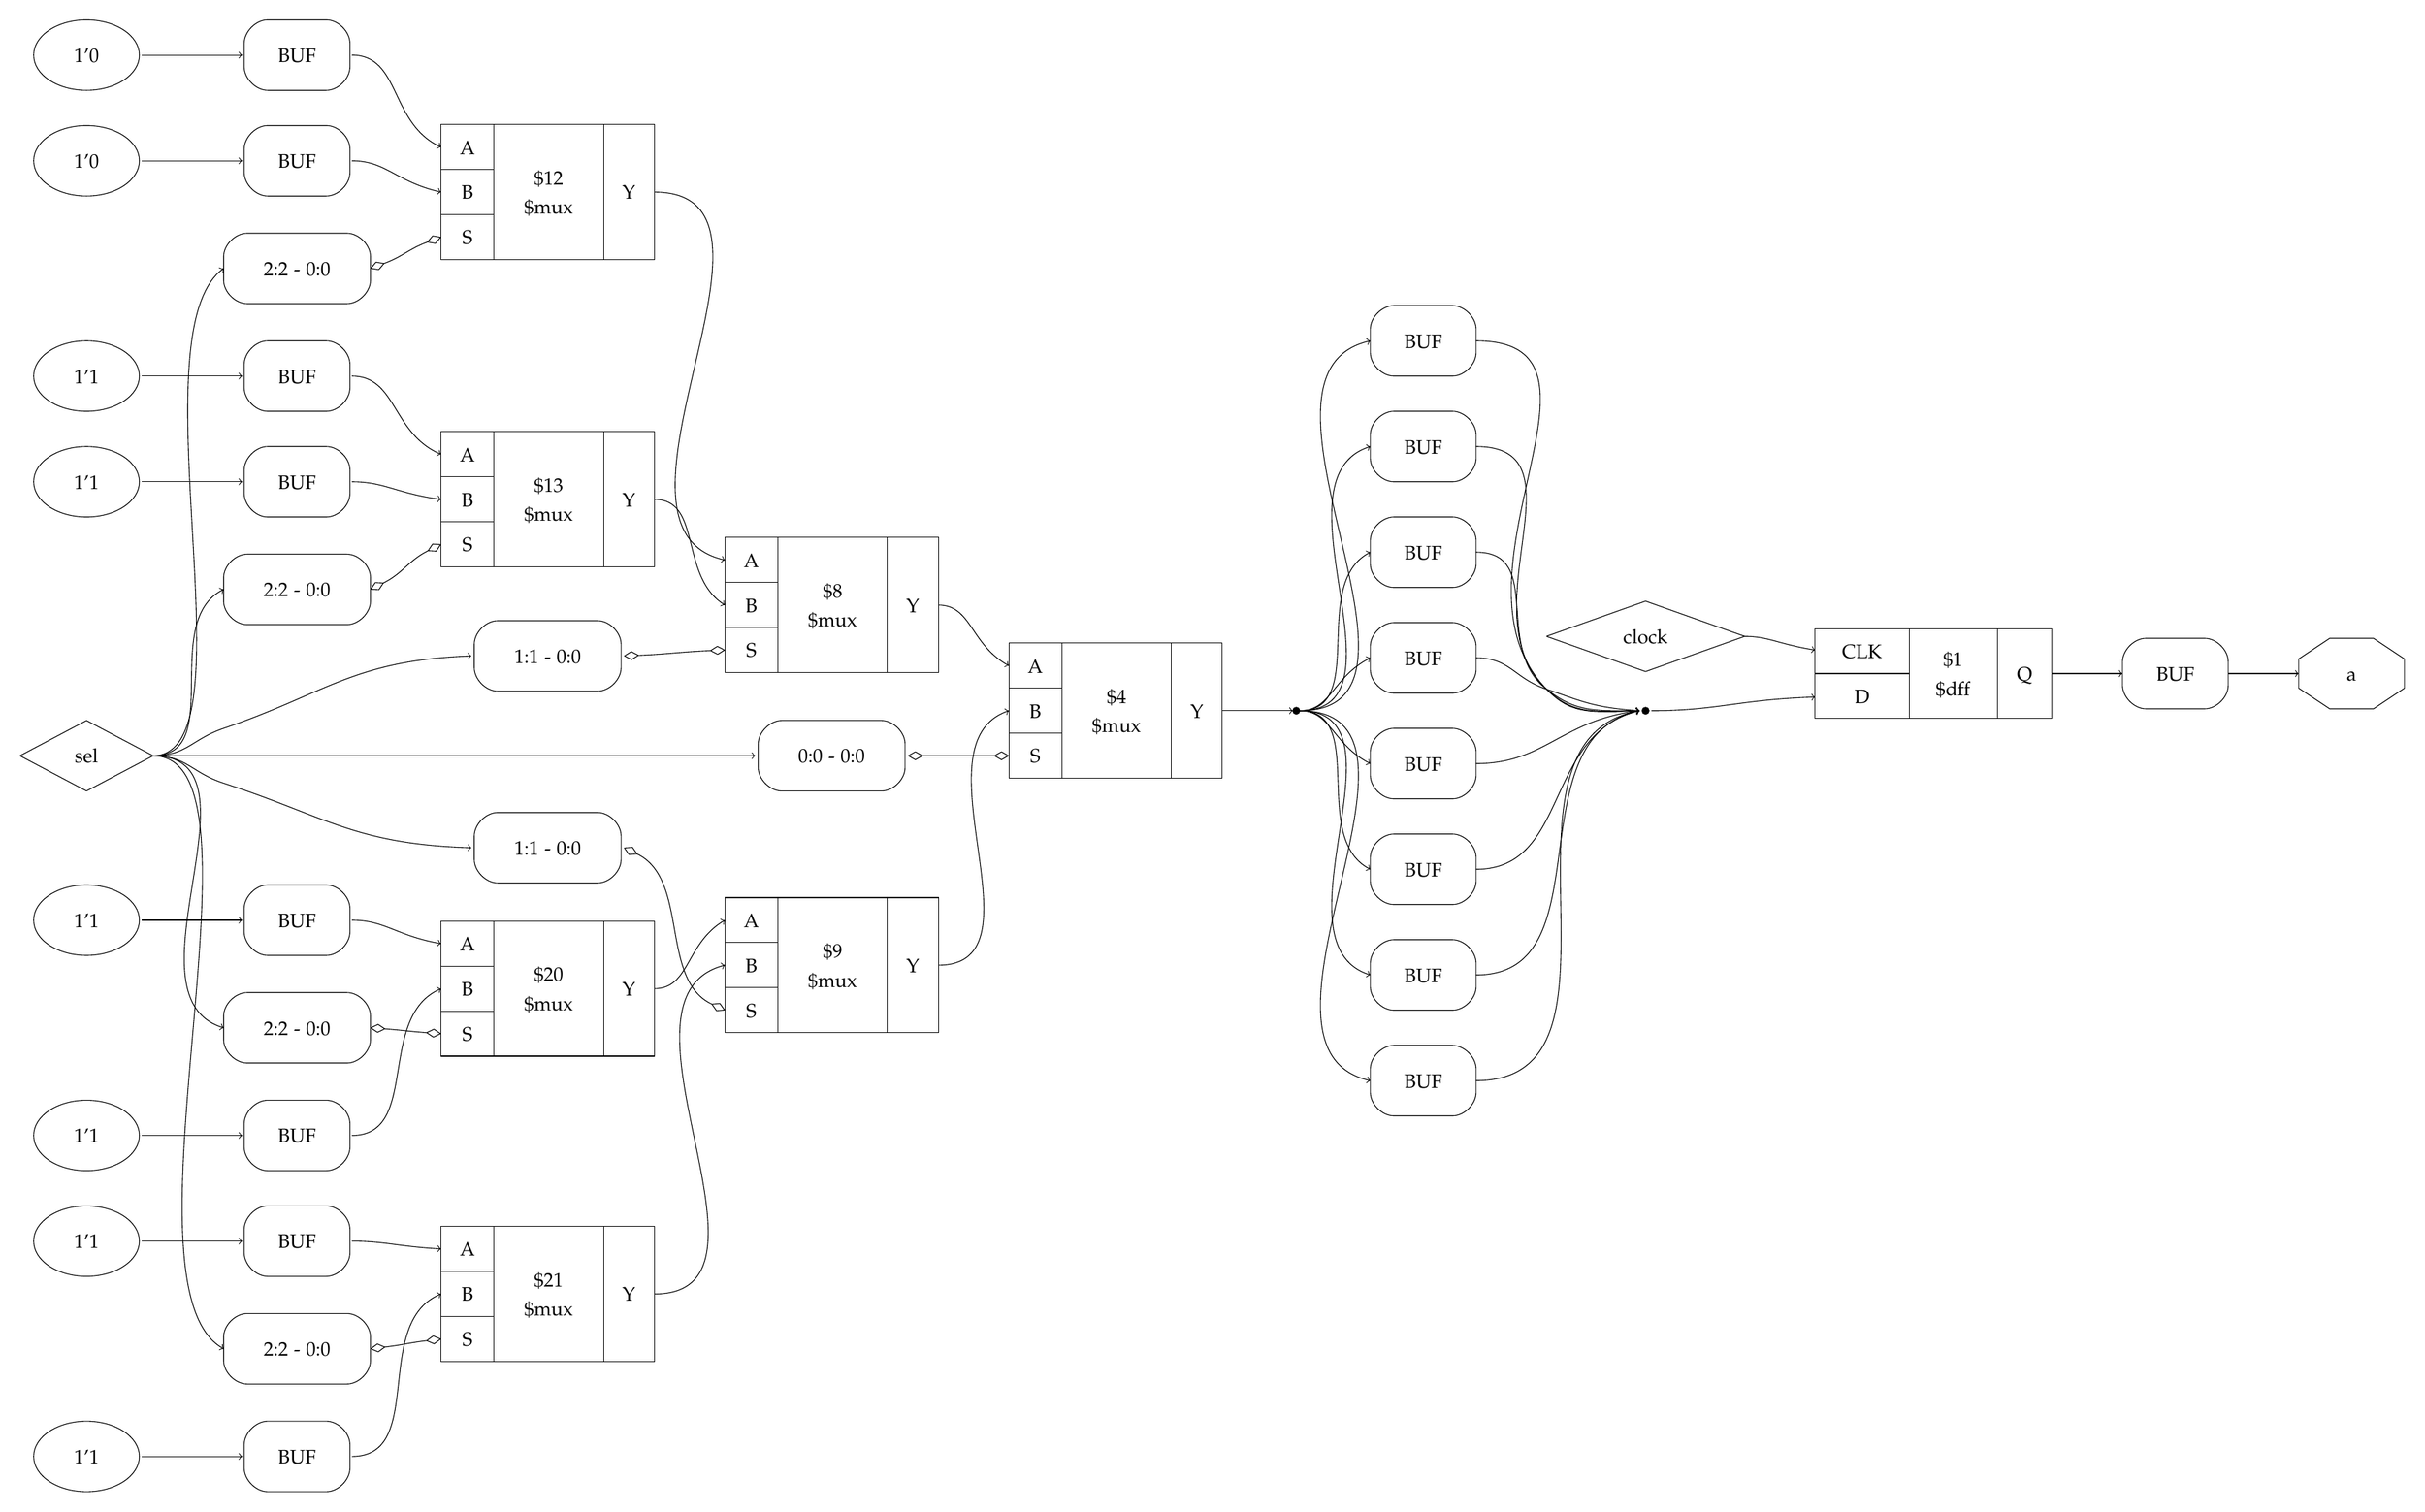
\begin{tikzpicture}[line join=bevel,anchor=base]%
\pgfsetcolor{black}
  % Edge: n19 -> x4
  \draw [->] (68.018bp,376.0bp) .. controls (85.185bp,376.0bp) and (87.685bp,367.29bp)  .. (104.02bp,362.0bp) .. controls (155.95bp,345.19bp) and (170.67bp,330.84bp)  .. (230.52bp,329.0bp);
  % Edge: n15 -> x28
  \draw [->] (653.62bp,399.0bp) .. controls (711.83bp,399.0bp) and (637.96bp,280.35bp)  .. (689.62bp,264.0bp);
  % Edge: x6 -> c31
  \draw [open diamond-open diamond] (453.52bp,376.0bp) .. controls (475.88bp,376.0bp) and (482.56bp,376.0bp)  .. (505.02bp,376.0bp);
  % Edge: x2 -> c27
  \draw [open diamond-open diamond] (179.02bp,461.0bp) .. controls (195.58bp,469.23bp) and (198.49bp,475.84bp)  .. (215.02bp,484.0bp);
  % Edge: v17 -> x18
  \draw [->] (62.009bp,128.0bp) .. controls (81.146bp,128.0bp) and (88.285bp,128.0bp)  .. (113.52bp,128.0bp);
  % Edge: v26 -> x27
  \draw [->] (62.009bp,516.0bp) .. controls (81.146bp,516.0bp) and (88.285bp,516.0bp)  .. (113.52bp,516.0bp);
  % Edge: n19 -> x0
  \draw [->] (68.018bp,376.0bp) .. controls (132.12bp,376.0bp) and (46.605bp,105.23bp)  .. (104.02bp,73.0bp);
  % Edge: x12 -> c26
  \draw [->] (169.52bp,292.0bp) .. controls (186.51bp,292.0bp) and (192.12bp,284.08bp)  .. (215.02bp,280.0bp);
  % Edge: n15 -> x19
  \draw [->] (653.62bp,399.0bp) .. controls (669.56bp,399.0bp) and (670.25bp,416.15bp)  .. (689.62bp,426.0bp);
  % Edge: x0 -> c25
  \draw [open diamond-open diamond] (179.02bp,73.0bp) .. controls (195.27bp,74.938bp) and (198.78bp,76.066bp)  .. (215.02bp,78.0bp);
  % Edge: n16 -> c35
  \draw [->] (833.17bp,399.0bp) .. controls (866.8bp,399.0bp) and (877.43bp,404.7bp)  .. (916.72bp,406.0bp);
  % Edge: c26 -> c29
  \draw [->] (324.02bp,257.0bp) .. controls (342.15bp,257.0bp) and (339.85bp,280.11bp)  .. (360.02bp,292.0bp);
  % Edge: v29 -> x30
  \draw [->] (62.009bp,18.0bp) .. controls (81.146bp,18.0bp) and (88.285bp,18.0bp)  .. (113.52bp,18.0bp);
  % Edge: x30 -> c25
  \draw [->] (169.52bp,18.0bp) .. controls (207.64bp,18.0bp) and (179.48bp,86.167bp)  .. (215.02bp,101.0bp);
  % Edge: n15 -> x31
  \draw [->] (653.62bp,399.0bp) .. controls (735.29bp,399.0bp) and (615.79bp,226.6bp)  .. (689.62bp,210.0bp);
  % Edge: v20 -> x21
  \draw [->] (62.009bp,680.0bp) .. controls (81.146bp,680.0bp) and (88.285bp,680.0bp)  .. (113.52bp,680.0bp);
  % Edge: x24 -> c26
  \draw [->] (169.52bp,182.0bp) .. controls (204.55bp,182.0bp) and (181.89bp,242.54bp)  .. (215.02bp,257.0bp);
  % Edge: n15 -> x9
  \draw [->] (653.62bp,399.0bp) .. controls (735.29bp,399.0bp) and (615.79bp,571.4bp)  .. (689.62bp,588.0bp);
  % Edge: x31 -> n16
  \draw [->] (743.62bp,210.0bp) .. controls (831.69bp,210.0bp) and (743.22bp,383.81bp)  .. (827.17bp,399.0bp);
  % Edge: v14 -> x15
  \draw [->] (62.009bp,570.0bp) .. controls (81.146bp,570.0bp) and (88.285bp,570.0bp)  .. (113.52bp,570.0bp);
  % Edge: v23 -> x24
  \draw [->] (62.009bp,182.0bp) .. controls (81.146bp,182.0bp) and (88.285bp,182.0bp)  .. (113.52bp,182.0bp);
  % Edge: x25 -> n16
  \draw [->] (743.62bp,318.0bp) .. controls (791.5bp,318.0bp) and (778.01bp,387.42bp)  .. (827.17bp,399.0bp);
  % Edge: v11 -> x12
  \draw [->] (62.009bp,292.0bp) .. controls (81.146bp,292.0bp) and (88.285bp,292.0bp)  .. (113.52bp,292.0bp);
  % Edge: x1 -> c26
  \draw [open diamond-open diamond] (179.02bp,237.0bp) .. controls (195.32bp,235.82bp) and (198.74bp,235.18bp)  .. (215.02bp,234.0bp);
  % Edge: n15 -> x22
  \draw [->] (653.62bp,399.0bp) .. controls (669.56bp,399.0bp) and (670.25bp,381.85bp)  .. (689.62bp,372.0bp);
  % Edge: x21 -> c28
  \draw [->] (169.52bp,680.0bp) .. controls (187.1bp,680.0bp) and (192.03bp,669.23bp)  .. (215.02bp,664.0bp);
  % Edge: x13 -> n16
  \draw [->] (743.62bp,534.0bp) .. controls (801.0bp,534.0bp) and (737.93bp,449.44bp)  .. (779.62bp,410.0bp) .. controls (792.67bp,397.65bp) and (801.84bp,398.21bp)  .. (827.17bp,399.0bp);
  % Edge: c28 -> c30
  \draw [->] (324.02bp,664.0bp) .. controls (405.27bp,664.0bp) and (286.55bp,492.51bp)  .. (360.02bp,476.0bp);
  % Edge: n19 -> x3
  \draw [->] (68.018bp,376.0bp) .. controls (120.0bp,376.0bp) and (58.12bp,591.22bp)  .. (104.02bp,625.0bp);
  % Edge: c27 -> c30
  \draw [->] (324.02bp,507.0bp) .. controls (348.58bp,507.0bp) and (336.5bp,467.84bp)  .. (360.02bp,453.0bp);
  % Edge: x19 -> n16
  \draw [->] (743.62bp,426.0bp) .. controls (761.13bp,426.0bp) and (763.01bp,415.55bp)  .. (779.62bp,410.0bp) .. controls (796.49bp,404.36bp) and (803.08bp,400.57bp)  .. (827.17bp,399.0bp);
  % Edge: x8 -> c28
  \draw [->] (169.52bp,734.0bp) .. controls (194.5bp,734.0bp) and (188.68bp,699.29bp)  .. (215.02bp,687.0bp);
  % Edge: x3 -> c28
  \draw [open diamond-open diamond] (179.02bp,625.0bp) .. controls (195.38bp,631.01bp) and (198.66bp,634.99bp)  .. (215.02bp,641.0bp);
  % Edge: c30 -> c31
  \draw [->] (469.02bp,453.0bp) .. controls (486.01bp,453.0bp) and (485.29bp,432.93bp)  .. (505.02bp,422.0bp);
  % Edge: c29 -> c31
  \draw [->] (469.02bp,269.0bp) .. controls (524.99bp,269.0bp) and (455.57bp,382.31bp)  .. (505.02bp,399.0bp);
  % Edge: x10 -> n20
  \draw [->] (1127.7bp,418.0bp) .. controls (1139.7bp,418.0bp) and (1145.0bp,418.0bp)  .. (1163.7bp,418.0bp);
  % Edge: n19 -> x6
  \draw [->] (68.018bp,376.0bp) .. controls (201.21bp,376.0bp) and (237.05bp,376.0bp)  .. (375.52bp,376.0bp);
  % Edge: x4 -> c29
  \draw [open diamond-open diamond] (308.52bp,329.0bp) .. controls (341.88bp,313.11bp) and (326.63bp,261.53bp)  .. (360.02bp,246.0bp);
  % Edge: c35 -> x10
  \draw [->] (1037.7bp,418.0bp) .. controls (1049.7bp,418.0bp) and (1055.0bp,418.0bp)  .. (1073.7bp,418.0bp);
  % Edge: n19 -> x2
  \draw [->] (68.018bp,376.0bp) .. controls (104.88bp,376.0bp) and (71.448bp,444.61bp)  .. (104.02bp,461.0bp);
  % Edge: c25 -> c29
  \draw [->] (324.02bp,101.0bp) .. controls (396.5bp,101.0bp) and (295.01bp,252.37bp)  .. (360.02bp,269.0bp);
  % Edge: x9 -> n16
  \draw [->] (743.62bp,588.0bp) .. controls (824.33bp,588.0bp) and (723.34bp,467.86bp)  .. (779.62bp,410.0bp) .. controls (792.14bp,397.12bp) and (801.66bp,398.03bp)  .. (827.17bp,399.0bp);
  % Edge: x18 -> c25
  \draw [->] (169.52bp,128.0bp) .. controls (186.01bp,128.0bp) and (192.34bp,125.36bp)  .. (215.02bp,124.0bp);
  % Edge: x5 -> c30
  \draw [open diamond-open diamond] (308.52bp,427.0bp) .. controls (330.89bp,427.9bp) and (337.55bp,429.09bp)  .. (360.02bp,430.0bp);
  % Edge: x22 -> n16
  \draw [->] (743.62bp,372.0bp) .. controls (778.98bp,372.0bp) and (786.82bp,394.17bp)  .. (827.17bp,399.0bp);
  % Edge: n19 -> x5
  \draw [->] (68.018bp,376.0bp) .. controls (85.185bp,376.0bp) and (87.764bp,384.47bp)  .. (104.02bp,390.0bp) .. controls (156.12bp,407.71bp) and (170.27bp,424.8bp)  .. (230.52bp,427.0bp);
  % Edge: x28 -> n16
  \draw [->] (743.62bp,264.0bp) .. controls (810.46bp,264.0bp) and (762.32bp,385.14bp)  .. (827.17bp,399.0bp);
  % Edge: n15 -> x16
  \draw [->] (653.62bp,399.0bp) .. controls (688.86bp,399.0bp) and (658.33bp,463.82bp)  .. (689.62bp,480.0bp);
  % Edge: x15 -> c27
  \draw [->] (169.52bp,570.0bp) .. controls (192.45bp,570.0bp) and (189.79bp,540.99bp)  .. (215.02bp,530.0bp);
  % Edge: n18 -> c35
  \draw [->] (880.72bp,437.0bp) .. controls (892.95bp,437.0bp) and (897.92bp,433.06bp)  .. (916.72bp,430.0bp);
  % Edge: x27 -> c27
  \draw [->] (169.52bp,516.0bp) .. controls (186.27bp,516.0bp) and (192.23bp,510.06bp)  .. (215.02bp,507.0bp);
  % Edge: n19 -> x1
  \draw [->] (68.018bp,376.0bp) .. controls (127.97bp,376.0bp) and (50.728bp,253.32bp)  .. (104.02bp,237.0bp);
  % Edge: n15 -> x13
  \draw [->] (653.62bp,399.0bp) .. controls (711.83bp,399.0bp) and (637.96bp,517.65bp)  .. (689.62bp,534.0bp);
  % Edge: x16 -> n16
  \draw [->] (743.62bp,480.0bp) .. controls (778.6bp,480.0bp) and (752.01bp,431.49bp)  .. (779.62bp,410.0bp) .. controls (793.79bp,398.96bp) and (802.23bp,398.66bp)  .. (827.17bp,399.0bp);
  % Edge: c31 -> n15
  \draw [->] (614.02bp,399.0bp) .. controls (626.02bp,399.0bp) and (631.27bp,399.0bp)  .. (650.02bp,399.0bp);
  % Edge: v7 -> x8
  \draw [->] (62.009bp,734.0bp) .. controls (81.146bp,734.0bp) and (88.285bp,734.0bp)  .. (113.52bp,734.0bp);
  % Edge: n15 -> x25
  \draw [->] (653.62bp,399.0bp) .. controls (688.86bp,399.0bp) and (658.33bp,334.18bp)  .. (689.62bp,318.0bp);
  % Node: n16
\begin{scope}
  \definecolor{strokecol}{rgb}{0.0,0.0,0.0};
  \pgfsetstrokecolor{strokecol}
  \definecolor{fillcol}{rgb}{0.0,0.0,0.0};
  \pgfsetfillcolor{fillcol}
  \filldraw [opacity=1] (830.17bp,399.0bp) ellipse (1.8bp and 1.8bp);
\end{scope}
  % Node: n15
\begin{scope}
  \definecolor{strokecol}{rgb}{0.0,0.0,0.0};
  \pgfsetstrokecolor{strokecol}
  \definecolor{fillcol}{rgb}{0.0,0.0,0.0};
  \pgfsetfillcolor{fillcol}
  \filldraw [opacity=1] (651.82bp,399.0bp) ellipse (1.8bp and 1.8bp);
\end{scope}
  % Node: n18
\begin{scope}
  \definecolor{strokecol}{rgb}{0.0,0.0,0.0};
  \pgfsetstrokecolor{strokecol}
  \draw (830.17bp,455.0bp) -- (779.56bp,437.0bp) -- (830.17bp,419.0bp) -- (880.78bp,437.0bp) -- cycle;
  \draw (830.17bp,433.3bp) node {clock};
\end{scope}
  % Node: n19
\begin{scope}
  \definecolor{strokecol}{rgb}{0.0,0.0,0.0};
  \pgfsetstrokecolor{strokecol}
  \draw (34.01bp,394.0bp) -- (-0.01bp,376.0bp) -- (34.01bp,358.0bp) -- (68.03bp,376.0bp) -- cycle;
  \draw (34.01bp,372.3bp) node {sel};
\end{scope}
  % Node: v17
\begin{scope}
  \definecolor{strokecol}{rgb}{0.0,0.0,0.0};
  \pgfsetstrokecolor{strokecol}
  \draw (34.01bp,128.0bp) ellipse (27.0bp and 18.0bp);
  \draw (34.01bp,124.3bp) node {1'1};
\end{scope}
  % Node: v14
\begin{scope}
  \definecolor{strokecol}{rgb}{0.0,0.0,0.0};
  \pgfsetstrokecolor{strokecol}
  \draw (34.01bp,570.0bp) ellipse (27.0bp and 18.0bp);
  \draw (34.01bp,566.3bp) node {1'1};
\end{scope}
  % Node: v20
\begin{scope}
  \definecolor{strokecol}{rgb}{0.0,0.0,0.0};
  \pgfsetstrokecolor{strokecol}
  \draw (34.01bp,680.0bp) ellipse (27.0bp and 18.0bp);
  \draw (34.01bp,676.3bp) node {1'0};
\end{scope}
  % Node: x1
\begin{scope}
  \definecolor{strokecol}{rgb}{0.0,0.0,0.0};
  \pgfsetstrokecolor{strokecol}
  \draw (116.02bp,219.0bp) .. controls (116.02bp,219.0bp) and (167.02bp,219.0bp)  .. (167.02bp,219.0bp) .. controls (173.02bp,219.0bp) and (179.02bp,225.0bp)  .. (179.02bp,231.0bp) .. controls (179.02bp,231.0bp) and (179.02bp,243.0bp)  .. (179.02bp,243.0bp) .. controls (179.02bp,249.0bp) and (173.02bp,255.0bp)  .. (167.02bp,255.0bp) .. controls (167.02bp,255.0bp) and (116.02bp,255.0bp)  .. (116.02bp,255.0bp) .. controls (110.02bp,255.0bp) and (104.02bp,249.0bp)  .. (104.02bp,243.0bp) .. controls (104.02bp,243.0bp) and (104.02bp,231.0bp)  .. (104.02bp,231.0bp) .. controls (104.02bp,225.0bp) and (110.02bp,219.0bp)  .. (116.02bp,219.0bp);
  \draw (141.52bp,233.3bp) node {2:2 - 0:0};
\end{scope}
  % Node: x28
\begin{scope}
  \definecolor{strokecol}{rgb}{0.0,0.0,0.0};
  \pgfsetstrokecolor{strokecol}
  \draw (731.62bp,282.0bp) .. controls (731.62bp,282.0bp) and (701.62bp,282.0bp)  .. (701.62bp,282.0bp) .. controls (695.62bp,282.0bp) and (689.62bp,276.0bp)  .. (689.62bp,270.0bp) .. controls (689.62bp,270.0bp) and (689.62bp,258.0bp)  .. (689.62bp,258.0bp) .. controls (689.62bp,252.0bp) and (695.62bp,246.0bp)  .. (701.62bp,246.0bp) .. controls (701.62bp,246.0bp) and (731.62bp,246.0bp)  .. (731.62bp,246.0bp) .. controls (737.62bp,246.0bp) and (743.62bp,252.0bp)  .. (743.62bp,258.0bp) .. controls (743.62bp,258.0bp) and (743.62bp,270.0bp)  .. (743.62bp,270.0bp) .. controls (743.62bp,276.0bp) and (737.62bp,282.0bp)  .. (731.62bp,282.0bp);
  \draw (716.62bp,260.3bp) node {BUF};
\end{scope}
  % Node: c35
\begin{scope}
  \definecolor{strokecol}{rgb}{0.0,0.0,0.0};
  \pgfsetstrokecolor{strokecol}
  \draw (916.72bp,395.0bp) -- (916.72bp,441.0bp) -- (1037.72bp,441.0bp) -- (1037.72bp,395.0bp) -- cycle;
  \draw (916.72bp,418.0bp) -- (964.72bp,418.0bp);
  \draw (964.72bp,395.0bp) -- (964.72bp,441.0bp);
  \draw (1009.72bp,395.0bp) -- (1009.72bp,441.0bp);
  \draw (940.72bp,425.8bp) node {CLK};
  \draw (940.72bp,402.8bp) node {D};
  \draw (987.22bp,421.8bp) node {\$1};
  \draw (987.22bp,406.8bp) node {\$dff};
  \draw (1023.72bp,414.3bp) node {Q};
\end{scope}
  % Node: x24
\begin{scope}
  \definecolor{strokecol}{rgb}{0.0,0.0,0.0};
  \pgfsetstrokecolor{strokecol}
  \draw (156.52bp,200.0bp) .. controls (156.52bp,200.0bp) and (126.52bp,200.0bp)  .. (126.52bp,200.0bp) .. controls (120.52bp,200.0bp) and (114.52bp,194.0bp)  .. (114.52bp,188.0bp) .. controls (114.52bp,188.0bp) and (114.52bp,176.0bp)  .. (114.52bp,176.0bp) .. controls (114.52bp,170.0bp) and (120.52bp,164.0bp)  .. (126.52bp,164.0bp) .. controls (126.52bp,164.0bp) and (156.52bp,164.0bp)  .. (156.52bp,164.0bp) .. controls (162.52bp,164.0bp) and (168.52bp,170.0bp)  .. (168.52bp,176.0bp) .. controls (168.52bp,176.0bp) and (168.52bp,188.0bp)  .. (168.52bp,188.0bp) .. controls (168.52bp,194.0bp) and (162.52bp,200.0bp)  .. (156.52bp,200.0bp);
  \draw (141.52bp,178.3bp) node {BUF};
\end{scope}
  % Node: x27
\begin{scope}
  \definecolor{strokecol}{rgb}{0.0,0.0,0.0};
  \pgfsetstrokecolor{strokecol}
  \draw (156.52bp,534.0bp) .. controls (156.52bp,534.0bp) and (126.52bp,534.0bp)  .. (126.52bp,534.0bp) .. controls (120.52bp,534.0bp) and (114.52bp,528.0bp)  .. (114.52bp,522.0bp) .. controls (114.52bp,522.0bp) and (114.52bp,510.0bp)  .. (114.52bp,510.0bp) .. controls (114.52bp,504.0bp) and (120.52bp,498.0bp)  .. (126.52bp,498.0bp) .. controls (126.52bp,498.0bp) and (156.52bp,498.0bp)  .. (156.52bp,498.0bp) .. controls (162.52bp,498.0bp) and (168.52bp,504.0bp)  .. (168.52bp,510.0bp) .. controls (168.52bp,510.0bp) and (168.52bp,522.0bp)  .. (168.52bp,522.0bp) .. controls (168.52bp,528.0bp) and (162.52bp,534.0bp)  .. (156.52bp,534.0bp);
  \draw (141.52bp,512.3bp) node {BUF};
\end{scope}
  % Node: c31
\begin{scope}
  \definecolor{strokecol}{rgb}{0.0,0.0,0.0};
  \pgfsetstrokecolor{strokecol}
  \draw (505.02bp,364.5bp) -- (505.02bp,433.5bp) -- (614.02bp,433.5bp) -- (614.02bp,364.5bp) -- cycle;
  \draw (505.02bp,410.5bp) -- (532.02bp,410.5bp);
  \draw (505.02bp,387.5bp) -- (532.02bp,387.5bp);
  \draw (532.02bp,364.5bp) -- (532.02bp,433.5bp);
  \draw (588.02bp,364.5bp) -- (588.02bp,433.5bp);
  \draw (518.52bp,418.3bp) node {A};
  \draw (518.52bp,395.3bp) node {B};
  \draw (518.52bp,372.3bp) node {S};
  \draw (560.02bp,402.8bp) node {\$4};
  \draw (560.02bp,387.8bp) node {\$mux};
  \draw (601.02bp,395.3bp) node {Y};
\end{scope}
  % Node: c30
\begin{scope}
  \definecolor{strokecol}{rgb}{0.0,0.0,0.0};
  \pgfsetstrokecolor{strokecol}
  \draw (360.02bp,418.5bp) -- (360.02bp,487.5bp) -- (469.02bp,487.5bp) -- (469.02bp,418.5bp) -- cycle;
  \draw (360.02bp,464.5bp) -- (387.02bp,464.5bp);
  \draw (360.02bp,441.5bp) -- (387.02bp,441.5bp);
  \draw (387.02bp,418.5bp) -- (387.02bp,487.5bp);
  \draw (443.02bp,418.5bp) -- (443.02bp,487.5bp);
  \draw (373.52bp,472.3bp) node {A};
  \draw (373.52bp,449.3bp) node {B};
  \draw (373.52bp,426.3bp) node {S};
  \draw (415.02bp,456.8bp) node {\$8};
  \draw (415.02bp,441.8bp) node {\$mux};
  \draw (456.02bp,449.3bp) node {Y};
\end{scope}
  % Node: x22
\begin{scope}
  \definecolor{strokecol}{rgb}{0.0,0.0,0.0};
  \pgfsetstrokecolor{strokecol}
  \draw (731.62bp,390.0bp) .. controls (731.62bp,390.0bp) and (701.62bp,390.0bp)  .. (701.62bp,390.0bp) .. controls (695.62bp,390.0bp) and (689.62bp,384.0bp)  .. (689.62bp,378.0bp) .. controls (689.62bp,378.0bp) and (689.62bp,366.0bp)  .. (689.62bp,366.0bp) .. controls (689.62bp,360.0bp) and (695.62bp,354.0bp)  .. (701.62bp,354.0bp) .. controls (701.62bp,354.0bp) and (731.62bp,354.0bp)  .. (731.62bp,354.0bp) .. controls (737.62bp,354.0bp) and (743.62bp,360.0bp)  .. (743.62bp,366.0bp) .. controls (743.62bp,366.0bp) and (743.62bp,378.0bp)  .. (743.62bp,378.0bp) .. controls (743.62bp,384.0bp) and (737.62bp,390.0bp)  .. (731.62bp,390.0bp);
  \draw (716.62bp,368.3bp) node {BUF};
\end{scope}
  % Node: v23
\begin{scope}
  \definecolor{strokecol}{rgb}{0.0,0.0,0.0};
  \pgfsetstrokecolor{strokecol}
  \draw (34.01bp,182.0bp) ellipse (27.0bp and 18.0bp);
  \draw (34.01bp,178.3bp) node {1'1};
\end{scope}
  % Node: v11
\begin{scope}
  \definecolor{strokecol}{rgb}{0.0,0.0,0.0};
  \pgfsetstrokecolor{strokecol}
  \draw (34.01bp,292.0bp) ellipse (27.0bp and 18.0bp);
  \draw (34.01bp,288.3bp) node {1'1};
\end{scope}
  % Node: v26
\begin{scope}
  \definecolor{strokecol}{rgb}{0.0,0.0,0.0};
  \pgfsetstrokecolor{strokecol}
  \draw (34.01bp,516.0bp) ellipse (27.0bp and 18.0bp);
  \draw (34.01bp,512.3bp) node {1'1};
\end{scope}
  % Node: v29
\begin{scope}
  \definecolor{strokecol}{rgb}{0.0,0.0,0.0};
  \pgfsetstrokecolor{strokecol}
  \draw (34.01bp,18.0bp) ellipse (27.0bp and 18.0bp);
  \draw (34.01bp,14.3bp) node {1'1};
\end{scope}
  % Node: x25
\begin{scope}
  \definecolor{strokecol}{rgb}{0.0,0.0,0.0};
  \pgfsetstrokecolor{strokecol}
  \draw (731.62bp,336.0bp) .. controls (731.62bp,336.0bp) and (701.62bp,336.0bp)  .. (701.62bp,336.0bp) .. controls (695.62bp,336.0bp) and (689.62bp,330.0bp)  .. (689.62bp,324.0bp) .. controls (689.62bp,324.0bp) and (689.62bp,312.0bp)  .. (689.62bp,312.0bp) .. controls (689.62bp,306.0bp) and (695.62bp,300.0bp)  .. (701.62bp,300.0bp) .. controls (701.62bp,300.0bp) and (731.62bp,300.0bp)  .. (731.62bp,300.0bp) .. controls (737.62bp,300.0bp) and (743.62bp,306.0bp)  .. (743.62bp,312.0bp) .. controls (743.62bp,312.0bp) and (743.62bp,324.0bp)  .. (743.62bp,324.0bp) .. controls (743.62bp,330.0bp) and (737.62bp,336.0bp)  .. (731.62bp,336.0bp);
  \draw (716.62bp,314.3bp) node {BUF};
\end{scope}
  % Node: x8
\begin{scope}
  \definecolor{strokecol}{rgb}{0.0,0.0,0.0};
  \pgfsetstrokecolor{strokecol}
  \draw (156.52bp,752.0bp) .. controls (156.52bp,752.0bp) and (126.52bp,752.0bp)  .. (126.52bp,752.0bp) .. controls (120.52bp,752.0bp) and (114.52bp,746.0bp)  .. (114.52bp,740.0bp) .. controls (114.52bp,740.0bp) and (114.52bp,728.0bp)  .. (114.52bp,728.0bp) .. controls (114.52bp,722.0bp) and (120.52bp,716.0bp)  .. (126.52bp,716.0bp) .. controls (126.52bp,716.0bp) and (156.52bp,716.0bp)  .. (156.52bp,716.0bp) .. controls (162.52bp,716.0bp) and (168.52bp,722.0bp)  .. (168.52bp,728.0bp) .. controls (168.52bp,728.0bp) and (168.52bp,740.0bp)  .. (168.52bp,740.0bp) .. controls (168.52bp,746.0bp) and (162.52bp,752.0bp)  .. (156.52bp,752.0bp);
  \draw (141.52bp,730.3bp) node {BUF};
\end{scope}
  % Node: x9
\begin{scope}
  \definecolor{strokecol}{rgb}{0.0,0.0,0.0};
  \pgfsetstrokecolor{strokecol}
  \draw (731.62bp,606.0bp) .. controls (731.62bp,606.0bp) and (701.62bp,606.0bp)  .. (701.62bp,606.0bp) .. controls (695.62bp,606.0bp) and (689.62bp,600.0bp)  .. (689.62bp,594.0bp) .. controls (689.62bp,594.0bp) and (689.62bp,582.0bp)  .. (689.62bp,582.0bp) .. controls (689.62bp,576.0bp) and (695.62bp,570.0bp)  .. (701.62bp,570.0bp) .. controls (701.62bp,570.0bp) and (731.62bp,570.0bp)  .. (731.62bp,570.0bp) .. controls (737.62bp,570.0bp) and (743.62bp,576.0bp)  .. (743.62bp,582.0bp) .. controls (743.62bp,582.0bp) and (743.62bp,594.0bp)  .. (743.62bp,594.0bp) .. controls (743.62bp,600.0bp) and (737.62bp,606.0bp)  .. (731.62bp,606.0bp);
  \draw (716.62bp,584.3bp) node {BUF};
\end{scope}
  % Node: v7
\begin{scope}
  \definecolor{strokecol}{rgb}{0.0,0.0,0.0};
  \pgfsetstrokecolor{strokecol}
  \draw (34.01bp,734.0bp) ellipse (27.0bp and 18.0bp);
  \draw (34.01bp,730.3bp) node {1'0};
\end{scope}
  % Node: x2
\begin{scope}
  \definecolor{strokecol}{rgb}{0.0,0.0,0.0};
  \pgfsetstrokecolor{strokecol}
  \draw (116.02bp,443.0bp) .. controls (116.02bp,443.0bp) and (167.02bp,443.0bp)  .. (167.02bp,443.0bp) .. controls (173.02bp,443.0bp) and (179.02bp,449.0bp)  .. (179.02bp,455.0bp) .. controls (179.02bp,455.0bp) and (179.02bp,467.0bp)  .. (179.02bp,467.0bp) .. controls (179.02bp,473.0bp) and (173.02bp,479.0bp)  .. (167.02bp,479.0bp) .. controls (167.02bp,479.0bp) and (116.02bp,479.0bp)  .. (116.02bp,479.0bp) .. controls (110.02bp,479.0bp) and (104.02bp,473.0bp)  .. (104.02bp,467.0bp) .. controls (104.02bp,467.0bp) and (104.02bp,455.0bp)  .. (104.02bp,455.0bp) .. controls (104.02bp,449.0bp) and (110.02bp,443.0bp)  .. (116.02bp,443.0bp);
  \draw (141.52bp,457.3bp) node {2:2 - 0:0};
\end{scope}
  % Node: x3
\begin{scope}
  \definecolor{strokecol}{rgb}{0.0,0.0,0.0};
  \pgfsetstrokecolor{strokecol}
  \draw (116.02bp,607.0bp) .. controls (116.02bp,607.0bp) and (167.02bp,607.0bp)  .. (167.02bp,607.0bp) .. controls (173.02bp,607.0bp) and (179.02bp,613.0bp)  .. (179.02bp,619.0bp) .. controls (179.02bp,619.0bp) and (179.02bp,631.0bp)  .. (179.02bp,631.0bp) .. controls (179.02bp,637.0bp) and (173.02bp,643.0bp)  .. (167.02bp,643.0bp) .. controls (167.02bp,643.0bp) and (116.02bp,643.0bp)  .. (116.02bp,643.0bp) .. controls (110.02bp,643.0bp) and (104.02bp,637.0bp)  .. (104.02bp,631.0bp) .. controls (104.02bp,631.0bp) and (104.02bp,619.0bp)  .. (104.02bp,619.0bp) .. controls (104.02bp,613.0bp) and (110.02bp,607.0bp)  .. (116.02bp,607.0bp);
  \draw (141.52bp,621.3bp) node {2:2 - 0:0};
\end{scope}
  % Node: x0
\begin{scope}
  \definecolor{strokecol}{rgb}{0.0,0.0,0.0};
  \pgfsetstrokecolor{strokecol}
  \draw (116.02bp,55.0bp) .. controls (116.02bp,55.0bp) and (167.02bp,55.0bp)  .. (167.02bp,55.0bp) .. controls (173.02bp,55.0bp) and (179.02bp,61.0bp)  .. (179.02bp,67.0bp) .. controls (179.02bp,67.0bp) and (179.02bp,79.0bp)  .. (179.02bp,79.0bp) .. controls (179.02bp,85.0bp) and (173.02bp,91.0bp)  .. (167.02bp,91.0bp) .. controls (167.02bp,91.0bp) and (116.02bp,91.0bp)  .. (116.02bp,91.0bp) .. controls (110.02bp,91.0bp) and (104.02bp,85.0bp)  .. (104.02bp,79.0bp) .. controls (104.02bp,79.0bp) and (104.02bp,67.0bp)  .. (104.02bp,67.0bp) .. controls (104.02bp,61.0bp) and (110.02bp,55.0bp)  .. (116.02bp,55.0bp);
  \draw (141.52bp,69.3bp) node {2:2 - 0:0};
\end{scope}
  % Node: n20
\begin{scope}
  \definecolor{strokecol}{rgb}{0.0,0.0,0.0};
  \pgfsetstrokecolor{strokecol}
  \draw (1217.72bp,410.54bp) -- (1217.72bp,425.46bp) -- (1201.91bp,436.0bp) -- (1179.54bp,436.0bp) -- (1163.72bp,425.46bp) -- (1163.72bp,410.54bp) -- (1179.54bp,400.0bp) -- (1201.91bp,400.0bp) -- cycle;
  \draw (1190.72bp,414.3bp) node {a};
\end{scope}
  % Node: x6
\begin{scope}
  \definecolor{strokecol}{rgb}{0.0,0.0,0.0};
  \pgfsetstrokecolor{strokecol}
  \draw (389.02bp,358.0bp) .. controls (389.02bp,358.0bp) and (440.02bp,358.0bp)  .. (440.02bp,358.0bp) .. controls (446.02bp,358.0bp) and (452.02bp,364.0bp)  .. (452.02bp,370.0bp) .. controls (452.02bp,370.0bp) and (452.02bp,382.0bp)  .. (452.02bp,382.0bp) .. controls (452.02bp,388.0bp) and (446.02bp,394.0bp)  .. (440.02bp,394.0bp) .. controls (440.02bp,394.0bp) and (389.02bp,394.0bp)  .. (389.02bp,394.0bp) .. controls (383.02bp,394.0bp) and (377.02bp,388.0bp)  .. (377.02bp,382.0bp) .. controls (377.02bp,382.0bp) and (377.02bp,370.0bp)  .. (377.02bp,370.0bp) .. controls (377.02bp,364.0bp) and (383.02bp,358.0bp)  .. (389.02bp,358.0bp);
  \draw (414.52bp,372.3bp) node {0:0 - 0:0};
\end{scope}
  % Node: x4
\begin{scope}
  \definecolor{strokecol}{rgb}{0.0,0.0,0.0};
  \pgfsetstrokecolor{strokecol}
  \draw (244.02bp,311.0bp) .. controls (244.02bp,311.0bp) and (295.02bp,311.0bp)  .. (295.02bp,311.0bp) .. controls (301.02bp,311.0bp) and (307.02bp,317.0bp)  .. (307.02bp,323.0bp) .. controls (307.02bp,323.0bp) and (307.02bp,335.0bp)  .. (307.02bp,335.0bp) .. controls (307.02bp,341.0bp) and (301.02bp,347.0bp)  .. (295.02bp,347.0bp) .. controls (295.02bp,347.0bp) and (244.02bp,347.0bp)  .. (244.02bp,347.0bp) .. controls (238.02bp,347.0bp) and (232.02bp,341.0bp)  .. (232.02bp,335.0bp) .. controls (232.02bp,335.0bp) and (232.02bp,323.0bp)  .. (232.02bp,323.0bp) .. controls (232.02bp,317.0bp) and (238.02bp,311.0bp)  .. (244.02bp,311.0bp);
  \draw (269.52bp,325.3bp) node {1:1 - 0:0};
\end{scope}
  % Node: x5
\begin{scope}
  \definecolor{strokecol}{rgb}{0.0,0.0,0.0};
  \pgfsetstrokecolor{strokecol}
  \draw (244.02bp,409.0bp) .. controls (244.02bp,409.0bp) and (295.02bp,409.0bp)  .. (295.02bp,409.0bp) .. controls (301.02bp,409.0bp) and (307.02bp,415.0bp)  .. (307.02bp,421.0bp) .. controls (307.02bp,421.0bp) and (307.02bp,433.0bp)  .. (307.02bp,433.0bp) .. controls (307.02bp,439.0bp) and (301.02bp,445.0bp)  .. (295.02bp,445.0bp) .. controls (295.02bp,445.0bp) and (244.02bp,445.0bp)  .. (244.02bp,445.0bp) .. controls (238.02bp,445.0bp) and (232.02bp,439.0bp)  .. (232.02bp,433.0bp) .. controls (232.02bp,433.0bp) and (232.02bp,421.0bp)  .. (232.02bp,421.0bp) .. controls (232.02bp,415.0bp) and (238.02bp,409.0bp)  .. (244.02bp,409.0bp);
  \draw (269.52bp,423.3bp) node {1:1 - 0:0};
\end{scope}
  % Node: x30
\begin{scope}
  \definecolor{strokecol}{rgb}{0.0,0.0,0.0};
  \pgfsetstrokecolor{strokecol}
  \draw (156.52bp,36.0bp) .. controls (156.52bp,36.0bp) and (126.52bp,36.0bp)  .. (126.52bp,36.0bp) .. controls (120.52bp,36.0bp) and (114.52bp,30.0bp)  .. (114.52bp,24.0bp) .. controls (114.52bp,24.0bp) and (114.52bp,12.0bp)  .. (114.52bp,12.0bp) .. controls (114.52bp,6.0bp) and (120.52bp,0.0bp)  .. (126.52bp,0.0bp) .. controls (126.52bp,0.0bp) and (156.52bp,0.0bp)  .. (156.52bp,0.0bp) .. controls (162.52bp,0.0bp) and (168.52bp,6.0bp)  .. (168.52bp,12.0bp) .. controls (168.52bp,12.0bp) and (168.52bp,24.0bp)  .. (168.52bp,24.0bp) .. controls (168.52bp,30.0bp) and (162.52bp,36.0bp)  .. (156.52bp,36.0bp);
  \draw (141.52bp,14.3bp) node {BUF};
\end{scope}
  % Node: x31
\begin{scope}
  \definecolor{strokecol}{rgb}{0.0,0.0,0.0};
  \pgfsetstrokecolor{strokecol}
  \draw (731.62bp,228.0bp) .. controls (731.62bp,228.0bp) and (701.62bp,228.0bp)  .. (701.62bp,228.0bp) .. controls (695.62bp,228.0bp) and (689.62bp,222.0bp)  .. (689.62bp,216.0bp) .. controls (689.62bp,216.0bp) and (689.62bp,204.0bp)  .. (689.62bp,204.0bp) .. controls (689.62bp,198.0bp) and (695.62bp,192.0bp)  .. (701.62bp,192.0bp) .. controls (701.62bp,192.0bp) and (731.62bp,192.0bp)  .. (731.62bp,192.0bp) .. controls (737.62bp,192.0bp) and (743.62bp,198.0bp)  .. (743.62bp,204.0bp) .. controls (743.62bp,204.0bp) and (743.62bp,216.0bp)  .. (743.62bp,216.0bp) .. controls (743.62bp,222.0bp) and (737.62bp,228.0bp)  .. (731.62bp,228.0bp);
  \draw (716.62bp,206.3bp) node {BUF};
\end{scope}
  % Node: c26
\begin{scope}
  \definecolor{strokecol}{rgb}{0.0,0.0,0.0};
  \pgfsetstrokecolor{strokecol}
  \draw (215.02bp,222.5bp) -- (215.02bp,291.5bp) -- (324.02bp,291.5bp) -- (324.02bp,222.5bp) -- cycle;
  \draw (215.02bp,268.5bp) -- (242.02bp,268.5bp);
  \draw (215.02bp,245.5bp) -- (242.02bp,245.5bp);
  \draw (242.02bp,222.5bp) -- (242.02bp,291.5bp);
  \draw (298.02bp,222.5bp) -- (298.02bp,291.5bp);
  \draw (228.52bp,276.3bp) node {A};
  \draw (228.52bp,253.3bp) node {B};
  \draw (228.52bp,230.3bp) node {S};
  \draw (270.02bp,260.8bp) node {\$20};
  \draw (270.02bp,245.8bp) node {\$mux};
  \draw (311.02bp,253.3bp) node {Y};
\end{scope}
  % Node: c27
\begin{scope}
  \definecolor{strokecol}{rgb}{0.0,0.0,0.0};
  \pgfsetstrokecolor{strokecol}
  \draw (215.02bp,472.5bp) -- (215.02bp,541.5bp) -- (324.02bp,541.5bp) -- (324.02bp,472.5bp) -- cycle;
  \draw (215.02bp,518.5bp) -- (242.02bp,518.5bp);
  \draw (215.02bp,495.5bp) -- (242.02bp,495.5bp);
  \draw (242.02bp,472.5bp) -- (242.02bp,541.5bp);
  \draw (298.02bp,472.5bp) -- (298.02bp,541.5bp);
  \draw (228.52bp,526.3bp) node {A};
  \draw (228.52bp,503.3bp) node {B};
  \draw (228.52bp,480.3bp) node {S};
  \draw (270.02bp,510.8bp) node {\$13};
  \draw (270.02bp,495.8bp) node {\$mux};
  \draw (311.02bp,503.3bp) node {Y};
\end{scope}
  % Node: c25
\begin{scope}
  \definecolor{strokecol}{rgb}{0.0,0.0,0.0};
  \pgfsetstrokecolor{strokecol}
  \draw (215.02bp,66.5bp) -- (215.02bp,135.5bp) -- (324.02bp,135.5bp) -- (324.02bp,66.5bp) -- cycle;
  \draw (215.02bp,112.5bp) -- (242.02bp,112.5bp);
  \draw (215.02bp,89.5bp) -- (242.02bp,89.5bp);
  \draw (242.02bp,66.5bp) -- (242.02bp,135.5bp);
  \draw (298.02bp,66.5bp) -- (298.02bp,135.5bp);
  \draw (228.52bp,120.3bp) node {A};
  \draw (228.52bp,97.3bp) node {B};
  \draw (228.52bp,74.3bp) node {S};
  \draw (270.02bp,104.8bp) node {\$21};
  \draw (270.02bp,89.8bp) node {\$mux};
  \draw (311.02bp,97.3bp) node {Y};
\end{scope}
  % Node: x21
\begin{scope}
  \definecolor{strokecol}{rgb}{0.0,0.0,0.0};
  \pgfsetstrokecolor{strokecol}
  \draw (156.52bp,698.0bp) .. controls (156.52bp,698.0bp) and (126.52bp,698.0bp)  .. (126.52bp,698.0bp) .. controls (120.52bp,698.0bp) and (114.52bp,692.0bp)  .. (114.52bp,686.0bp) .. controls (114.52bp,686.0bp) and (114.52bp,674.0bp)  .. (114.52bp,674.0bp) .. controls (114.52bp,668.0bp) and (120.52bp,662.0bp)  .. (126.52bp,662.0bp) .. controls (126.52bp,662.0bp) and (156.52bp,662.0bp)  .. (156.52bp,662.0bp) .. controls (162.52bp,662.0bp) and (168.52bp,668.0bp)  .. (168.52bp,674.0bp) .. controls (168.52bp,674.0bp) and (168.52bp,686.0bp)  .. (168.52bp,686.0bp) .. controls (168.52bp,692.0bp) and (162.52bp,698.0bp)  .. (156.52bp,698.0bp);
  \draw (141.52bp,676.3bp) node {BUF};
\end{scope}
  % Node: c28
\begin{scope}
  \definecolor{strokecol}{rgb}{0.0,0.0,0.0};
  \pgfsetstrokecolor{strokecol}
  \draw (215.02bp,629.5bp) -- (215.02bp,698.5bp) -- (324.02bp,698.5bp) -- (324.02bp,629.5bp) -- cycle;
  \draw (215.02bp,675.5bp) -- (242.02bp,675.5bp);
  \draw (215.02bp,652.5bp) -- (242.02bp,652.5bp);
  \draw (242.02bp,629.5bp) -- (242.02bp,698.5bp);
  \draw (298.02bp,629.5bp) -- (298.02bp,698.5bp);
  \draw (228.52bp,683.3bp) node {A};
  \draw (228.52bp,660.3bp) node {B};
  \draw (228.52bp,637.3bp) node {S};
  \draw (270.02bp,667.8bp) node {\$12};
  \draw (270.02bp,652.8bp) node {\$mux};
  \draw (311.02bp,660.3bp) node {Y};
\end{scope}
  % Node: c29
\begin{scope}
  \definecolor{strokecol}{rgb}{0.0,0.0,0.0};
  \pgfsetstrokecolor{strokecol}
  \draw (360.02bp,234.5bp) -- (360.02bp,303.5bp) -- (469.02bp,303.5bp) -- (469.02bp,234.5bp) -- cycle;
  \draw (360.02bp,280.5bp) -- (387.02bp,280.5bp);
  \draw (360.02bp,257.5bp) -- (387.02bp,257.5bp);
  \draw (387.02bp,234.5bp) -- (387.02bp,303.5bp);
  \draw (443.02bp,234.5bp) -- (443.02bp,303.5bp);
  \draw (373.52bp,288.3bp) node {A};
  \draw (373.52bp,265.3bp) node {B};
  \draw (373.52bp,242.3bp) node {S};
  \draw (415.02bp,272.8bp) node {\$9};
  \draw (415.02bp,257.8bp) node {\$mux};
  \draw (456.02bp,265.3bp) node {Y};
\end{scope}
  % Node: x18
\begin{scope}
  \definecolor{strokecol}{rgb}{0.0,0.0,0.0};
  \pgfsetstrokecolor{strokecol}
  \draw (156.52bp,146.0bp) .. controls (156.52bp,146.0bp) and (126.52bp,146.0bp)  .. (126.52bp,146.0bp) .. controls (120.52bp,146.0bp) and (114.52bp,140.0bp)  .. (114.52bp,134.0bp) .. controls (114.52bp,134.0bp) and (114.52bp,122.0bp)  .. (114.52bp,122.0bp) .. controls (114.52bp,116.0bp) and (120.52bp,110.0bp)  .. (126.52bp,110.0bp) .. controls (126.52bp,110.0bp) and (156.52bp,110.0bp)  .. (156.52bp,110.0bp) .. controls (162.52bp,110.0bp) and (168.52bp,116.0bp)  .. (168.52bp,122.0bp) .. controls (168.52bp,122.0bp) and (168.52bp,134.0bp)  .. (168.52bp,134.0bp) .. controls (168.52bp,140.0bp) and (162.52bp,146.0bp)  .. (156.52bp,146.0bp);
  \draw (141.52bp,124.3bp) node {BUF};
\end{scope}
  % Node: x19
\begin{scope}
  \definecolor{strokecol}{rgb}{0.0,0.0,0.0};
  \pgfsetstrokecolor{strokecol}
  \draw (731.62bp,444.0bp) .. controls (731.62bp,444.0bp) and (701.62bp,444.0bp)  .. (701.62bp,444.0bp) .. controls (695.62bp,444.0bp) and (689.62bp,438.0bp)  .. (689.62bp,432.0bp) .. controls (689.62bp,432.0bp) and (689.62bp,420.0bp)  .. (689.62bp,420.0bp) .. controls (689.62bp,414.0bp) and (695.62bp,408.0bp)  .. (701.62bp,408.0bp) .. controls (701.62bp,408.0bp) and (731.62bp,408.0bp)  .. (731.62bp,408.0bp) .. controls (737.62bp,408.0bp) and (743.62bp,414.0bp)  .. (743.62bp,420.0bp) .. controls (743.62bp,420.0bp) and (743.62bp,432.0bp)  .. (743.62bp,432.0bp) .. controls (743.62bp,438.0bp) and (737.62bp,444.0bp)  .. (731.62bp,444.0bp);
  \draw (716.62bp,422.3bp) node {BUF};
\end{scope}
  % Node: x10
\begin{scope}
  \definecolor{strokecol}{rgb}{0.0,0.0,0.0};
  \pgfsetstrokecolor{strokecol}
  \draw (1115.72bp,436.0bp) .. controls (1115.72bp,436.0bp) and (1085.72bp,436.0bp)  .. (1085.72bp,436.0bp) .. controls (1079.72bp,436.0bp) and (1073.72bp,430.0bp)  .. (1073.72bp,424.0bp) .. controls (1073.72bp,424.0bp) and (1073.72bp,412.0bp)  .. (1073.72bp,412.0bp) .. controls (1073.72bp,406.0bp) and (1079.72bp,400.0bp)  .. (1085.72bp,400.0bp) .. controls (1085.72bp,400.0bp) and (1115.72bp,400.0bp)  .. (1115.72bp,400.0bp) .. controls (1121.72bp,400.0bp) and (1127.72bp,406.0bp)  .. (1127.72bp,412.0bp) .. controls (1127.72bp,412.0bp) and (1127.72bp,424.0bp)  .. (1127.72bp,424.0bp) .. controls (1127.72bp,430.0bp) and (1121.72bp,436.0bp)  .. (1115.72bp,436.0bp);
  \draw (1100.72bp,414.3bp) node {BUF};
\end{scope}
  % Node: x12
\begin{scope}
  \definecolor{strokecol}{rgb}{0.0,0.0,0.0};
  \pgfsetstrokecolor{strokecol}
  \draw (156.52bp,310.0bp) .. controls (156.52bp,310.0bp) and (126.52bp,310.0bp)  .. (126.52bp,310.0bp) .. controls (120.52bp,310.0bp) and (114.52bp,304.0bp)  .. (114.52bp,298.0bp) .. controls (114.52bp,298.0bp) and (114.52bp,286.0bp)  .. (114.52bp,286.0bp) .. controls (114.52bp,280.0bp) and (120.52bp,274.0bp)  .. (126.52bp,274.0bp) .. controls (126.52bp,274.0bp) and (156.52bp,274.0bp)  .. (156.52bp,274.0bp) .. controls (162.52bp,274.0bp) and (168.52bp,280.0bp)  .. (168.52bp,286.0bp) .. controls (168.52bp,286.0bp) and (168.52bp,298.0bp)  .. (168.52bp,298.0bp) .. controls (168.52bp,304.0bp) and (162.52bp,310.0bp)  .. (156.52bp,310.0bp);
  \draw (141.52bp,288.3bp) node {BUF};
\end{scope}
  % Node: x13
\begin{scope}
  \definecolor{strokecol}{rgb}{0.0,0.0,0.0};
  \pgfsetstrokecolor{strokecol}
  \draw (731.62bp,552.0bp) .. controls (731.62bp,552.0bp) and (701.62bp,552.0bp)  .. (701.62bp,552.0bp) .. controls (695.62bp,552.0bp) and (689.62bp,546.0bp)  .. (689.62bp,540.0bp) .. controls (689.62bp,540.0bp) and (689.62bp,528.0bp)  .. (689.62bp,528.0bp) .. controls (689.62bp,522.0bp) and (695.62bp,516.0bp)  .. (701.62bp,516.0bp) .. controls (701.62bp,516.0bp) and (731.62bp,516.0bp)  .. (731.62bp,516.0bp) .. controls (737.62bp,516.0bp) and (743.62bp,522.0bp)  .. (743.62bp,528.0bp) .. controls (743.62bp,528.0bp) and (743.62bp,540.0bp)  .. (743.62bp,540.0bp) .. controls (743.62bp,546.0bp) and (737.62bp,552.0bp)  .. (731.62bp,552.0bp);
  \draw (716.62bp,530.3bp) node {BUF};
\end{scope}
  % Node: x15
\begin{scope}
  \definecolor{strokecol}{rgb}{0.0,0.0,0.0};
  \pgfsetstrokecolor{strokecol}
  \draw (156.52bp,588.0bp) .. controls (156.52bp,588.0bp) and (126.52bp,588.0bp)  .. (126.52bp,588.0bp) .. controls (120.52bp,588.0bp) and (114.52bp,582.0bp)  .. (114.52bp,576.0bp) .. controls (114.52bp,576.0bp) and (114.52bp,564.0bp)  .. (114.52bp,564.0bp) .. controls (114.52bp,558.0bp) and (120.52bp,552.0bp)  .. (126.52bp,552.0bp) .. controls (126.52bp,552.0bp) and (156.52bp,552.0bp)  .. (156.52bp,552.0bp) .. controls (162.52bp,552.0bp) and (168.52bp,558.0bp)  .. (168.52bp,564.0bp) .. controls (168.52bp,564.0bp) and (168.52bp,576.0bp)  .. (168.52bp,576.0bp) .. controls (168.52bp,582.0bp) and (162.52bp,588.0bp)  .. (156.52bp,588.0bp);
  \draw (141.52bp,566.3bp) node {BUF};
\end{scope}
  % Node: x16
\begin{scope}
  \definecolor{strokecol}{rgb}{0.0,0.0,0.0};
  \pgfsetstrokecolor{strokecol}
  \draw (731.62bp,498.0bp) .. controls (731.62bp,498.0bp) and (701.62bp,498.0bp)  .. (701.62bp,498.0bp) .. controls (695.62bp,498.0bp) and (689.62bp,492.0bp)  .. (689.62bp,486.0bp) .. controls (689.62bp,486.0bp) and (689.62bp,474.0bp)  .. (689.62bp,474.0bp) .. controls (689.62bp,468.0bp) and (695.62bp,462.0bp)  .. (701.62bp,462.0bp) .. controls (701.62bp,462.0bp) and (731.62bp,462.0bp)  .. (731.62bp,462.0bp) .. controls (737.62bp,462.0bp) and (743.62bp,468.0bp)  .. (743.62bp,474.0bp) .. controls (743.62bp,474.0bp) and (743.62bp,486.0bp)  .. (743.62bp,486.0bp) .. controls (743.62bp,492.0bp) and (737.62bp,498.0bp)  .. (731.62bp,498.0bp);
  \draw (716.62bp,476.3bp) node {BUF};
\end{scope}
\end{tikzpicture}}%

    \label{fig:netlistSyncCaseStmt}
\end{figure}

\subsubsection{If statement representing a muxer}
\leavevmode\begin{lstlisting}[style=vhdl, caption={Code for an if statement
      actually representing a case statement (aka. muxer)},
    label={lst:ifCase}]
-- [...]
-- A, B and C are ports of type std_logic
architecture behv of adder is
   function rising_edge(c : in std_logic) return boolean;
begin
   process(A) is
   begin
      if A = B then
         C <= '0';
      else
         C <= '1';
      end if;
   end process;
end behv;
\end{lstlisting}
%
The last code excerpt \ref{lst:ifCase} shows that, given the right
preconditions, an if statement does not produce synchronized
netlists whatsoever. One could argue that in this case, the if
statement is nothing else than a case statement. In the current context
he/she would be completely right. Yodl's synthesis algorithm actually
converts \ref{lst:ifCase} into a semantically equivalent case
statement AST before it continues its synthesis. %TODO: Sourcecode
                                %reference!

For that reason the code in \ref{lst:ifCase} leads to the same netlist
as the source code \ref{lst:equalSem}.
\begin{lstlisting}[style=vhdl, caption={Equal semantics as in
      \ref{lst:ifCase}}, label={lst:equalSem}]
-- [...]
case A = B is
   when TRUE  => C <= '0';
   when FALSE => C <= '1';
end case;
-- [...]
\end{lstlisting}

\begin{figure}
    \centering
    \caption{Netlist for listing \ref{lst:ifCase}}
    \resizebox{\textwidth}{!}{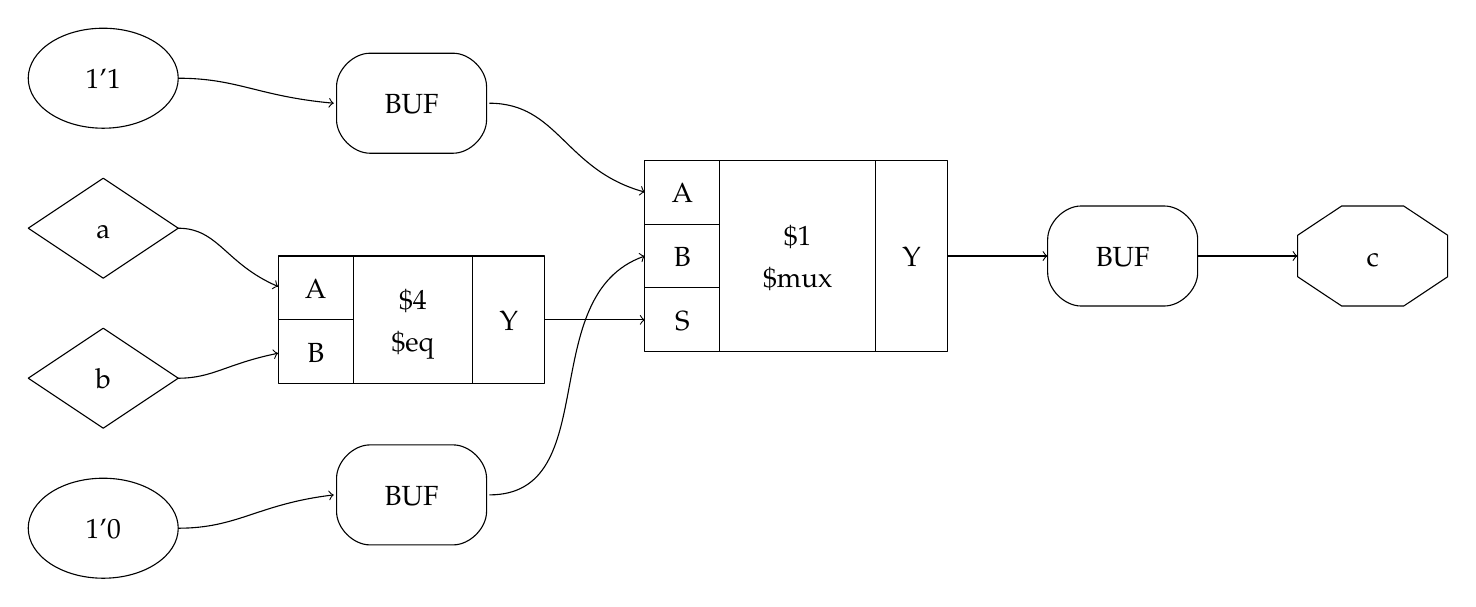
\begin{tikzpicture}[line join=bevel,anchor=base]%
\pgfsetcolor{black}
  % Edge: c11 -> c13
  \draw [->] (186.0bp,93.0bp) .. controls (198.0bp,93.0bp) and (203.25bp,93.0bp)  .. (222.0bp,93.0bp);
  % Edge: n6 -> c11
  \draw [->] (54.0bp,72.0bp) .. controls (66.498bp,72.0bp) and (71.257bp,77.169bp)  .. (90.0bp,81.0bp);
  % Edge: x2 -> n5
  \draw [->] (421.0bp,116.0bp) .. controls (433.0bp,116.0bp) and (438.25bp,116.0bp)  .. (457.0bp,116.0bp);
  % Edge: x1 -> c13
  \draw [->] (166.0bp,30.0bp) .. controls (207.69bp,30.0bp) and (181.85bp,101.85bp)  .. (222.0bp,116.0bp);
  % Edge: n7 -> c11
  \draw [->] (54.0bp,126.0bp) .. controls (68.471bp,126.0bp) and (70.998bp,113.18bp)  .. (90.0bp,105.0bp);
  % Edge: v0 -> x1
  \draw [->] (54.0bp,18.0bp) .. controls (75.676bp,18.0bp) and (82.586bp,26.702bp)  .. (110.0bp,30.0bp);
  % Edge: c13 -> x2
  \draw [->] (331.0bp,116.0bp) .. controls (343.0bp,116.0bp) and (348.25bp,116.0bp)  .. (367.0bp,116.0bp);
  % Edge: x4 -> c13
  \draw [->] (166.0bp,171.0bp) .. controls (190.86bp,171.0bp) and (193.16bp,146.94bp)  .. (222.0bp,139.0bp);
  % Edge: v3 -> x4
  \draw [->] (54.0bp,180.0bp) .. controls (75.466bp,180.0bp) and (82.702bp,173.47bp)  .. (110.0bp,171.0bp);
  % Node: v0
\begin{scope}
  \definecolor{strokecol}{rgb}{0.0,0.0,0.0};
  \pgfsetstrokecolor{strokecol}
  \draw (27.0bp,18.0bp) ellipse (27.0bp and 18.0bp);
  \draw (27.0bp,14.3bp) node {1'0};
\end{scope}
  % Node: x2
\begin{scope}
  \definecolor{strokecol}{rgb}{0.0,0.0,0.0};
  \pgfsetstrokecolor{strokecol}
  \draw (409.0bp,134.0bp) .. controls (409.0bp,134.0bp) and (379.0bp,134.0bp)  .. (379.0bp,134.0bp) .. controls (373.0bp,134.0bp) and (367.0bp,128.0bp)  .. (367.0bp,122.0bp) .. controls (367.0bp,122.0bp) and (367.0bp,110.0bp)  .. (367.0bp,110.0bp) .. controls (367.0bp,104.0bp) and (373.0bp,98.0bp)  .. (379.0bp,98.0bp) .. controls (379.0bp,98.0bp) and (409.0bp,98.0bp)  .. (409.0bp,98.0bp) .. controls (415.0bp,98.0bp) and (421.0bp,104.0bp)  .. (421.0bp,110.0bp) .. controls (421.0bp,110.0bp) and (421.0bp,122.0bp)  .. (421.0bp,122.0bp) .. controls (421.0bp,128.0bp) and (415.0bp,134.0bp)  .. (409.0bp,134.0bp);
  \draw (394.0bp,112.3bp) node {BUF};
\end{scope}
  % Node: v3
\begin{scope}
  \definecolor{strokecol}{rgb}{0.0,0.0,0.0};
  \pgfsetstrokecolor{strokecol}
  \draw (27.0bp,180.0bp) ellipse (27.0bp and 18.0bp);
  \draw (27.0bp,176.3bp) node {1'1};
\end{scope}
  % Node: x4
\begin{scope}
  \definecolor{strokecol}{rgb}{0.0,0.0,0.0};
  \pgfsetstrokecolor{strokecol}
  \draw (153.0bp,189.0bp) .. controls (153.0bp,189.0bp) and (123.0bp,189.0bp)  .. (123.0bp,189.0bp) .. controls (117.0bp,189.0bp) and (111.0bp,183.0bp)  .. (111.0bp,177.0bp) .. controls (111.0bp,177.0bp) and (111.0bp,165.0bp)  .. (111.0bp,165.0bp) .. controls (111.0bp,159.0bp) and (117.0bp,153.0bp)  .. (123.0bp,153.0bp) .. controls (123.0bp,153.0bp) and (153.0bp,153.0bp)  .. (153.0bp,153.0bp) .. controls (159.0bp,153.0bp) and (165.0bp,159.0bp)  .. (165.0bp,165.0bp) .. controls (165.0bp,165.0bp) and (165.0bp,177.0bp)  .. (165.0bp,177.0bp) .. controls (165.0bp,183.0bp) and (159.0bp,189.0bp)  .. (153.0bp,189.0bp);
  \draw (138.0bp,167.3bp) node {BUF};
\end{scope}
  % Node: c13
\begin{scope}
  \definecolor{strokecol}{rgb}{0.0,0.0,0.0};
  \pgfsetstrokecolor{strokecol}
  \draw (222.0bp,81.5bp) -- (222.0bp,150.5bp) -- (331.0bp,150.5bp) -- (331.0bp,81.5bp) -- cycle;
  \draw (222.0bp,127.5bp) -- (249.0bp,127.5bp);
  \draw (222.0bp,104.5bp) -- (249.0bp,104.5bp);
  \draw (249.0bp,81.5bp) -- (249.0bp,150.5bp);
  \draw (305.0bp,81.5bp) -- (305.0bp,150.5bp);
  \draw (235.5bp,135.3bp) node {A};
  \draw (235.5bp,112.3bp) node {B};
  \draw (235.5bp,89.3bp) node {S};
  \draw (277.0bp,119.8bp) node {\$1};
  \draw (277.0bp,104.8bp) node {\$mux};
  \draw (318.0bp,112.3bp) node {Y};
\end{scope}
  % Node: c11
\begin{scope}
  \definecolor{strokecol}{rgb}{0.0,0.0,0.0};
  \pgfsetstrokecolor{strokecol}
  \draw (90.0bp,70.0bp) -- (90.0bp,116.0bp) -- (186.0bp,116.0bp) -- (186.0bp,70.0bp) -- cycle;
  \draw (90.0bp,93.0bp) -- (117.0bp,93.0bp);
  \draw (117.0bp,70.0bp) -- (117.0bp,116.0bp);
  \draw (160.0bp,70.0bp) -- (160.0bp,116.0bp);
  \draw (103.5bp,100.8bp) node {A};
  \draw (103.5bp,77.8bp) node {B};
  \draw (138.5bp,96.8bp) node {\$4};
  \draw (138.5bp,81.8bp) node {\$eq};
  \draw (173.0bp,89.3bp) node {Y};
\end{scope}
  % Node: x1
\begin{scope}
  \definecolor{strokecol}{rgb}{0.0,0.0,0.0};
  \pgfsetstrokecolor{strokecol}
  \draw (153.0bp,48.0bp) .. controls (153.0bp,48.0bp) and (123.0bp,48.0bp)  .. (123.0bp,48.0bp) .. controls (117.0bp,48.0bp) and (111.0bp,42.0bp)  .. (111.0bp,36.0bp) .. controls (111.0bp,36.0bp) and (111.0bp,24.0bp)  .. (111.0bp,24.0bp) .. controls (111.0bp,18.0bp) and (117.0bp,12.0bp)  .. (123.0bp,12.0bp) .. controls (123.0bp,12.0bp) and (153.0bp,12.0bp)  .. (153.0bp,12.0bp) .. controls (159.0bp,12.0bp) and (165.0bp,18.0bp)  .. (165.0bp,24.0bp) .. controls (165.0bp,24.0bp) and (165.0bp,36.0bp)  .. (165.0bp,36.0bp) .. controls (165.0bp,42.0bp) and (159.0bp,48.0bp)  .. (153.0bp,48.0bp);
  \draw (138.0bp,26.3bp) node {BUF};
\end{scope}
  % Node: n5
\begin{scope}
  \definecolor{strokecol}{rgb}{0.0,0.0,0.0};
  \pgfsetstrokecolor{strokecol}
  \draw (511.0bp,108.54bp) -- (511.0bp,123.46bp) -- (495.18bp,134.0bp) -- (472.82bp,134.0bp) -- (457.0bp,123.46bp) -- (457.0bp,108.54bp) -- (472.82bp,98.0bp) -- (495.18bp,98.0bp) -- cycle;
  \draw (484.0bp,112.3bp) node {c};
\end{scope}
  % Node: n6
\begin{scope}
  \definecolor{strokecol}{rgb}{0.0,0.0,0.0};
  \pgfsetstrokecolor{strokecol}
  \draw (27.0bp,90.0bp) -- (0.0bp,72.0bp) -- (27.0bp,54.0bp) -- (54.0bp,72.0bp) -- cycle;
  \draw (27.0bp,68.3bp) node {b};
\end{scope}
  % Node: n7
\begin{scope}
  \definecolor{strokecol}{rgb}{0.0,0.0,0.0};
  \pgfsetstrokecolor{strokecol}
  \draw (27.0bp,144.0bp) -- (0.0bp,126.0bp) -- (27.0bp,108.0bp) -- (54.0bp,126.0bp) -- cycle;
  \draw (27.0bp,122.3bp) node {a};
\end{scope}
\end{tikzpicture}}%

    \label{fig:netlistIfCase}
\end{figure}

\subsection{Transformation algorithm -- Implementation details}

During traversal, every time the algorithm encounters an if or
case statement, it first examines the conditions and bodies of those
structures. Based on this information, the synthesizer pushes a netlist
object on top of a special stack which contains references to all
input and output ports as well as some additional information like,
for example, the corresponding control structure resulting in the
netlist.

\subsubsection{Introduced abstractions}
The netlist generator object carries around a stack containing
elements of type \CPP{stack_element_t}. As can be seen in file
\texttt{netlist_generator.h},
the stack is represented by a STL vector (cf. Glossary).
The algorithm only adds new elements using \CPP{push_back} and only
removes them with \CPP{pop_back}. However, the container must be a
vector, because the algorithm needs to be able to randomly access the
structure when synthesizing signal assignments.
%
\begin{lstlisting}[style=c++, caption={API of base stack element},
    label={lst:structElem}]
class NetlistGenerator {
public:
    // [...]
    struct stack_element_t {
        // constructors intentionally omitted
        std::map<string, netlist_element_t *> netlist;
        std::set<string> occurringSignals;
    };
    // [...]
};
\end{lstlisting}
%
Objects of type \CPP{struct_element_t} possess the API depicted in
listing \ref{lst:structElem}. There are three classes that inherit
from \CPP{struct_element_t}. As code \ref{lst:structElem} illustrates,
every element on the stack carries an association between signal IDs
(strings) and \CPP{netlist_element_t} objects as well as a list of all
driven Signals. These two members describe the core of the current
context.
For understandability purposes, code excerpt \ref{lst:structElemCase}
shows one of the derived classes used for the case statement
context. If the algorithm, for example, would encounter a case
statement like the one in \ref{lst:syncCaseStmt}, it'd first search
all possible traversal paths below the subjected case statement for
driven signals creating a set of those signals along the way. In the
context of \ref{lst:syncCaseStmt} this set would only contain one
element: \VH{A}. After that, the synthesizer would construct a
appropriate netlist for each of the set's elements. Finally, the set,
and the association of the signals with their muxer netlists is
packaged into an object of type \CPP{case_t} and pushed to the
stack (cf. file \texttt{netlist_generator.cc}, function
\CPP{executeIfStmt} in line 1041 and 1096, and function
\CPP{executeCaseStmt}).
%
\begin{lstlisting}[style=c++, caption={Case statement context class
      derived from stack_element_t}, label={lst:structElemCase}]
class NetlistGenerator {
public:
    // [...]
    struct case_t : stack_element_t {
        // constructors intentionally omitted
        Yosys::RTLIL::SigSpec curWhenAlternative;
    };
    // [...]
};
\end{lstlisting}
%
The synthesis algorithm does the same for if statements. Regarding
this, however, there are a few subtleties that need further attention.
As the synthesis results for \ref{lst:motSync}, \ref{lst:motLatch} and
\ref{lst:ifCase} show,
netlists
for if statements depend on two factors: The if condition and the set
of disjoint driven signals below the root of the respective if block.
Depending on the kind of condition of the if expression and the
distribution of the various statements inside the if block, the
contained signal assignments will be latched, clock accurately
synchronized or only carried through a simple
multiplexer. Consequently, there are two other classes implementing
the common interface presented in \ref{lst:structElem}: Class \CPP{if_dff_t}
and \CPP{if_latch_t}; both of which being declared by the \CPP{struct}
keyword making every member public by default as opposed to the
keyword \CPP{class}. The two classes, however, don't add anything new
to the base interface from \ref{lst:structElem} but only serve as a
kind of enumeration on the type level. This is a common design pattern
in functional programming and becomes feasible in C++ through the use
of the pattern matching library Mach7.
%TODO: Add reference to (1) design pattern func prog (2) mach7 chapter!

An open point of this elaboration still remains: Objects of type
\CPP{netlist_element_t}.
Like \CPP{stack_element_t}, a netlist element constructs an interface
using an abstract class. As \ref{lst:netlistElem} shows, this API
solely consists of one member named \CPP{output}. While some netlists
(e.g. Multiplexers or RAM blocks) can have inputs with attributes
associated with them, others only have one ore more \emph{anonymous}
inputs. For example, inputs of multiplexers have to carry the
selection semantics with them, because the synthesis algorithm needs
to know which muxer input corresponds to which choice in the
corresponding case statement. On the other hand, netlist parts, such
as latches or DFFs, only ever have one possible input.

\begin{lstlisting}[style=c++, caption={API of base netlist element},
    label={lst:netlistElem}]
class NetlistGenerator {
public:
    // [...]
    struct netlist_element_t {
        // constructors intentionally omitted
        Yosys::RTLIL::SigSpec output;
    };
    // [...]
};
\end{lstlisting}

\section{Current Limitations}
\label{sec:currentLimits}

The following is a non-comprehensive list of the most important
limitations of Yodl.

\begin{itemize}
    \item Only one \VH{architecture} definition per \VH{entity}
    declaration is allowed.
    \item \VH{Configurations} are not supported, because the
    underlying parser does not support this yet (cf. file
    \texttt{parse.y} in line 650).
    \item Yodl can't fully parse VHDL-2008. The code snippet below
    shows that, for example, a list of named arguments
    can't be used as a parameter list for a function called inside of
    an expression context (cf. \texttt{parse.y}).
    \begin{lstlisting}[style=vhdl]
architecture beh of ent is
   -- some decls
begin
   -- this should be parsable, but produces syntax error
   result <= foo(fnord => 3, foobar => 4)(3);

   -- this is parsable
    result <= foo(4, 3)(3);
end beh;
    \end{lstlisting}
    \item The synthesis algorithm is in a proof-of-concept pre-alpha
    state. It is untested and does not support signal or variable
    assignments with a vector subscription as left-hand side
    expression.
    \item The synthesis implementation can not translate variable
    assignments.
    \item The implementation is unable to cope with signal assignments
    like \VH{A <= A + 1}, i.e. assignments where the left-hand side
    also occurs, possibly multiple times, in the right-hand side
    expression.
    \item Synthesis of complex types (e.g. arrays of arrays of records
    \ldots) is not possible yet.
    \item The test suite is still rudimentary.
    \item The library and package concept was not considered in this work.
    \item The complex visibility rules from chapter 12 of
    \cite{IEEELRM} were not considered, since Yodl's base, vhdlpp,
    already came with an implementation of the scoping and visibility
    rules.
    \item Component instantiations can't be processed.
\end{itemize}

\chapter{Yodl -- Future work}
\section{Complete parser}
Section \ref{sec:currentLimits}
has already made clear, that the current parser solution is unfinished
and hence unable to parse the entirety of VHDL-2008. Thus, a very important
future goal of Yodl is to completely refactor or rewrite the parser
component. This is likely to be difficult because of the reasons
denoted in section \ref{sec:LexisAndSyntax}

The following section describes a tool that offers a lot of help if the
parser actually needs to be rewritten.

\subsection{BNFC and LBNF}
LBNF is a formalism which is based on the notation system BNF. The
L in LBNF stands for \emph{labeled}. Like BNF, the LBNF notation
is used to describe context free grammars, but unlike BNF it forces
the writer of the grammar to annotate every rule with a certain label.

For example, a simple expression grammar would be given in LBNF using
%
\begin{verbatim}
ENum . Exp3 ::= Integer ;
EMul . Exp2 ::= Exp2 "*" Exp3 ;
EPlu . Exp  ::= Exp "+" Exp2 ;
_    . Exp  ::= Exp2 ;
_    . Exp2 ::= Exp3 ;
_    . Exp3 ::= "(" Exp ")" ;
\end{verbatim}
%
BNFC is a program generator that takes LBNF code as input and produces
a complete frontend for the specified language, given the fact that
the grammar is sound. It can output language frontends in different
languages. At the time of this writing, BNFC is able to generate
Haskell, OCaml, C/C++, C-Sharp and Java code. For the previously
defined expression grammar, BNFC would output a flex and bison file
describing the scanner and parser part and a data model for the
abstract syntax tree. This data model in turn is used in the bison
file in order to actually create the said AST.
The according C++ classes for the grammar roughly look like listing
\ref{lst:bnfCpp}.
%
\begin{lstlisting}[style=c++, caption={Generated classes for
      expression grammar}, label={lst:bnfCpp}]
class Exp { public: virtual ~Exp() = default; };
class ENum : Exp { public: int value; ENum(int v) : value(v) {}  }
class EPlu : Exp {
    public: Exp *l, *r;
    EPlu(Exp *le, Exp *ri) : l(le), r(ri) { }
};
class EMul : Exp {
    public: Exp *l, *r;
    EMul(Exp *le, Exp *ri) : l(le), r(ri) { }
};
\end{lstlisting}
%
Normally the
above classes need to be handcrafted. This was done for Yodl'
parser. For anything but trivial
grammars, this task is tedious and error prone and should be
automated. Refer to \cite{LBNF} for details about the labeled BNF
formalism.

In the scope of this work, the entire VHDL-2008 BNF grammar has
already been
extracted from the official standard and completely \emph{translated}
into LBNF
(cf. \texttt{vhdlpp_parser/\-newparser/\-vhdl-2008/\-vhdl-2008-all.lbnf}).
%
%
%
%TODO: Proofread ab hier!!!
\section{Further grammar issues}
Yodl's current parser demonstrates how
especially reduce-reduce ambiguities can be dealt with. Simply put,
the parser needs to carry around a stack of scopes that it currently
processes (cf. \texttt{parse.y}, in particular line 366 pushes a new
scope frame and line 385 pops the same). Since every RR conflict
arises because of VHDL's use of
parentheses for array subscriptions, function/procedure calls and type
declarations (see listing \ref{lst:ambig}), the parser must know about
the scope it currently parses and every already declared/defined
symbol that scope possesses.
%
\begin{lstlisting}[style=vhdl, caption={Illustration of a common
      reduce-reduce conflict}, label={lst:ambig}]
function foo () is
begin
-- [...]
return "0000";
end function foo;

signal foo : std_logic_vector(7 downto 0);

foo(0); -- This could be parsed as
        -- 1. subscription of the vector foo
        -- 2. as call to the 0-ary function foo with one argument,
        --    which would be syntactically correct but semantical non-sense
        -- 3. as subscription of the return value resulting from the
        --    call to the 0-ary function foo with no argument
\end{lstlisting}
%
Hence, there is a solution for dealing with RR conflicts, but
what is about shift-reduce conflicts? They aren't allowed to lift the
grammar into the set of non-deterministically context free languages
because that would mean that even with Bison's GLR feature enabled %TODO:
                                %reference GLR
the grammar couldn't practically be processed. A parse-forest would
result from a parser run, which is completely inacceptable for
production-aspiring compilation systems.

For that reason, it must be proven that all SR conflicts together
(without the RR) indeed don't make the grammar non-determinstic.
This work does not provide any proof of that kind, because of the
complexity of the problem. The next paragraph, however, shows a first
approach.

GLR is a parser algorithm which, simply put, duplicates itself if it
encounters an ambiguity. Each parser then continues virtually in
parallel. Each duplicate can of course in turn duplicate and split
itself again and again if ambiguities are hit very often. \emph{If it is
guaranteed, that for each split only one of the duplicated parsers
succeeds, the parser produces only one parse tree for all inputs over
the grammar.} This condition is the core of the previously mentioned proof!
%TODO: Reference to Bison's GLR

\section{Complete VHDL support}

Currently Yodl is mainly an experimental project that does not support
VHDL specific language concepts such as packages, libraries,
components, configurations, generics and multiple architectures for a
given entity. As every industry-quality synthesis tool supports those
features, Yodl will support them too in the near future.

Packages and libraries are not trivial to implement because of the
complicated visibility rules described in chapter 12 of \cite{IEEELRM}
Especially generics provide for another challenge as 6.5.6.2 of
\cite{IEEELRM}
allows for generic functions and types which renders them more
like generics found in the programming language ADA as opposed to the
older concept where they were handled as simple constants.

\section{Far in the future}
The two last sections elaborate two projects that are probably very
work intensive. Hence, they won't be concerned until a first prototype
for full VHDL-2008 is released.

\subsection{Formal specification of VHDL's synthesis semantics}
The Book \cite{VHDLFORM}
already provides formal semantics for VHDL. Since its initial
release, which was in 1995, a lot of VHDL's synthesis semantics has
changed however. Because of that, a new specification becomes necessary.

\subsection{Regression based test suite}

As section \ref{sec:autoTests}
already states, the automation of tests is important to maintain a
correct code base. Compilers are among the most complex and complicated
software systems in existence which makes formal verification very
hard. Smoke tests, as they are implemented in the scope of this work,
are not quite sufficient because of their inadequate code
coverage. A Regression test suite in the sense of
\ref{sec:autoTestsReg} solves the coverage issue.

%\appendix
%%NO APPENDIX

%\chapter{First chapter of appendix}
%\label{a:somelabel}

%%% Local Variables: 
%%% mode: latex
%%% TeX-master: "thesis.tex"
%%% End: 


\cleardoublepage

\bibliographystyle{natger}
\bibliography{thesis}

\cleardoublepage


\footnotesize
\printindex


\end{document}
